% Options for packages loaded elsewhere
\PassOptionsToPackage{unicode}{hyperref}
\PassOptionsToPackage{hyphens}{url}
\PassOptionsToPackage{dvipsnames,svgnames,x11names}{xcolor}
%
\documentclass[
  letterpaper,
  DIV=11,
  numbers=noendperiod]{scrartcl}

\usepackage{amsmath,amssymb}
\usepackage{iftex}
\ifPDFTeX
  \usepackage[T1]{fontenc}
  \usepackage[utf8]{inputenc}
  \usepackage{textcomp} % provide euro and other symbols
\else % if luatex or xetex
  \usepackage{unicode-math}
  \defaultfontfeatures{Scale=MatchLowercase}
  \defaultfontfeatures[\rmfamily]{Ligatures=TeX,Scale=1}
\fi
\usepackage{lmodern}
\ifPDFTeX\else  
    % xetex/luatex font selection
\fi
% Use upquote if available, for straight quotes in verbatim environments
\IfFileExists{upquote.sty}{\usepackage{upquote}}{}
\IfFileExists{microtype.sty}{% use microtype if available
  \usepackage[]{microtype}
  \UseMicrotypeSet[protrusion]{basicmath} % disable protrusion for tt fonts
}{}
\makeatletter
\@ifundefined{KOMAClassName}{% if non-KOMA class
  \IfFileExists{parskip.sty}{%
    \usepackage{parskip}
  }{% else
    \setlength{\parindent}{0pt}
    \setlength{\parskip}{6pt plus 2pt minus 1pt}}
}{% if KOMA class
  \KOMAoptions{parskip=half}}
\makeatother
\usepackage{xcolor}
\ifLuaTeX
  \usepackage{luacolor}
  \usepackage[soul]{lua-ul}
\else
  \usepackage{soul}
  
\fi
\setlength{\emergencystretch}{3em} % prevent overfull lines
\setcounter{secnumdepth}{-\maxdimen} % remove section numbering
% Make \paragraph and \subparagraph free-standing
\ifx\paragraph\undefined\else
  \let\oldparagraph\paragraph
  \renewcommand{\paragraph}[1]{\oldparagraph{#1}\mbox{}}
\fi
\ifx\subparagraph\undefined\else
  \let\oldsubparagraph\subparagraph
  \renewcommand{\subparagraph}[1]{\oldsubparagraph{#1}\mbox{}}
\fi

\usepackage{color}
\usepackage{fancyvrb}
\newcommand{\VerbBar}{|}
\newcommand{\VERB}{\Verb[commandchars=\\\{\}]}
\DefineVerbatimEnvironment{Highlighting}{Verbatim}{commandchars=\\\{\}}
% Add ',fontsize=\small' for more characters per line
\usepackage{framed}
\definecolor{shadecolor}{RGB}{241,243,245}
\newenvironment{Shaded}{\begin{snugshade}}{\end{snugshade}}
\newcommand{\AlertTok}[1]{\textcolor[rgb]{0.68,0.00,0.00}{#1}}
\newcommand{\AnnotationTok}[1]{\textcolor[rgb]{0.37,0.37,0.37}{#1}}
\newcommand{\AttributeTok}[1]{\textcolor[rgb]{0.40,0.45,0.13}{#1}}
\newcommand{\BaseNTok}[1]{\textcolor[rgb]{0.68,0.00,0.00}{#1}}
\newcommand{\BuiltInTok}[1]{\textcolor[rgb]{0.00,0.23,0.31}{#1}}
\newcommand{\CharTok}[1]{\textcolor[rgb]{0.13,0.47,0.30}{#1}}
\newcommand{\CommentTok}[1]{\textcolor[rgb]{0.37,0.37,0.37}{#1}}
\newcommand{\CommentVarTok}[1]{\textcolor[rgb]{0.37,0.37,0.37}{\textit{#1}}}
\newcommand{\ConstantTok}[1]{\textcolor[rgb]{0.56,0.35,0.01}{#1}}
\newcommand{\ControlFlowTok}[1]{\textcolor[rgb]{0.00,0.23,0.31}{#1}}
\newcommand{\DataTypeTok}[1]{\textcolor[rgb]{0.68,0.00,0.00}{#1}}
\newcommand{\DecValTok}[1]{\textcolor[rgb]{0.68,0.00,0.00}{#1}}
\newcommand{\DocumentationTok}[1]{\textcolor[rgb]{0.37,0.37,0.37}{\textit{#1}}}
\newcommand{\ErrorTok}[1]{\textcolor[rgb]{0.68,0.00,0.00}{#1}}
\newcommand{\ExtensionTok}[1]{\textcolor[rgb]{0.00,0.23,0.31}{#1}}
\newcommand{\FloatTok}[1]{\textcolor[rgb]{0.68,0.00,0.00}{#1}}
\newcommand{\FunctionTok}[1]{\textcolor[rgb]{0.28,0.35,0.67}{#1}}
\newcommand{\ImportTok}[1]{\textcolor[rgb]{0.00,0.46,0.62}{#1}}
\newcommand{\InformationTok}[1]{\textcolor[rgb]{0.37,0.37,0.37}{#1}}
\newcommand{\KeywordTok}[1]{\textcolor[rgb]{0.00,0.23,0.31}{#1}}
\newcommand{\NormalTok}[1]{\textcolor[rgb]{0.00,0.23,0.31}{#1}}
\newcommand{\OperatorTok}[1]{\textcolor[rgb]{0.37,0.37,0.37}{#1}}
\newcommand{\OtherTok}[1]{\textcolor[rgb]{0.00,0.23,0.31}{#1}}
\newcommand{\PreprocessorTok}[1]{\textcolor[rgb]{0.68,0.00,0.00}{#1}}
\newcommand{\RegionMarkerTok}[1]{\textcolor[rgb]{0.00,0.23,0.31}{#1}}
\newcommand{\SpecialCharTok}[1]{\textcolor[rgb]{0.37,0.37,0.37}{#1}}
\newcommand{\SpecialStringTok}[1]{\textcolor[rgb]{0.13,0.47,0.30}{#1}}
\newcommand{\StringTok}[1]{\textcolor[rgb]{0.13,0.47,0.30}{#1}}
\newcommand{\VariableTok}[1]{\textcolor[rgb]{0.07,0.07,0.07}{#1}}
\newcommand{\VerbatimStringTok}[1]{\textcolor[rgb]{0.13,0.47,0.30}{#1}}
\newcommand{\WarningTok}[1]{\textcolor[rgb]{0.37,0.37,0.37}{\textit{#1}}}

\providecommand{\tightlist}{%
  \setlength{\itemsep}{0pt}\setlength{\parskip}{0pt}}\usepackage{longtable,booktabs,array}
\usepackage{calc} % for calculating minipage widths
% Correct order of tables after \paragraph or \subparagraph
\usepackage{etoolbox}
\makeatletter
\patchcmd\longtable{\par}{\if@noskipsec\mbox{}\fi\par}{}{}
\makeatother
% Allow footnotes in longtable head/foot
\IfFileExists{footnotehyper.sty}{\usepackage{footnotehyper}}{\usepackage{footnote}}
\makesavenoteenv{longtable}
\usepackage{graphicx}
\makeatletter
\def\maxwidth{\ifdim\Gin@nat@width>\linewidth\linewidth\else\Gin@nat@width\fi}
\def\maxheight{\ifdim\Gin@nat@height>\textheight\textheight\else\Gin@nat@height\fi}
\makeatother
% Scale images if necessary, so that they will not overflow the page
% margins by default, and it is still possible to overwrite the defaults
% using explicit options in \includegraphics[width, height, ...]{}
\setkeys{Gin}{width=\maxwidth,height=\maxheight,keepaspectratio}
% Set default figure placement to htbp
\makeatletter
\def\fps@figure{htbp}
\makeatother

\KOMAoption{captions}{tableheading}
\makeatletter
\@ifpackageloaded{tcolorbox}{}{\usepackage[skins,breakable]{tcolorbox}}
\@ifpackageloaded{fontawesome5}{}{\usepackage{fontawesome5}}
\definecolor{quarto-callout-color}{HTML}{909090}
\definecolor{quarto-callout-note-color}{HTML}{0758E5}
\definecolor{quarto-callout-important-color}{HTML}{CC1914}
\definecolor{quarto-callout-warning-color}{HTML}{EB9113}
\definecolor{quarto-callout-tip-color}{HTML}{00A047}
\definecolor{quarto-callout-caution-color}{HTML}{FC5300}
\definecolor{quarto-callout-color-frame}{HTML}{acacac}
\definecolor{quarto-callout-note-color-frame}{HTML}{4582ec}
\definecolor{quarto-callout-important-color-frame}{HTML}{d9534f}
\definecolor{quarto-callout-warning-color-frame}{HTML}{f0ad4e}
\definecolor{quarto-callout-tip-color-frame}{HTML}{02b875}
\definecolor{quarto-callout-caution-color-frame}{HTML}{fd7e14}
\makeatother
\makeatletter
\@ifpackageloaded{caption}{}{\usepackage{caption}}
\AtBeginDocument{%
\ifdefined\contentsname
  \renewcommand*\contentsname{Table of contents}
\else
  \newcommand\contentsname{Table of contents}
\fi
\ifdefined\listfigurename
  \renewcommand*\listfigurename{List of Figures}
\else
  \newcommand\listfigurename{List of Figures}
\fi
\ifdefined\listtablename
  \renewcommand*\listtablename{List of Tables}
\else
  \newcommand\listtablename{List of Tables}
\fi
\ifdefined\figurename
  \renewcommand*\figurename{Figure}
\else
  \newcommand\figurename{Figure}
\fi
\ifdefined\tablename
  \renewcommand*\tablename{Table}
\else
  \newcommand\tablename{Table}
\fi
}
\@ifpackageloaded{float}{}{\usepackage{float}}
\floatstyle{ruled}
\@ifundefined{c@chapter}{\newfloat{codelisting}{h}{lop}}{\newfloat{codelisting}{h}{lop}[chapter]}
\floatname{codelisting}{Listing}
\newcommand*\listoflistings{\listof{codelisting}{List of Listings}}
\makeatother
\makeatletter
\makeatother
\makeatletter
\@ifpackageloaded{caption}{}{\usepackage{caption}}
\@ifpackageloaded{subcaption}{}{\usepackage{subcaption}}
\makeatother
\ifLuaTeX
  \usepackage{selnolig}  % disable illegal ligatures
\fi
\usepackage{bookmark}

\IfFileExists{xurl.sty}{\usepackage{xurl}}{} % add URL line breaks if available
\urlstyle{same} % disable monospaced font for URLs
\hypersetup{
  pdftitle={Climate resilience requires equitable access to quality green energy jobs. The City of Saint Paul is at the forefront.},
  pdfauthor={Elham Ali},
  pdfkeywords={climate justice, climate-ready workforce, green
jobs, climate change, equity},
  colorlinks=true,
  linkcolor={blue},
  filecolor={Maroon},
  citecolor={Blue},
  urlcolor={Blue},
  pdfcreator={LaTeX via pandoc}}

\title{Climate resilience requires equitable access to quality green
energy jobs. The City of Saint Paul is at the forefront.}
\author{Elham Ali}
\date{2024-09-19}

\begin{document}
\maketitle
\begin{abstract}
Minnesota, particularly the City of Saint Paul, has seen a surge in
climate resilience funding aimed at expanding green energy job
opportunities. However, BIPOC communities remain underrepresented in
these jobs and disproportionately suffer from the adverse effects of
human-driven climate change.
\end{abstract}

\subsection{Background}\label{background}

This analysis looks at access to green energy jobs (like energy
efficiency, renewable energy, and green construction) by race/ethnicity,
gender, education, and income in St.~Paul, Minnesota, USA.

\subsection{Questions}\label{questions}

Here are some of the questions I will explore using different datasets:

\begin{itemize}
\tightlist
\item
  How much climate resilience funding has St.~Paul received?
\item
  What specific green jobs are being created in St.~Paul (e.g., energy
  efficiency, renewable energy, green construction)?
\item
  What is the quality of these jobs? How much do they pay? What
  qualifications are needed (education and experience)?
\item
  Who is getting these jobs, based on education, race/ethnicity, gender,
  and income levels?
\end{itemize}

\subsection{Data Sources}\label{data-sources}

The data for this project comes from:

\begin{itemize}
\tightlist
\item
  The National Center for O*NET Development
\item
  2023 Occupational Employment and Wage Survey
\item
  Urban Institute 11 elements of job quality: Clean Energy Job Quality
  and Education Data
\item
  National and local demographic data from the 2022 American Community
  Survey Public Use Microdata Sample (ACS PUMS)
\item
  US Census Bureau's 2023 QuickFacts tool
\item
  Invest.gov
\item
  Geocorr from the Missouri Census Data Center
\end{itemize}

I will reduce each large dataset to focus only on questions related to
green jobs and job quality. Please note that some datasets have already
been pre-processed in Python with specific filters applied. You can find
the original raw datasets in the data folder for reference.

\subsection{Analysis}\label{analysis}

I will look at each question one by one and clean the data as I go. Some
datasets might need to be combined, so I will organize the data during
the analysis before exploring the results.

\subsubsection{Load packages and
libraries}\label{load-packages-and-libraries}

\begin{Shaded}
\begin{Highlighting}[]
\DocumentationTok{\#\# For folder structure}
\FunctionTok{library}\NormalTok{(here)}
\end{Highlighting}
\end{Shaded}

\begin{verbatim}
here() starts at /Users/elhamali/Documents/Data Projects/climate-equity-workforce
\end{verbatim}

\begin{Shaded}
\begin{Highlighting}[]
\FunctionTok{library}\NormalTok{(ezknitr)}

\DocumentationTok{\#\# For data import/cleaning}
\FunctionTok{library}\NormalTok{(tidyverse)}
\end{Highlighting}
\end{Shaded}

\begin{verbatim}
-- Attaching core tidyverse packages ------------------------ tidyverse 2.0.0 --
v dplyr     1.1.4     v readr     2.1.5
v forcats   1.0.0     v stringr   1.5.1
v ggplot2   3.5.1     v tibble    3.2.1
v lubridate 1.9.3     v tidyr     1.3.1
v purrr     1.0.2     
\end{verbatim}

\begin{verbatim}
-- Conflicts ------------------------------------------ tidyverse_conflicts() --
x dplyr::filter() masks stats::filter()
x dplyr::lag()    masks stats::lag()
i Use the conflicted package (<http://conflicted.r-lib.org/>) to force all conflicts to become errors
\end{verbatim}

\begin{Shaded}
\begin{Highlighting}[]
\FunctionTok{library}\NormalTok{(purrr)}
\FunctionTok{library}\NormalTok{(rlang)}
\end{Highlighting}
\end{Shaded}

\begin{verbatim}

Attaching package: 'rlang'

The following objects are masked from 'package:purrr':

    %@%, flatten, flatten_chr, flatten_dbl, flatten_int, flatten_lgl,
    flatten_raw, invoke, splice
\end{verbatim}

\begin{Shaded}
\begin{Highlighting}[]
\FunctionTok{library}\NormalTok{(forcats)}
\FunctionTok{library}\NormalTok{(readxl)}

\DocumentationTok{\#\# For graphing}
\FunctionTok{library}\NormalTok{(highcharter)}
\end{Highlighting}
\end{Shaded}

\begin{verbatim}
Registered S3 method overwritten by 'quantmod':
  method            from
  as.zoo.data.frame zoo 
\end{verbatim}

\begin{Shaded}
\begin{Highlighting}[]
\FunctionTok{library}\NormalTok{(igraph)}
\end{Highlighting}
\end{Shaded}

\begin{verbatim}

Attaching package: 'igraph'

The following object is masked from 'package:rlang':

    is_named

The following objects are masked from 'package:lubridate':

    %--%, union

The following objects are masked from 'package:dplyr':

    as_data_frame, groups, union

The following objects are masked from 'package:purrr':

    compose, simplify

The following object is masked from 'package:tidyr':

    crossing

The following object is masked from 'package:tibble':

    as_data_frame

The following objects are masked from 'package:stats':

    decompose, spectrum

The following object is masked from 'package:base':

    union
\end{verbatim}

\begin{Shaded}
\begin{Highlighting}[]
\FunctionTok{library}\NormalTok{(RColorBrewer)}
\FunctionTok{library}\NormalTok{(htmlwidgets)}
\FunctionTok{library}\NormalTok{(gt)}
\CommentTok{\# library(viridis)}
\end{Highlighting}
\end{Shaded}

\textsubscript{Source:
\href{https://beeckcenter.github.io/climate-equity-workforce/index-preview.html}{Article
Notebook}}

\subsubsection{1. Climate Resilience Funding for
St.~Paul}\label{climate-resilience-funding-for-st.-paul}

\begin{tcolorbox}[enhanced jigsaw, coltitle=black, opacitybacktitle=0.6, rightrule=.15mm, colframe=quarto-callout-note-color-frame, bottomtitle=1mm, title=\textcolor{quarto-callout-note-color}{\faInfo}\hspace{0.5em}{RQ 1: How much climate resilience funding has the City of Saint Paul
received?}, breakable, colback=white, toptitle=1mm, titlerule=0mm, arc=.35mm, opacityback=0, left=2mm, bottomrule=.15mm, toprule=.15mm, colbacktitle=quarto-callout-note-color!10!white, leftrule=.75mm]

As of June 2024, \textbf{Minnesota} received a total of \$7,101,423,527
in funding for climate resilience, while \textbf{St.~Paul} received
\$446,286,762. Specifically, as of January 2024, St.~Paul has secured
\$433,028,012 from the Bipartisan Infrastructure Law (BIL) and
\$13,258,750 from the Inflation Reduction Act (IRA) for \textbf{climate
resilience efforts.}

St.~Paul's funding makes up \textbf{6.28\%} of Minnesota's total climate
resilience funding. Nearly \textbf{95\% of St.~Paul's funding i}s
allocated to \textbf{transportation} \textbf{projects}, with clean
energy, buildings, and manufacturing receiving \textbf{less than 2\% of
the total}. It's like filling up a swimming pool with water but using
only a small 8 oz glass for clean energy, buildings, and manufacturing.

As of January 2024, St.~Paul received \textbf{\$8,337,843 from the BIL}
and \textbf{\$200,000 from the IRA} specifically for investments in
clean energy, buildings, and manufacturing.

\end{tcolorbox}

\begin{Shaded}
\begin{Highlighting}[]
\CommentTok{\# Import data}
\NormalTok{funding }\OtherTok{\textless{}{-}} \FunctionTok{read\_csv}\NormalTok{(}\FunctionTok{here}\NormalTok{(}\StringTok{"processed\_data"}\NormalTok{, }\StringTok{"FundingSummary.csv"}\NormalTok{))}
\end{Highlighting}
\end{Shaded}

\begin{verbatim}
Warning: One or more parsing issues, call `problems()` on your data frame for details,
e.g.:
  dat <- vroom(...)
  problems(dat)
\end{verbatim}

\begin{verbatim}
Rows: 49535 Columns: 15
-- Column specification --------------------------------------------------------
Delimiter: ","
chr (14): Agency Name, Bureau Name, Program Name, Category, Subcategory, Pro...
dbl  (1): Unique ID

i Use `spec()` to retrieve the full column specification for this data.
i Specify the column types or set `show_col_types = FALSE` to quiet this message.
\end{verbatim}

\begin{Shaded}
\begin{Highlighting}[]
\FunctionTok{saveRDS}\NormalTok{(funding, }\FunctionTok{here}\NormalTok{(}\StringTok{"processed\_data"}\NormalTok{, }\StringTok{"funding.rds"}\NormalTok{))}

\NormalTok{funding }\OtherTok{\textless{}{-}} \FunctionTok{readRDS}\NormalTok{(}\FunctionTok{here}\NormalTok{(}\StringTok{"processed\_data"}\NormalTok{, }\StringTok{"funding.rds"}\NormalTok{))}
\end{Highlighting}
\end{Shaded}

\textsubscript{Source:
\href{https://beeckcenter.github.io/climate-equity-workforce/index-preview.html}{Article
Notebook}}

\begin{Shaded}
\begin{Highlighting}[]
\DocumentationTok{\#\#\# Convert the \textasciigrave{}Funding Amount\textasciigrave{} to numeric and handling commas in the values}

\NormalTok{funding }\OtherTok{\textless{}{-}}\NormalTok{ funding }\SpecialCharTok{\%\textgreater{}\%}
  \FunctionTok{mutate}\NormalTok{(}\StringTok{\textasciigrave{}}\AttributeTok{Funding Amount}\StringTok{\textasciigrave{}} \OtherTok{=} \FunctionTok{as.numeric}\NormalTok{(}\FunctionTok{gsub}\NormalTok{(}\StringTok{","}\NormalTok{, }\StringTok{""}\NormalTok{, }\StringTok{\textasciigrave{}}\AttributeTok{Funding Amount}\StringTok{\textasciigrave{}}\NormalTok{)))}
\end{Highlighting}
\end{Shaded}

\begin{verbatim}
Warning: There was 1 warning in `mutate()`.
i In argument: `Funding Amount = as.numeric(gsub(",", "", `Funding Amount`))`.
Caused by warning:
! NAs introduced by coercion
\end{verbatim}

\textsubscript{Source:
\href{https://beeckcenter.github.io/climate-equity-workforce/index-preview.html}{Article
Notebook}}

\paragraph{Filter for MN State and City of
St.~Paul}\label{filter-for-mn-state-and-city-of-st.-paul}

First, I will filter the dataset by State: \textbf{Minnesota}, and then
narrow it down further to focus on the \textbf{City of St.~Paul} and the
surrounding region. Please note that St.~Paul is part of the
\textbf{Minneapolis-St.~Paul-Bloomington, MN-WI} region, so I'll ensure
it's included within that larger metropolitan area.

\begin{Shaded}
\begin{Highlighting}[]
\CommentTok{\# Filter for Minnesota funding}
\NormalTok{minnesota\_funding }\OtherTok{\textless{}{-}}\NormalTok{ funding }\SpecialCharTok{\%\textgreater{}\%}
  \FunctionTok{filter}\NormalTok{(State }\SpecialCharTok{==} \StringTok{"Minnesota"}\NormalTok{)}

\FunctionTok{saveRDS}\NormalTok{(minnesota\_funding, }\FunctionTok{here}\NormalTok{(}\StringTok{"processed\_data"}\NormalTok{, }\StringTok{"minnesota\_funding.rds"}\NormalTok{))}
\end{Highlighting}
\end{Shaded}

\textsubscript{Source:
\href{https://beeckcenter.github.io/climate-equity-workforce/index-preview.html}{Article
Notebook}}

\begin{Shaded}
\begin{Highlighting}[]
\CommentTok{\# Further filter for St. Paul, considering variations in city names}
\NormalTok{st\_paul\_funding }\OtherTok{\textless{}{-}}\NormalTok{ minnesota\_funding }\SpecialCharTok{\%\textgreater{}\%}
  \FunctionTok{filter}\NormalTok{(}\FunctionTok{str\_detect}\NormalTok{(City, }\FunctionTok{regex}\NormalTok{(}\StringTok{"Saint Paul|St. Paul|South St. Paul|Minneapolis{-}{-}St. Paul|Minneapolis{-}St. Paul"}\NormalTok{, }\AttributeTok{ignore\_case =} \ConstantTok{TRUE}\NormalTok{)))}

\FunctionTok{saveRDS}\NormalTok{(st\_paul\_funding, }\FunctionTok{here}\NormalTok{(}\StringTok{"processed\_data"}\NormalTok{, }\StringTok{"st\_paul\_funding.rds"}\NormalTok{))}

\CommentTok{\# glimpse(st\_paul\_funding)}
\end{Highlighting}
\end{Shaded}

\textsubscript{Source:
\href{https://beeckcenter.github.io/climate-equity-workforce/index-preview.html}{Article
Notebook}}

\paragraph{Calculate funding for MN State and City of
St.~Paul}\label{calculate-funding-for-mn-state-and-city-of-st.-paul}

\begin{Shaded}
\begin{Highlighting}[]
\CommentTok{\# Set options to avoid scientific notation}
\FunctionTok{options}\NormalTok{(}\AttributeTok{scipen =} \DecValTok{999}\NormalTok{)}

\CommentTok{\# Load Minnesota and St. Paul data}
\NormalTok{minnesota\_funding }\OtherTok{\textless{}{-}} \FunctionTok{readRDS}\NormalTok{(}\FunctionTok{here}\NormalTok{(}\StringTok{"processed\_data"}\NormalTok{, }\StringTok{"minnesota\_funding.rds"}\NormalTok{))}
\NormalTok{st\_paul\_funding }\OtherTok{\textless{}{-}} \FunctionTok{readRDS}\NormalTok{(}\FunctionTok{here}\NormalTok{(}\StringTok{"processed\_data"}\NormalTok{, }\StringTok{"st\_paul\_funding.rds"}\NormalTok{))}

\CommentTok{\# Calculate total funding for Minnesota}
\NormalTok{total\_minnesota\_funding }\OtherTok{\textless{}{-}}\NormalTok{ minnesota\_funding }\SpecialCharTok{\%\textgreater{}\%}
  \FunctionTok{summarise}\NormalTok{(}\AttributeTok{total\_funding =} \FunctionTok{sum}\NormalTok{(}\StringTok{\textasciigrave{}}\AttributeTok{Funding Amount}\StringTok{\textasciigrave{}}\NormalTok{, }\AttributeTok{na.rm =} \ConstantTok{TRUE}\NormalTok{))}

\FunctionTok{cat}\NormalTok{(}\StringTok{"The total amount of funding Minnesota received for climate as of June 2024 is $"}\NormalTok{, }
    \FunctionTok{format}\NormalTok{(total\_minnesota\_funding}\SpecialCharTok{$}\NormalTok{total\_funding, }\AttributeTok{big.mark =} \StringTok{","}\NormalTok{), }\StringTok{"}\SpecialCharTok{\textbackslash{}n}\StringTok{"}\NormalTok{)}
\end{Highlighting}
\end{Shaded}

\begin{verbatim}
The total amount of funding Minnesota received for climate as of June 2024 is $ 7,101,423,527 
\end{verbatim}

\begin{Shaded}
\begin{Highlighting}[]
\CommentTok{\# Calculate total funding for St. Paul}
\NormalTok{total\_st\_paul\_funding }\OtherTok{\textless{}{-}}\NormalTok{ st\_paul\_funding }\SpecialCharTok{\%\textgreater{}\%}
  \FunctionTok{summarise}\NormalTok{(}\AttributeTok{total\_funding =} \FunctionTok{sum}\NormalTok{(}\StringTok{\textasciigrave{}}\AttributeTok{Funding Amount}\StringTok{\textasciigrave{}}\NormalTok{, }\AttributeTok{na.rm =} \ConstantTok{TRUE}\NormalTok{))}

\FunctionTok{cat}\NormalTok{(}\StringTok{"The total amount of funding St. Paul received for climate as of June 2024 is $"}\NormalTok{, }
    \FunctionTok{format}\NormalTok{(total\_st\_paul\_funding}\SpecialCharTok{$}\NormalTok{total\_funding, }\AttributeTok{big.mark =} \StringTok{","}\NormalTok{), }\StringTok{"}\SpecialCharTok{\textbackslash{}n}\StringTok{"}\NormalTok{)}
\end{Highlighting}
\end{Shaded}

\begin{verbatim}
The total amount of funding St. Paul received for climate as of June 2024 is $ 446,286,762 
\end{verbatim}

\begin{Shaded}
\begin{Highlighting}[]
\CommentTok{\# Calculate total funds by funding source for St. Paul}
\NormalTok{source\_st\_paul\_funding }\OtherTok{\textless{}{-}}\NormalTok{ st\_paul\_funding }\SpecialCharTok{\%\textgreater{}\%}
  \FunctionTok{group\_by}\NormalTok{(}\StringTok{\textasciigrave{}}\AttributeTok{Funding Source}\StringTok{\textasciigrave{}}\NormalTok{) }\SpecialCharTok{\%\textgreater{}\%}
  \FunctionTok{summarise}\NormalTok{(}\AttributeTok{total\_funding =} \FunctionTok{sum}\NormalTok{(}\StringTok{\textasciigrave{}}\AttributeTok{Funding Amount}\StringTok{\textasciigrave{}}\NormalTok{, }\AttributeTok{na.rm =} \ConstantTok{TRUE}\NormalTok{))}

\CommentTok{\# Calculate specific totals for BIL and IRA}
\NormalTok{bil\_funding }\OtherTok{\textless{}{-}}\NormalTok{ st\_paul\_funding }\SpecialCharTok{\%\textgreater{}\%}
  \FunctionTok{filter}\NormalTok{(}\StringTok{\textasciigrave{}}\AttributeTok{Funding Source}\StringTok{\textasciigrave{}} \SpecialCharTok{==} \StringTok{"BIL"}\NormalTok{) }\SpecialCharTok{\%\textgreater{}\%}
  \FunctionTok{summarise}\NormalTok{(}\AttributeTok{total\_bil =} \FunctionTok{sum}\NormalTok{(}\StringTok{\textasciigrave{}}\AttributeTok{Funding Amount}\StringTok{\textasciigrave{}}\NormalTok{, }\AttributeTok{na.rm =} \ConstantTok{TRUE}\NormalTok{))}

\NormalTok{ira\_funding }\OtherTok{\textless{}{-}}\NormalTok{ st\_paul\_funding }\SpecialCharTok{\%\textgreater{}\%}
  \FunctionTok{filter}\NormalTok{(}\StringTok{\textasciigrave{}}\AttributeTok{Funding Source}\StringTok{\textasciigrave{}} \SpecialCharTok{==} \StringTok{"IRA"}\NormalTok{) }\SpecialCharTok{\%\textgreater{}\%}
  \FunctionTok{summarise}\NormalTok{(}\AttributeTok{total\_ira =} \FunctionTok{sum}\NormalTok{(}\StringTok{\textasciigrave{}}\AttributeTok{Funding Amount}\StringTok{\textasciigrave{}}\NormalTok{, }\AttributeTok{na.rm =} \ConstantTok{TRUE}\NormalTok{))}

\CommentTok{\# Print specific funding from BIL and IRA}
\FunctionTok{cat}\NormalTok{(}\StringTok{"As of January 2024, St. Paul has been allocated $"}\NormalTok{, }
    \FunctionTok{format}\NormalTok{(bil\_funding}\SpecialCharTok{$}\NormalTok{total\_bil, }\AttributeTok{big.mark =} \StringTok{","}\NormalTok{, }\AttributeTok{scientific =} \ConstantTok{FALSE}\NormalTok{), }
    \StringTok{" from the Bipartisan Infrastructure Law (BIL) and $"}\NormalTok{, }
    \FunctionTok{format}\NormalTok{(ira\_funding}\SpecialCharTok{$}\NormalTok{total\_ira, }\AttributeTok{big.mark =} \StringTok{","}\NormalTok{, }\AttributeTok{scientific =} \ConstantTok{FALSE}\NormalTok{), }
    \StringTok{" from the Inflation Reduction Act (IRA).}\SpecialCharTok{\textbackslash{}n}\StringTok{"}\NormalTok{)}
\end{Highlighting}
\end{Shaded}

\begin{verbatim}
As of January 2024, St. Paul has been allocated $ 433,028,012  from the Bipartisan Infrastructure Law (BIL) and $ 13,258,750  from the Inflation Reduction Act (IRA).
\end{verbatim}

\begin{Shaded}
\begin{Highlighting}[]
\CommentTok{\# Filter for the specific category \textquotesingle{}Clean Energy, Buildings, and Manufacturing\textquotesingle{}}
\NormalTok{st\_paul\_clean\_energy\_funding }\OtherTok{\textless{}{-}}\NormalTok{ st\_paul\_funding }\SpecialCharTok{\%\textgreater{}\%}
  \FunctionTok{filter}\NormalTok{(Category }\SpecialCharTok{==} \StringTok{"Clean Energy, Buildings, and Manufacturing"}\NormalTok{)}

\CommentTok{\# Calculate total funds by funding source for the specific category}
\NormalTok{source\_st\_paul\_clean\_energy\_funding }\OtherTok{\textless{}{-}}\NormalTok{ st\_paul\_clean\_energy\_funding }\SpecialCharTok{\%\textgreater{}\%}
  \FunctionTok{group\_by}\NormalTok{(}\StringTok{\textasciigrave{}}\AttributeTok{Funding Source}\StringTok{\textasciigrave{}}\NormalTok{) }\SpecialCharTok{\%\textgreater{}\%}
  \FunctionTok{summarise}\NormalTok{(}\AttributeTok{total\_funding =} \FunctionTok{sum}\NormalTok{(}\StringTok{\textasciigrave{}}\AttributeTok{Funding Amount}\StringTok{\textasciigrave{}}\NormalTok{, }\AttributeTok{na.rm =} \ConstantTok{TRUE}\NormalTok{))}

\CommentTok{\# Calculate total funding across all sources for the specific category}
\NormalTok{total\_st\_paul\_clean\_energy\_funding }\OtherTok{\textless{}{-}}\NormalTok{ st\_paul\_clean\_energy\_funding }\SpecialCharTok{\%\textgreater{}\%}
  \FunctionTok{summarise}\NormalTok{(}\AttributeTok{total\_funding =} \FunctionTok{sum}\NormalTok{(}\StringTok{\textasciigrave{}}\AttributeTok{Funding Amount}\StringTok{\textasciigrave{}}\NormalTok{, }\AttributeTok{na.rm =} \ConstantTok{TRUE}\NormalTok{))}

\CommentTok{\# Calculate specific totals for BIL and IRA in the specific category}
\NormalTok{bil\_clean\_energy\_funding }\OtherTok{\textless{}{-}}\NormalTok{ st\_paul\_clean\_energy\_funding }\SpecialCharTok{\%\textgreater{}\%}
  \FunctionTok{filter}\NormalTok{(}\StringTok{\textasciigrave{}}\AttributeTok{Funding Source}\StringTok{\textasciigrave{}} \SpecialCharTok{==} \StringTok{"BIL"}\NormalTok{) }\SpecialCharTok{\%\textgreater{}\%}
  \FunctionTok{summarise}\NormalTok{(}\AttributeTok{total\_bil =} \FunctionTok{sum}\NormalTok{(}\StringTok{\textasciigrave{}}\AttributeTok{Funding Amount}\StringTok{\textasciigrave{}}\NormalTok{, }\AttributeTok{na.rm =} \ConstantTok{TRUE}\NormalTok{))}

\NormalTok{ira\_clean\_energy\_funding }\OtherTok{\textless{}{-}}\NormalTok{ st\_paul\_clean\_energy\_funding }\SpecialCharTok{\%\textgreater{}\%}
  \FunctionTok{filter}\NormalTok{(}\StringTok{\textasciigrave{}}\AttributeTok{Funding Source}\StringTok{\textasciigrave{}} \SpecialCharTok{==} \StringTok{"IRA"}\NormalTok{) }\SpecialCharTok{\%\textgreater{}\%}
  \FunctionTok{summarise}\NormalTok{(}\AttributeTok{total\_ira =} \FunctionTok{sum}\NormalTok{(}\StringTok{\textasciigrave{}}\AttributeTok{Funding Amount}\StringTok{\textasciigrave{}}\NormalTok{, }\AttributeTok{na.rm =} \ConstantTok{TRUE}\NormalTok{))}

\CommentTok{\# Print the total amount of funding for the specific category}
\FunctionTok{cat}\NormalTok{(}\StringTok{"The total amount of funding St. Paul received for \textquotesingle{}Clean Energy, Buildings, and Manufacturing\textquotesingle{} as of June 2024 is $"}\NormalTok{, }
    \FunctionTok{format}\NormalTok{(total\_st\_paul\_clean\_energy\_funding}\SpecialCharTok{$}\NormalTok{total\_funding, }\AttributeTok{big.mark =} \StringTok{","}\NormalTok{), }\StringTok{"}\SpecialCharTok{\textbackslash{}n}\StringTok{"}\NormalTok{)}
\end{Highlighting}
\end{Shaded}

\begin{verbatim}
The total amount of funding St. Paul received for 'Clean Energy, Buildings, and Manufacturing' as of June 2024 is $ 8,537,843 
\end{verbatim}

\begin{Shaded}
\begin{Highlighting}[]
\CommentTok{\# Print specific funding from BIL and IRA for the specific category}
\FunctionTok{cat}\NormalTok{(}\StringTok{"As of January 2024, St. Paul has been allocated $"}\NormalTok{, }
    \FunctionTok{format}\NormalTok{(bil\_clean\_energy\_funding}\SpecialCharTok{$}\NormalTok{total\_bil, }\AttributeTok{big.mark =} \StringTok{","}\NormalTok{, }\AttributeTok{scientific =} \ConstantTok{FALSE}\NormalTok{), }
    \StringTok{" from the Bipartisan Infrastructure Law (BIL) and $"}\NormalTok{, }
    \FunctionTok{format}\NormalTok{(ira\_clean\_energy\_funding}\SpecialCharTok{$}\NormalTok{total\_ira, }\AttributeTok{big.mark =} \StringTok{","}\NormalTok{, }\AttributeTok{scientific =} \ConstantTok{FALSE}\NormalTok{), }
    \StringTok{" from the Inflation Reduction Act (IRA) to invest in \textquotesingle{}Clean Energy, Buildings, and Manufacturing\textquotesingle{}.}\SpecialCharTok{\textbackslash{}n}\StringTok{"}\NormalTok{)}
\end{Highlighting}
\end{Shaded}

\begin{verbatim}
As of January 2024, St. Paul has been allocated $ 8,337,843  from the Bipartisan Infrastructure Law (BIL) and $ 200,000  from the Inflation Reduction Act (IRA) to invest in 'Clean Energy, Buildings, and Manufacturing'.
\end{verbatim}

\textsubscript{Source:
\href{https://beeckcenter.github.io/climate-equity-workforce/index-preview.html}{Article
Notebook}}

As of January 2024, St.~Paul has been allocated \$ 433,028,012 million
from the Bipartisan Infrastructure Law (BIL) and \$ 13,258,750 from the
Inflation Reduction Act (IRA) to invest in climate resilience efforts in
total.

As of January 2024, St.~Paul has been allocated \$ 8,337,843 million
from the Bipartisan Infrastructure Law (BIL) and \$ 200,000 from the
Inflation Reduction Act (IRA) to invest in `Clean Energy, Buildings, and
Manufacturing'.

\paragraph{Calculate fraction of St.~Paul's funding from
MN's}\label{calculate-fraction-of-st.-pauls-funding-from-mns}

\begin{Shaded}
\begin{Highlighting}[]
\NormalTok{minnesota\_funding }\OtherTok{\textless{}{-}} \FunctionTok{readRDS}\NormalTok{(}\FunctionTok{here}\NormalTok{(}\StringTok{"processed\_data"}\NormalTok{, }\StringTok{"minnesota\_funding.rds"}\NormalTok{))}
\NormalTok{st\_paul\_funding }\OtherTok{\textless{}{-}} \FunctionTok{readRDS}\NormalTok{(}\FunctionTok{here}\NormalTok{(}\StringTok{"processed\_data"}\NormalTok{, }\StringTok{"st\_paul\_funding.rds"}\NormalTok{))}

\CommentTok{\# Calculate total funding for Minnesota}
\NormalTok{total\_minnesota\_funding }\OtherTok{\textless{}{-}}\NormalTok{ minnesota\_funding }\SpecialCharTok{\%\textgreater{}\%}
  \FunctionTok{summarise}\NormalTok{(}\AttributeTok{total\_funding =} \FunctionTok{sum}\NormalTok{(}\StringTok{\textasciigrave{}}\AttributeTok{Funding Amount}\StringTok{\textasciigrave{}}\NormalTok{, }\AttributeTok{na.rm =} \ConstantTok{TRUE}\NormalTok{)) }\SpecialCharTok{\%\textgreater{}\%}
  \FunctionTok{pull}\NormalTok{(total\_funding)}

\CommentTok{\# Calculate total funding for St. Paul}
\NormalTok{total\_st\_paul\_funding }\OtherTok{\textless{}{-}}\NormalTok{ st\_paul\_funding }\SpecialCharTok{\%\textgreater{}\%}
  \FunctionTok{summarise}\NormalTok{(}\AttributeTok{total\_funding =} \FunctionTok{sum}\NormalTok{(}\StringTok{\textasciigrave{}}\AttributeTok{Funding Amount}\StringTok{\textasciigrave{}}\NormalTok{, }\AttributeTok{na.rm =} \ConstantTok{TRUE}\NormalTok{)) }\SpecialCharTok{\%\textgreater{}\%}
  \FunctionTok{pull}\NormalTok{(total\_funding)}

\CommentTok{\# Calculate the fraction of St. Paul\textquotesingle{}s funding from Minnesota\textquotesingle{}s total funding}
\NormalTok{fraction\_st\_paul }\OtherTok{\textless{}{-}}\NormalTok{ total\_st\_paul\_funding }\SpecialCharTok{/}\NormalTok{ total\_minnesota\_funding}

\CommentTok{\# Output the results}
\FunctionTok{cat}\NormalTok{(}\StringTok{"The fraction of St. Paul\textquotesingle{}s funding from Minnesota\textquotesingle{}s total funding is: "}\NormalTok{, }
    \FunctionTok{round}\NormalTok{(fraction\_st\_paul, }\DecValTok{4}\NormalTok{), }\StringTok{"}\SpecialCharTok{\textbackslash{}n}\StringTok{"}\NormalTok{)}
\end{Highlighting}
\end{Shaded}

\begin{verbatim}
The fraction of St. Paul's funding from Minnesota's total funding is:  0.0628 
\end{verbatim}

\begin{Shaded}
\begin{Highlighting}[]
\FunctionTok{cat}\NormalTok{(}\StringTok{"This means St. Paul\textquotesingle{}s funding is"}\NormalTok{, }\FunctionTok{round}\NormalTok{(fraction\_st\_paul }\SpecialCharTok{*} \DecValTok{100}\NormalTok{, }\DecValTok{2}\NormalTok{), }\StringTok{"\% of Minnesota\textquotesingle{}s total funding.}\SpecialCharTok{\textbackslash{}n}\StringTok{"}\NormalTok{)}
\end{Highlighting}
\end{Shaded}

\begin{verbatim}
This means St. Paul's funding is 6.28 % of Minnesota's total funding.
\end{verbatim}

\textsubscript{Source:
\href{https://beeckcenter.github.io/climate-equity-workforce/index-preview.html}{Article
Notebook}}

\paragraph{Visualize categories of funding for
St.~Paul}\label{visualize-categories-of-funding-for-st.-paul}

\begin{Shaded}
\begin{Highlighting}[]
\CommentTok{\# Group the St. Paul data by Category and calculate the total funding for each category}
\NormalTok{st\_paul\_category\_funding }\OtherTok{\textless{}{-}}\NormalTok{ st\_paul\_funding }\SpecialCharTok{\%\textgreater{}\%}
  \FunctionTok{group\_by}\NormalTok{(Category) }\SpecialCharTok{\%\textgreater{}\%}
  \FunctionTok{summarise}\NormalTok{(}\AttributeTok{total\_funding =} \FunctionTok{sum}\NormalTok{(}\StringTok{\textasciigrave{}}\AttributeTok{Funding Amount}\StringTok{\textasciigrave{}}\NormalTok{, }\AttributeTok{na.rm =} \ConstantTok{TRUE}\NormalTok{)) }\SpecialCharTok{\%\textgreater{}\%}
  \FunctionTok{arrange}\NormalTok{(}\FunctionTok{desc}\NormalTok{(total\_funding))}

\NormalTok{colors }\OtherTok{\textless{}{-}} \FunctionTok{brewer.pal}\NormalTok{(}\AttributeTok{n =} \FunctionTok{length}\NormalTok{(}\FunctionTok{unique}\NormalTok{(st\_paul\_category\_funding}\SpecialCharTok{$}\NormalTok{Category)), }\StringTok{"Set3"}\NormalTok{)}

\CommentTok{\# Create an interactive bar chart using highcharter}
\NormalTok{hchart\_bar }\OtherTok{\textless{}{-}} \FunctionTok{highchart}\NormalTok{() }\SpecialCharTok{\%\textgreater{}\%}
  \FunctionTok{hc\_chart}\NormalTok{(}\AttributeTok{type =} \StringTok{"bar"}\NormalTok{) }\SpecialCharTok{\%\textgreater{}\%}
  \FunctionTok{hc\_xAxis}\NormalTok{(}\AttributeTok{categories =}\NormalTok{ st\_paul\_category\_funding}\SpecialCharTok{$}\NormalTok{Category, }\AttributeTok{title =} \FunctionTok{list}\NormalTok{(}\AttributeTok{text =} \StringTok{"Category"}\NormalTok{)) }\SpecialCharTok{\%\textgreater{}\%}
  \FunctionTok{hc\_yAxis}\NormalTok{(}\AttributeTok{title =} \FunctionTok{list}\NormalTok{(}\AttributeTok{text =} \StringTok{"Total Funding ($)"}\NormalTok{), }\AttributeTok{labels =} \FunctionTok{list}\NormalTok{(}\AttributeTok{format =} \StringTok{"\{value:,.0f\}"}\NormalTok{)) }\SpecialCharTok{\%\textgreater{}\%}
  \FunctionTok{hc\_add\_series}\NormalTok{(}\AttributeTok{name =} \StringTok{"Total Funding"}\NormalTok{, }
                \AttributeTok{data =}\NormalTok{ st\_paul\_category\_funding}\SpecialCharTok{$}\NormalTok{total\_funding, }
                \AttributeTok{colorByPoint =} \ConstantTok{TRUE}\NormalTok{, }
                \AttributeTok{colors =}\NormalTok{ colors) }\SpecialCharTok{\%\textgreater{}\%}
  \FunctionTok{hc\_title}\NormalTok{(}\AttributeTok{text =} \StringTok{"Total Funding by Category in St. Paul"}\NormalTok{) }\SpecialCharTok{\%\textgreater{}\%}
  \FunctionTok{hc\_tooltip}\NormalTok{(}\AttributeTok{pointFormat =} \StringTok{"Total Funding: $\{point.y:,.0f\}"}\NormalTok{) }\SpecialCharTok{\%\textgreater{}\%}
  \FunctionTok{hc\_exporting}\NormalTok{(}
    \AttributeTok{enabled =} \ConstantTok{TRUE}\NormalTok{,}
    \AttributeTok{buttons =} \FunctionTok{list}\NormalTok{(}\AttributeTok{contextButton =} \FunctionTok{list}\NormalTok{(}\AttributeTok{menuItems =} \FunctionTok{c}\NormalTok{(}\StringTok{"downloadPNG"}\NormalTok{, }\StringTok{"downloadJPEG"}\NormalTok{, }\StringTok{"downloadSVG"}\NormalTok{, }\StringTok{"downloadPDF"}\NormalTok{)))}
\NormalTok{  )}

\CommentTok{\# Saving the chart as an HTML file}
\FunctionTok{saveWidget}\NormalTok{(hchart\_bar, }\AttributeTok{file =} \FunctionTok{here}\NormalTok{(}\StringTok{"graphs"}\NormalTok{, }\StringTok{"st\_paul\_funding\_bar.html"}\NormalTok{))}
\end{Highlighting}
\end{Shaded}

\textsubscript{Source:
\href{https://beeckcenter.github.io/climate-equity-workforce/index-preview.html}{Article
Notebook}}

A quick glance tells us that almost \textbf{95\%} of St.~Paul's funding
goes to transportation efforts. Clean energy, buildings and
manufacturing received less than \textbf{2\%} of funding.

\begin{Shaded}
\begin{Highlighting}[]
\CommentTok{\# Create an interactive pie chart using highcharter}
\NormalTok{hchart\_pie }\OtherTok{\textless{}{-}} \FunctionTok{highchart}\NormalTok{() }\SpecialCharTok{\%\textgreater{}\%}
  \FunctionTok{hc\_chart}\NormalTok{(}\AttributeTok{type =} \StringTok{"pie"}\NormalTok{) }\SpecialCharTok{\%\textgreater{}\%}
  \FunctionTok{hc\_add\_series}\NormalTok{(}\AttributeTok{name =} \StringTok{"Total Funding"}\NormalTok{, }
                \AttributeTok{data =} \FunctionTok{list\_parse2}\NormalTok{(st\_paul\_category\_funding }\SpecialCharTok{\%\textgreater{}\%} 
                                   \FunctionTok{mutate}\NormalTok{(}\AttributeTok{name =}\NormalTok{ Category, }\AttributeTok{y =}\NormalTok{ total\_funding)), }
                \AttributeTok{colors =}\NormalTok{ colors) }\SpecialCharTok{\%\textgreater{}\%}
  \FunctionTok{hc\_title}\NormalTok{(}\AttributeTok{text =} \StringTok{"Total Funding by Category in St. Paul"}\NormalTok{) }\SpecialCharTok{\%\textgreater{}\%}
  \FunctionTok{hc\_tooltip}\NormalTok{(}\AttributeTok{pointFormat =} \StringTok{"Total Funding: $\{point.y:,.0f\}"}\NormalTok{) }\SpecialCharTok{\%\textgreater{}\%}
  \FunctionTok{hc\_plotOptions}\NormalTok{(}\AttributeTok{pie =} \FunctionTok{list}\NormalTok{(}\AttributeTok{innerSize =} \StringTok{\textquotesingle{}50\%\textquotesingle{}}\NormalTok{, }\AttributeTok{dataLabels =} \FunctionTok{list}\NormalTok{(}\AttributeTok{enabled =} \ConstantTok{TRUE}\NormalTok{))) }\SpecialCharTok{\%\textgreater{}\%}
  \FunctionTok{hc\_exporting}\NormalTok{(}
    \AttributeTok{enabled =} \ConstantTok{TRUE}\NormalTok{,}
    \AttributeTok{buttons =} \FunctionTok{list}\NormalTok{(}\AttributeTok{contextButton =} \FunctionTok{list}\NormalTok{(}\AttributeTok{menuItems =} \FunctionTok{c}\NormalTok{(}\StringTok{"downloadPNG"}\NormalTok{, }\StringTok{"downloadJPEG"}\NormalTok{, }\StringTok{"downloadSVG"}\NormalTok{, }\StringTok{"downloadPDF"}\NormalTok{)))}
\NormalTok{  )}

\FunctionTok{saveWidget}\NormalTok{(hchart\_pie, }\AttributeTok{file =} \FunctionTok{here}\NormalTok{(}\StringTok{"graphs"}\NormalTok{, }\StringTok{"st\_paul\_funding\_pie.html"}\NormalTok{))}
\end{Highlighting}
\end{Shaded}

\textsubscript{Source:
\href{https://beeckcenter.github.io/climate-equity-workforce/index-preview.html}{Article
Notebook}}

\begin{Shaded}
\begin{Highlighting}[]
\DocumentationTok{\#\# Export the funding data to CSV for graphing}
\FunctionTok{write.csv}\NormalTok{(minnesota\_funding, }\FunctionTok{here}\NormalTok{(}\StringTok{"processed\_data"}\NormalTok{, }\StringTok{"minnesota\_funding.csv"}\NormalTok{), }\AttributeTok{row.names =} \ConstantTok{FALSE}\NormalTok{)}
\FunctionTok{write.csv}\NormalTok{(st\_paul\_funding, }\FunctionTok{here}\NormalTok{(}\StringTok{"processed\_data"}\NormalTok{, }\StringTok{"st\_paul\_funding.csv"}\NormalTok{), }\AttributeTok{row.names =} \ConstantTok{FALSE}\NormalTok{)}
\end{Highlighting}
\end{Shaded}

\textsubscript{Source:
\href{https://beeckcenter.github.io/climate-equity-workforce/index-preview.html}{Article
Notebook}}

\subsubsection{2. Types of Green Jobs in
St.~Paul}\label{types-of-green-jobs-in-st.-paul}

\begin{tcolorbox}[enhanced jigsaw, coltitle=black, opacitybacktitle=0.6, rightrule=.15mm, colframe=quarto-callout-note-color-frame, bottomtitle=1mm, title=\textcolor{quarto-callout-note-color}{\faInfo}\hspace{0.5em}{RQ 2: What specific green jobs are being created in the
Minneapolis-Saint Paul metropolitan area and nationally (e.g., energy
efficiency, renewable energy, green construction)?}, breakable, colback=white, toptitle=1mm, titlerule=0mm, arc=.35mm, opacityback=0, left=2mm, bottomrule=.15mm, toprule=.15mm, colbacktitle=quarto-callout-note-color!10!white, leftrule=.75mm]

\ul{Nationally}

There's a total of \textbf{17,119,730 employed people} in green jobs
nationally. Specifically, in \textbf{Energy Efficiency}, there are
4,928,520 (28.79 \%), in \textbf{Green Construction} there are
10,624,140 (62.06 \%), and in \textbf{Renewable Energy Generation} there
are 1,567,070 (9.15 \%).

The \textbf{mean annual wage} for the occupation in U.S. dollars for
green jobs is \$78,363.4, and for non-green jobs is \$73,763.67. That
means green jobs pay \textbf{\$4,599.73 more} than non-green jobs
\textbf{nationally}.

The \textbf{mean hourly wage} for the occupation in U.S. dollars for
green jobs is \$37.67547, and for non-green jobs is \$34.80. That means
green jobs pay \textbf{\$2.88 more} than non-green jobs
\textbf{nationally}.

\ul{Minneapolis-Saint Paul Metropolitan Area}

There's a total of \textbf{214,340 employed people} in green jobs in the
Minneapolis-Saint Paul metropolitan area. Specifically, in
\textbf{Energy Efficiency}, there are 66,410 ( 30.98 \%), in
\textbf{Green Construction} there are 124,680 ( 58.17 \%), and in
\textbf{Renewable Energy Generation} there are 23,250 ( 10.85 \%).

The \textbf{mean annual wage} for the occupation in U.S. dollars for
green jobs \textbf{in this area} is \$84,561.7, and for non-green jobs
is \$77,192.53. That means green jobs in Saint Paul pay \$7,369.169 more
than non-green jobs in this area.

The \textbf{mean hourly wage} for the occupation in U.S. dollars for
green jobs \textbf{in this area} is \$40.65, and for non-green jobs is
\$36.31. That means green jobs in Saint Paul pay \textbf{\$4.35 more}
than non-green jobs in this area.

\end{tcolorbox}

\paragraph{Green jobs nationally}\label{green-jobs-nationally}

\begin{Shaded}
\begin{Highlighting}[]
\CommentTok{\# Import national jobs data}
\NormalTok{national\_jobs }\OtherTok{\textless{}{-}} \FunctionTok{read\_csv}\NormalTok{(}\FunctionTok{here}\NormalTok{(}\StringTok{"processed\_data"}\NormalTok{, }\StringTok{"OWES\_and\_ONET{-}National.csv"}\NormalTok{))}
\end{Highlighting}
\end{Shaded}

\begin{verbatim}
Rows: 1420 Columns: 34
-- Column specification --------------------------------------------------------
Delimiter: ","
chr (21): AREA_TITLE, PRIM_STATE, NAICS_TITLE, I_GROUP, OCC_CODE, OCC_TITLE,...
dbl  (7): AREA, AREA_TYPE, NAICS, OWN_CODE, TOT_EMP, EMP_PRSE, MEAN_PRSE
lgl  (6): JOBS_1000, LOC_QUOTIENT, PCT_TOTAL, PCT_RPT, ANNUAL, HOURLY

i Use `spec()` to retrieve the full column specification for this data.
i Specify the column types or set `show_col_types = FALSE` to quiet this message.
\end{verbatim}

\begin{Shaded}
\begin{Highlighting}[]
\FunctionTok{saveRDS}\NormalTok{(national\_jobs, }\FunctionTok{here}\NormalTok{(}\StringTok{"processed\_data"}\NormalTok{, }\StringTok{"national\_jobs.rds"}\NormalTok{))}

\NormalTok{national\_jobs  }\OtherTok{\textless{}{-}} \FunctionTok{readRDS}\NormalTok{(}\FunctionTok{here}\NormalTok{(}\StringTok{"processed\_data"}\NormalTok{, }\StringTok{"national\_jobs.rds"}\NormalTok{))}
\end{Highlighting}
\end{Shaded}

\textsubscript{Source:
\href{https://beeckcenter.github.io/climate-equity-workforce/index-preview.html}{Article
Notebook}}

Here, we'd want to filter to only green jobs

\begin{Shaded}
\begin{Highlighting}[]
\CommentTok{\# Convert necessary columns to numeric where needed}
\NormalTok{national\_jobs }\OtherTok{\textless{}{-}}\NormalTok{ national\_jobs }\SpecialCharTok{\%\textgreater{}\%}
  \FunctionTok{mutate}\NormalTok{(}
    \AttributeTok{TOT\_EMP =} \FunctionTok{as.numeric}\NormalTok{(TOT\_EMP),}
    \CommentTok{\# JOBS\_1000 = as.numeric(JOBS\_1000),}
    \CommentTok{\# PCT\_TOTAL = as.numeric(PCT\_TOTAL),}
    \AttributeTok{H\_MEAN =} \FunctionTok{as.numeric}\NormalTok{(H\_MEAN),}
    \AttributeTok{A\_MEAN =} \FunctionTok{as.numeric}\NormalTok{(A\_MEAN),}
    \AttributeTok{A\_MEDIAN =} \FunctionTok{as.numeric}\NormalTok{(A\_MEDIAN),}
    \AttributeTok{H\_MEDIAN =} \FunctionTok{as.numeric}\NormalTok{(H\_MEDIAN)}
\NormalTok{  )}
\end{Highlighting}
\end{Shaded}

\begin{verbatim}
Warning: There were 4 warnings in `mutate()`.
The first warning was:
i In argument: `H_MEAN = as.numeric(H_MEAN)`.
Caused by warning:
! NAs introduced by coercion
i Run `dplyr::last_dplyr_warnings()` to see the 3 remaining warnings.
\end{verbatim}

\begin{Shaded}
\begin{Highlighting}[]
\CommentTok{\# Filter the dataset to include only relevant sectors}
\NormalTok{filtered\_jobs }\OtherTok{\textless{}{-}}\NormalTok{ national\_jobs }\SpecialCharTok{\%\textgreater{}\%}
  \FunctionTok{filter}\NormalTok{(}\StringTok{\textasciigrave{}}\AttributeTok{O*NET{-}SOC Sector}\StringTok{\textasciigrave{}} \SpecialCharTok{\%in\%} \FunctionTok{c}\NormalTok{(}\StringTok{"Energy Efficiency"}\NormalTok{, }\StringTok{"Renewable Energy Generation"}\NormalTok{, }\StringTok{"Green Construction"}\NormalTok{))}

\CommentTok{\# Function to summarize data for each sector}
\NormalTok{summarize\_by\_sector }\OtherTok{\textless{}{-}} \ControlFlowTok{function}\NormalTok{(df) \{}
\NormalTok{  df }\SpecialCharTok{\%\textgreater{}\%}
    \FunctionTok{summarize}\NormalTok{(}
      \AttributeTok{TOT\_EMP =} \FunctionTok{sum}\NormalTok{(TOT\_EMP, }\AttributeTok{na.rm =} \ConstantTok{TRUE}\NormalTok{),}
      \CommentTok{\# JOBS\_1000 = sum(JOBS\_1000 * TOT\_EMP, na.rm = TRUE) / sum(TOT\_EMP, na.rm = TRUE),}
      \CommentTok{\# PCT\_TOTAL = sum(PCT\_TOTAL * TOT\_EMP, na.rm = TRUE) / sum(TOT\_EMP, na.rm = TRUE),}
      \AttributeTok{H\_MEAN =} \FunctionTok{mean}\NormalTok{(H\_MEAN, }\AttributeTok{na.rm =} \ConstantTok{TRUE}\NormalTok{),}
      \AttributeTok{A\_MEAN =} \FunctionTok{mean}\NormalTok{(A\_MEAN, }\AttributeTok{na.rm =} \ConstantTok{TRUE}\NormalTok{),}
      \AttributeTok{A\_MEDIAN =} \FunctionTok{median}\NormalTok{(A\_MEDIAN, }\AttributeTok{na.rm =} \ConstantTok{TRUE}\NormalTok{),}
      \AttributeTok{H\_MEDIAN =} \FunctionTok{median}\NormalTok{(H\_MEDIAN, }\AttributeTok{na.rm =} \ConstantTok{TRUE}\NormalTok{)}
\NormalTok{    )}
\NormalTok{\}}

\CommentTok{\# Summarize the data for each sector and overall}
\NormalTok{sector\_summary }\OtherTok{\textless{}{-}}\NormalTok{ filtered\_jobs }\SpecialCharTok{\%\textgreater{}\%}
  \FunctionTok{group\_by}\NormalTok{(}\StringTok{\textasciigrave{}}\AttributeTok{O*NET{-}SOC Sector}\StringTok{\textasciigrave{}}\NormalTok{) }\SpecialCharTok{\%\textgreater{}\%}
  \FunctionTok{summarize\_by\_sector}\NormalTok{()}

\CommentTok{\# Calculate the summary for all sectors combined}
\NormalTok{overall\_summary }\OtherTok{\textless{}{-}}\NormalTok{ filtered\_jobs }\SpecialCharTok{\%\textgreater{}\%}
  \FunctionTok{summarize\_by\_sector}\NormalTok{()}

\CommentTok{\# Combine the results: sector{-}wise and overall}
\NormalTok{final\_summary }\OtherTok{\textless{}{-}} \FunctionTok{bind\_rows}\NormalTok{(sector\_summary, }\FunctionTok{tibble}\NormalTok{(}\StringTok{\textasciigrave{}}\AttributeTok{O*NET{-}SOC Sector}\StringTok{\textasciigrave{}} \OtherTok{=} \StringTok{"All"}\NormalTok{, overall\_summary))}

\CommentTok{\# Save the final summary as an RDS file and CSV for future reference}
\FunctionTok{saveRDS}\NormalTok{(final\_summary, }\FunctionTok{here}\NormalTok{(}\StringTok{"processed\_data"}\NormalTok{, }\StringTok{"sector\_summary.rds"}\NormalTok{))}
\FunctionTok{write\_csv}\NormalTok{(final\_summary, }\FunctionTok{here}\NormalTok{(}\StringTok{"processed\_data"}\NormalTok{, }\StringTok{"sector\_summary.csv"}\NormalTok{))}

\CommentTok{\# Output the final summary to the user}
\FunctionTok{print}\NormalTok{(final\_summary)}
\end{Highlighting}
\end{Shaded}

\begin{verbatim}
# A tibble: 4 x 6
  `O*NET-SOC Sector`           TOT_EMP H_MEAN A_MEAN A_MEDIAN H_MEDIAN
  <chr>                          <dbl>  <dbl>  <dbl>    <dbl>    <dbl>
1 Energy Efficiency            4928520   43.0 89371     86355     41.5
2 Green Construction          10624140   33.9 70506.    60165     28.9
3 Renewable Energy Generation  1567070   42.3 88028.    97010     46.6
4 All                         17119730   37.7 78363.    67640     32.5
\end{verbatim}

\textsubscript{Source:
\href{https://beeckcenter.github.io/climate-equity-workforce/index-preview.html}{Article
Notebook}}

\begin{Shaded}
\begin{Highlighting}[]
\CommentTok{\# Calculate total employment and sector percentages}
\NormalTok{total\_green\_jobs }\OtherTok{\textless{}{-}}\NormalTok{ final\_summary }\SpecialCharTok{\%\textgreater{}\%} \FunctionTok{filter}\NormalTok{(}\StringTok{\textasciigrave{}}\AttributeTok{O*NET{-}SOC Sector}\StringTok{\textasciigrave{}} \SpecialCharTok{==} \StringTok{"All"}\NormalTok{) }\SpecialCharTok{\%\textgreater{}\%} \FunctionTok{pull}\NormalTok{(TOT\_EMP)}

\NormalTok{energy\_efficiency\_jobs }\OtherTok{\textless{}{-}}\NormalTok{ final\_summary }\SpecialCharTok{\%\textgreater{}\%} \FunctionTok{filter}\NormalTok{(}\StringTok{\textasciigrave{}}\AttributeTok{O*NET{-}SOC Sector}\StringTok{\textasciigrave{}} \SpecialCharTok{==} \StringTok{"Energy Efficiency"}\NormalTok{) }\SpecialCharTok{\%\textgreater{}\%} \FunctionTok{pull}\NormalTok{(TOT\_EMP)}
\NormalTok{green\_construction\_jobs }\OtherTok{\textless{}{-}}\NormalTok{ final\_summary }\SpecialCharTok{\%\textgreater{}\%} \FunctionTok{filter}\NormalTok{(}\StringTok{\textasciigrave{}}\AttributeTok{O*NET{-}SOC Sector}\StringTok{\textasciigrave{}} \SpecialCharTok{==} \StringTok{"Green Construction"}\NormalTok{) }\SpecialCharTok{\%\textgreater{}\%} \FunctionTok{pull}\NormalTok{(TOT\_EMP)}
\NormalTok{renewable\_energy\_jobs }\OtherTok{\textless{}{-}}\NormalTok{ final\_summary }\SpecialCharTok{\%\textgreater{}\%} \FunctionTok{filter}\NormalTok{(}\StringTok{\textasciigrave{}}\AttributeTok{O*NET{-}SOC Sector}\StringTok{\textasciigrave{}} \SpecialCharTok{==} \StringTok{"Renewable Energy Generation"}\NormalTok{) }\SpecialCharTok{\%\textgreater{}\%} \FunctionTok{pull}\NormalTok{(TOT\_EMP)}

\CommentTok{\# Calculate the percentages}
\NormalTok{energy\_efficiency\_pct }\OtherTok{\textless{}{-}} \FunctionTok{round}\NormalTok{((energy\_efficiency\_jobs }\SpecialCharTok{/}\NormalTok{ total\_green\_jobs) }\SpecialCharTok{*} \DecValTok{100}\NormalTok{, }\DecValTok{2}\NormalTok{)}
\NormalTok{green\_construction\_pct }\OtherTok{\textless{}{-}} \FunctionTok{round}\NormalTok{((green\_construction\_jobs }\SpecialCharTok{/}\NormalTok{ total\_green\_jobs) }\SpecialCharTok{*} \DecValTok{100}\NormalTok{, }\DecValTok{2}\NormalTok{)}
\NormalTok{renewable\_energy\_pct }\OtherTok{\textless{}{-}} \FunctionTok{round}\NormalTok{((renewable\_energy\_jobs }\SpecialCharTok{/}\NormalTok{ total\_green\_jobs) }\SpecialCharTok{*} \DecValTok{100}\NormalTok{, }\DecValTok{2}\NormalTok{)}

\CommentTok{\# Create the concatenated sentence}
\FunctionTok{cat}\NormalTok{(}\StringTok{"There\textquotesingle{}s a total of"}\NormalTok{, }\FunctionTok{format}\NormalTok{(total\_green\_jobs, }\AttributeTok{big.mark =} \StringTok{","}\NormalTok{, }\AttributeTok{scientific =} \ConstantTok{FALSE}\NormalTok{), }
    \StringTok{"employed people in green jobs nationally. Specifically, in Energy Efficiency, there are"}\NormalTok{, }
    \FunctionTok{format}\NormalTok{(energy\_efficiency\_jobs, }\AttributeTok{big.mark =} \StringTok{","}\NormalTok{, }\AttributeTok{scientific =} \ConstantTok{FALSE}\NormalTok{), }
    \StringTok{"("}\NormalTok{, energy\_efficiency\_pct, }\StringTok{"\%), in Green Construction there are"}\NormalTok{, }
    \FunctionTok{format}\NormalTok{(green\_construction\_jobs, }\AttributeTok{big.mark =} \StringTok{","}\NormalTok{, }\AttributeTok{scientific =} \ConstantTok{FALSE}\NormalTok{), }
    \StringTok{"("}\NormalTok{, green\_construction\_pct, }\StringTok{"\%), and in Renewable Energy Generation there are"}\NormalTok{, }
    \FunctionTok{format}\NormalTok{(renewable\_energy\_jobs, }\AttributeTok{big.mark =} \StringTok{","}\NormalTok{, }\AttributeTok{scientific =} \ConstantTok{FALSE}\NormalTok{), }
    \StringTok{"("}\NormalTok{, renewable\_energy\_pct, }\StringTok{"\%).}\SpecialCharTok{\textbackslash{}n}\StringTok{"}\NormalTok{)}
\end{Highlighting}
\end{Shaded}

\begin{verbatim}
There's a total of 17,119,730 employed people in green jobs nationally. Specifically, in Energy Efficiency, there are 4,928,520 ( 28.79 %), in Green Construction there are 10,624,140 ( 62.06 %), and in Renewable Energy Generation there are 1,567,070 ( 9.15 %).
\end{verbatim}

\textsubscript{Source:
\href{https://beeckcenter.github.io/climate-equity-workforce/index-preview.html}{Article
Notebook}}

Let's visualize this so it's easier to compare across all green sectors

\begin{Shaded}
\begin{Highlighting}[]
\CommentTok{\# Convert the O*NET{-}SOC Sector to a factor for ordering in the chart}
\NormalTok{final\_summary }\OtherTok{\textless{}{-}}\NormalTok{ final\_summary }\SpecialCharTok{\%\textgreater{}\%}
  \FunctionTok{mutate}\NormalTok{(}\StringTok{\textasciigrave{}}\AttributeTok{O*NET{-}SOC Sector}\StringTok{\textasciigrave{}} \OtherTok{=} \FunctionTok{factor}\NormalTok{(}\StringTok{\textasciigrave{}}\AttributeTok{O*NET{-}SOC Sector}\StringTok{\textasciigrave{}}\NormalTok{, }\AttributeTok{levels =} \FunctionTok{c}\NormalTok{(}\StringTok{"Energy Efficiency"}\NormalTok{, }\StringTok{"Green Construction"}\NormalTok{, }\StringTok{"Renewable Energy Generation"}\NormalTok{, }\StringTok{"All"}\NormalTok{)))}

\CommentTok{\# Visualizing TOT\_EMP across the sectors}
\FunctionTok{hchart}\NormalTok{(final\_summary, }\StringTok{"column"}\NormalTok{, }\FunctionTok{hcaes}\NormalTok{(}\AttributeTok{x =} \StringTok{\textasciigrave{}}\AttributeTok{O*NET{-}SOC Sector}\StringTok{\textasciigrave{}}\NormalTok{, }\AttributeTok{y =}\NormalTok{ TOT\_EMP)) }\SpecialCharTok{\%\textgreater{}\%}
  \FunctionTok{hc\_title}\NormalTok{(}\AttributeTok{text =} \StringTok{"Total Employment by Sector"}\NormalTok{) }\SpecialCharTok{\%\textgreater{}\%}
  \FunctionTok{hc\_xAxis}\NormalTok{(}\AttributeTok{title =} \FunctionTok{list}\NormalTok{(}\AttributeTok{text =} \StringTok{"Sector"}\NormalTok{)) }\SpecialCharTok{\%\textgreater{}\%}
  \FunctionTok{hc\_yAxis}\NormalTok{(}\AttributeTok{title =} \FunctionTok{list}\NormalTok{(}\AttributeTok{text =} \StringTok{"Total Employment"}\NormalTok{), }\AttributeTok{labels =} \FunctionTok{list}\NormalTok{(}\AttributeTok{format =} \StringTok{"\{value:,0f\}"}\NormalTok{)) }\SpecialCharTok{\%\textgreater{}\%}
  \FunctionTok{hc\_tooltip}\NormalTok{(}\AttributeTok{pointFormat =} \StringTok{\textquotesingle{}\textless{}b\textgreater{}\{point.y:,0f\}\textless{}/b\textgreater{}\textquotesingle{}}\NormalTok{)}
\end{Highlighting}
\end{Shaded}

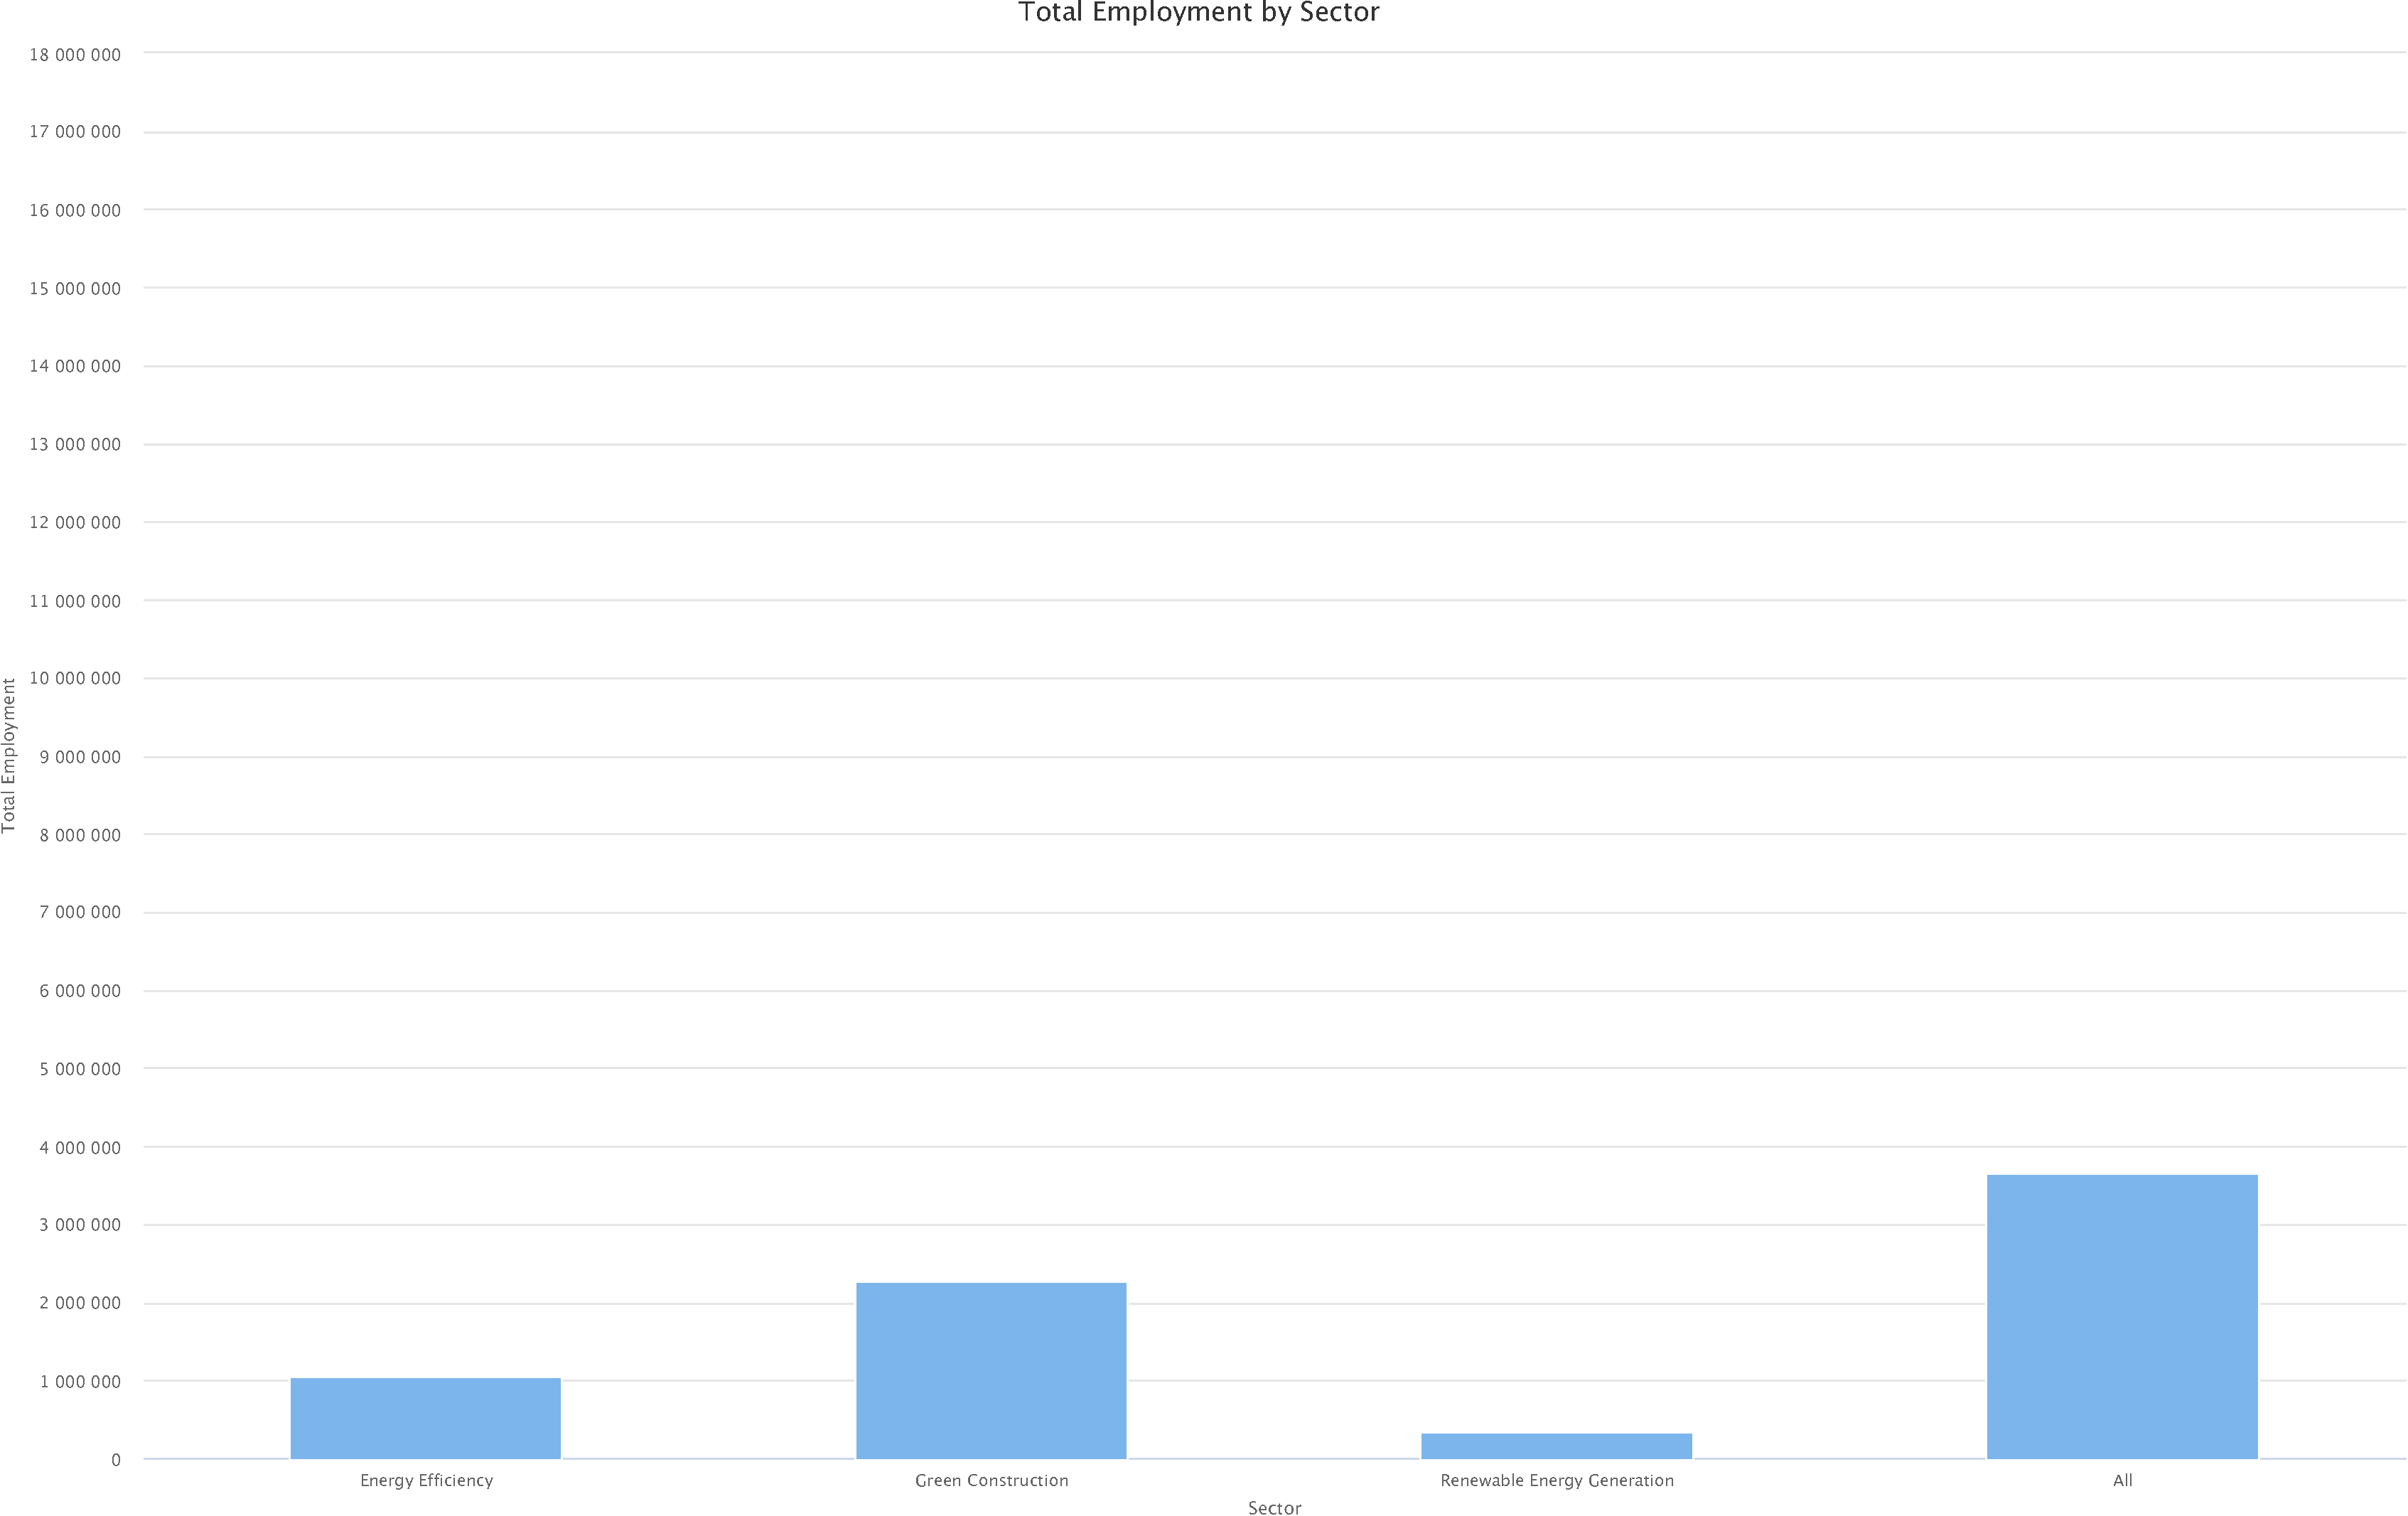
\includegraphics{index_files/figure-pdf/unnamed-chunk-13-1.pdf}

\begin{Shaded}
\begin{Highlighting}[]
\CommentTok{\# Visualizing H\_MEAN (Mean Hourly Wage) across the sectors}
\FunctionTok{hchart}\NormalTok{(final\_summary, }\StringTok{"column"}\NormalTok{, }\FunctionTok{hcaes}\NormalTok{(}\AttributeTok{x =} \StringTok{\textasciigrave{}}\AttributeTok{O*NET{-}SOC Sector}\StringTok{\textasciigrave{}}\NormalTok{, }\AttributeTok{y =}\NormalTok{ H\_MEAN)) }\SpecialCharTok{\%\textgreater{}\%}
  \FunctionTok{hc\_title}\NormalTok{(}\AttributeTok{text =} \StringTok{"Mean Hourly Wage by Sector"}\NormalTok{) }\SpecialCharTok{\%\textgreater{}\%}
  \FunctionTok{hc\_xAxis}\NormalTok{(}\AttributeTok{title =} \FunctionTok{list}\NormalTok{(}\AttributeTok{text =} \StringTok{"Sector"}\NormalTok{)) }\SpecialCharTok{\%\textgreater{}\%}
  \FunctionTok{hc\_yAxis}\NormalTok{(}\AttributeTok{title =} \FunctionTok{list}\NormalTok{(}\AttributeTok{text =} \StringTok{"Mean Hourly Wage (USD)"}\NormalTok{)) }\SpecialCharTok{\%\textgreater{}\%}
  \FunctionTok{hc\_tooltip}\NormalTok{(}\AttributeTok{pointFormat =} \StringTok{\textquotesingle{}\textless{}b\textgreater{}\{point.y:.2f\} USD\textless{}/b\textgreater{}\textquotesingle{}}\NormalTok{)}
\end{Highlighting}
\end{Shaded}

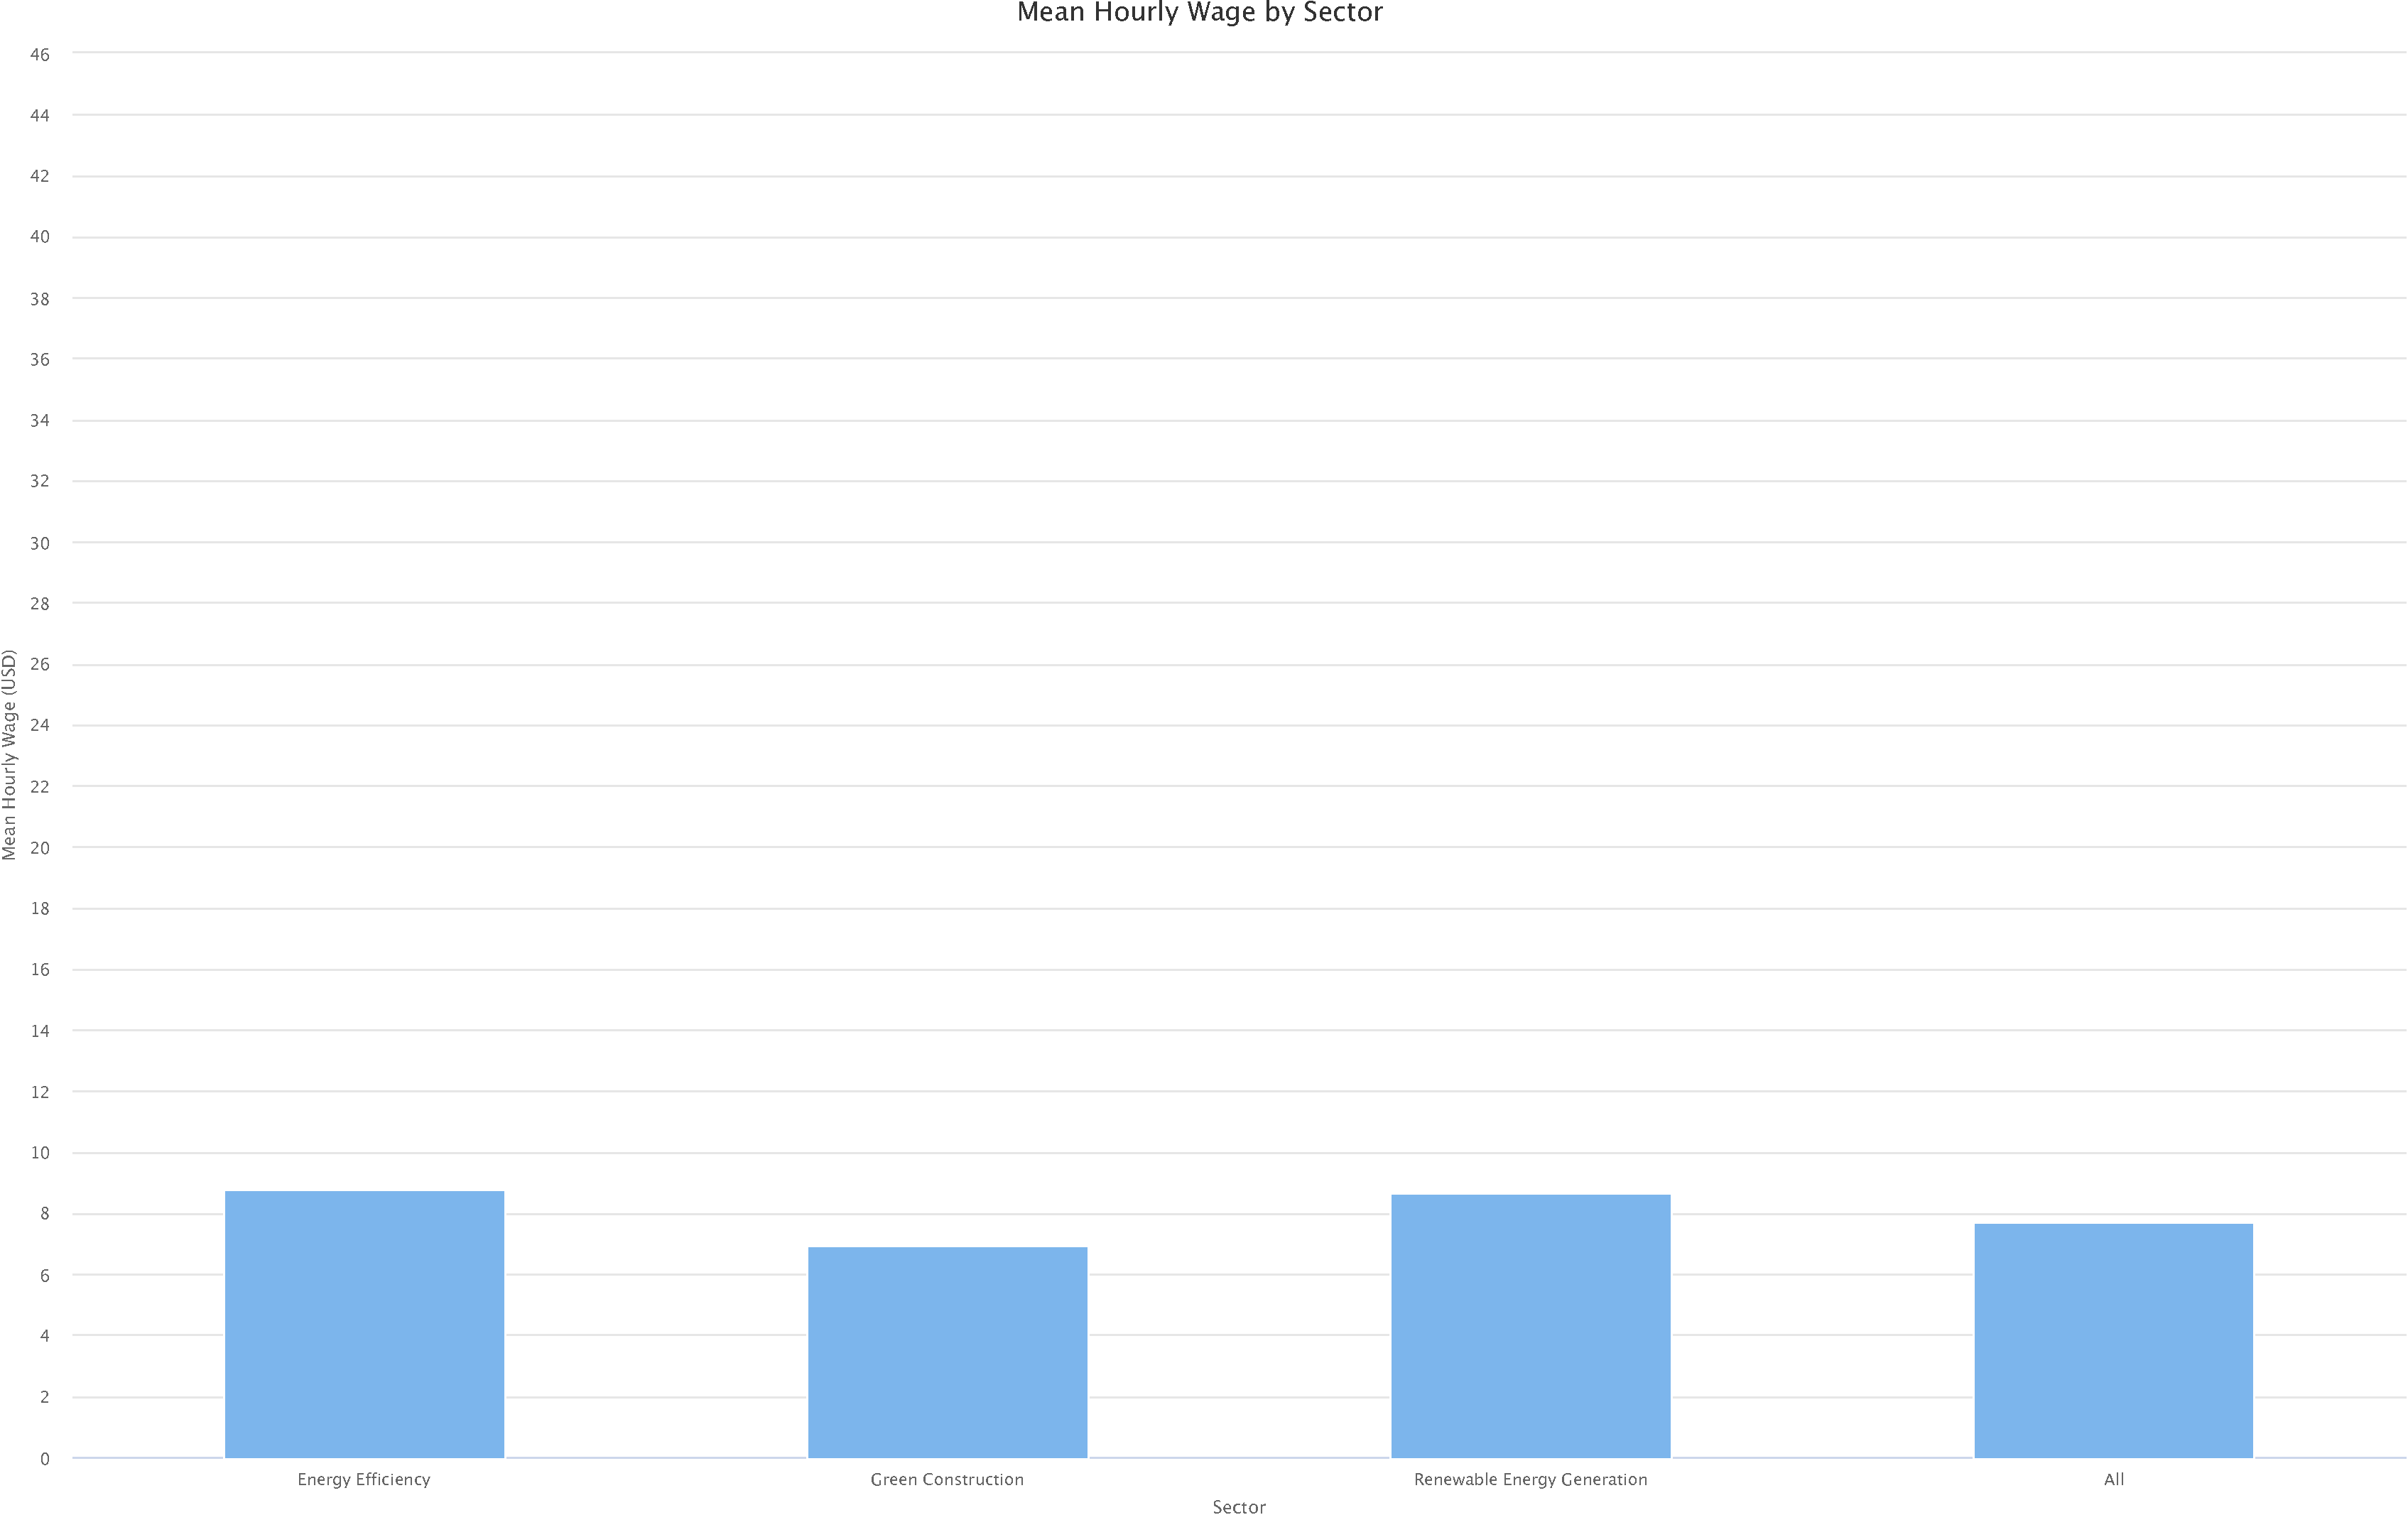
\includegraphics{index_files/figure-pdf/unnamed-chunk-13-2.pdf}

\begin{Shaded}
\begin{Highlighting}[]
\CommentTok{\# Visualizing A\_MEAN (Mean Annual Wage) across the sectors}
\FunctionTok{hchart}\NormalTok{(final\_summary, }\StringTok{"column"}\NormalTok{, }\FunctionTok{hcaes}\NormalTok{(}\AttributeTok{x =} \StringTok{\textasciigrave{}}\AttributeTok{O*NET{-}SOC Sector}\StringTok{\textasciigrave{}}\NormalTok{, }\AttributeTok{y =}\NormalTok{ A\_MEAN)) }\SpecialCharTok{\%\textgreater{}\%}
  \FunctionTok{hc\_title}\NormalTok{(}\AttributeTok{text =} \StringTok{"Mean Annual Wage by Sector"}\NormalTok{) }\SpecialCharTok{\%\textgreater{}\%}
  \FunctionTok{hc\_xAxis}\NormalTok{(}\AttributeTok{title =} \FunctionTok{list}\NormalTok{(}\AttributeTok{text =} \StringTok{"Sector"}\NormalTok{)) }\SpecialCharTok{\%\textgreater{}\%}
  \FunctionTok{hc\_yAxis}\NormalTok{(}\AttributeTok{title =} \FunctionTok{list}\NormalTok{(}\AttributeTok{text =} \StringTok{"Mean Annual Wage (USD)"}\NormalTok{), }\AttributeTok{labels =} \FunctionTok{list}\NormalTok{(}\AttributeTok{format =} \StringTok{"\{value:,0f\}"}\NormalTok{)) }\SpecialCharTok{\%\textgreater{}\%}
  \FunctionTok{hc\_tooltip}\NormalTok{(}\AttributeTok{pointFormat =} \StringTok{\textquotesingle{}\textless{}b\textgreater{}\{point.y:,0f\} USD\textless{}/b\textgreater{}\textquotesingle{}}\NormalTok{)}
\end{Highlighting}
\end{Shaded}

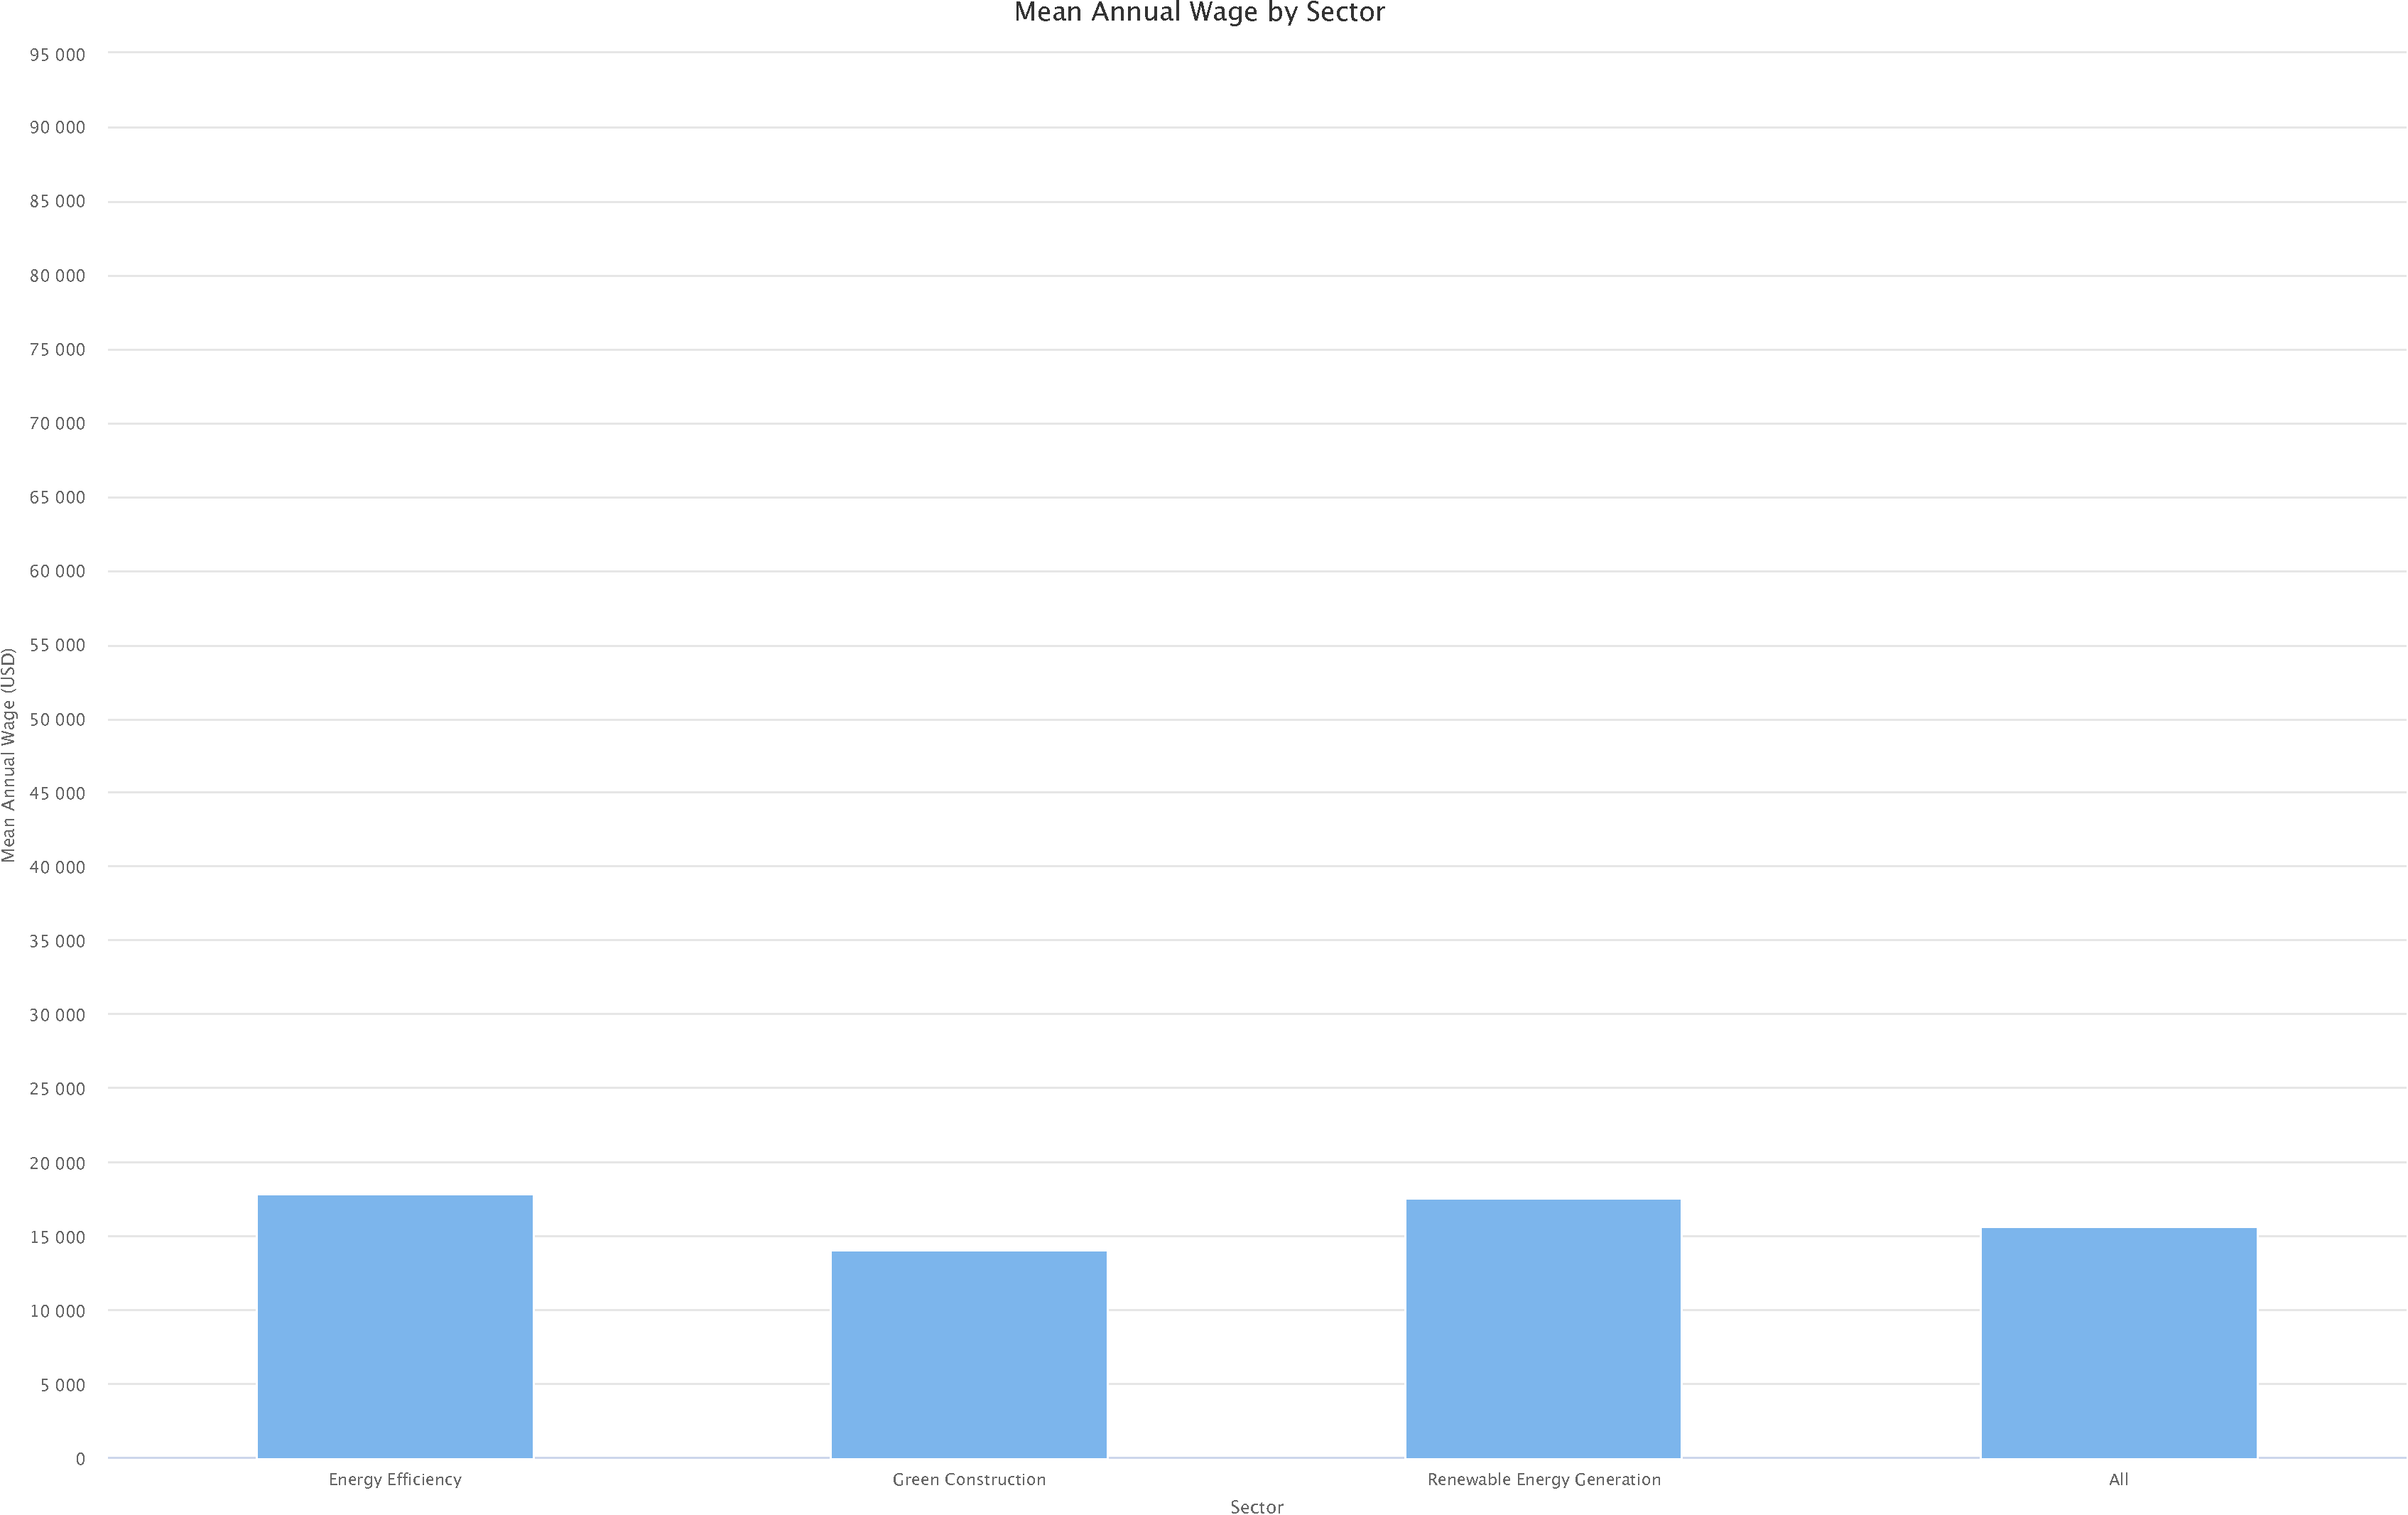
\includegraphics{index_files/figure-pdf/unnamed-chunk-13-3.pdf}

\begin{Shaded}
\begin{Highlighting}[]
\CommentTok{\# Visualizing A\_MEDIAN (Median Annual Wage) across the sectors}
\FunctionTok{hchart}\NormalTok{(final\_summary, }\StringTok{"column"}\NormalTok{, }\FunctionTok{hcaes}\NormalTok{(}\AttributeTok{x =} \StringTok{\textasciigrave{}}\AttributeTok{O*NET{-}SOC Sector}\StringTok{\textasciigrave{}}\NormalTok{, }\AttributeTok{y =}\NormalTok{ A\_MEDIAN)) }\SpecialCharTok{\%\textgreater{}\%}
  \FunctionTok{hc\_title}\NormalTok{(}\AttributeTok{text =} \StringTok{"Median Annual Wage by Sector"}\NormalTok{) }\SpecialCharTok{\%\textgreater{}\%}
  \FunctionTok{hc\_xAxis}\NormalTok{(}\AttributeTok{title =} \FunctionTok{list}\NormalTok{(}\AttributeTok{text =} \StringTok{"Sector"}\NormalTok{)) }\SpecialCharTok{\%\textgreater{}\%}
  \FunctionTok{hc\_yAxis}\NormalTok{(}\AttributeTok{title =} \FunctionTok{list}\NormalTok{(}\AttributeTok{text =} \StringTok{"Median Annual Wage (USD)"}\NormalTok{), }\AttributeTok{labels =} \FunctionTok{list}\NormalTok{(}\AttributeTok{format =} \StringTok{"\{value:,0f\}"}\NormalTok{)) }\SpecialCharTok{\%\textgreater{}\%}
  \FunctionTok{hc\_tooltip}\NormalTok{(}\AttributeTok{pointFormat =} \StringTok{\textquotesingle{}\textless{}b\textgreater{}\{point.y:,0f\} USD\textless{}/b\textgreater{}\textquotesingle{}}\NormalTok{)}
\end{Highlighting}
\end{Shaded}

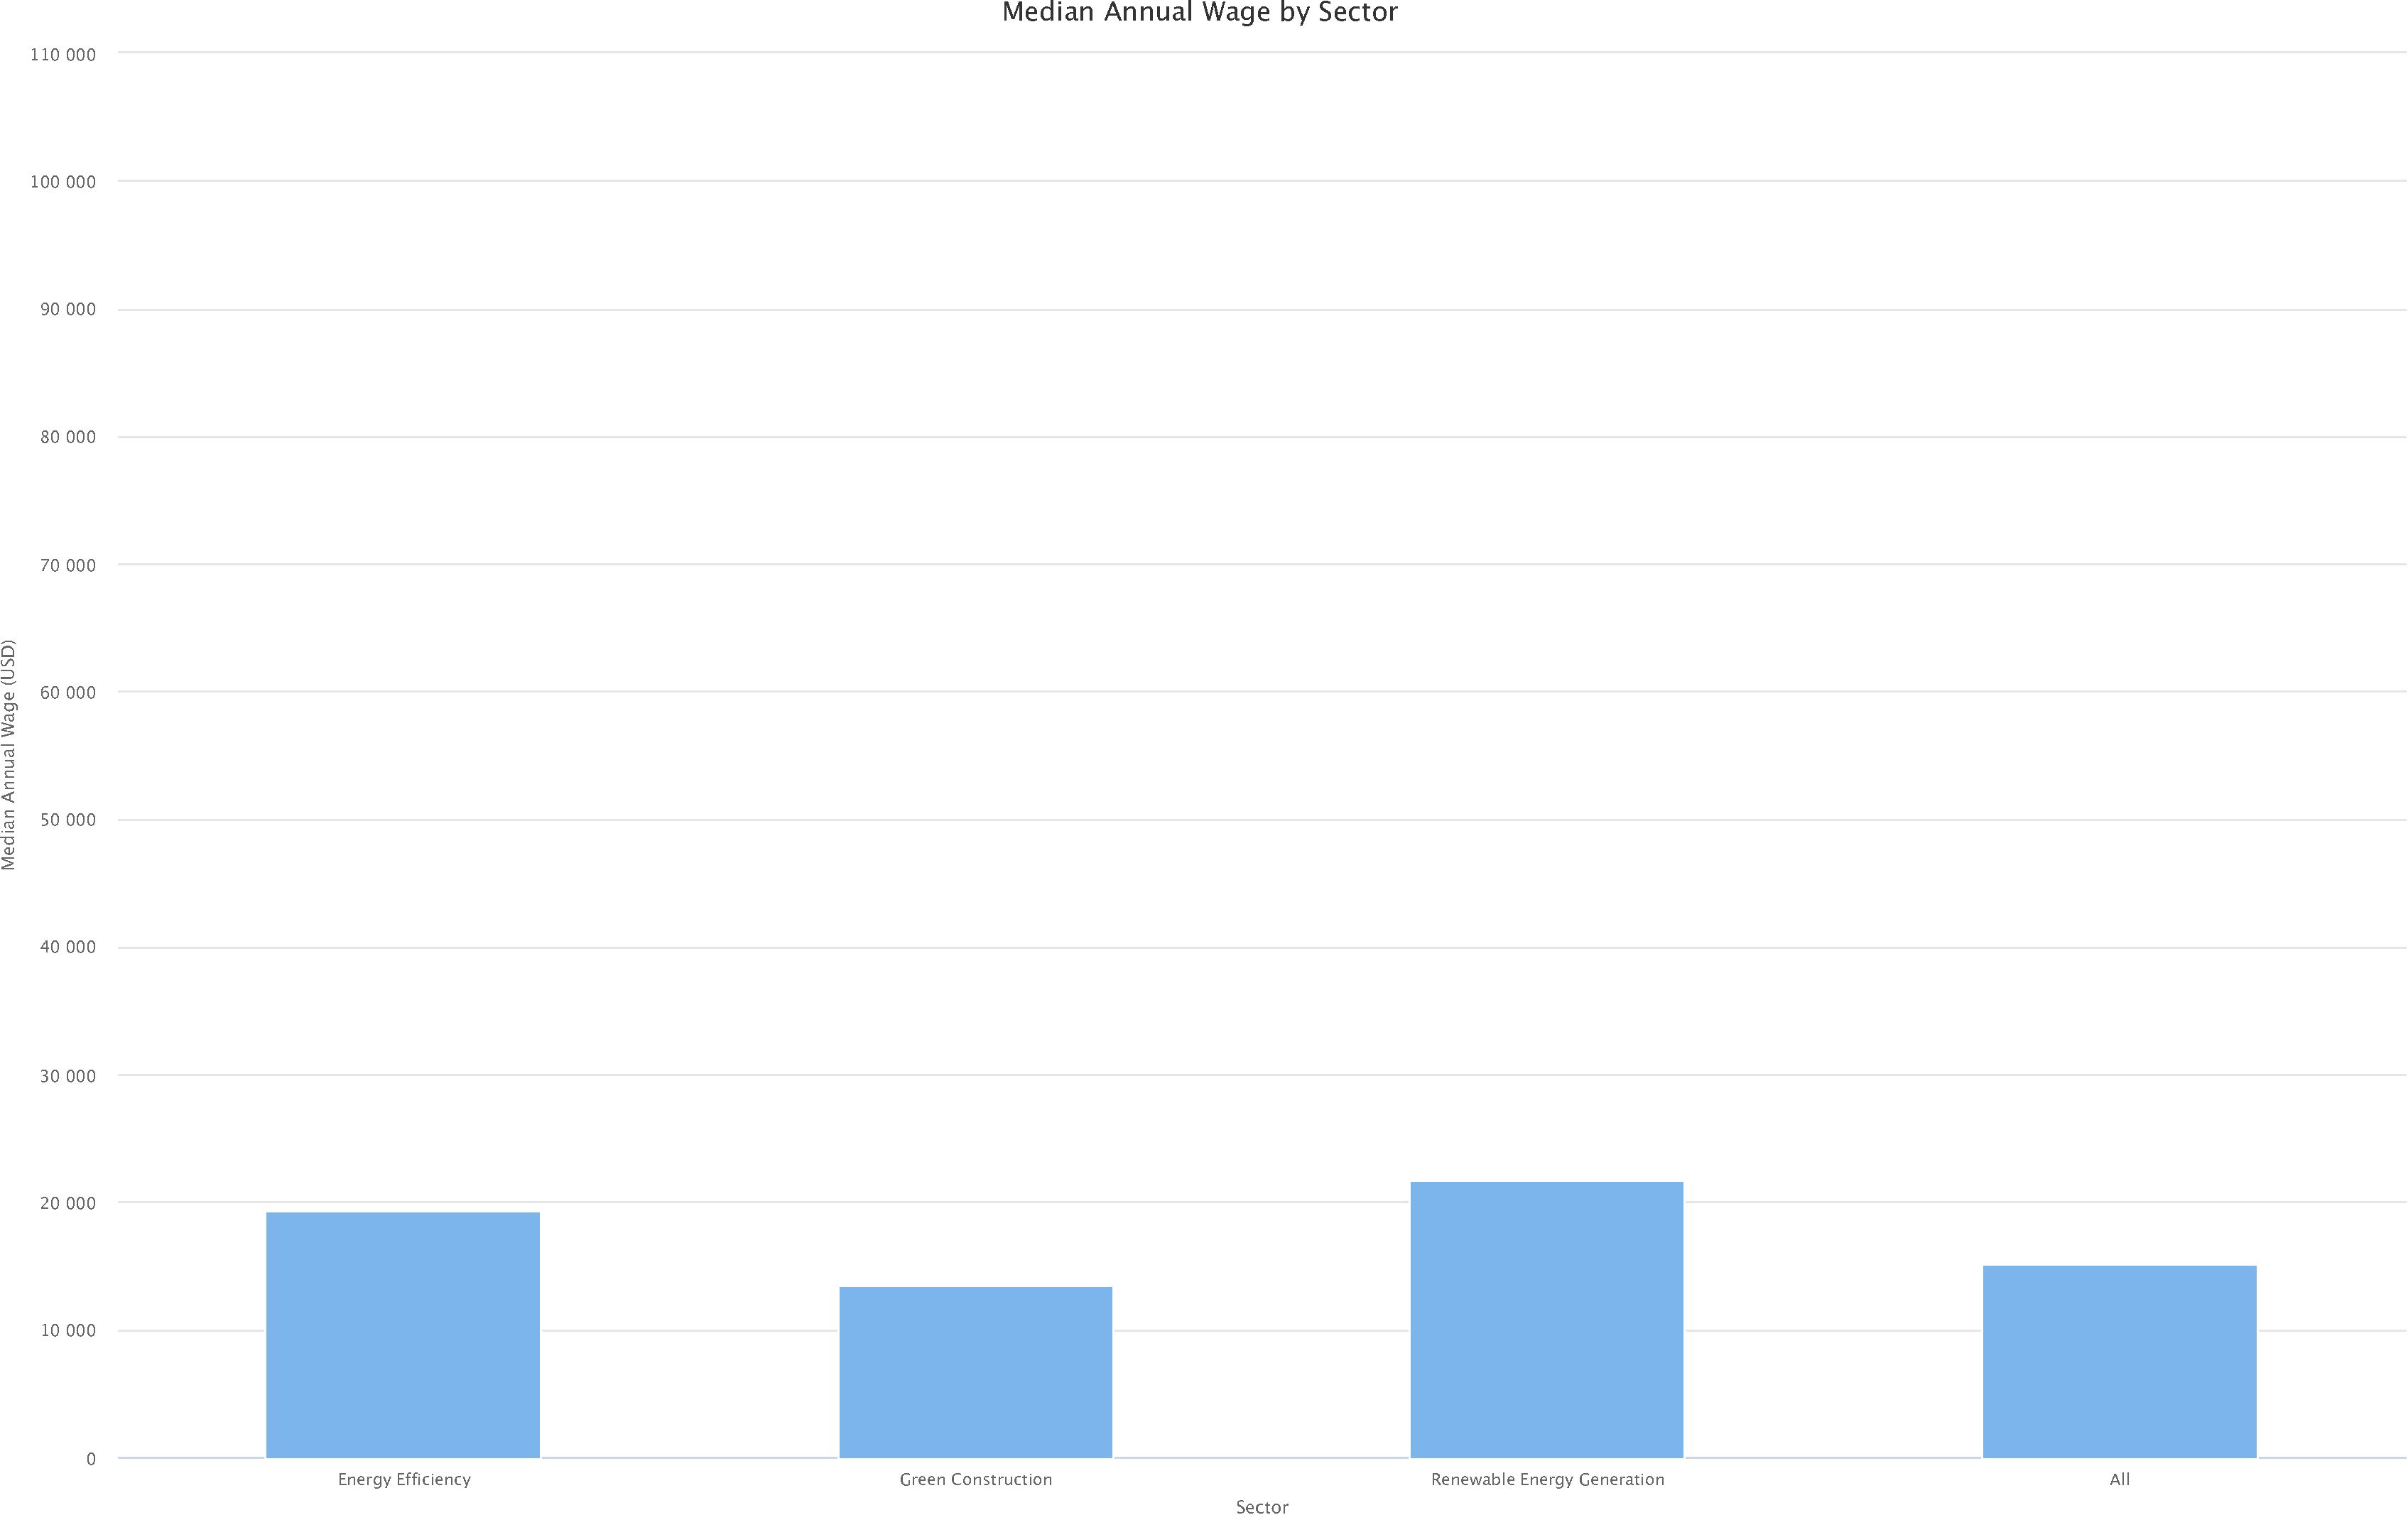
\includegraphics{index_files/figure-pdf/unnamed-chunk-13-4.pdf}

\begin{Shaded}
\begin{Highlighting}[]
\CommentTok{\# Visualizing H\_MEDIAN (Median Hourly Wage) across the sectors}
\FunctionTok{hchart}\NormalTok{(final\_summary, }\StringTok{"column"}\NormalTok{, }\FunctionTok{hcaes}\NormalTok{(}\AttributeTok{x =} \StringTok{\textasciigrave{}}\AttributeTok{O*NET{-}SOC Sector}\StringTok{\textasciigrave{}}\NormalTok{, }\AttributeTok{y =}\NormalTok{ H\_MEDIAN)) }\SpecialCharTok{\%\textgreater{}\%}
  \FunctionTok{hc\_title}\NormalTok{(}\AttributeTok{text =} \StringTok{"Median Hourly Wage by Sector"}\NormalTok{) }\SpecialCharTok{\%\textgreater{}\%}
  \FunctionTok{hc\_xAxis}\NormalTok{(}\AttributeTok{title =} \FunctionTok{list}\NormalTok{(}\AttributeTok{text =} \StringTok{"Sector"}\NormalTok{)) }\SpecialCharTok{\%\textgreater{}\%}
  \FunctionTok{hc\_yAxis}\NormalTok{(}\AttributeTok{title =} \FunctionTok{list}\NormalTok{(}\AttributeTok{text =} \StringTok{"Median Hourly Wage (USD)"}\NormalTok{)) }\SpecialCharTok{\%\textgreater{}\%}
  \FunctionTok{hc\_tooltip}\NormalTok{(}\AttributeTok{pointFormat =} \StringTok{\textquotesingle{}\textless{}b\textgreater{}\{point.y:.2f\} USD\textless{}/b\textgreater{}\textquotesingle{}}\NormalTok{)}
\end{Highlighting}
\end{Shaded}

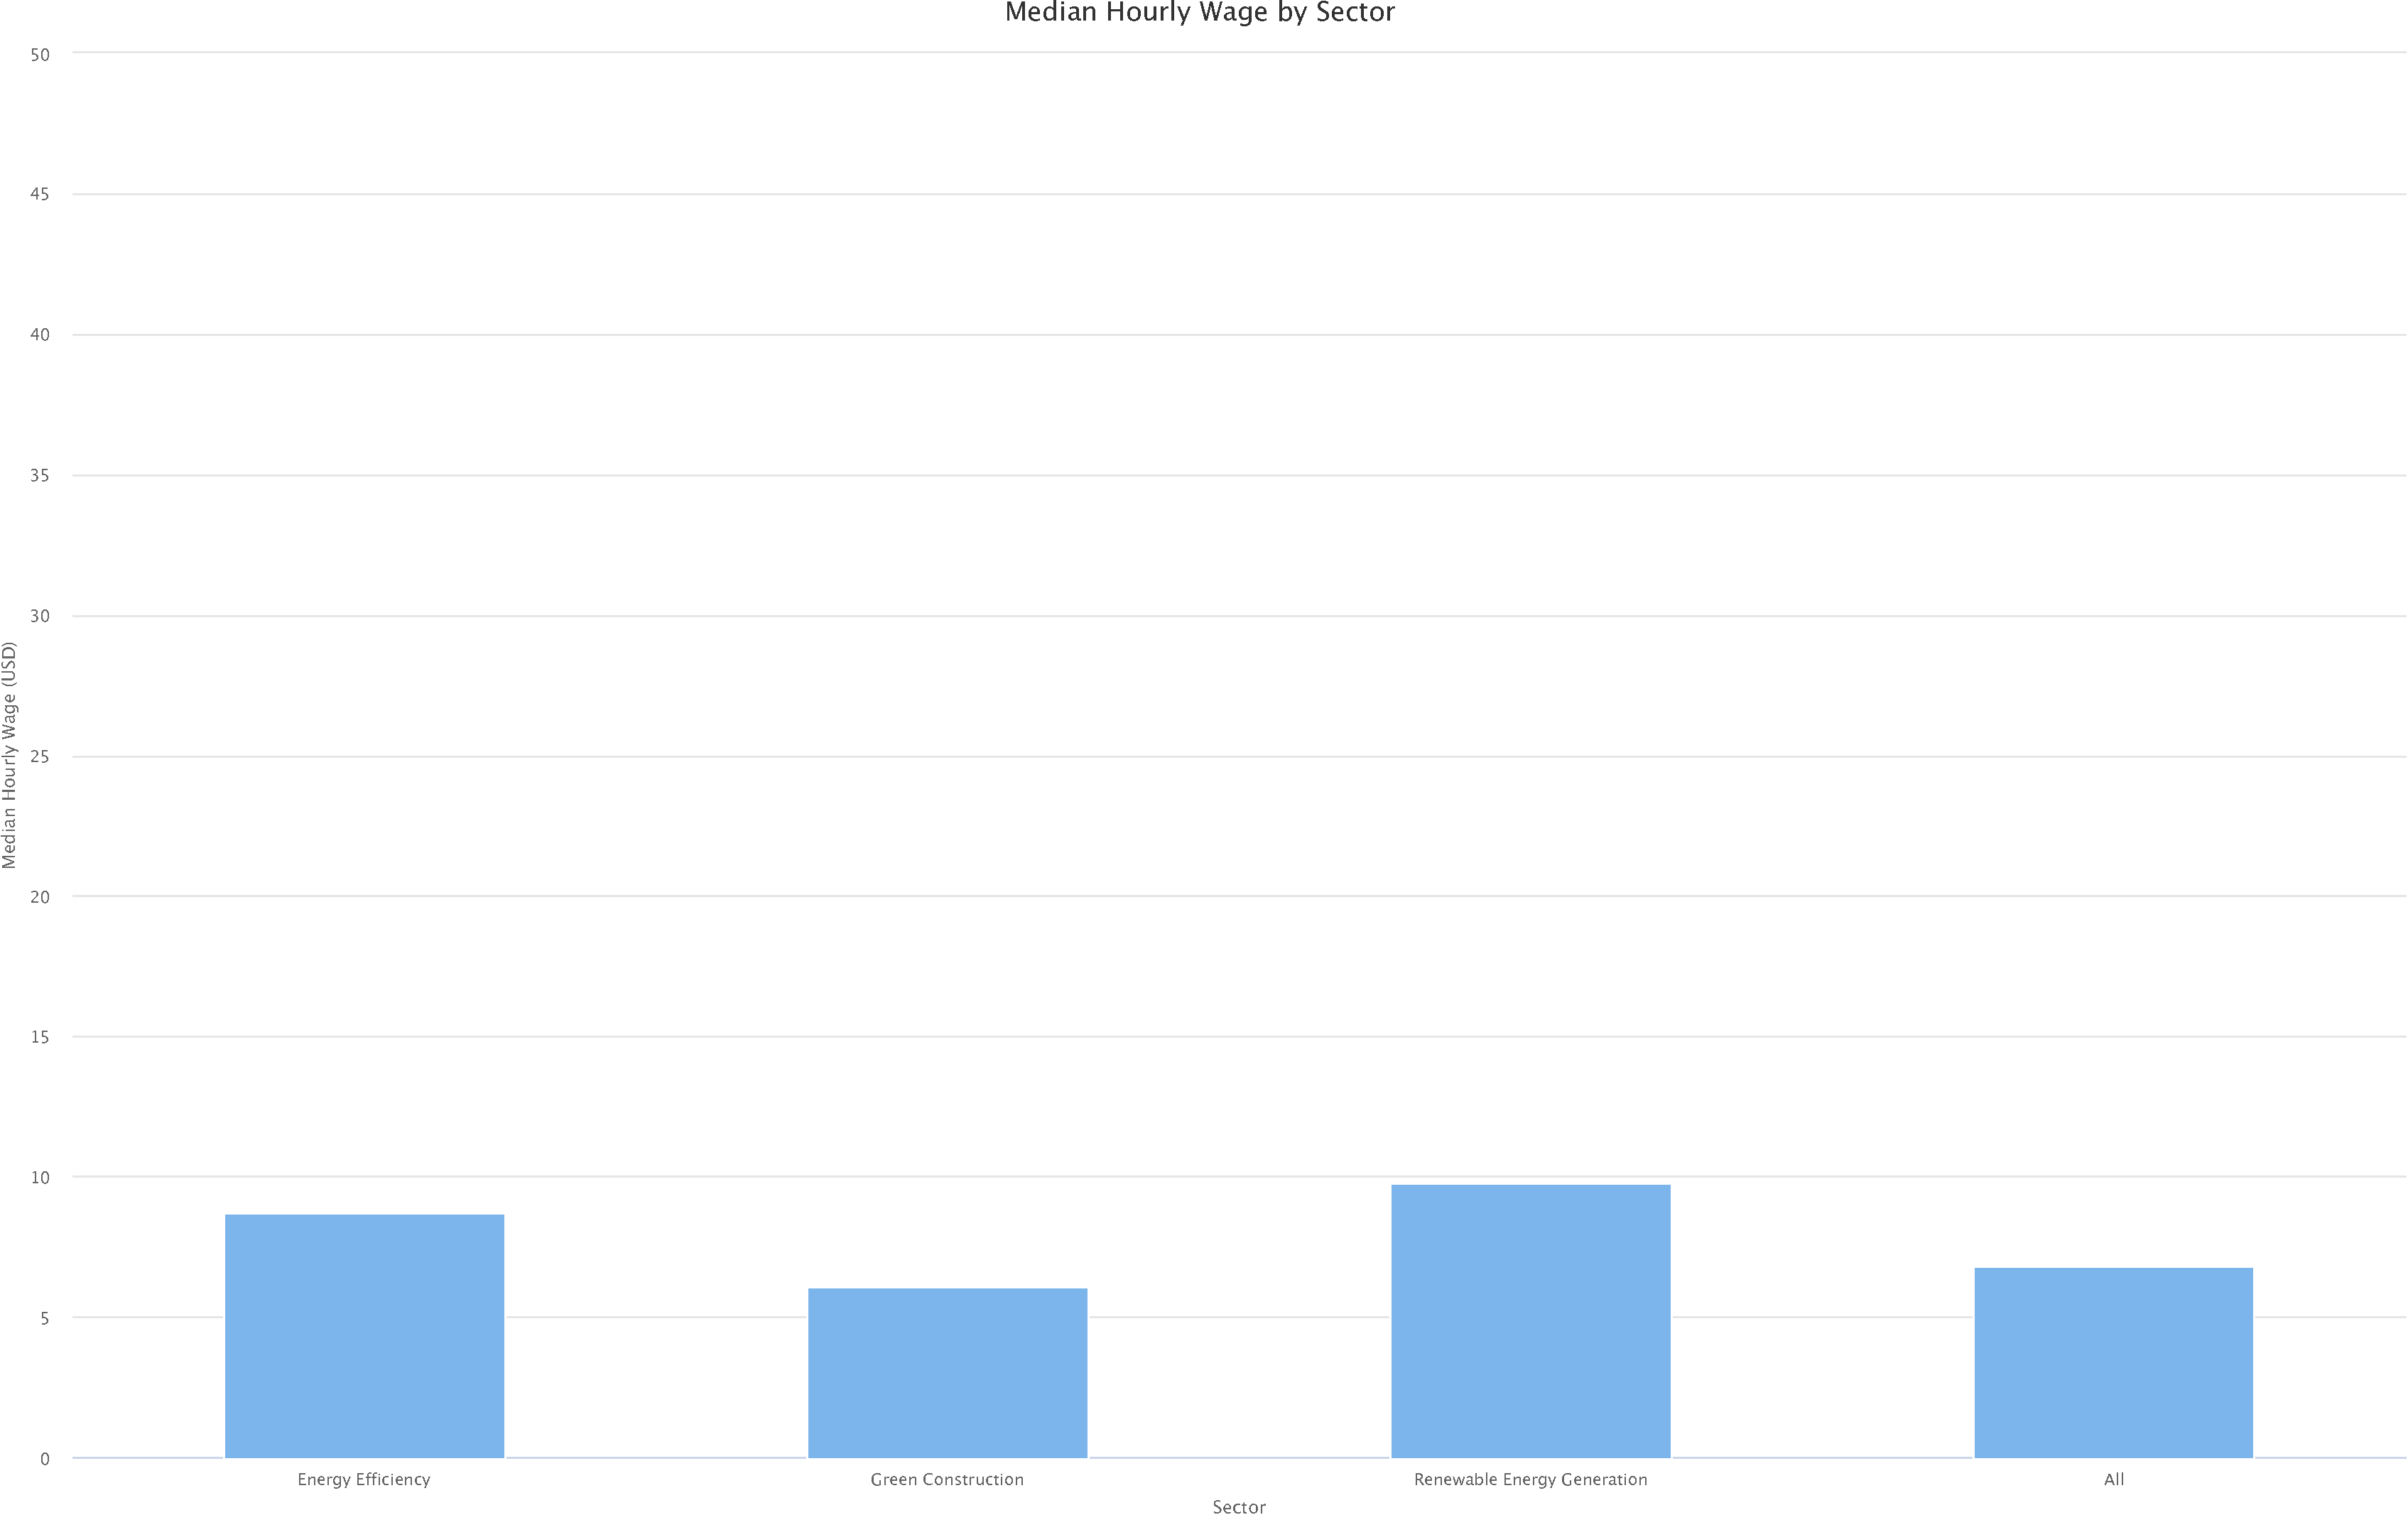
\includegraphics{index_files/figure-pdf/unnamed-chunk-13-5.pdf}

\textsubscript{Source:
\href{https://beeckcenter.github.io/climate-equity-workforce/index-preview.html}{Article
Notebook}}

I'm also curious about the differences between green jobs and non-green
jobs for mean hourly wage and mean annual wage.

\begin{Shaded}
\begin{Highlighting}[]
\CommentTok{\# Define green jobs as sectors related to energy and construction}
\NormalTok{green\_jobs\_sectors }\OtherTok{\textless{}{-}} \FunctionTok{c}\NormalTok{(}\StringTok{"Energy Efficiency"}\NormalTok{, }\StringTok{"Renewable Energy Generation"}\NormalTok{, }\StringTok{"Green Construction"}\NormalTok{)}

\CommentTok{\# Add a new column to identify green and non{-}green jobs}
\NormalTok{national\_jobs }\OtherTok{\textless{}{-}}\NormalTok{ national\_jobs }\SpecialCharTok{\%\textgreater{}\%}
  \FunctionTok{mutate}\NormalTok{(}
    \AttributeTok{Job\_Type =} \FunctionTok{ifelse}\NormalTok{(}\StringTok{\textasciigrave{}}\AttributeTok{O*NET{-}SOC Sector}\StringTok{\textasciigrave{}} \SpecialCharTok{\%in\%}\NormalTok{ green\_jobs\_sectors, }\StringTok{"Green Jobs"}\NormalTok{, }\StringTok{"Non{-}Green Jobs"}\NormalTok{)}
\NormalTok{  )}

\CommentTok{\# Group by job type (Green vs Non{-}Green) and calculate mean wages}
\NormalTok{job\_type\_summary }\OtherTok{\textless{}{-}}\NormalTok{ national\_jobs }\SpecialCharTok{\%\textgreater{}\%}
  \FunctionTok{group\_by}\NormalTok{(Job\_Type) }\SpecialCharTok{\%\textgreater{}\%}
  \FunctionTok{summarize}\NormalTok{(}
    \AttributeTok{H\_MEAN =} \FunctionTok{mean}\NormalTok{(H\_MEAN, }\AttributeTok{na.rm =} \ConstantTok{TRUE}\NormalTok{),}
    \AttributeTok{A\_MEAN =} \FunctionTok{mean}\NormalTok{(A\_MEAN, }\AttributeTok{na.rm =} \ConstantTok{TRUE}\NormalTok{)}
\NormalTok{  )}

\CommentTok{\# Visualizing Mean Hourly Wage (H\_MEAN) for Green vs Non{-}Green Jobs}
\FunctionTok{hchart}\NormalTok{(job\_type\_summary, }\StringTok{"column"}\NormalTok{, }\FunctionTok{hcaes}\NormalTok{(}\AttributeTok{x =}\NormalTok{ Job\_Type, }\AttributeTok{y =}\NormalTok{ H\_MEAN)) }\SpecialCharTok{\%\textgreater{}\%}
  \FunctionTok{hc\_title}\NormalTok{(}\AttributeTok{text =} \StringTok{"Mean Hourly Wage: Green Jobs vs Non{-}Green Jobs"}\NormalTok{) }\SpecialCharTok{\%\textgreater{}\%}
  \FunctionTok{hc\_xAxis}\NormalTok{(}\AttributeTok{title =} \FunctionTok{list}\NormalTok{(}\AttributeTok{text =} \StringTok{"Job Type"}\NormalTok{)) }\SpecialCharTok{\%\textgreater{}\%}
  \FunctionTok{hc\_yAxis}\NormalTok{(}\AttributeTok{title =} \FunctionTok{list}\NormalTok{(}\AttributeTok{text =} \StringTok{"Mean Hourly Wage (USD)"}\NormalTok{)) }\SpecialCharTok{\%\textgreater{}\%}
  \FunctionTok{hc\_tooltip}\NormalTok{(}\AttributeTok{pointFormat =} \StringTok{\textquotesingle{}\textless{}b\textgreater{}\{point.y:.2f\} USD\textless{}/b\textgreater{}\textquotesingle{}}\NormalTok{)}
\end{Highlighting}
\end{Shaded}

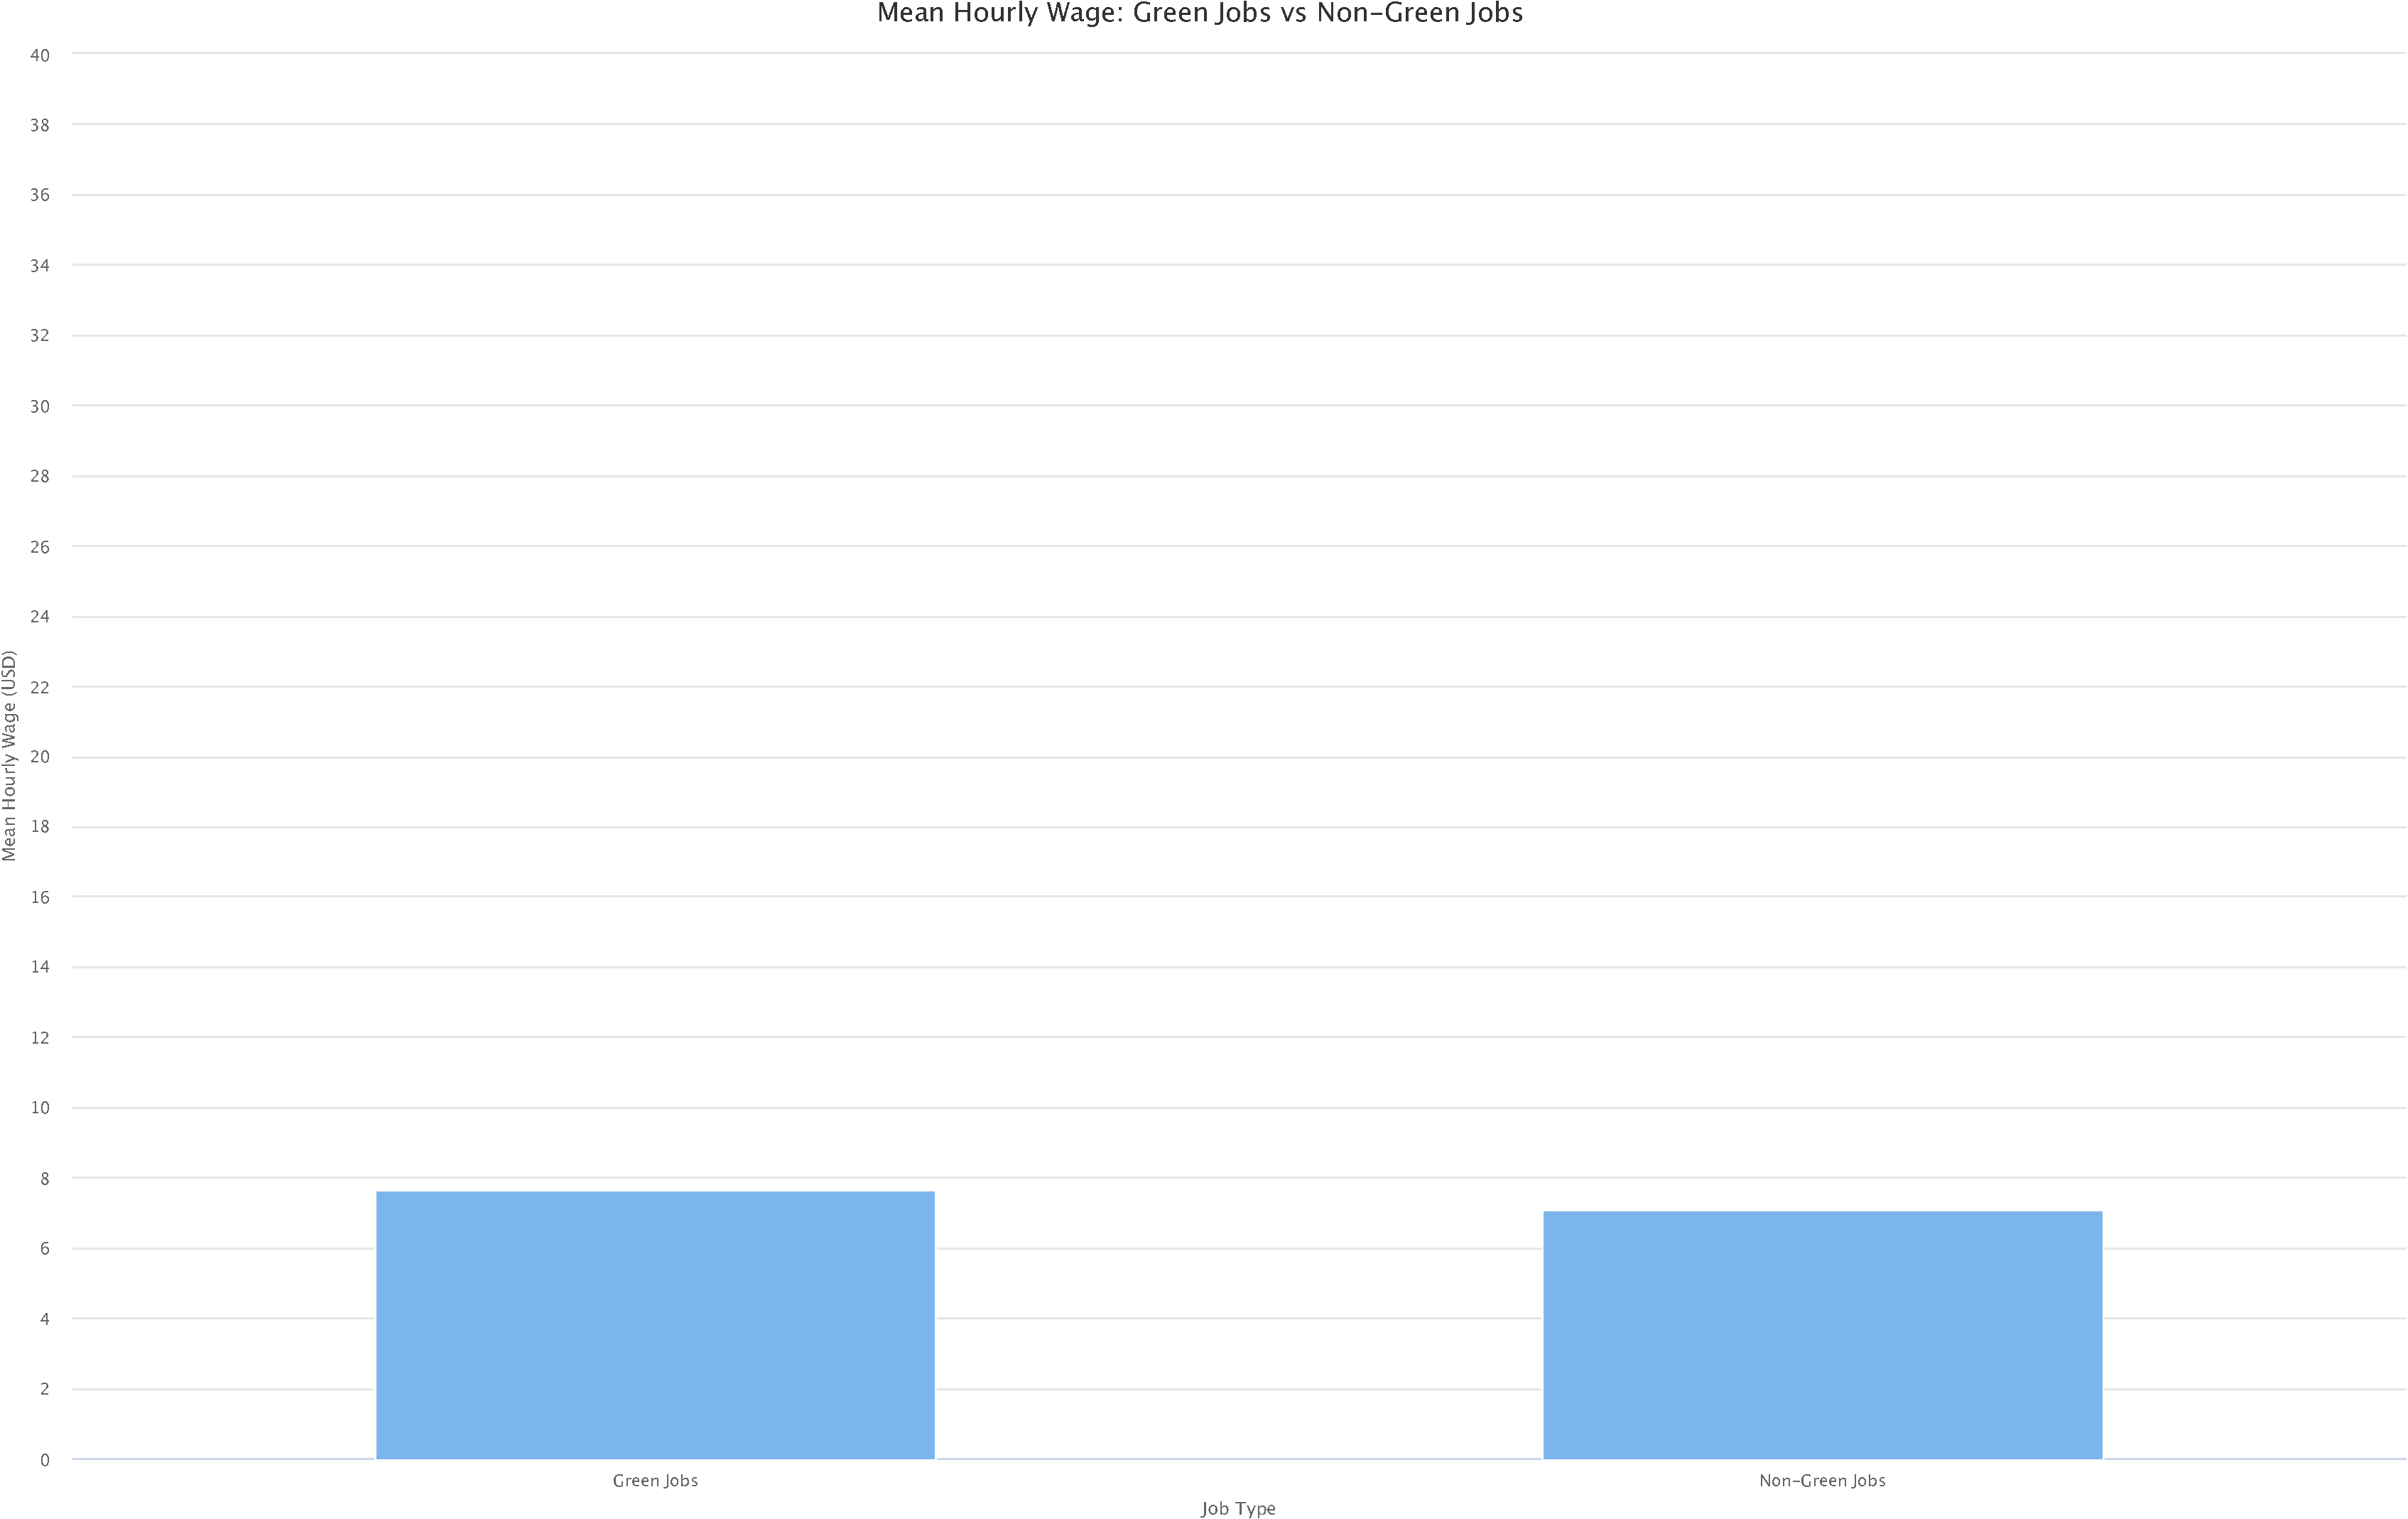
\includegraphics{index_files/figure-pdf/unnamed-chunk-14-1.pdf}

\begin{Shaded}
\begin{Highlighting}[]
\CommentTok{\# Visualizing Mean Annual Wage (A\_MEAN) for Green vs Non{-}Green Jobs}
\FunctionTok{hchart}\NormalTok{(job\_type\_summary, }\StringTok{"column"}\NormalTok{, }\FunctionTok{hcaes}\NormalTok{(}\AttributeTok{x =}\NormalTok{ Job\_Type, }\AttributeTok{y =}\NormalTok{ A\_MEAN)) }\SpecialCharTok{\%\textgreater{}\%}
  \FunctionTok{hc\_title}\NormalTok{(}\AttributeTok{text =} \StringTok{"Mean Annual Wage: Green Jobs vs Non{-}Green Jobs"}\NormalTok{) }\SpecialCharTok{\%\textgreater{}\%}
  \FunctionTok{hc\_xAxis}\NormalTok{(}\AttributeTok{title =} \FunctionTok{list}\NormalTok{(}\AttributeTok{text =} \StringTok{"Job Type"}\NormalTok{)) }\SpecialCharTok{\%\textgreater{}\%}
  \FunctionTok{hc\_yAxis}\NormalTok{(}\AttributeTok{title =} \FunctionTok{list}\NormalTok{(}\AttributeTok{text =} \StringTok{"Mean Annual Wage (USD)"}\NormalTok{)) }\SpecialCharTok{\%\textgreater{}\%}
  \FunctionTok{hc\_tooltip}\NormalTok{(}\AttributeTok{pointFormat =} \StringTok{\textquotesingle{}\textless{}b\textgreater{}\{point.y:,0f\} USD\textless{}/b\textgreater{}\textquotesingle{}}\NormalTok{)}
\end{Highlighting}
\end{Shaded}

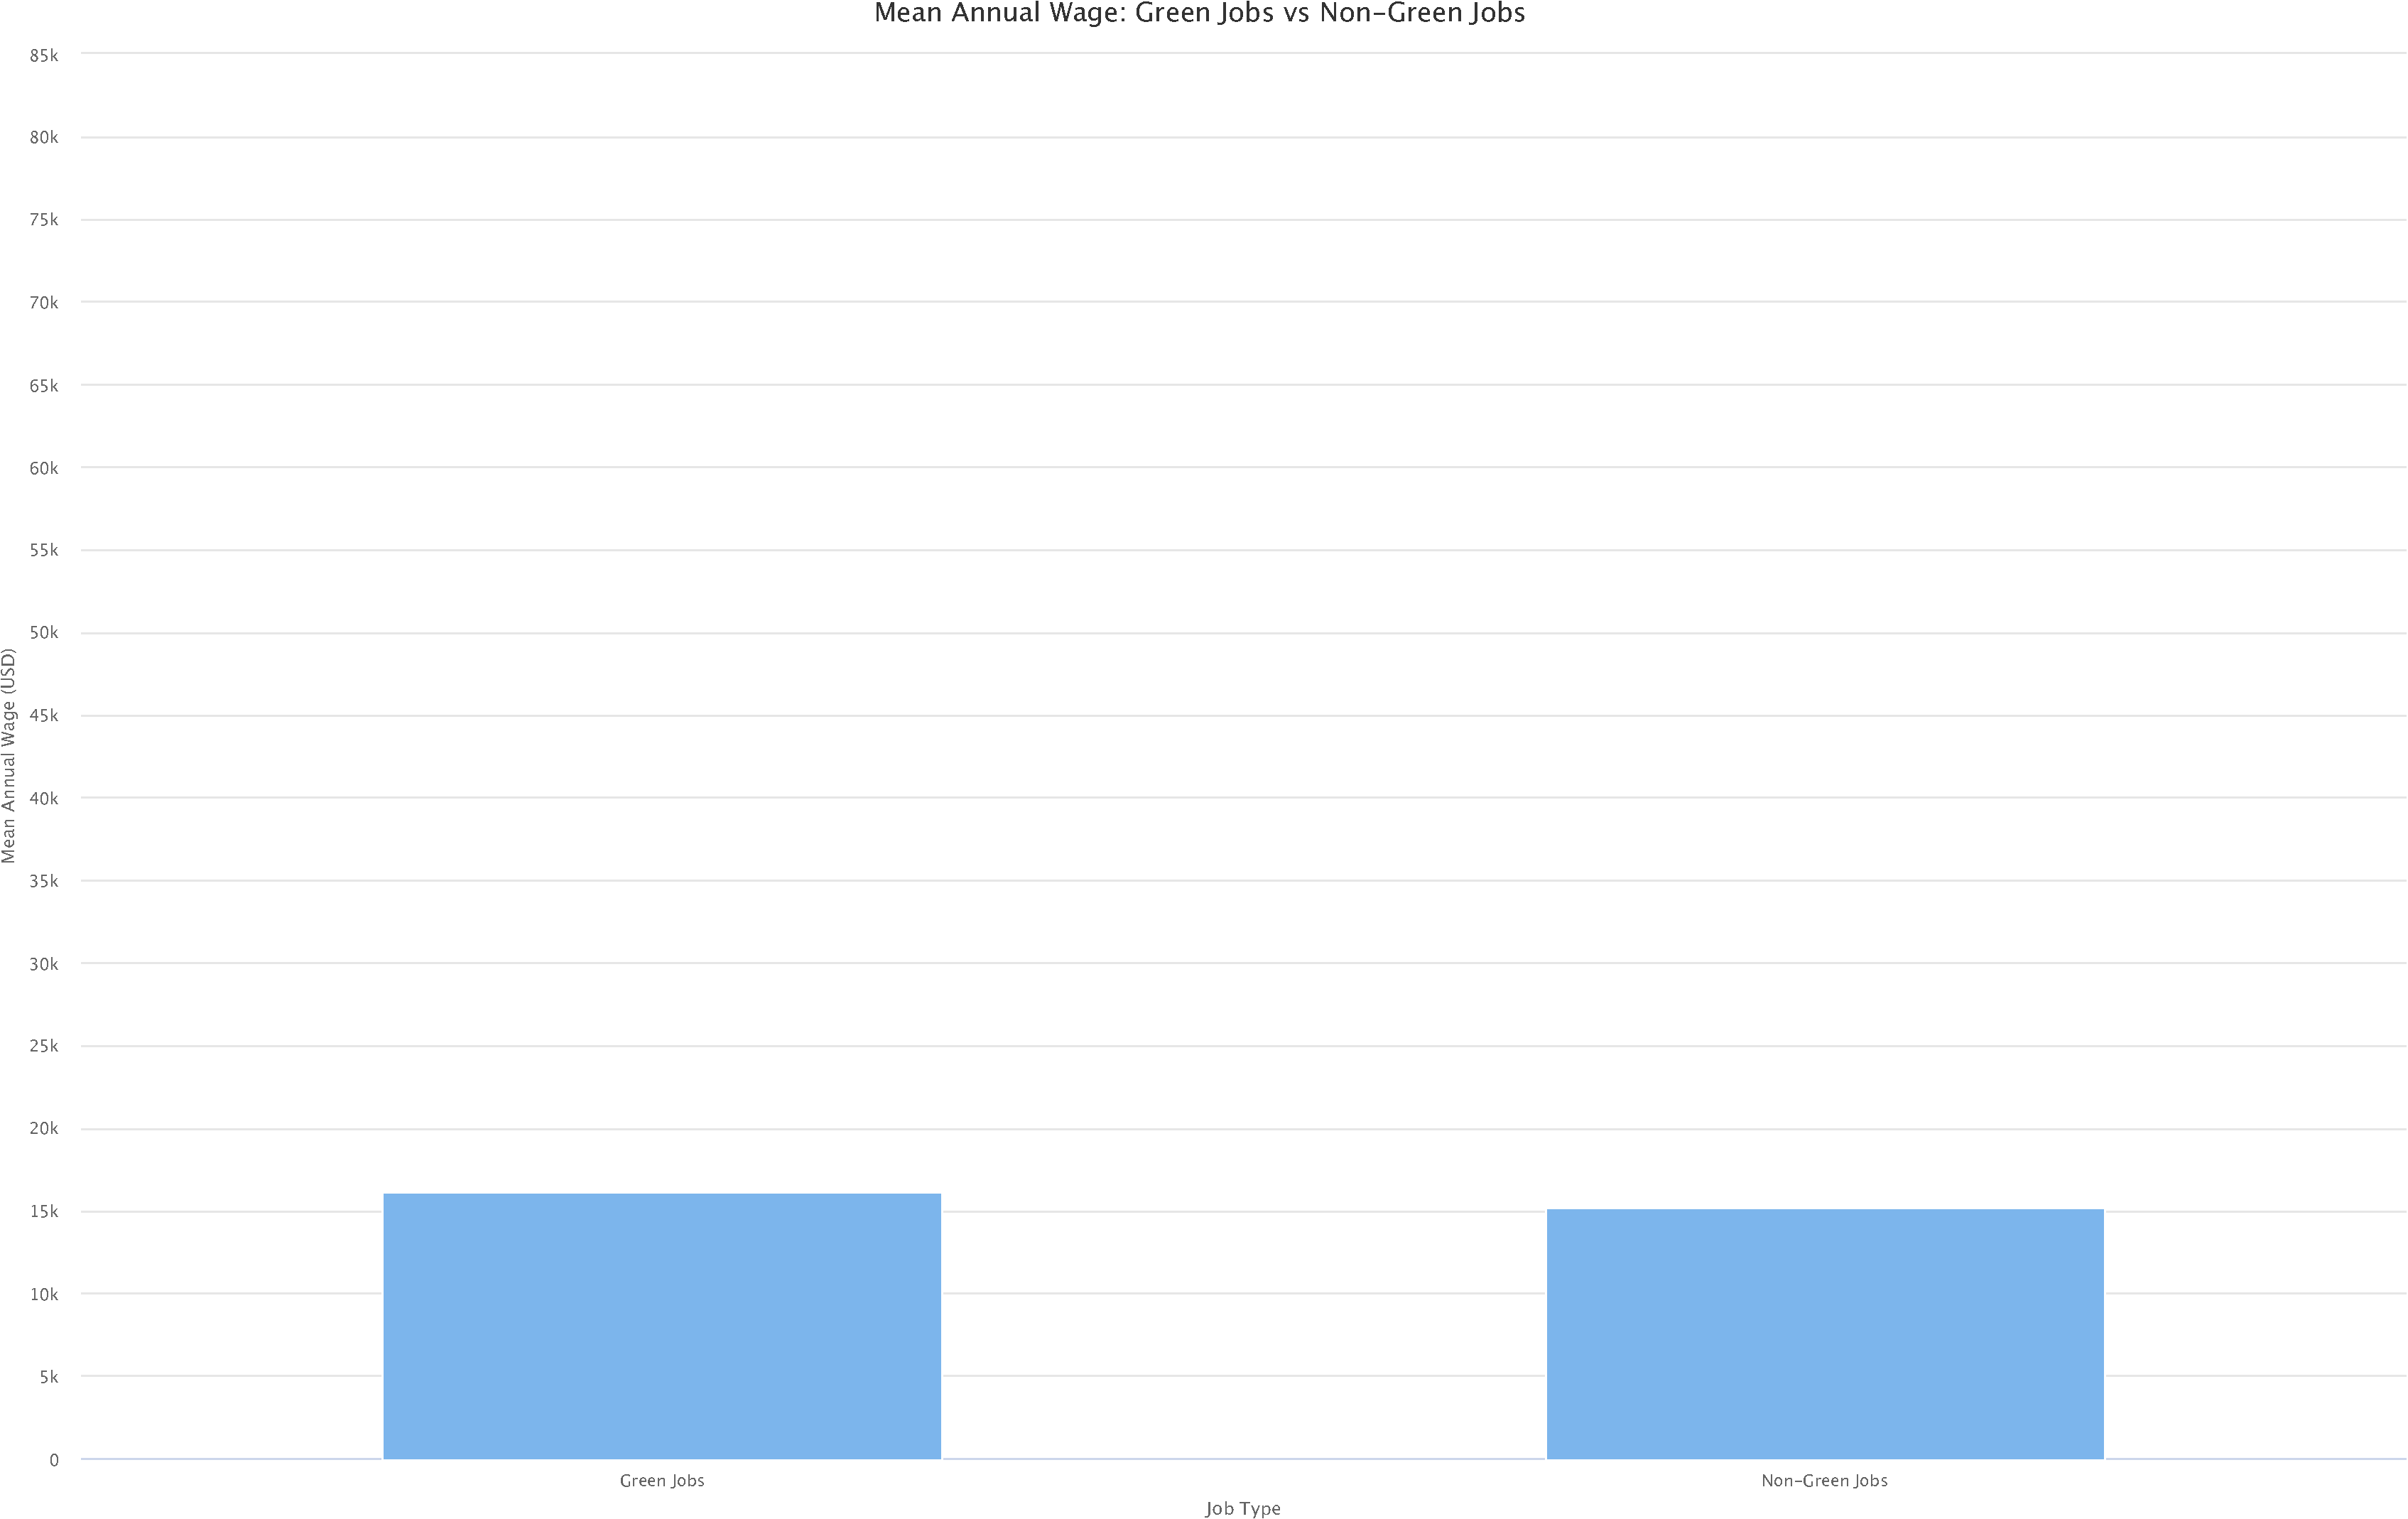
\includegraphics{index_files/figure-pdf/unnamed-chunk-14-2.pdf}

\textsubscript{Source:
\href{https://beeckcenter.github.io/climate-equity-workforce/index-preview.html}{Article
Notebook}}

\begin{Shaded}
\begin{Highlighting}[]
\CommentTok{\# Summarizing core findings nationally}

\CommentTok{\# Extract green and non{-}green job wage data}
\NormalTok{green\_wages }\OtherTok{\textless{}{-}}\NormalTok{ job\_type\_summary }\SpecialCharTok{\%\textgreater{}\%} \FunctionTok{filter}\NormalTok{(Job\_Type }\SpecialCharTok{==} \StringTok{"Green Jobs"}\NormalTok{)}
\NormalTok{non\_green\_wages }\OtherTok{\textless{}{-}}\NormalTok{ job\_type\_summary }\SpecialCharTok{\%\textgreater{}\%} \FunctionTok{filter}\NormalTok{(Job\_Type }\SpecialCharTok{==} \StringTok{"Non{-}Green Jobs"}\NormalTok{)}

\CommentTok{\# Calculate the difference between green and non{-}green jobs}
\NormalTok{difference\_annual }\OtherTok{\textless{}{-}}\NormalTok{ green\_wages}\SpecialCharTok{$}\NormalTok{A\_MEAN }\SpecialCharTok{{-}}\NormalTok{ non\_green\_wages}\SpecialCharTok{$}\NormalTok{A\_MEAN}
\NormalTok{difference\_hourly }\OtherTok{\textless{}{-}}\NormalTok{ green\_wages}\SpecialCharTok{$}\NormalTok{H\_MEAN }\SpecialCharTok{{-}}\NormalTok{ non\_green\_wages}\SpecialCharTok{$}\NormalTok{H\_MEAN}

\CommentTok{\# Format and print the sentences}
\FunctionTok{cat}\NormalTok{(}\StringTok{"The mean annual wage for the occupation in U.S. dollars for green jobs is $"}\NormalTok{, }
    \FunctionTok{format}\NormalTok{(green\_wages}\SpecialCharTok{$}\NormalTok{A\_MEAN, }\AttributeTok{big.mark =} \StringTok{","}\NormalTok{, }\AttributeTok{scientific =} \ConstantTok{FALSE}\NormalTok{), }
    \StringTok{", and for non{-}green jobs is $"}\NormalTok{, }
    \FunctionTok{format}\NormalTok{(non\_green\_wages}\SpecialCharTok{$}\NormalTok{A\_MEAN, }\AttributeTok{big.mark =} \StringTok{","}\NormalTok{, }\AttributeTok{scientific =} \ConstantTok{FALSE}\NormalTok{), }
    \StringTok{". That means green jobs pay $"}\NormalTok{, }
    \FunctionTok{format}\NormalTok{(}\FunctionTok{abs}\NormalTok{(difference\_annual), }\AttributeTok{big.mark =} \StringTok{","}\NormalTok{, }\AttributeTok{scientific =} \ConstantTok{FALSE}\NormalTok{), }
    \FunctionTok{ifelse}\NormalTok{(difference\_annual }\SpecialCharTok{\textgreater{}} \DecValTok{0}\NormalTok{, }\StringTok{" more"}\NormalTok{, }\StringTok{" less"}\NormalTok{), }
    \StringTok{" than non{-}green jobs nationally.}\SpecialCharTok{\textbackslash{}n}\StringTok{"}\NormalTok{, }\AttributeTok{sep =} \StringTok{""}\NormalTok{)}
\end{Highlighting}
\end{Shaded}

\begin{verbatim}
The mean annual wage for the occupation in U.S. dollars for green jobs is $78,363.4, and for non-green jobs is $73,763.67. That means green jobs pay $4,599.726 more than non-green jobs nationally.
\end{verbatim}

\begin{Shaded}
\begin{Highlighting}[]
\FunctionTok{cat}\NormalTok{(}\StringTok{"The mean hourly wage for the occupation in U.S. dollars for green jobs is $"}\NormalTok{, }
    \FunctionTok{format}\NormalTok{(green\_wages}\SpecialCharTok{$}\NormalTok{H\_MEAN, }\AttributeTok{big.mark =} \StringTok{","}\NormalTok{, }\AttributeTok{scientific =} \ConstantTok{FALSE}\NormalTok{), }
    \StringTok{", and for non{-}green jobs is $"}\NormalTok{, }
    \FunctionTok{format}\NormalTok{(non\_green\_wages}\SpecialCharTok{$}\NormalTok{H\_MEAN, }\AttributeTok{big.mark =} \StringTok{","}\NormalTok{, }\AttributeTok{scientific =} \ConstantTok{FALSE}\NormalTok{), }
    \StringTok{". That means green jobs pay $"}\NormalTok{, }
    \FunctionTok{format}\NormalTok{(}\FunctionTok{abs}\NormalTok{(difference\_hourly), }\AttributeTok{big.mark =} \StringTok{","}\NormalTok{, }\AttributeTok{scientific =} \ConstantTok{FALSE}\NormalTok{), }
    \FunctionTok{ifelse}\NormalTok{(difference\_hourly }\SpecialCharTok{\textgreater{}} \DecValTok{0}\NormalTok{, }\StringTok{" more"}\NormalTok{, }\StringTok{" less"}\NormalTok{), }
    \StringTok{" than non{-}green jobs nationally.}\SpecialCharTok{\textbackslash{}n}\StringTok{"}\NormalTok{, }\AttributeTok{sep =} \StringTok{""}\NormalTok{)}
\end{Highlighting}
\end{Shaded}

\begin{verbatim}
The mean hourly wage for the occupation in U.S. dollars for green jobs is $37.67547, and for non-green jobs is $34.79641. That means green jobs pay $2.879063 more than non-green jobs nationally.
\end{verbatim}

\textsubscript{Source:
\href{https://beeckcenter.github.io/climate-equity-workforce/index-preview.html}{Article
Notebook}}

I'd like to see a word cloud of different job titles for each sector

\begin{Shaded}
\begin{Highlighting}[]
\CommentTok{\# Filter the dataset for green jobs only}
\NormalTok{green\_jobs }\OtherTok{\textless{}{-}}\NormalTok{ national\_jobs }\SpecialCharTok{\%\textgreater{}\%}
  \FunctionTok{filter}\NormalTok{(}\StringTok{\textasciigrave{}}\AttributeTok{O*NET{-}SOC Sector}\StringTok{\textasciigrave{}} \SpecialCharTok{\%in\%} \FunctionTok{c}\NormalTok{(}\StringTok{"Energy Efficiency"}\NormalTok{, }\StringTok{"Renewable Energy Generation"}\NormalTok{, }\StringTok{"Green Construction"}\NormalTok{))}

\CommentTok{\# Extract job titles and count their occurrences}
\NormalTok{job\_titles }\OtherTok{\textless{}{-}}\NormalTok{ green\_jobs }\SpecialCharTok{\%\textgreater{}\%}
  \FunctionTok{count}\NormalTok{(OCC\_TITLE, }\AttributeTok{sort =} \ConstantTok{TRUE}\NormalTok{)}

\CommentTok{\# Create a word cloud using highcharter}
\FunctionTok{hchart}\NormalTok{(}
\NormalTok{  job\_titles, }
  \StringTok{"wordcloud"}\NormalTok{, }
  \FunctionTok{hcaes}\NormalTok{(}\AttributeTok{name =}\NormalTok{ OCC\_TITLE, }\AttributeTok{weight =}\NormalTok{ n)}
\NormalTok{) }\SpecialCharTok{\%\textgreater{}\%}
  \FunctionTok{hc\_title}\NormalTok{(}\AttributeTok{text =} \StringTok{"Word Cloud of Green Job Titles"}\NormalTok{)}
\end{Highlighting}
\end{Shaded}

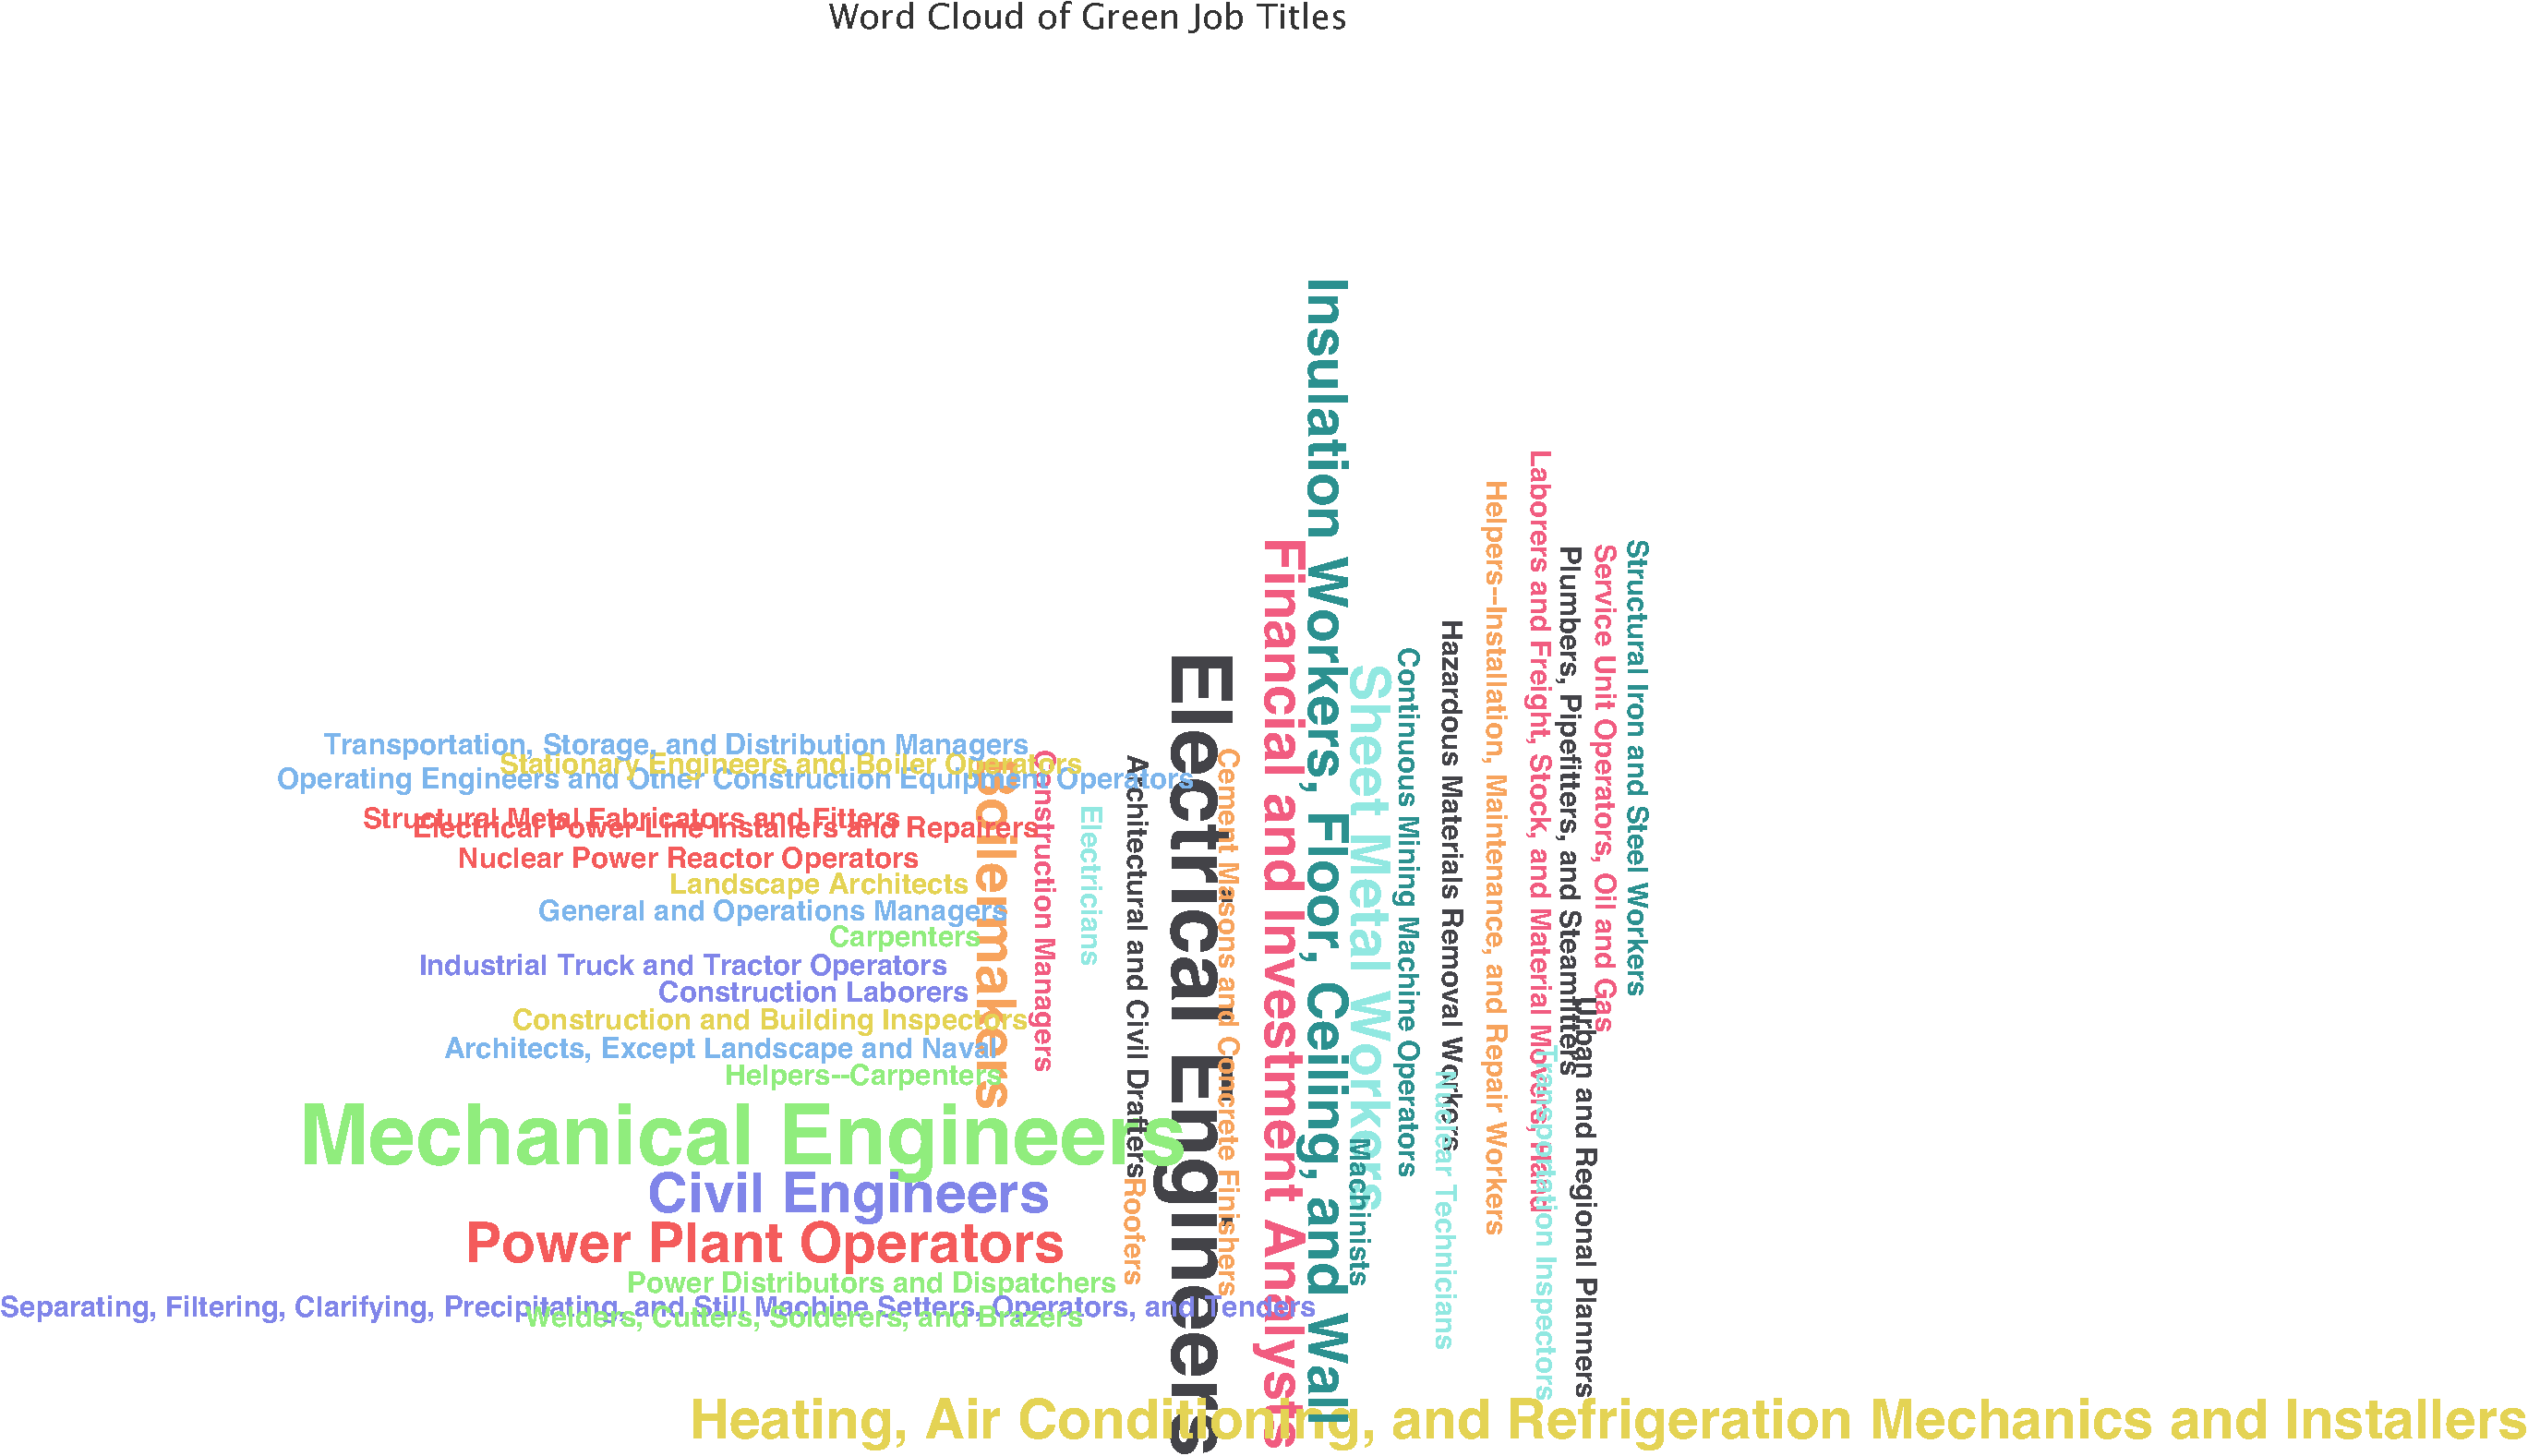
\includegraphics{index_files/figure-pdf/unnamed-chunk-16-1.pdf}

\textsubscript{Source:
\href{https://beeckcenter.github.io/climate-equity-workforce/index-preview.html}{Article
Notebook}}

Now let's create separate word clouds for each of the green sectors
(``Energy Efficiency'', ``Renewable Energy Generation'', and ``Green
Construction'').

\begin{Shaded}
\begin{Highlighting}[]
\CommentTok{\# Filter the dataset for each sector}
\NormalTok{energy\_efficiency\_jobs }\OtherTok{\textless{}{-}}\NormalTok{ national\_jobs }\SpecialCharTok{\%\textgreater{}\%}
  \FunctionTok{filter}\NormalTok{(}\StringTok{\textasciigrave{}}\AttributeTok{O*NET{-}SOC Sector}\StringTok{\textasciigrave{}} \SpecialCharTok{==} \StringTok{"Energy Efficiency"}\NormalTok{)}

\NormalTok{renewable\_energy\_jobs }\OtherTok{\textless{}{-}}\NormalTok{ national\_jobs }\SpecialCharTok{\%\textgreater{}\%}
  \FunctionTok{filter}\NormalTok{(}\StringTok{\textasciigrave{}}\AttributeTok{O*NET{-}SOC Sector}\StringTok{\textasciigrave{}} \SpecialCharTok{==} \StringTok{"Renewable Energy Generation"}\NormalTok{)}

\NormalTok{green\_construction\_jobs }\OtherTok{\textless{}{-}}\NormalTok{ national\_jobs }\SpecialCharTok{\%\textgreater{}\%}
  \FunctionTok{filter}\NormalTok{(}\StringTok{\textasciigrave{}}\AttributeTok{O*NET{-}SOC Sector}\StringTok{\textasciigrave{}} \SpecialCharTok{==} \StringTok{"Green Construction"}\NormalTok{)}

\CommentTok{\# Create a function to generate word clouds}
\NormalTok{generate\_wordcloud }\OtherTok{\textless{}{-}} \ControlFlowTok{function}\NormalTok{(data, sector\_name) \{}
\NormalTok{  job\_titles }\OtherTok{\textless{}{-}}\NormalTok{ data }\SpecialCharTok{\%\textgreater{}\%}
    \FunctionTok{count}\NormalTok{(OCC\_TITLE, }\AttributeTok{sort =} \ConstantTok{TRUE}\NormalTok{)}
  
  \FunctionTok{hchart}\NormalTok{(}
\NormalTok{    job\_titles, }
    \StringTok{"wordcloud"}\NormalTok{, }
    \FunctionTok{hcaes}\NormalTok{(}\AttributeTok{name =}\NormalTok{ OCC\_TITLE, }\AttributeTok{weight =}\NormalTok{ n)}
\NormalTok{  ) }\SpecialCharTok{\%\textgreater{}\%}
    \FunctionTok{hc\_title}\NormalTok{(}\AttributeTok{text =} \FunctionTok{paste}\NormalTok{(}\StringTok{"Word Cloud of"}\NormalTok{, sector\_name, }\StringTok{"Job Titles"}\NormalTok{))}
\NormalTok{\}}

\CommentTok{\# Generate word cloud for Energy Efficiency}
\NormalTok{energy\_efficiency\_wordcloud }\OtherTok{\textless{}{-}} \FunctionTok{generate\_wordcloud}\NormalTok{(energy\_efficiency\_jobs, }\StringTok{"Energy Efficiency"}\NormalTok{)}

\CommentTok{\# Generate word cloud for Renewable Energy Generation}
\NormalTok{renewable\_energy\_wordcloud }\OtherTok{\textless{}{-}} \FunctionTok{generate\_wordcloud}\NormalTok{(renewable\_energy\_jobs, }\StringTok{"Renewable Energy Generation"}\NormalTok{)}

\CommentTok{\# Generate word cloud for Green Construction}
\NormalTok{green\_construction\_wordcloud }\OtherTok{\textless{}{-}} \FunctionTok{generate\_wordcloud}\NormalTok{(green\_construction\_jobs, }\StringTok{"Green Construction"}\NormalTok{)}

\CommentTok{\# Display the word clouds}
\NormalTok{energy\_efficiency\_wordcloud}
\end{Highlighting}
\end{Shaded}

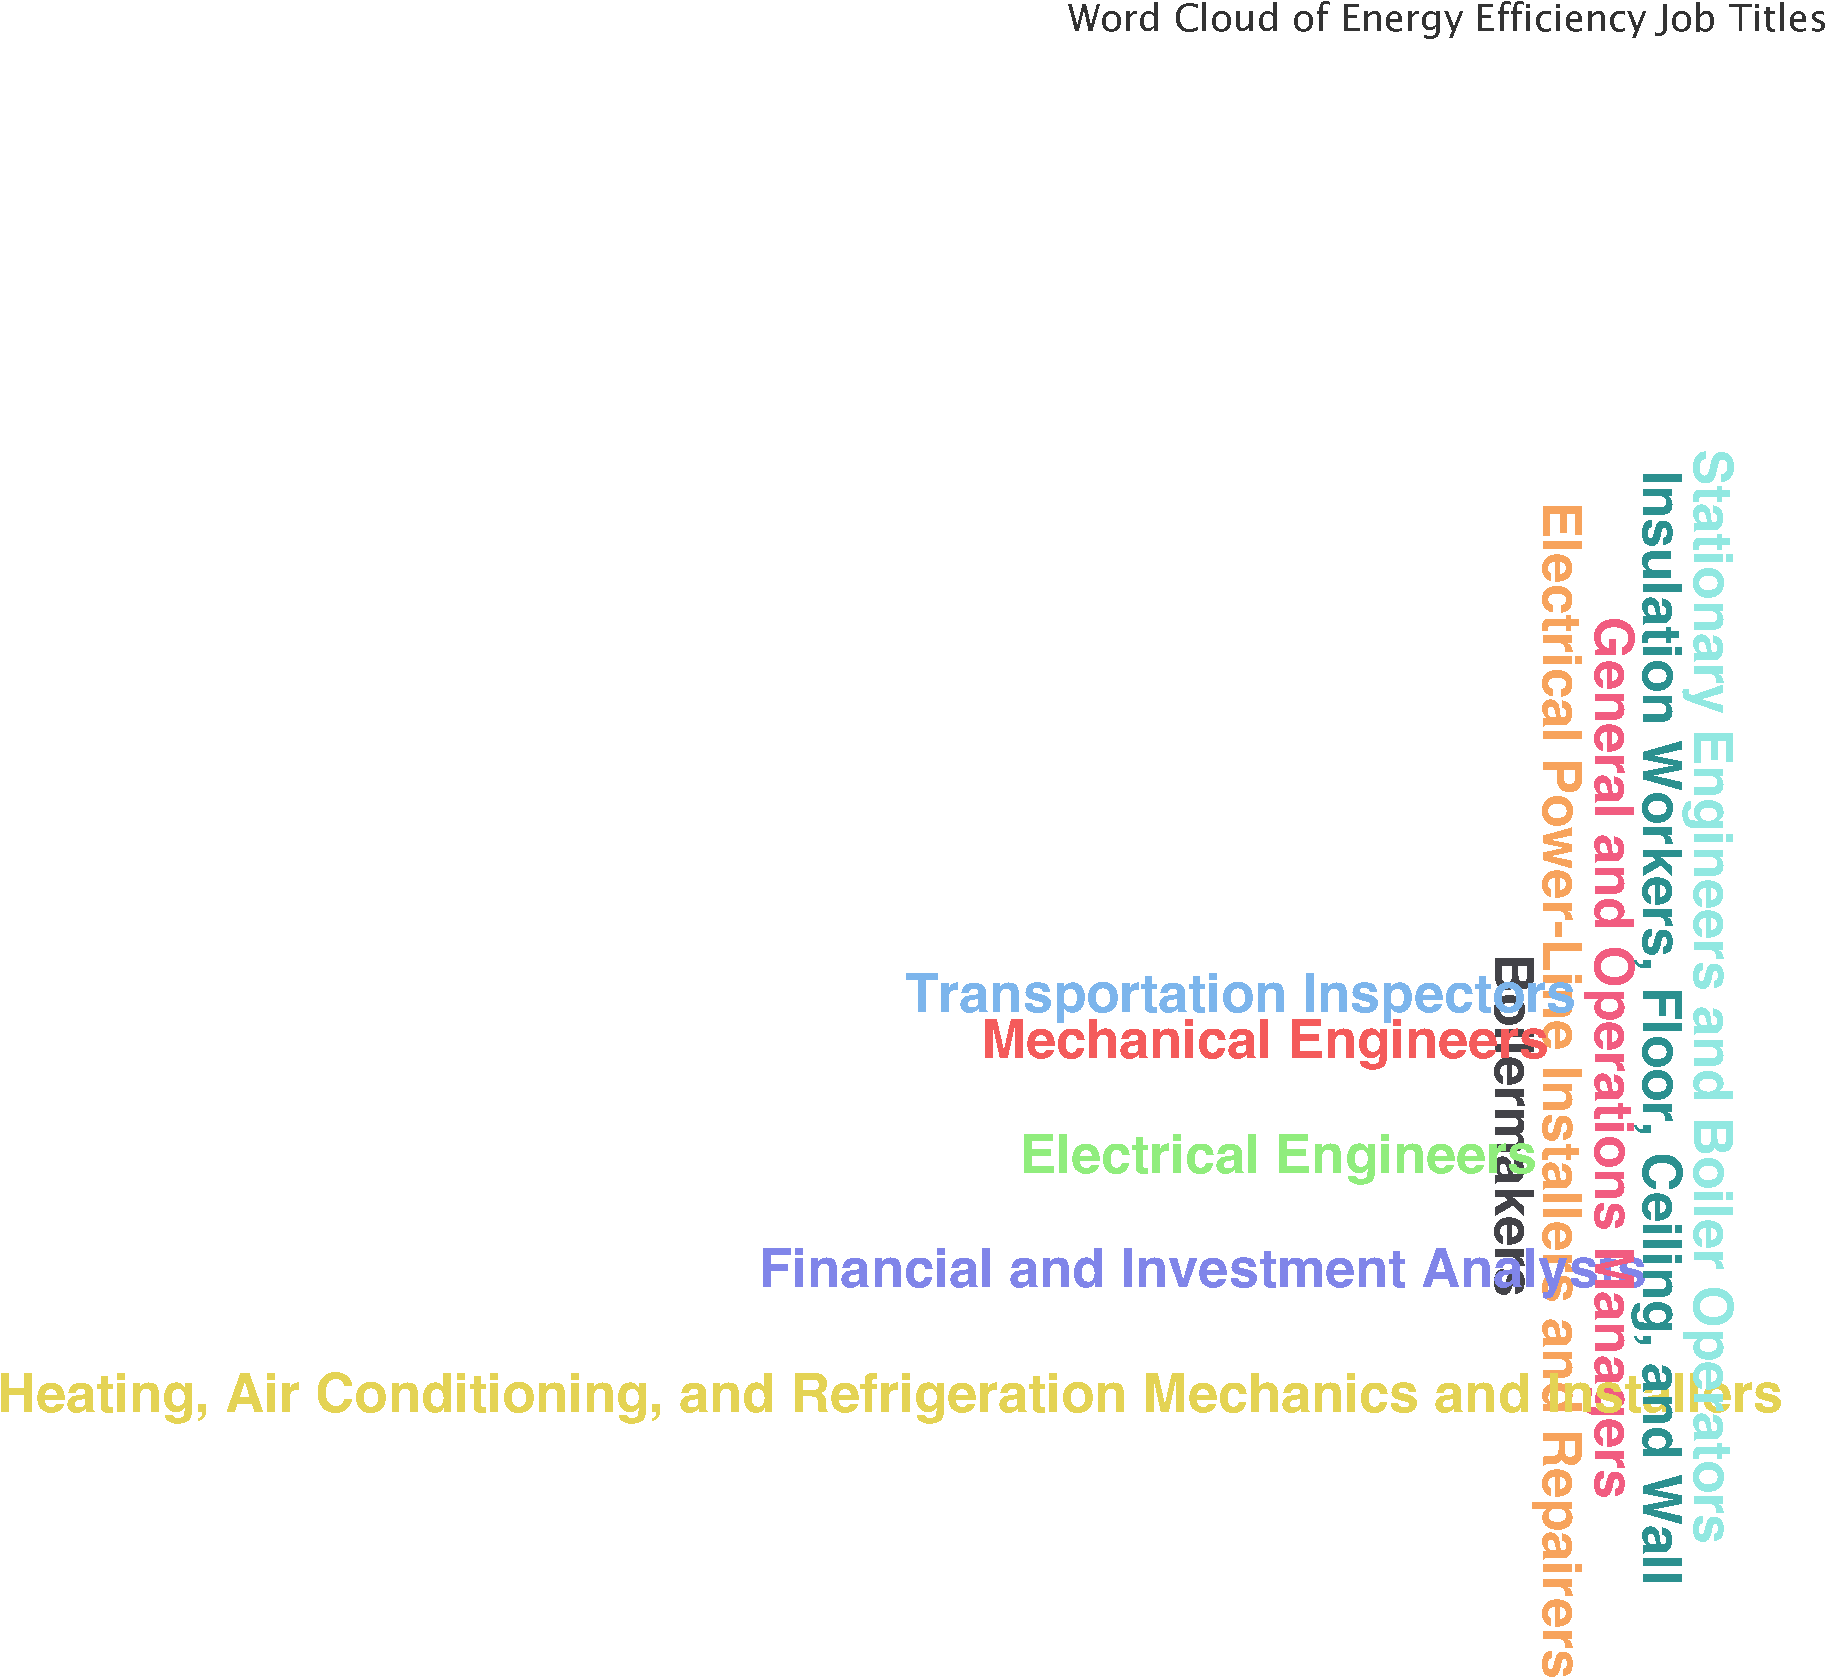
\includegraphics{index_files/figure-pdf/unnamed-chunk-17-1.pdf}

\begin{Shaded}
\begin{Highlighting}[]
\NormalTok{renewable\_energy\_wordcloud}
\end{Highlighting}
\end{Shaded}

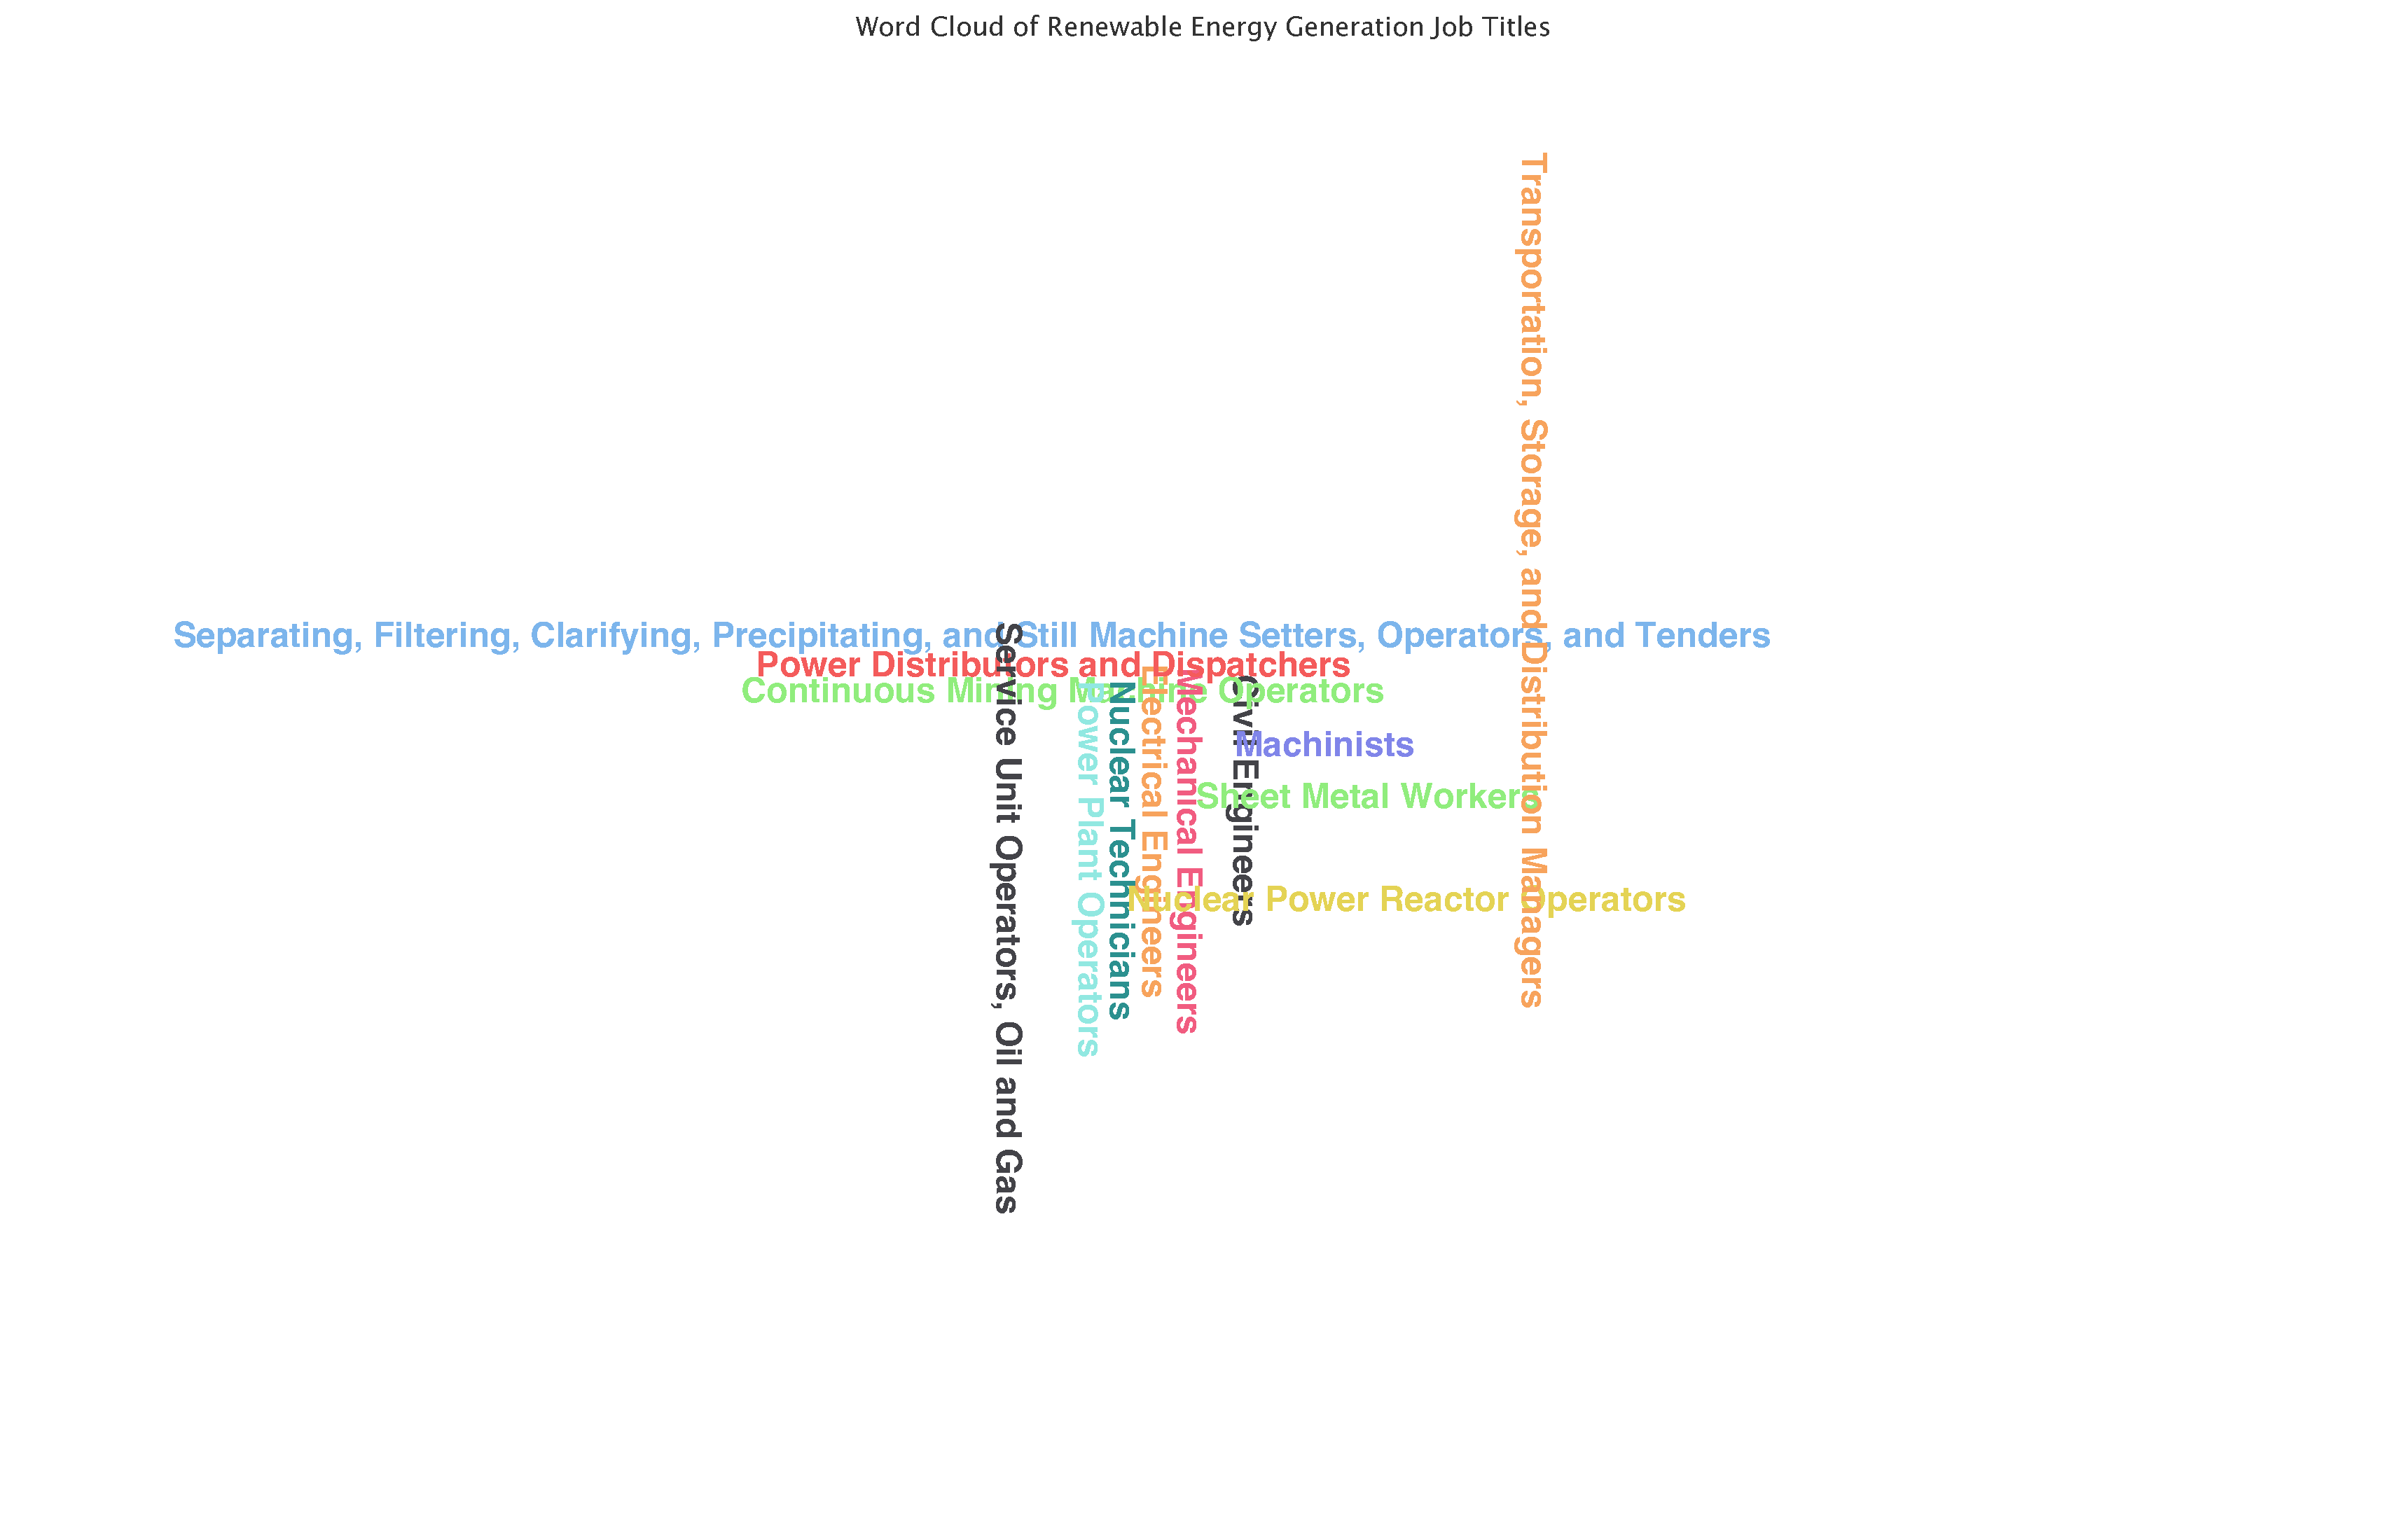
\includegraphics{index_files/figure-pdf/unnamed-chunk-17-2.pdf}

\begin{Shaded}
\begin{Highlighting}[]
\NormalTok{green\_construction\_wordcloud}
\end{Highlighting}
\end{Shaded}

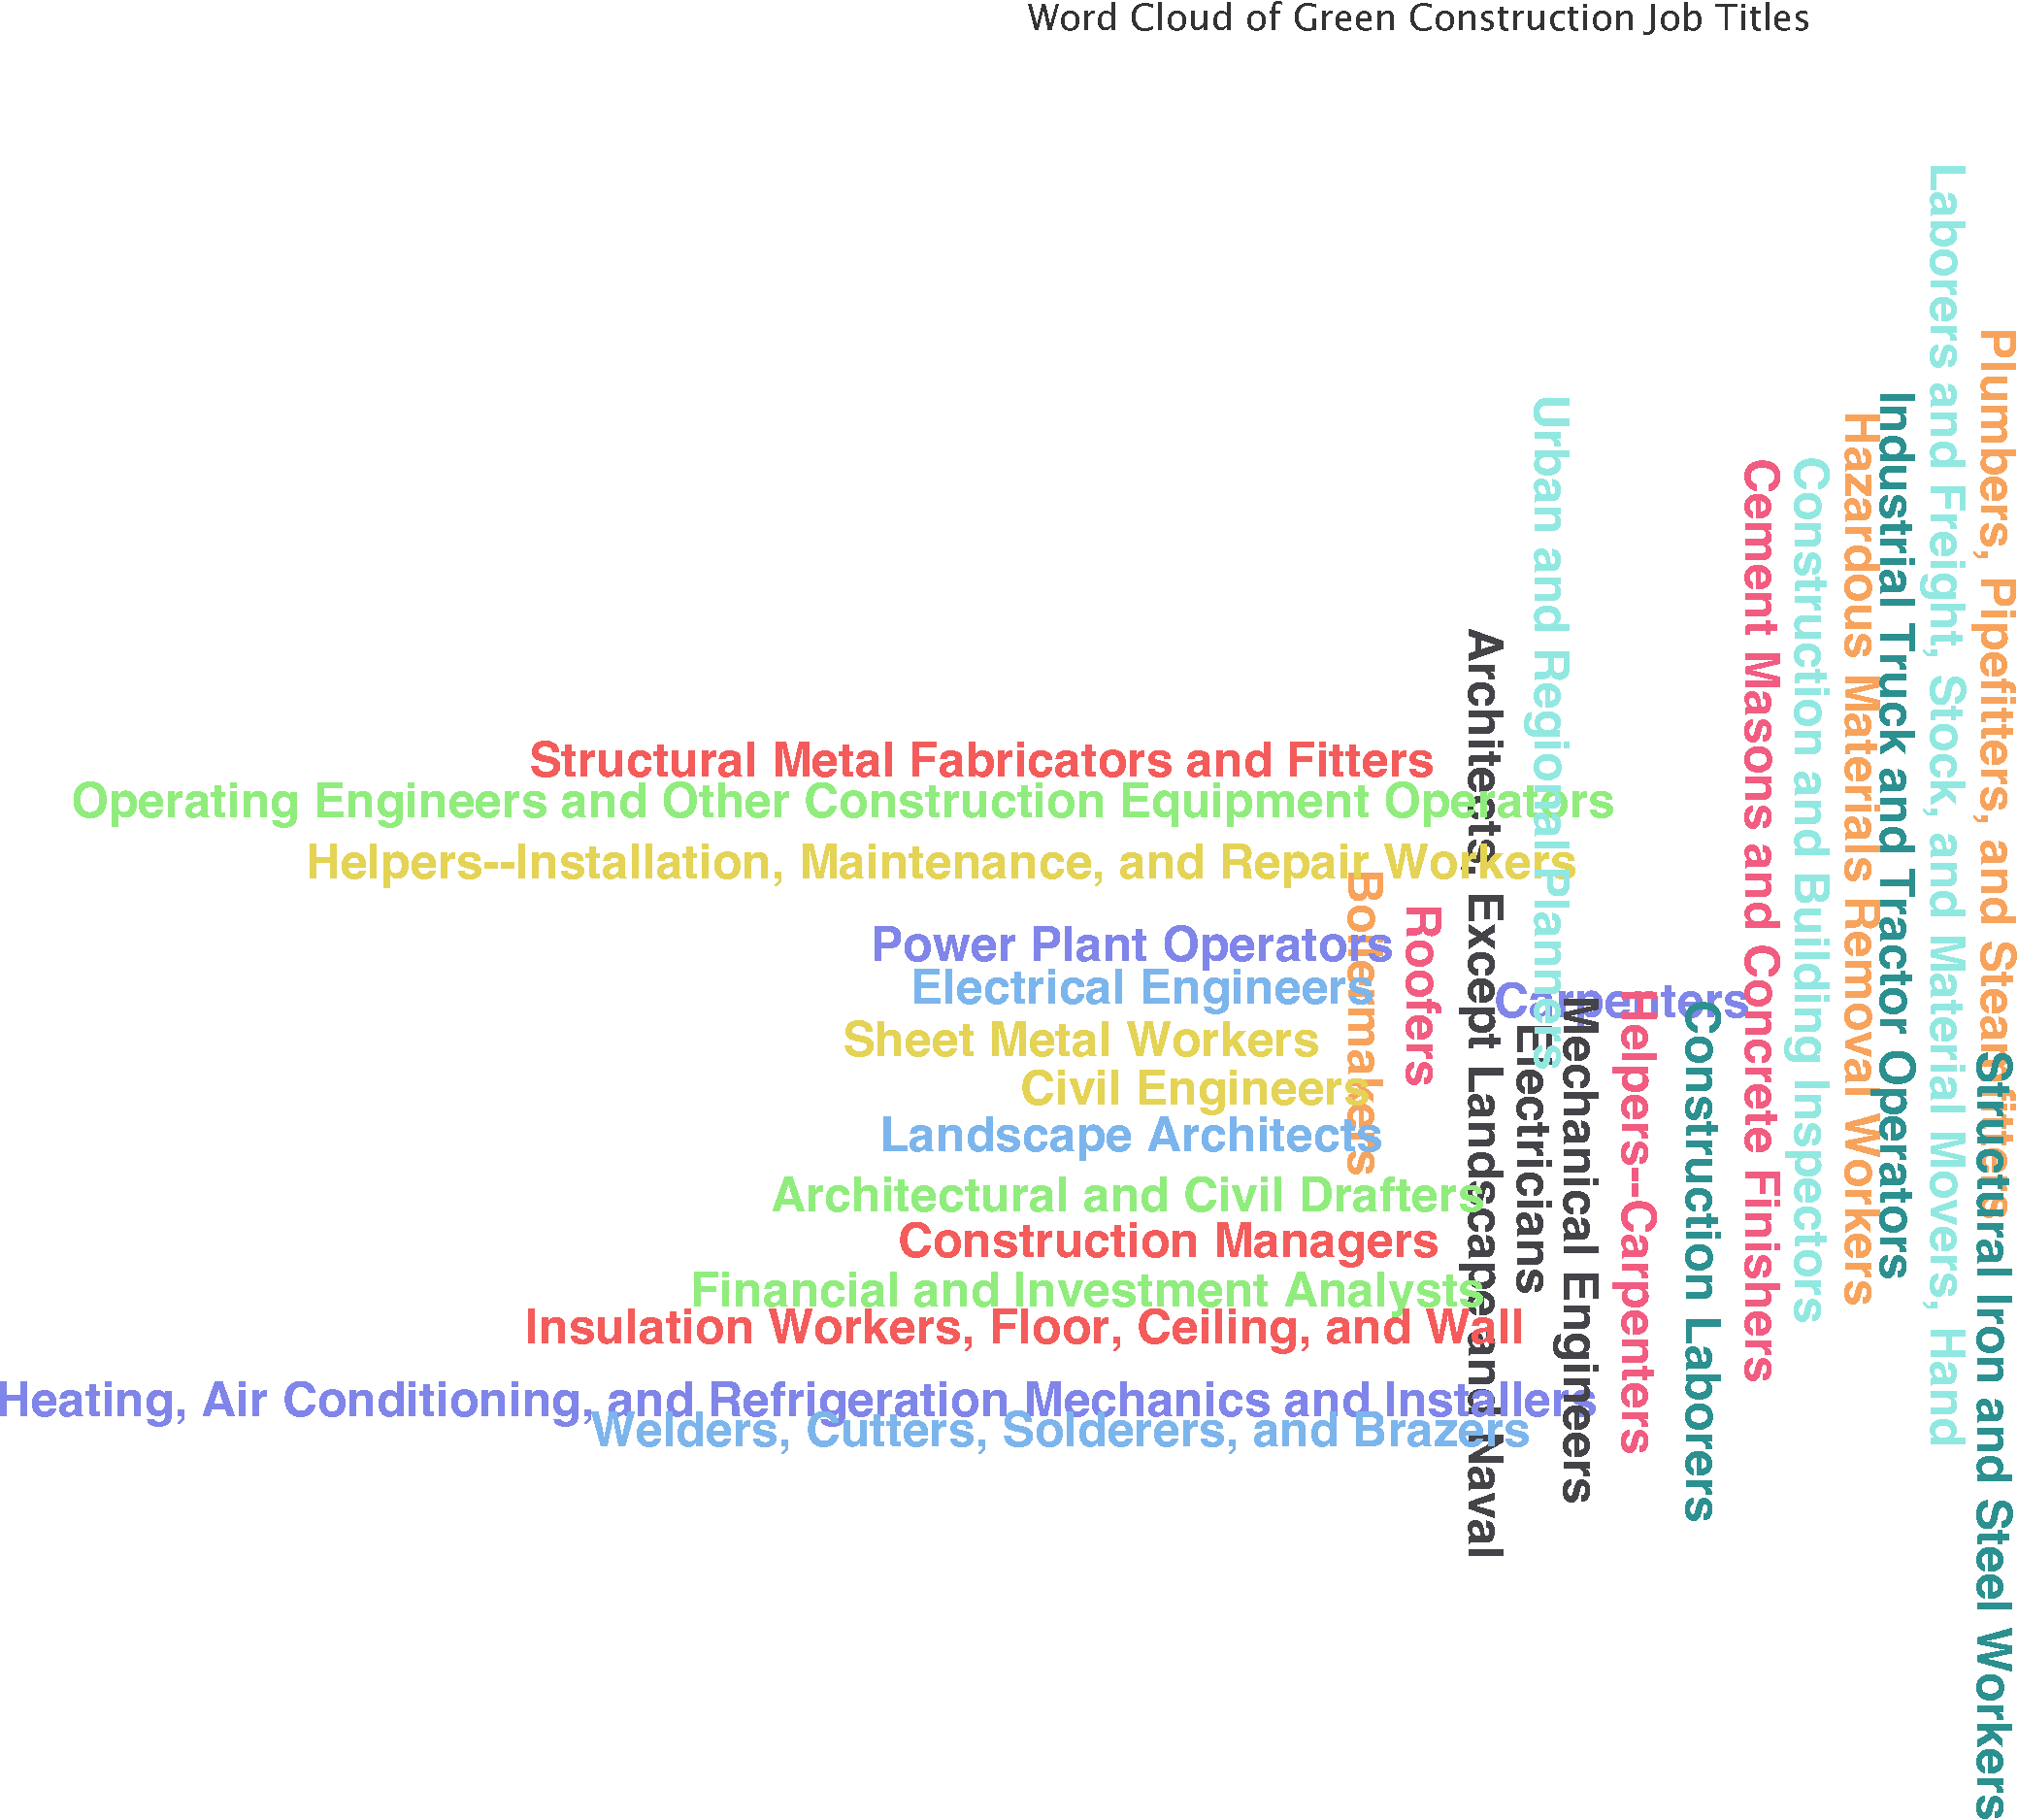
\includegraphics{index_files/figure-pdf/unnamed-chunk-17-3.pdf}

\textsubscript{Source:
\href{https://beeckcenter.github.io/climate-equity-workforce/index-preview.html}{Article
Notebook}}

Let's export for graphing

\begin{Shaded}
\begin{Highlighting}[]
\DocumentationTok{\#\# Export the national jobs data to CSV for graphing}
\FunctionTok{write.csv}\NormalTok{(national\_jobs, }\FunctionTok{here}\NormalTok{(}\StringTok{"processed\_data"}\NormalTok{, }\StringTok{"national\_jobs.csv"}\NormalTok{), }\AttributeTok{row.names =} \ConstantTok{FALSE}\NormalTok{)}

\CommentTok{\# Export the job\_type\_summary dataset to CSV for graphing}
\FunctionTok{write.csv}\NormalTok{(job\_type\_summary, }\FunctionTok{here}\NormalTok{(}\StringTok{"processed\_data"}\NormalTok{, }\StringTok{"national\_job\_type\_summary.csv"}\NormalTok{), }\AttributeTok{row.names =} \ConstantTok{FALSE}\NormalTok{)}
\end{Highlighting}
\end{Shaded}

\textsubscript{Source:
\href{https://beeckcenter.github.io/climate-equity-workforce/index-preview.html}{Article
Notebook}}

\paragraph{Green jobs in St.~Paul}\label{green-jobs-in-st.-paul}

\begin{Shaded}
\begin{Highlighting}[]
\CommentTok{\# Import St. Paul jobs data}
\NormalTok{st\_paul\_jobs }\OtherTok{\textless{}{-}} \FunctionTok{read\_csv}\NormalTok{(}\FunctionTok{here}\NormalTok{(}\StringTok{"processed\_data"}\NormalTok{, }\StringTok{"OWES\_and\_ONET{-}St\_Paul.csv"}\NormalTok{))}
\end{Highlighting}
\end{Shaded}

\begin{verbatim}
Rows: 742 Columns: 34
-- Column specification --------------------------------------------------------
Delimiter: ","
chr (26): AREA_TITLE, PRIM_STATE, NAICS_TITLE, I_GROUP, OCC_CODE, OCC_TITLE,...
dbl  (4): AREA, AREA_TYPE, NAICS, OWN_CODE
lgl  (4): PCT_TOTAL, PCT_RPT, ANNUAL, HOURLY

i Use `spec()` to retrieve the full column specification for this data.
i Specify the column types or set `show_col_types = FALSE` to quiet this message.
\end{verbatim}

\begin{Shaded}
\begin{Highlighting}[]
\FunctionTok{saveRDS}\NormalTok{(st\_paul\_jobs, }\FunctionTok{here}\NormalTok{(}\StringTok{"processed\_data"}\NormalTok{, }\StringTok{"st\_paul\_jobs.rds"}\NormalTok{))}

\NormalTok{st\_paul\_jobs }\OtherTok{\textless{}{-}} \FunctionTok{readRDS}\NormalTok{(}\FunctionTok{here}\NormalTok{(}\StringTok{"processed\_data"}\NormalTok{, }\StringTok{"st\_paul\_jobs.rds"}\NormalTok{))}
\end{Highlighting}
\end{Shaded}

\textsubscript{Source:
\href{https://beeckcenter.github.io/climate-equity-workforce/index-preview.html}{Article
Notebook}}

\begin{Shaded}
\begin{Highlighting}[]
\CommentTok{\# Convert necessary columns to numeric where needed}
\NormalTok{st\_paul\_jobs }\OtherTok{\textless{}{-}}\NormalTok{ st\_paul\_jobs }\SpecialCharTok{\%\textgreater{}\%}
  \FunctionTok{mutate}\NormalTok{(}
    \AttributeTok{TOT\_EMP =} \FunctionTok{as.numeric}\NormalTok{(TOT\_EMP),}
    \AttributeTok{H\_MEAN =} \FunctionTok{as.numeric}\NormalTok{(H\_MEAN),}
    \AttributeTok{A\_MEAN =} \FunctionTok{as.numeric}\NormalTok{(A\_MEAN),}
    \AttributeTok{A\_MEDIAN =} \FunctionTok{as.numeric}\NormalTok{(A\_MEDIAN),}
    \AttributeTok{H\_MEDIAN =} \FunctionTok{as.numeric}\NormalTok{(H\_MEDIAN)}
\NormalTok{  )}
\end{Highlighting}
\end{Shaded}

\begin{verbatim}
Warning: There were 5 warnings in `mutate()`.
The first warning was:
i In argument: `TOT_EMP = as.numeric(TOT_EMP)`.
Caused by warning:
! NAs introduced by coercion
i Run `dplyr::last_dplyr_warnings()` to see the 4 remaining warnings.
\end{verbatim}

\begin{Shaded}
\begin{Highlighting}[]
\CommentTok{\# Filter the dataset to include only relevant green sectors}
\NormalTok{filtered\_st\_paul\_jobs }\OtherTok{\textless{}{-}}\NormalTok{ st\_paul\_jobs }\SpecialCharTok{\%\textgreater{}\%}
  \FunctionTok{filter}\NormalTok{(}\StringTok{\textasciigrave{}}\AttributeTok{O*NET{-}SOC Sector}\StringTok{\textasciigrave{}} \SpecialCharTok{\%in\%} \FunctionTok{c}\NormalTok{(}\StringTok{"Energy Efficiency"}\NormalTok{, }\StringTok{"Renewable Energy Generation"}\NormalTok{, }\StringTok{"Green Construction"}\NormalTok{))}

\CommentTok{\# Function to summarize data for each sector}
\NormalTok{summarize\_by\_sector }\OtherTok{\textless{}{-}} \ControlFlowTok{function}\NormalTok{(df) \{}
\NormalTok{  df }\SpecialCharTok{\%\textgreater{}\%}
    \FunctionTok{summarize}\NormalTok{(}
      \AttributeTok{TOT\_EMP =} \FunctionTok{sum}\NormalTok{(TOT\_EMP, }\AttributeTok{na.rm =} \ConstantTok{TRUE}\NormalTok{),}
      \AttributeTok{H\_MEAN =} \FunctionTok{mean}\NormalTok{(H\_MEAN, }\AttributeTok{na.rm =} \ConstantTok{TRUE}\NormalTok{),}
      \AttributeTok{A\_MEAN =} \FunctionTok{mean}\NormalTok{(A\_MEAN, }\AttributeTok{na.rm =} \ConstantTok{TRUE}\NormalTok{),}
      \AttributeTok{A\_MEDIAN =} \FunctionTok{median}\NormalTok{(A\_MEDIAN, }\AttributeTok{na.rm =} \ConstantTok{TRUE}\NormalTok{),}
      \AttributeTok{H\_MEDIAN =} \FunctionTok{median}\NormalTok{(H\_MEDIAN, }\AttributeTok{na.rm =} \ConstantTok{TRUE}\NormalTok{)}
\NormalTok{    )}
\NormalTok{\}}

\CommentTok{\# Summarize the data for each sector and overall}
\NormalTok{sector\_summary\_st\_paul }\OtherTok{\textless{}{-}}\NormalTok{ filtered\_st\_paul\_jobs }\SpecialCharTok{\%\textgreater{}\%}
  \FunctionTok{group\_by}\NormalTok{(}\StringTok{\textasciigrave{}}\AttributeTok{O*NET{-}SOC Sector}\StringTok{\textasciigrave{}}\NormalTok{) }\SpecialCharTok{\%\textgreater{}\%}
  \FunctionTok{summarize\_by\_sector}\NormalTok{()}

\CommentTok{\# Calculate the summary for all sectors combined}
\NormalTok{overall\_summary\_st\_paul }\OtherTok{\textless{}{-}}\NormalTok{ filtered\_st\_paul\_jobs }\SpecialCharTok{\%\textgreater{}\%}
  \FunctionTok{summarize\_by\_sector}\NormalTok{()}

\CommentTok{\# Combine the results: sector{-}wise and overall}
\NormalTok{final\_summary\_st\_paul }\OtherTok{\textless{}{-}} \FunctionTok{bind\_rows}\NormalTok{(sector\_summary\_st\_paul, }\FunctionTok{tibble}\NormalTok{(}\StringTok{\textasciigrave{}}\AttributeTok{O*NET{-}SOC Sector}\StringTok{\textasciigrave{}} \OtherTok{=} \StringTok{"All"}\NormalTok{, overall\_summary\_st\_paul))}

\CommentTok{\# Save the final summary as an RDS file and CSV for future reference}
\FunctionTok{saveRDS}\NormalTok{(final\_summary\_st\_paul, }\FunctionTok{here}\NormalTok{(}\StringTok{"processed\_data"}\NormalTok{, }\StringTok{"sector\_summary\_st\_paul.rds"}\NormalTok{))}
\FunctionTok{write\_csv}\NormalTok{(final\_summary\_st\_paul, }\FunctionTok{here}\NormalTok{(}\StringTok{"processed\_data"}\NormalTok{, }\StringTok{"sector\_summary\_st\_paul.csv"}\NormalTok{))}

\CommentTok{\# Output the final summary to the user}
\FunctionTok{print}\NormalTok{(final\_summary\_st\_paul)}
\end{Highlighting}
\end{Shaded}

\begin{verbatim}
# A tibble: 4 x 6
  `O*NET-SOC Sector`          TOT_EMP H_MEAN A_MEAN A_MEDIAN H_MEDIAN
  <chr>                         <dbl>  <dbl>  <dbl>    <dbl>    <dbl>
1 Energy Efficiency             66410   45.5 94669.    98740     47.5
2 Green Construction           124680   37.9 78809.    75800     36.4
3 Renewable Energy Generation   23250   44.7 92991.    99690     47.9
4 All                          214340   40.7 84562.    82170     39.5
\end{verbatim}

\begin{Shaded}
\begin{Highlighting}[]
\CommentTok{\# Calculate total employment and sector percentages for St. Paul}
\NormalTok{total\_green\_jobs\_st\_paul }\OtherTok{\textless{}{-}}\NormalTok{ final\_summary\_st\_paul }\SpecialCharTok{\%\textgreater{}\%} \FunctionTok{filter}\NormalTok{(}\StringTok{\textasciigrave{}}\AttributeTok{O*NET{-}SOC Sector}\StringTok{\textasciigrave{}} \SpecialCharTok{==} \StringTok{"All"}\NormalTok{) }\SpecialCharTok{\%\textgreater{}\%} \FunctionTok{pull}\NormalTok{(TOT\_EMP)}

\NormalTok{energy\_efficiency\_jobs\_st\_paul }\OtherTok{\textless{}{-}}\NormalTok{ final\_summary\_st\_paul }\SpecialCharTok{\%\textgreater{}\%} \FunctionTok{filter}\NormalTok{(}\StringTok{\textasciigrave{}}\AttributeTok{O*NET{-}SOC Sector}\StringTok{\textasciigrave{}} \SpecialCharTok{==} \StringTok{"Energy Efficiency"}\NormalTok{) }\SpecialCharTok{\%\textgreater{}\%} \FunctionTok{pull}\NormalTok{(TOT\_EMP)}
\NormalTok{green\_construction\_jobs\_st\_paul }\OtherTok{\textless{}{-}}\NormalTok{ final\_summary\_st\_paul }\SpecialCharTok{\%\textgreater{}\%} \FunctionTok{filter}\NormalTok{(}\StringTok{\textasciigrave{}}\AttributeTok{O*NET{-}SOC Sector}\StringTok{\textasciigrave{}} \SpecialCharTok{==} \StringTok{"Green Construction"}\NormalTok{) }\SpecialCharTok{\%\textgreater{}\%} \FunctionTok{pull}\NormalTok{(TOT\_EMP)}
\NormalTok{renewable\_energy\_jobs\_st\_paul }\OtherTok{\textless{}{-}}\NormalTok{ final\_summary\_st\_paul }\SpecialCharTok{\%\textgreater{}\%} \FunctionTok{filter}\NormalTok{(}\StringTok{\textasciigrave{}}\AttributeTok{O*NET{-}SOC Sector}\StringTok{\textasciigrave{}} \SpecialCharTok{==} \StringTok{"Renewable Energy Generation"}\NormalTok{) }\SpecialCharTok{\%\textgreater{}\%} \FunctionTok{pull}\NormalTok{(TOT\_EMP)}

\CommentTok{\# Calculate the percentages}
\NormalTok{energy\_efficiency\_pct\_st\_paul }\OtherTok{\textless{}{-}} \FunctionTok{round}\NormalTok{((energy\_efficiency\_jobs\_st\_paul }\SpecialCharTok{/}\NormalTok{ total\_green\_jobs\_st\_paul) }\SpecialCharTok{*} \DecValTok{100}\NormalTok{, }\DecValTok{2}\NormalTok{)}
\NormalTok{green\_construction\_pct\_st\_paul }\OtherTok{\textless{}{-}} \FunctionTok{round}\NormalTok{((green\_construction\_jobs\_st\_paul }\SpecialCharTok{/}\NormalTok{ total\_green\_jobs\_st\_paul) }\SpecialCharTok{*} \DecValTok{100}\NormalTok{, }\DecValTok{2}\NormalTok{)}
\NormalTok{renewable\_energy\_pct\_st\_paul }\OtherTok{\textless{}{-}} \FunctionTok{round}\NormalTok{((renewable\_energy\_jobs\_st\_paul }\SpecialCharTok{/}\NormalTok{ total\_green\_jobs\_st\_paul) }\SpecialCharTok{*} \DecValTok{100}\NormalTok{, }\DecValTok{2}\NormalTok{)}

\CommentTok{\# Create the concatenated sentence for St. Paul}
\FunctionTok{cat}\NormalTok{(}\StringTok{"There\textquotesingle{}s a total of"}\NormalTok{, }\FunctionTok{format}\NormalTok{(total\_green\_jobs\_st\_paul, }\AttributeTok{big.mark =} \StringTok{","}\NormalTok{, }\AttributeTok{scientific =} \ConstantTok{FALSE}\NormalTok{), }
    \StringTok{"employed people in green jobs in Saint Paul. Specifically, in Energy Efficiency, there are"}\NormalTok{, }
    \FunctionTok{format}\NormalTok{(energy\_efficiency\_jobs\_st\_paul, }\AttributeTok{big.mark =} \StringTok{","}\NormalTok{, }\AttributeTok{scientific =} \ConstantTok{FALSE}\NormalTok{), }
    \StringTok{"("}\NormalTok{, energy\_efficiency\_pct\_st\_paul, }\StringTok{"\%), in Green Construction there are"}\NormalTok{, }
    \FunctionTok{format}\NormalTok{(green\_construction\_jobs\_st\_paul, }\AttributeTok{big.mark =} \StringTok{","}\NormalTok{, }\AttributeTok{scientific =} \ConstantTok{FALSE}\NormalTok{), }
    \StringTok{"("}\NormalTok{, green\_construction\_pct\_st\_paul, }\StringTok{"\%), and in Renewable Energy Generation there are"}\NormalTok{, }
    \FunctionTok{format}\NormalTok{(renewable\_energy\_jobs\_st\_paul, }\AttributeTok{big.mark =} \StringTok{","}\NormalTok{, }\AttributeTok{scientific =} \ConstantTok{FALSE}\NormalTok{), }
    \StringTok{"("}\NormalTok{, renewable\_energy\_pct\_st\_paul, }\StringTok{"\%).}\SpecialCharTok{\textbackslash{}n}\StringTok{"}\NormalTok{)}
\end{Highlighting}
\end{Shaded}

\begin{verbatim}
There's a total of 214,340 employed people in green jobs in Saint Paul. Specifically, in Energy Efficiency, there are 66,410 ( 30.98 %), in Green Construction there are 124,680 ( 58.17 %), and in Renewable Energy Generation there are 23,250 ( 10.85 %).
\end{verbatim}

\begin{Shaded}
\begin{Highlighting}[]
\CommentTok{\# Visualizing TOT\_EMP across the green sectors for St. Paul}
\NormalTok{final\_summary\_st\_paul }\OtherTok{\textless{}{-}}\NormalTok{ final\_summary\_st\_paul }\SpecialCharTok{\%\textgreater{}\%}
  \FunctionTok{mutate}\NormalTok{(}\StringTok{\textasciigrave{}}\AttributeTok{O*NET{-}SOC Sector}\StringTok{\textasciigrave{}} \OtherTok{=} \FunctionTok{factor}\NormalTok{(}\StringTok{\textasciigrave{}}\AttributeTok{O*NET{-}SOC Sector}\StringTok{\textasciigrave{}}\NormalTok{, }\AttributeTok{levels =} \FunctionTok{c}\NormalTok{(}\StringTok{"Energy Efficiency"}\NormalTok{, }\StringTok{"Green Construction"}\NormalTok{, }\StringTok{"Renewable Energy Generation"}\NormalTok{, }\StringTok{"All"}\NormalTok{)))}

\FunctionTok{hchart}\NormalTok{(final\_summary\_st\_paul, }\StringTok{"column"}\NormalTok{, }\FunctionTok{hcaes}\NormalTok{(}\AttributeTok{x =} \StringTok{\textasciigrave{}}\AttributeTok{O*NET{-}SOC Sector}\StringTok{\textasciigrave{}}\NormalTok{, }\AttributeTok{y =}\NormalTok{ TOT\_EMP)) }\SpecialCharTok{\%\textgreater{}\%}
  \FunctionTok{hc\_title}\NormalTok{(}\AttributeTok{text =} \StringTok{"Total Employment by Sector in Saint Paul"}\NormalTok{) }\SpecialCharTok{\%\textgreater{}\%}
  \FunctionTok{hc\_xAxis}\NormalTok{(}\AttributeTok{title =} \FunctionTok{list}\NormalTok{(}\AttributeTok{text =} \StringTok{"Sector"}\NormalTok{)) }\SpecialCharTok{\%\textgreater{}\%}
  \FunctionTok{hc\_yAxis}\NormalTok{(}\AttributeTok{title =} \FunctionTok{list}\NormalTok{(}\AttributeTok{text =} \StringTok{"Total Employment"}\NormalTok{), }\AttributeTok{labels =} \FunctionTok{list}\NormalTok{(}\AttributeTok{format =} \StringTok{"\{value:,0f\}"}\NormalTok{)) }\SpecialCharTok{\%\textgreater{}\%}
  \FunctionTok{hc\_tooltip}\NormalTok{(}\AttributeTok{pointFormat =} \StringTok{\textquotesingle{}\textless{}b\textgreater{}\{point.y:,0f\}\textless{}/b\textgreater{}\textquotesingle{}}\NormalTok{)}
\end{Highlighting}
\end{Shaded}

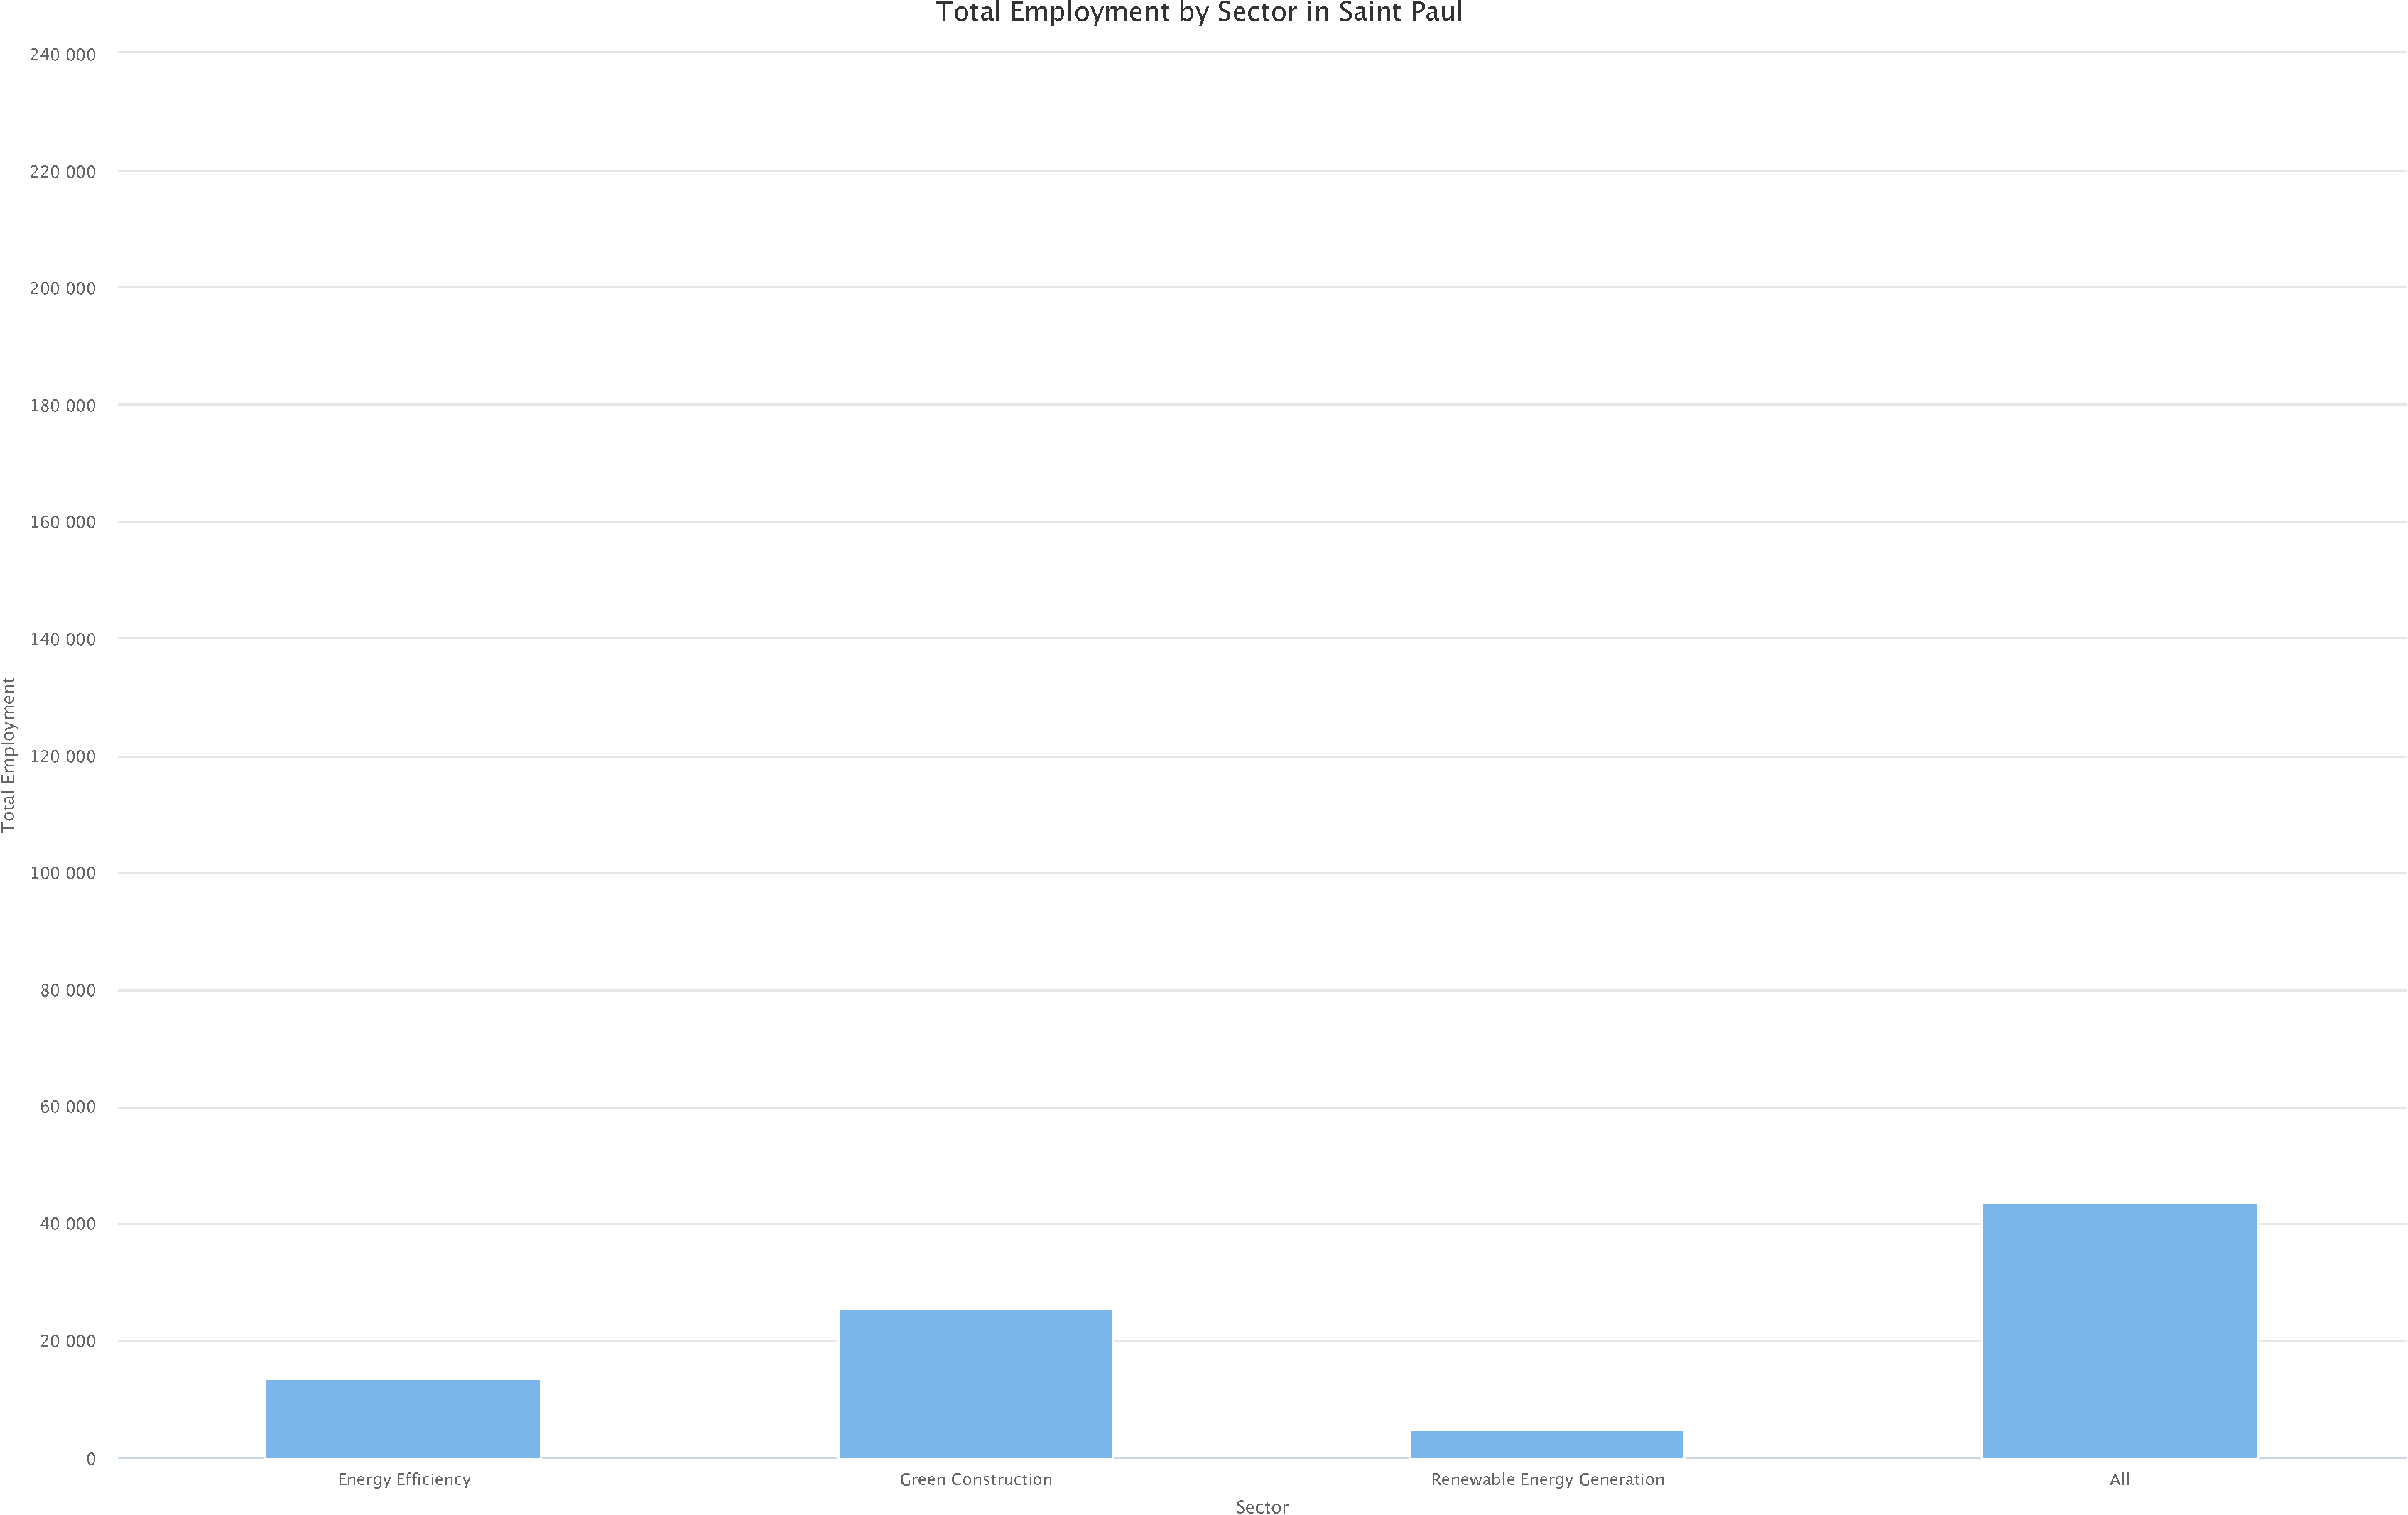
\includegraphics{index_files/figure-pdf/unnamed-chunk-20-1.pdf}

\textsubscript{Source:
\href{https://beeckcenter.github.io/climate-equity-workforce/index-preview.html}{Article
Notebook}}

\begin{Shaded}
\begin{Highlighting}[]
\CommentTok{\# Convert the O*NET{-}SOC Sector to a factor for ordering in the chart for St. Paul}
\NormalTok{final\_summary\_st\_paul }\OtherTok{\textless{}{-}}\NormalTok{ final\_summary\_st\_paul }\SpecialCharTok{\%\textgreater{}\%}
  \FunctionTok{mutate}\NormalTok{(}\StringTok{\textasciigrave{}}\AttributeTok{O*NET{-}SOC Sector}\StringTok{\textasciigrave{}} \OtherTok{=} \FunctionTok{factor}\NormalTok{(}\StringTok{\textasciigrave{}}\AttributeTok{O*NET{-}SOC Sector}\StringTok{\textasciigrave{}}\NormalTok{, }\AttributeTok{levels =} \FunctionTok{c}\NormalTok{(}\StringTok{"Energy Efficiency"}\NormalTok{, }\StringTok{"Green Construction"}\NormalTok{, }\StringTok{"Renewable Energy Generation"}\NormalTok{, }\StringTok{"All"}\NormalTok{)))}

\CommentTok{\# Visualizing TOT\_EMP across the sectors for St. Paul}
\FunctionTok{hchart}\NormalTok{(final\_summary\_st\_paul, }\StringTok{"column"}\NormalTok{, }\FunctionTok{hcaes}\NormalTok{(}\AttributeTok{x =} \StringTok{\textasciigrave{}}\AttributeTok{O*NET{-}SOC Sector}\StringTok{\textasciigrave{}}\NormalTok{, }\AttributeTok{y =}\NormalTok{ TOT\_EMP)) }\SpecialCharTok{\%\textgreater{}\%}
  \FunctionTok{hc\_title}\NormalTok{(}\AttributeTok{text =} \StringTok{"Total Employment by Sector in Saint Paul"}\NormalTok{) }\SpecialCharTok{\%\textgreater{}\%}
  \FunctionTok{hc\_xAxis}\NormalTok{(}\AttributeTok{title =} \FunctionTok{list}\NormalTok{(}\AttributeTok{text =} \StringTok{"Sector"}\NormalTok{)) }\SpecialCharTok{\%\textgreater{}\%}
  \FunctionTok{hc\_yAxis}\NormalTok{(}\AttributeTok{title =} \FunctionTok{list}\NormalTok{(}\AttributeTok{text =} \StringTok{"Total Employment"}\NormalTok{), }\AttributeTok{labels =} \FunctionTok{list}\NormalTok{(}\AttributeTok{format =} \StringTok{"\{value:,0f\}"}\NormalTok{)) }\SpecialCharTok{\%\textgreater{}\%}
  \FunctionTok{hc\_tooltip}\NormalTok{(}\AttributeTok{pointFormat =} \StringTok{\textquotesingle{}\textless{}b\textgreater{}\{point.y:,0f\}\textless{}/b\textgreater{}\textquotesingle{}}\NormalTok{)}
\end{Highlighting}
\end{Shaded}

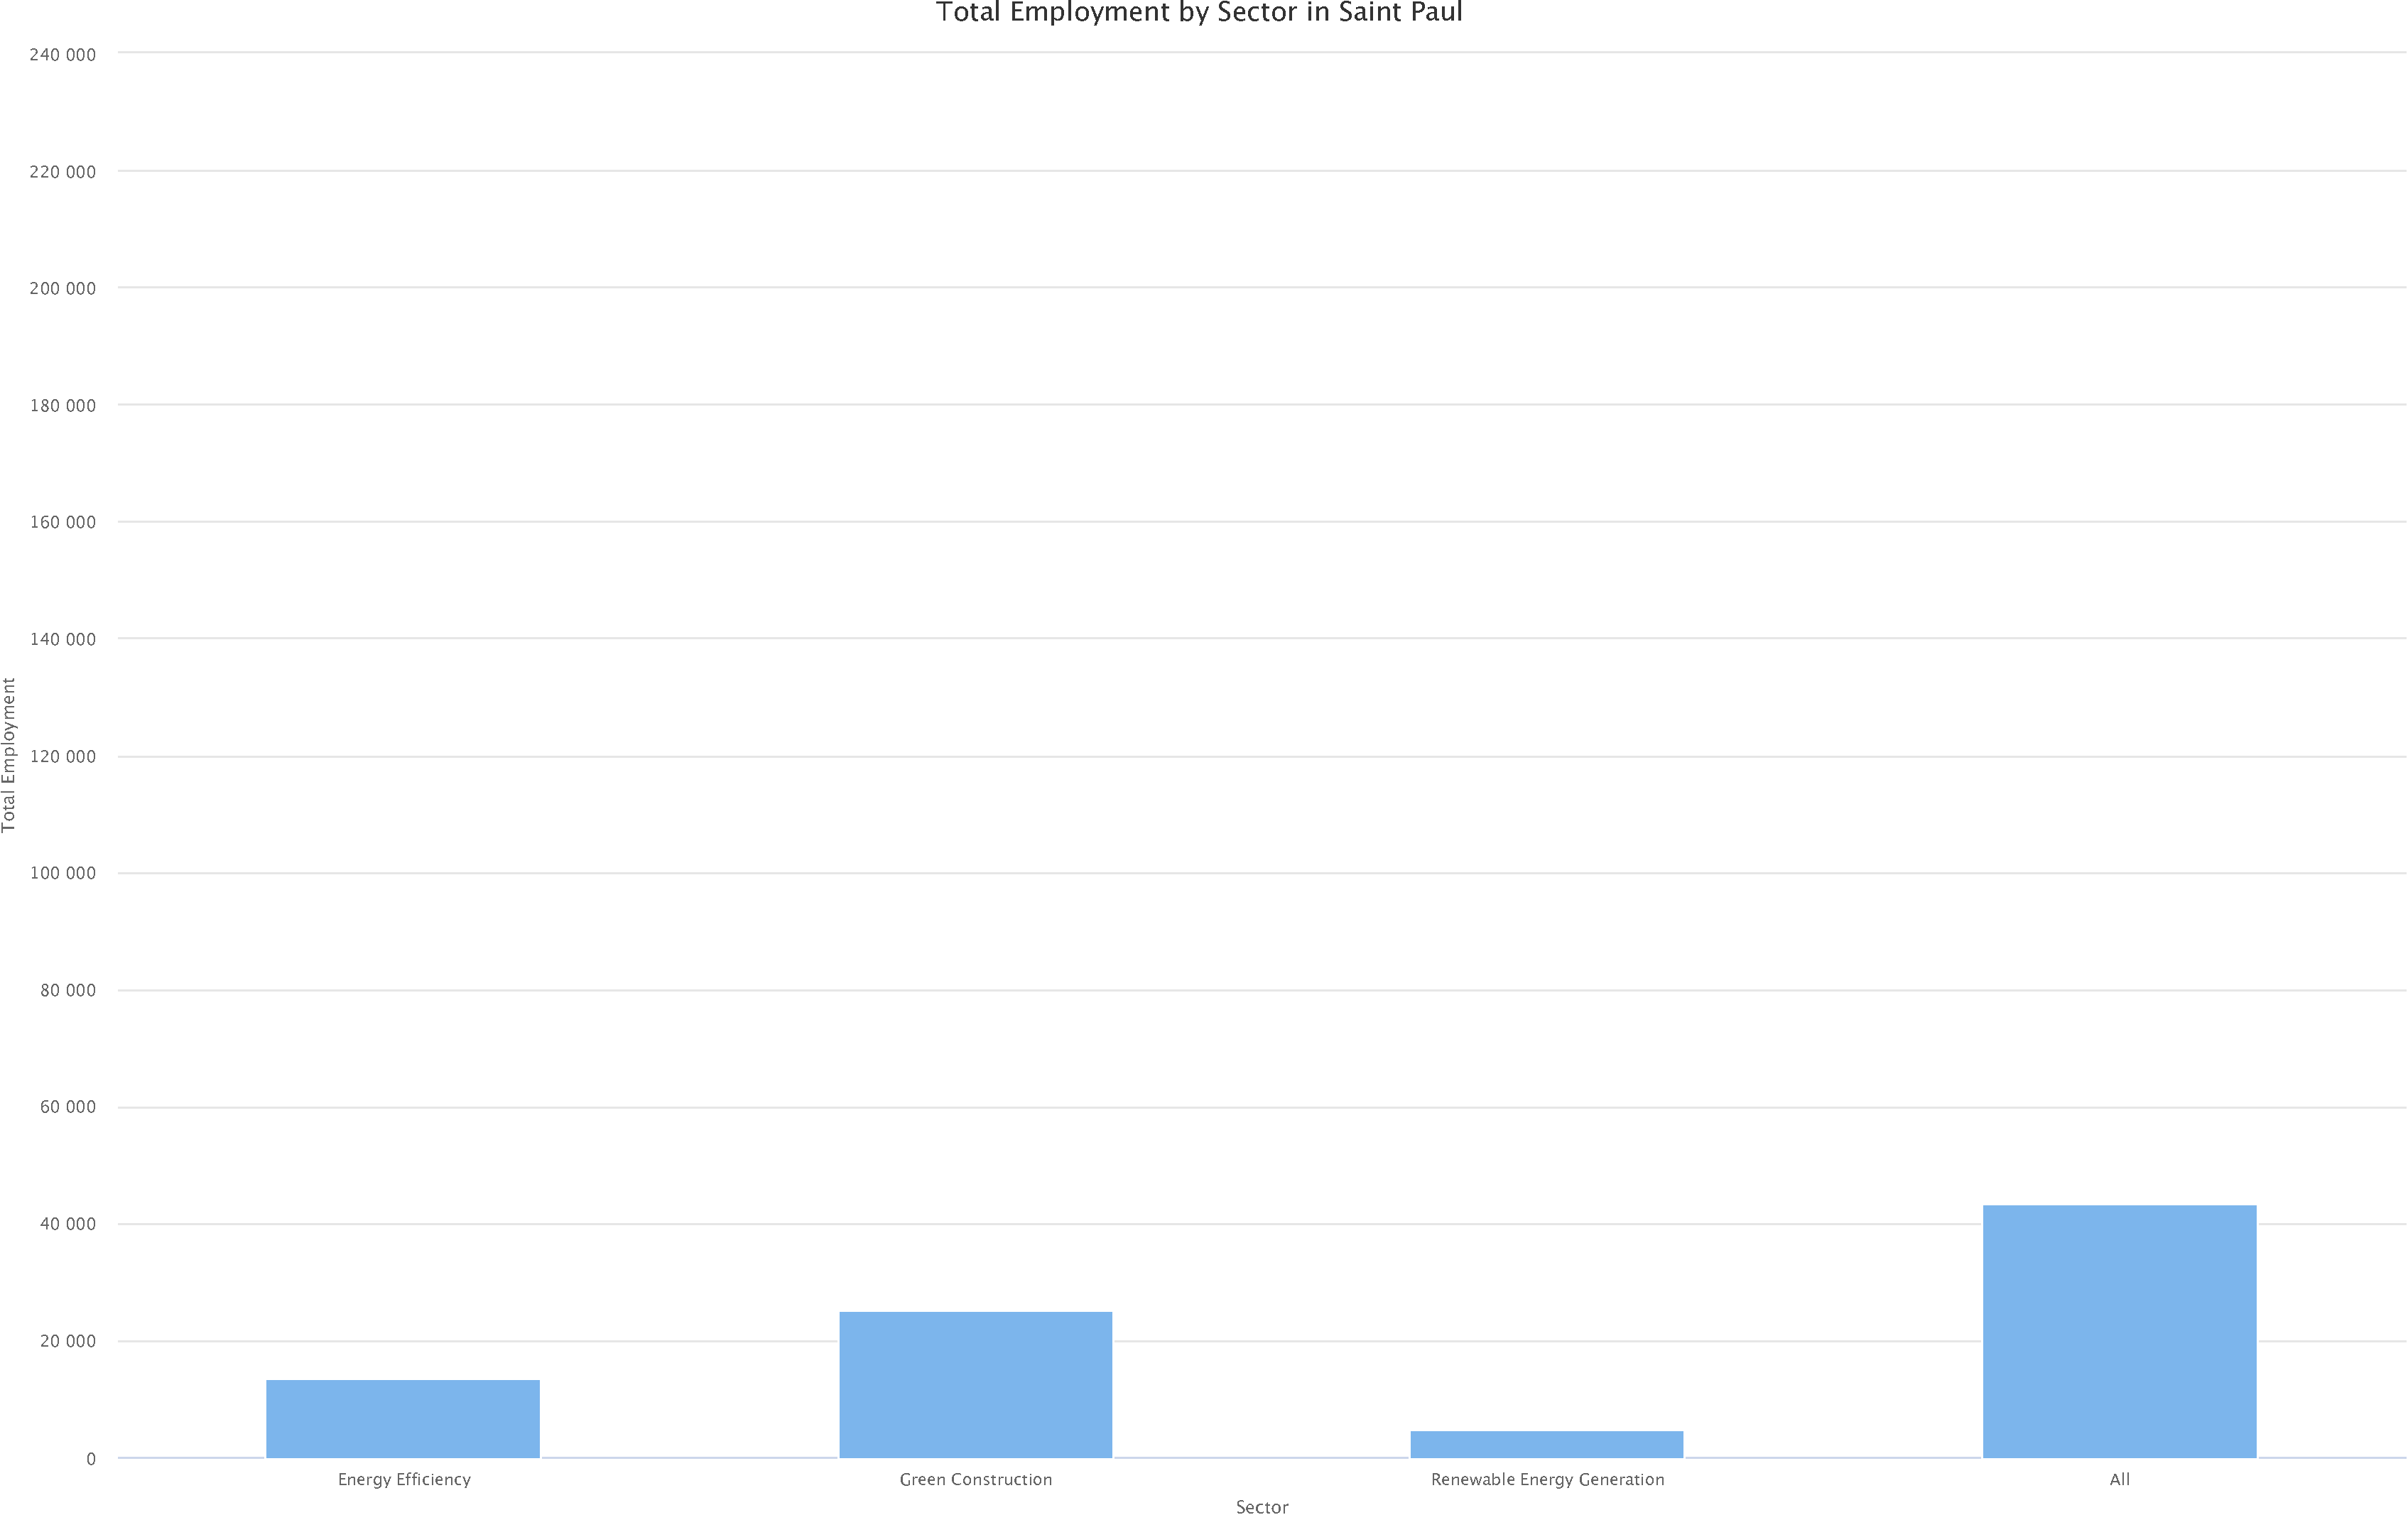
\includegraphics{index_files/figure-pdf/unnamed-chunk-21-1.pdf}

\begin{Shaded}
\begin{Highlighting}[]
\CommentTok{\# Visualizing H\_MEAN (Mean Hourly Wage) across the sectors for St. Paul}
\FunctionTok{hchart}\NormalTok{(final\_summary\_st\_paul, }\StringTok{"column"}\NormalTok{, }\FunctionTok{hcaes}\NormalTok{(}\AttributeTok{x =} \StringTok{\textasciigrave{}}\AttributeTok{O*NET{-}SOC Sector}\StringTok{\textasciigrave{}}\NormalTok{, }\AttributeTok{y =}\NormalTok{ H\_MEAN)) }\SpecialCharTok{\%\textgreater{}\%}
  \FunctionTok{hc\_title}\NormalTok{(}\AttributeTok{text =} \StringTok{"Mean Hourly Wage by Sector in Saint Paul"}\NormalTok{) }\SpecialCharTok{\%\textgreater{}\%}
  \FunctionTok{hc\_xAxis}\NormalTok{(}\AttributeTok{title =} \FunctionTok{list}\NormalTok{(}\AttributeTok{text =} \StringTok{"Sector"}\NormalTok{)) }\SpecialCharTok{\%\textgreater{}\%}
  \FunctionTok{hc\_yAxis}\NormalTok{(}\AttributeTok{title =} \FunctionTok{list}\NormalTok{(}\AttributeTok{text =} \StringTok{"Mean Hourly Wage (USD)"}\NormalTok{)) }\SpecialCharTok{\%\textgreater{}\%}
  \FunctionTok{hc\_tooltip}\NormalTok{(}\AttributeTok{pointFormat =} \StringTok{\textquotesingle{}\textless{}b\textgreater{}\{point.y:.2f\} USD\textless{}/b\textgreater{}\textquotesingle{}}\NormalTok{)}
\end{Highlighting}
\end{Shaded}

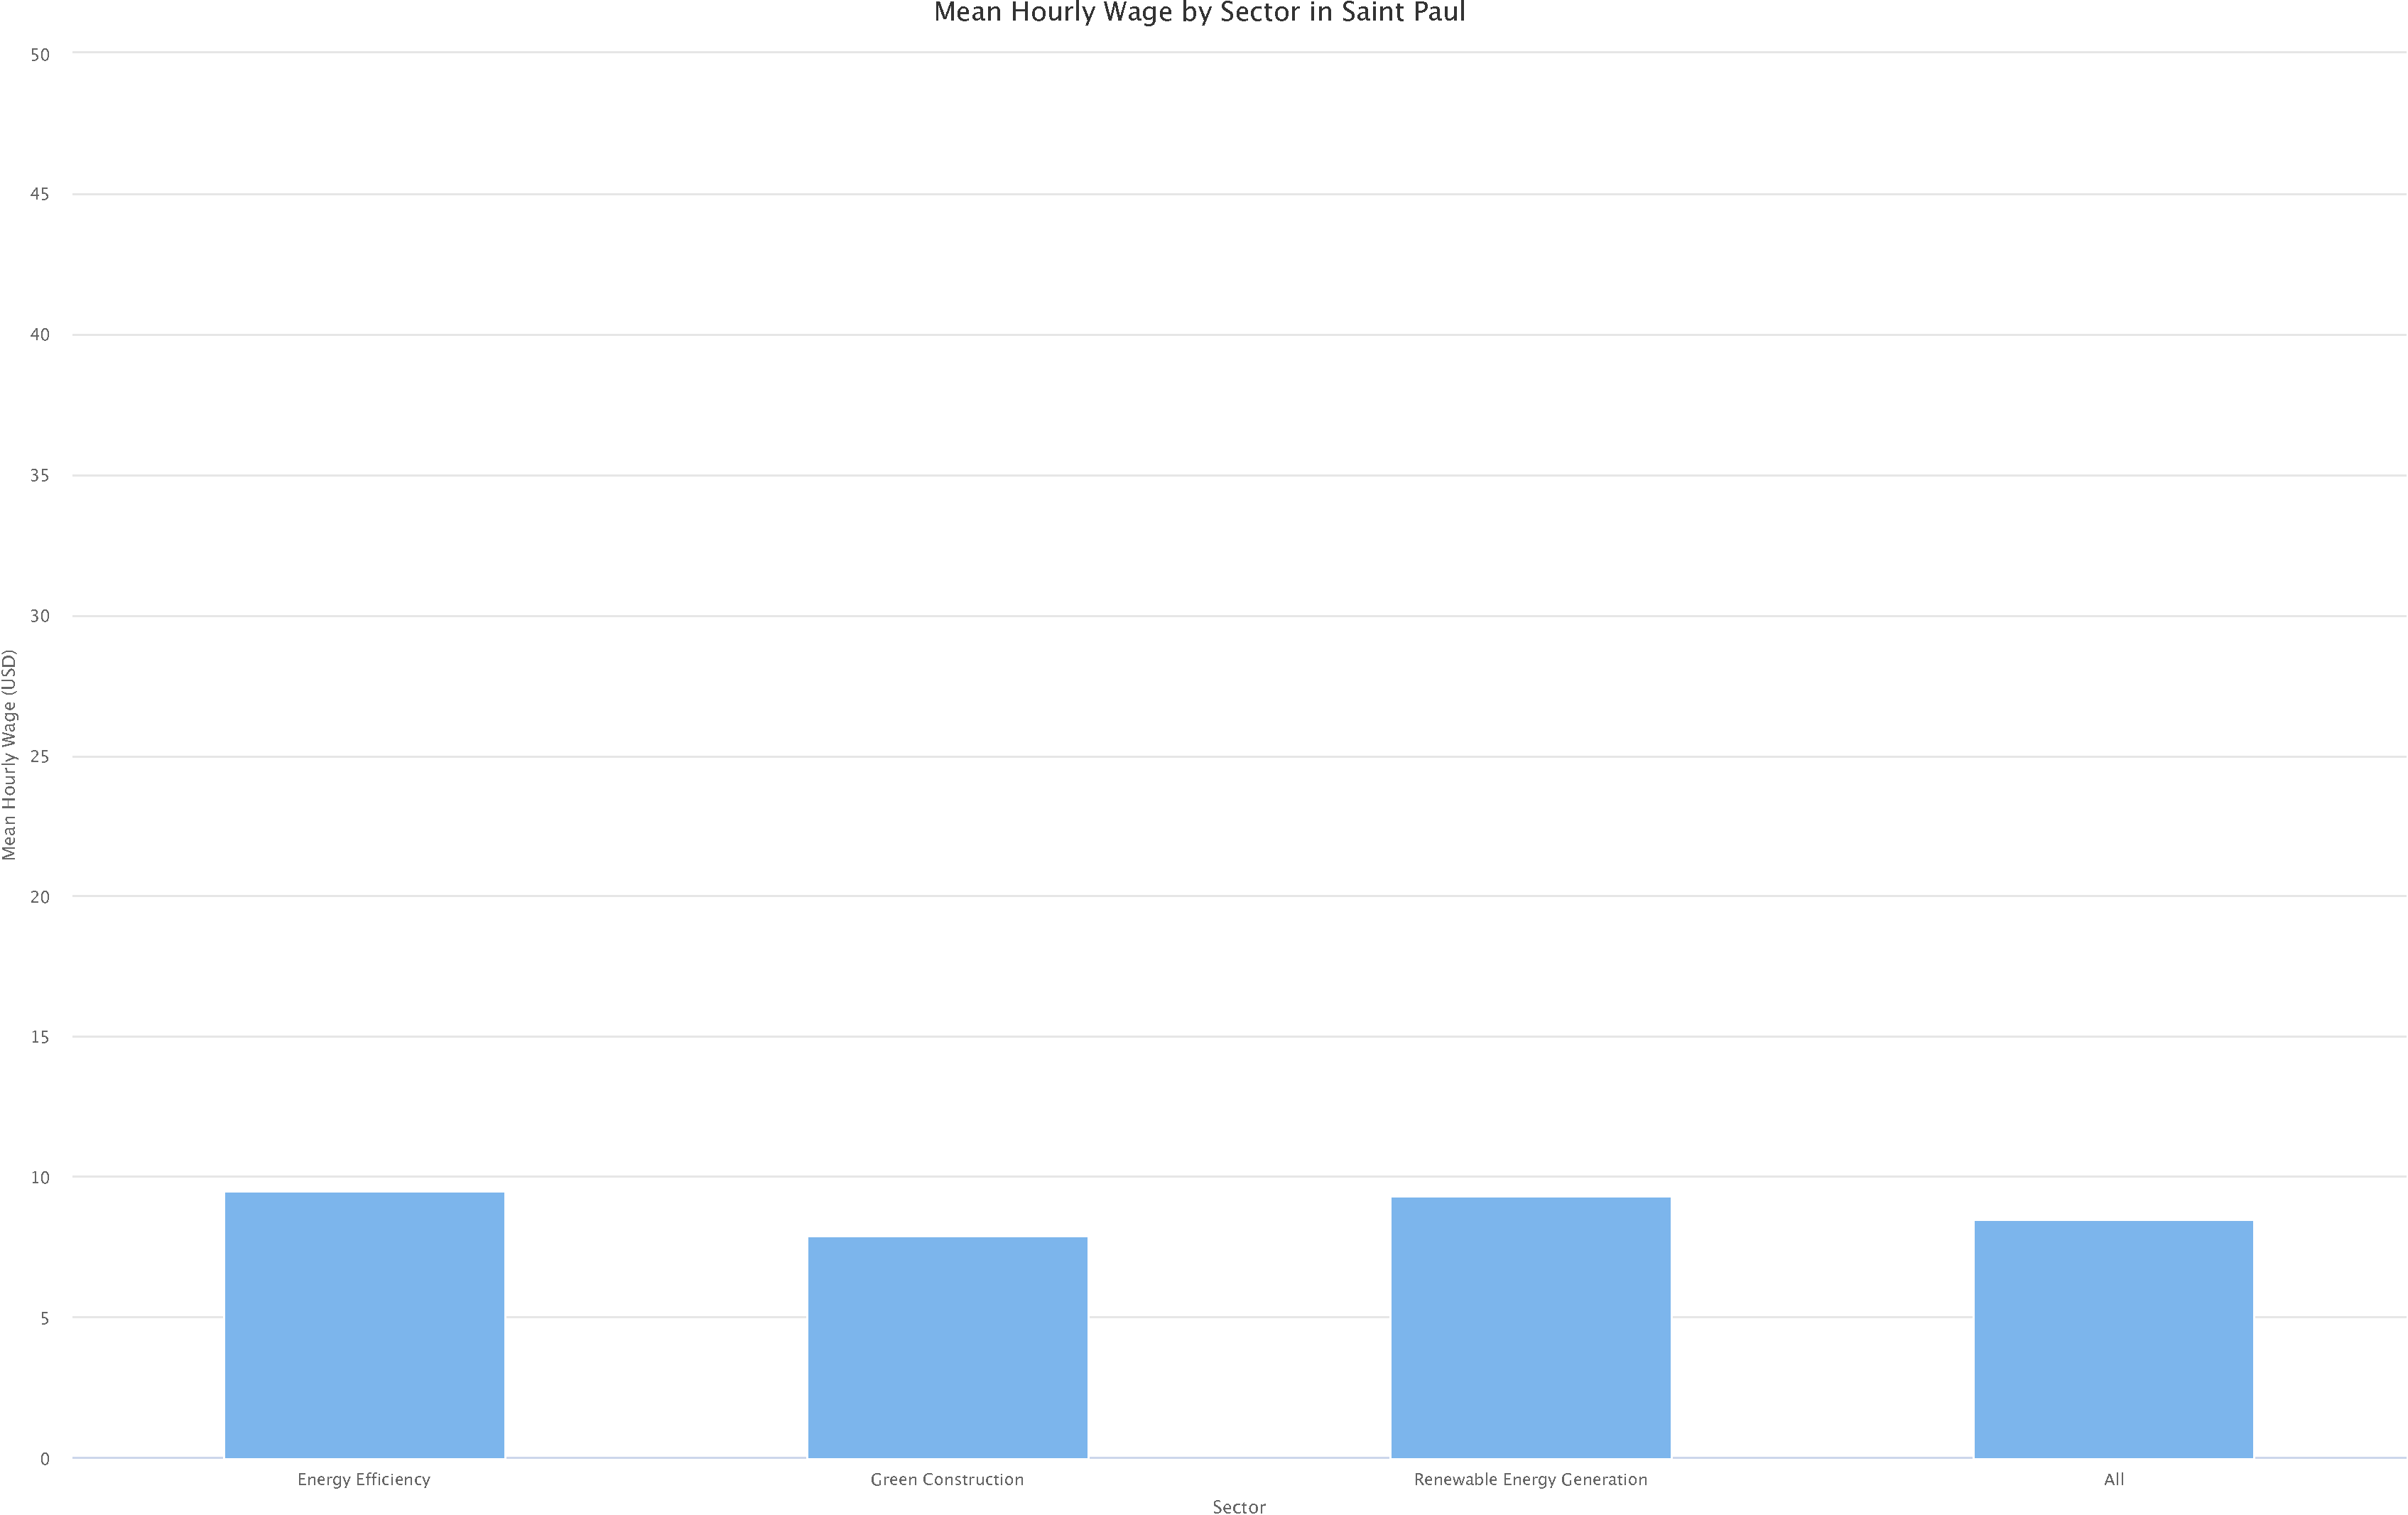
\includegraphics{index_files/figure-pdf/unnamed-chunk-21-2.pdf}

\begin{Shaded}
\begin{Highlighting}[]
\CommentTok{\# Visualizing A\_MEAN (Mean Annual Wage) across the sectors for St. Paul}
\FunctionTok{hchart}\NormalTok{(final\_summary\_st\_paul, }\StringTok{"column"}\NormalTok{, }\FunctionTok{hcaes}\NormalTok{(}\AttributeTok{x =} \StringTok{\textasciigrave{}}\AttributeTok{O*NET{-}SOC Sector}\StringTok{\textasciigrave{}}\NormalTok{, }\AttributeTok{y =}\NormalTok{ A\_MEAN)) }\SpecialCharTok{\%\textgreater{}\%}
  \FunctionTok{hc\_title}\NormalTok{(}\AttributeTok{text =} \StringTok{"Mean Annual Wage by Sector in Saint Paul"}\NormalTok{) }\SpecialCharTok{\%\textgreater{}\%}
  \FunctionTok{hc\_xAxis}\NormalTok{(}\AttributeTok{title =} \FunctionTok{list}\NormalTok{(}\AttributeTok{text =} \StringTok{"Sector"}\NormalTok{)) }\SpecialCharTok{\%\textgreater{}\%}
  \FunctionTok{hc\_yAxis}\NormalTok{(}\AttributeTok{title =} \FunctionTok{list}\NormalTok{(}\AttributeTok{text =} \StringTok{"Mean Annual Wage (USD)"}\NormalTok{), }\AttributeTok{labels =} \FunctionTok{list}\NormalTok{(}\AttributeTok{format =} \StringTok{"\{value:,0f\}"}\NormalTok{)) }\SpecialCharTok{\%\textgreater{}\%}
  \FunctionTok{hc\_tooltip}\NormalTok{(}\AttributeTok{pointFormat =} \StringTok{\textquotesingle{}\textless{}b\textgreater{}\{point.y:,0f\} USD\textless{}/b\textgreater{}\textquotesingle{}}\NormalTok{)}
\end{Highlighting}
\end{Shaded}

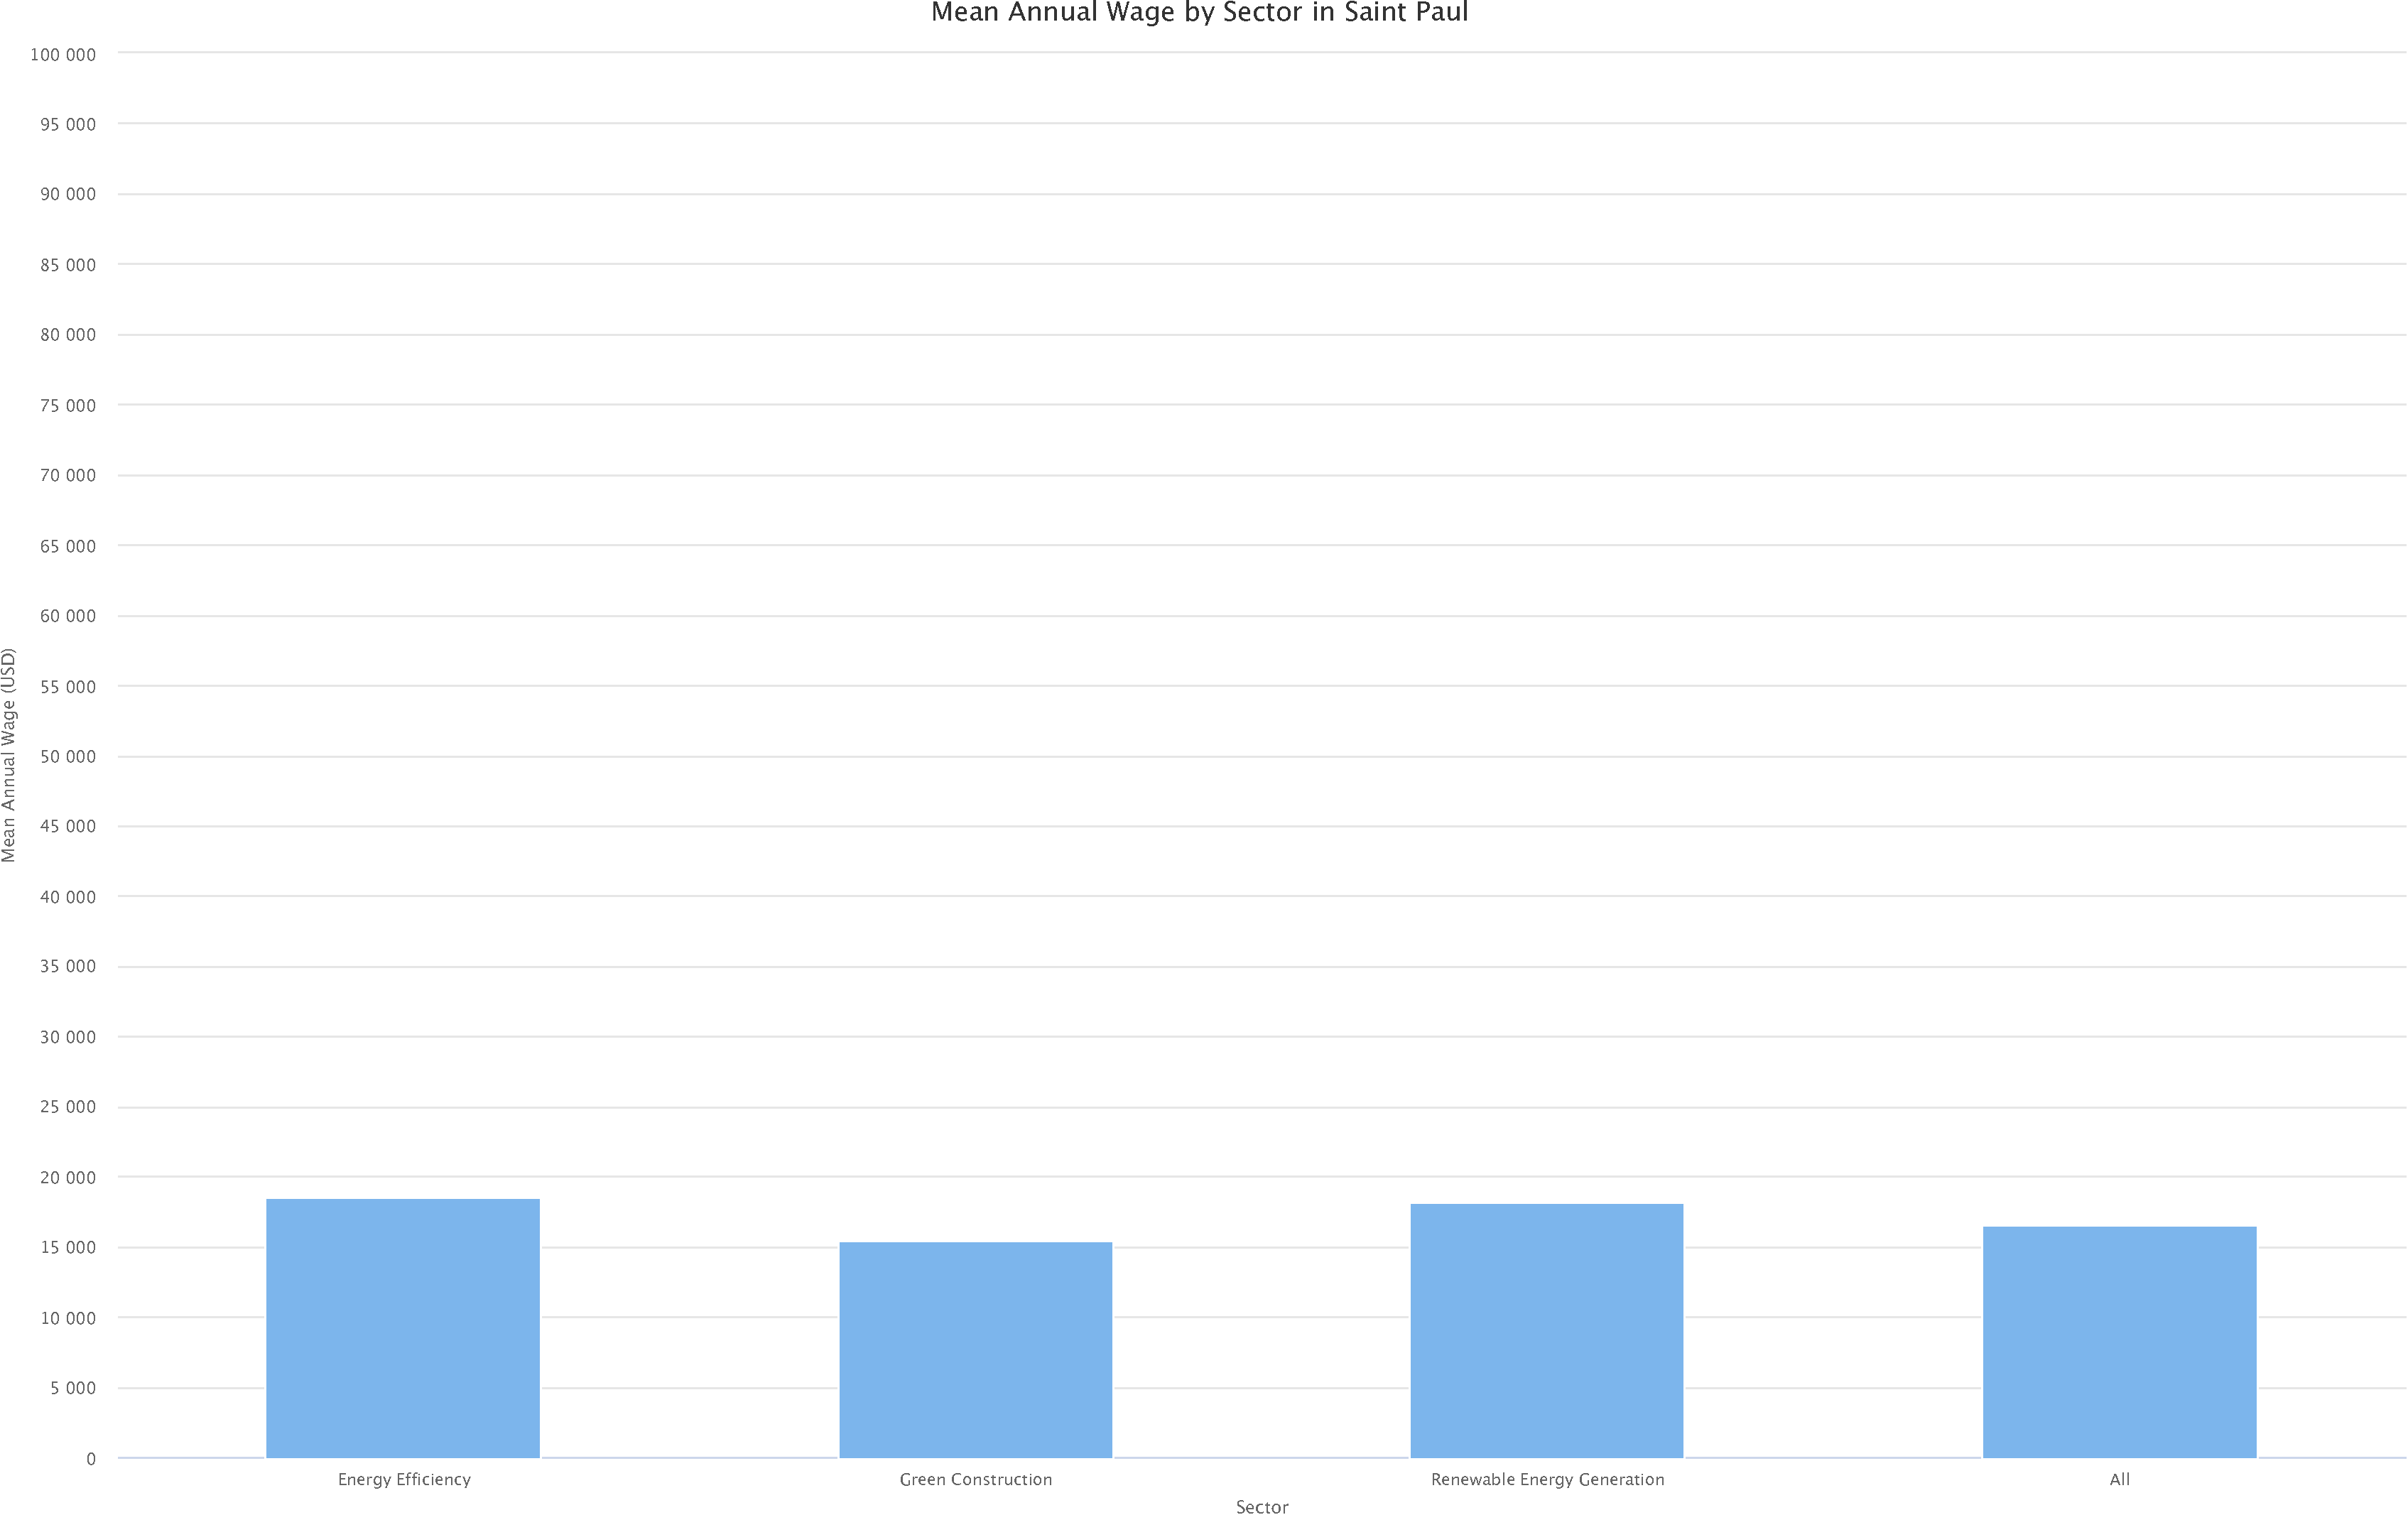
\includegraphics{index_files/figure-pdf/unnamed-chunk-21-3.pdf}

\begin{Shaded}
\begin{Highlighting}[]
\CommentTok{\# Visualizing A\_MEDIAN (Median Annual Wage) across the sectors for St. Paul}
\FunctionTok{hchart}\NormalTok{(final\_summary\_st\_paul, }\StringTok{"column"}\NormalTok{, }\FunctionTok{hcaes}\NormalTok{(}\AttributeTok{x =} \StringTok{\textasciigrave{}}\AttributeTok{O*NET{-}SOC Sector}\StringTok{\textasciigrave{}}\NormalTok{, }\AttributeTok{y =}\NormalTok{ A\_MEDIAN)) }\SpecialCharTok{\%\textgreater{}\%}
  \FunctionTok{hc\_title}\NormalTok{(}\AttributeTok{text =} \StringTok{"Median Annual Wage by Sector in Saint Paul"}\NormalTok{) }\SpecialCharTok{\%\textgreater{}\%}
  \FunctionTok{hc\_xAxis}\NormalTok{(}\AttributeTok{title =} \FunctionTok{list}\NormalTok{(}\AttributeTok{text =} \StringTok{"Sector"}\NormalTok{)) }\SpecialCharTok{\%\textgreater{}\%}
  \FunctionTok{hc\_yAxis}\NormalTok{(}\AttributeTok{title =} \FunctionTok{list}\NormalTok{(}\AttributeTok{text =} \StringTok{"Median Annual Wage (USD)"}\NormalTok{), }\AttributeTok{labels =} \FunctionTok{list}\NormalTok{(}\AttributeTok{format =} \StringTok{"\{value:,0f\}"}\NormalTok{)) }\SpecialCharTok{\%\textgreater{}\%}
  \FunctionTok{hc\_tooltip}\NormalTok{(}\AttributeTok{pointFormat =} \StringTok{\textquotesingle{}\textless{}b\textgreater{}\{point.y:,0f\} USD\textless{}/b\textgreater{}\textquotesingle{}}\NormalTok{)}
\end{Highlighting}
\end{Shaded}

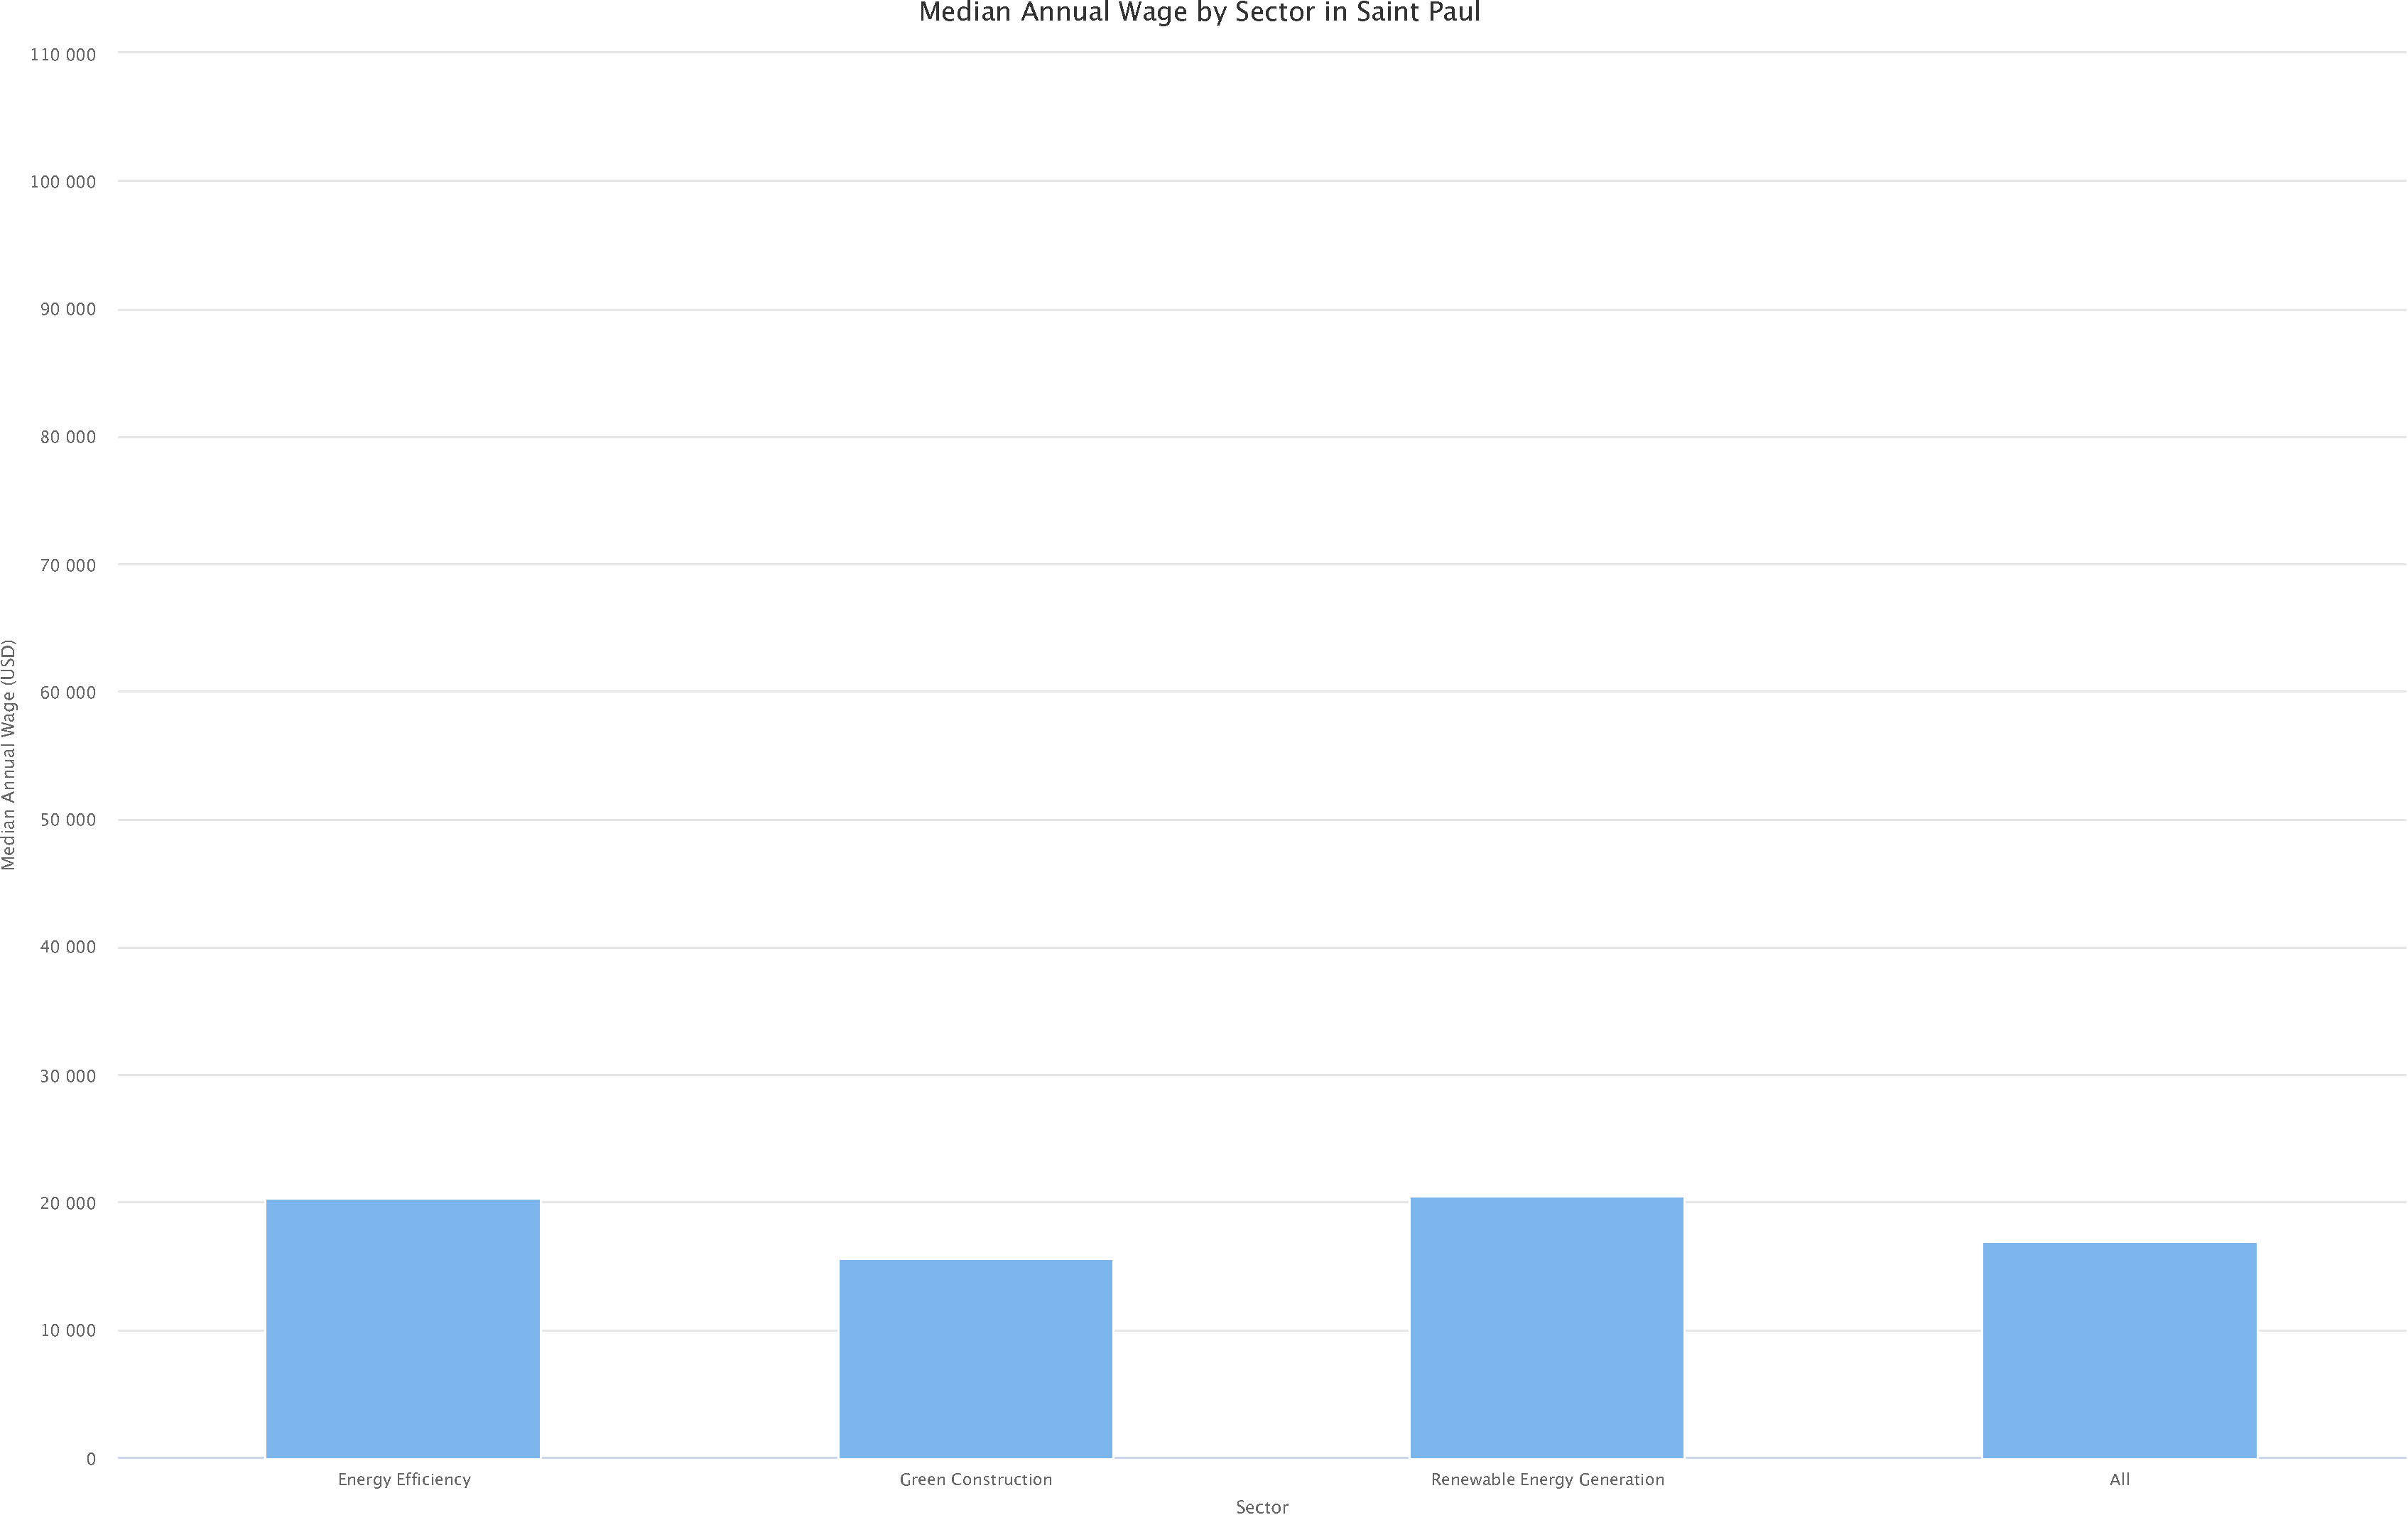
\includegraphics{index_files/figure-pdf/unnamed-chunk-21-4.pdf}

\begin{Shaded}
\begin{Highlighting}[]
\CommentTok{\# Visualizing H\_MEDIAN (Median Hourly Wage) across the sectors for St. Paul}
\FunctionTok{hchart}\NormalTok{(final\_summary\_st\_paul, }\StringTok{"column"}\NormalTok{, }\FunctionTok{hcaes}\NormalTok{(}\AttributeTok{x =} \StringTok{\textasciigrave{}}\AttributeTok{O*NET{-}SOC Sector}\StringTok{\textasciigrave{}}\NormalTok{, }\AttributeTok{y =}\NormalTok{ H\_MEDIAN)) }\SpecialCharTok{\%\textgreater{}\%}
  \FunctionTok{hc\_title}\NormalTok{(}\AttributeTok{text =} \StringTok{"Median Hourly Wage by Sector in Saint Paul"}\NormalTok{) }\SpecialCharTok{\%\textgreater{}\%}
  \FunctionTok{hc\_xAxis}\NormalTok{(}\AttributeTok{title =} \FunctionTok{list}\NormalTok{(}\AttributeTok{text =} \StringTok{"Sector"}\NormalTok{)) }\SpecialCharTok{\%\textgreater{}\%}
  \FunctionTok{hc\_yAxis}\NormalTok{(}\AttributeTok{title =} \FunctionTok{list}\NormalTok{(}\AttributeTok{text =} \StringTok{"Median Hourly Wage (USD)"}\NormalTok{)) }\SpecialCharTok{\%\textgreater{}\%}
  \FunctionTok{hc\_tooltip}\NormalTok{(}\AttributeTok{pointFormat =} \StringTok{\textquotesingle{}\textless{}b\textgreater{}\{point.y:.2f\} USD\textless{}/b\textgreater{}\textquotesingle{}}\NormalTok{)}
\end{Highlighting}
\end{Shaded}

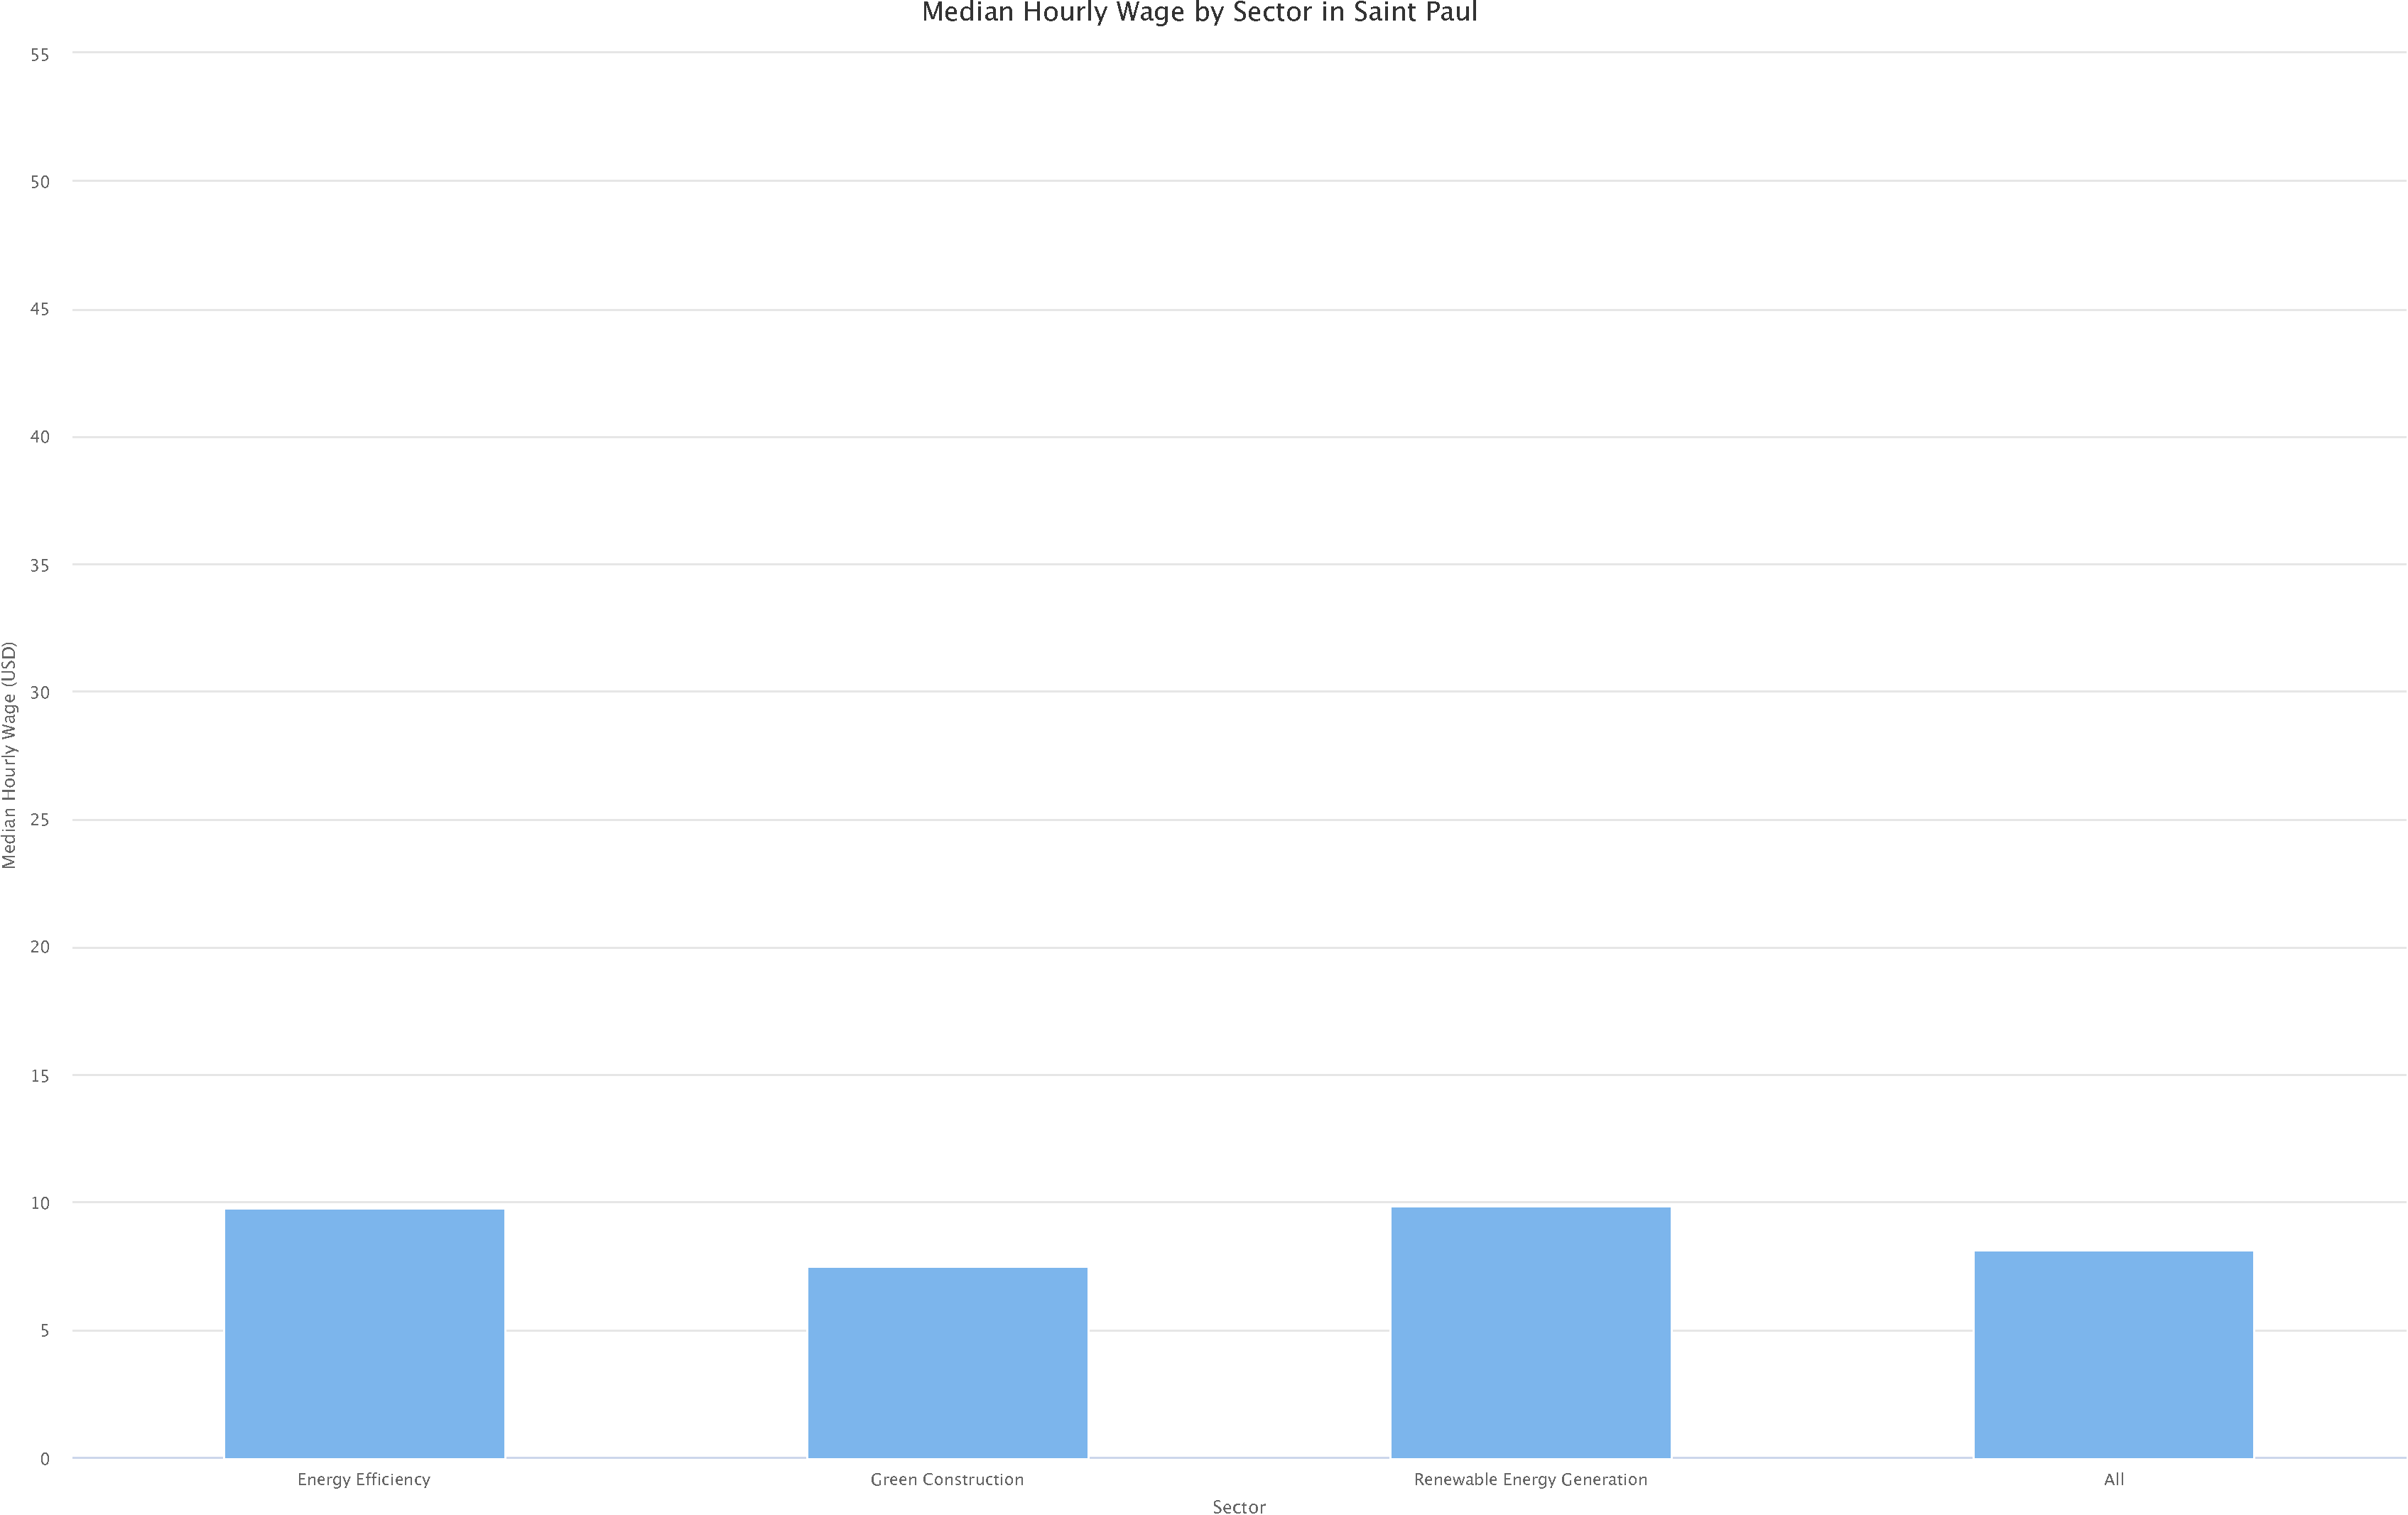
\includegraphics{index_files/figure-pdf/unnamed-chunk-21-5.pdf}

\begin{Shaded}
\begin{Highlighting}[]
\CommentTok{\# Define green jobs as sectors related to energy and construction for St. Paul}
\NormalTok{green\_jobs\_sectors\_st\_paul }\OtherTok{\textless{}{-}} \FunctionTok{c}\NormalTok{(}\StringTok{"Energy Efficiency"}\NormalTok{, }\StringTok{"Renewable Energy Generation"}\NormalTok{, }\StringTok{"Green Construction"}\NormalTok{)}

\CommentTok{\# Add a new column to identify green and non{-}green jobs for St. Paul}
\NormalTok{st\_paul\_jobs }\OtherTok{\textless{}{-}}\NormalTok{ st\_paul\_jobs }\SpecialCharTok{\%\textgreater{}\%}
  \FunctionTok{mutate}\NormalTok{(}
    \AttributeTok{Job\_Type =} \FunctionTok{ifelse}\NormalTok{(}\StringTok{\textasciigrave{}}\AttributeTok{O*NET{-}SOC Sector}\StringTok{\textasciigrave{}} \SpecialCharTok{\%in\%}\NormalTok{ green\_jobs\_sectors\_st\_paul, }\StringTok{"Green Jobs"}\NormalTok{, }\StringTok{"Non{-}Green Jobs"}\NormalTok{)}
\NormalTok{  )}

\CommentTok{\# Group by job type (Green vs Non{-}Green) and calculate mean wages for St. Paul}
\NormalTok{job\_type\_summary\_st\_paul }\OtherTok{\textless{}{-}}\NormalTok{ st\_paul\_jobs }\SpecialCharTok{\%\textgreater{}\%}
  \FunctionTok{group\_by}\NormalTok{(Job\_Type) }\SpecialCharTok{\%\textgreater{}\%}
  \FunctionTok{summarize}\NormalTok{(}
    \AttributeTok{H\_MEAN =} \FunctionTok{mean}\NormalTok{(H\_MEAN, }\AttributeTok{na.rm =} \ConstantTok{TRUE}\NormalTok{),}
    \AttributeTok{A\_MEAN =} \FunctionTok{mean}\NormalTok{(A\_MEAN, }\AttributeTok{na.rm =} \ConstantTok{TRUE}\NormalTok{)}
\NormalTok{  )}

\CommentTok{\# Visualizing Mean Hourly Wage (H\_MEAN) for Green vs Non{-}Green Jobs in St. Paul}
\FunctionTok{hchart}\NormalTok{(job\_type\_summary\_st\_paul, }\StringTok{"column"}\NormalTok{, }\FunctionTok{hcaes}\NormalTok{(}\AttributeTok{x =}\NormalTok{ Job\_Type, }\AttributeTok{y =}\NormalTok{ H\_MEAN)) }\SpecialCharTok{\%\textgreater{}\%}
  \FunctionTok{hc\_title}\NormalTok{(}\AttributeTok{text =} \StringTok{"Mean Hourly Wage: Green Jobs vs Non{-}Green Jobs in Saint Paul"}\NormalTok{) }\SpecialCharTok{\%\textgreater{}\%}
  \FunctionTok{hc\_xAxis}\NormalTok{(}\AttributeTok{title =} \FunctionTok{list}\NormalTok{(}\AttributeTok{text =} \StringTok{"Job Type"}\NormalTok{)) }\SpecialCharTok{\%\textgreater{}\%}
  \FunctionTok{hc\_yAxis}\NormalTok{(}\AttributeTok{title =} \FunctionTok{list}\NormalTok{(}\AttributeTok{text =} \StringTok{"Mean Hourly Wage (USD)"}\NormalTok{)) }\SpecialCharTok{\%\textgreater{}\%}
  \FunctionTok{hc\_tooltip}\NormalTok{(}\AttributeTok{pointFormat =} \StringTok{\textquotesingle{}\textless{}b\textgreater{}\{point.y:.2f\} USD\textless{}/b\textgreater{}\textquotesingle{}}\NormalTok{)}
\end{Highlighting}
\end{Shaded}

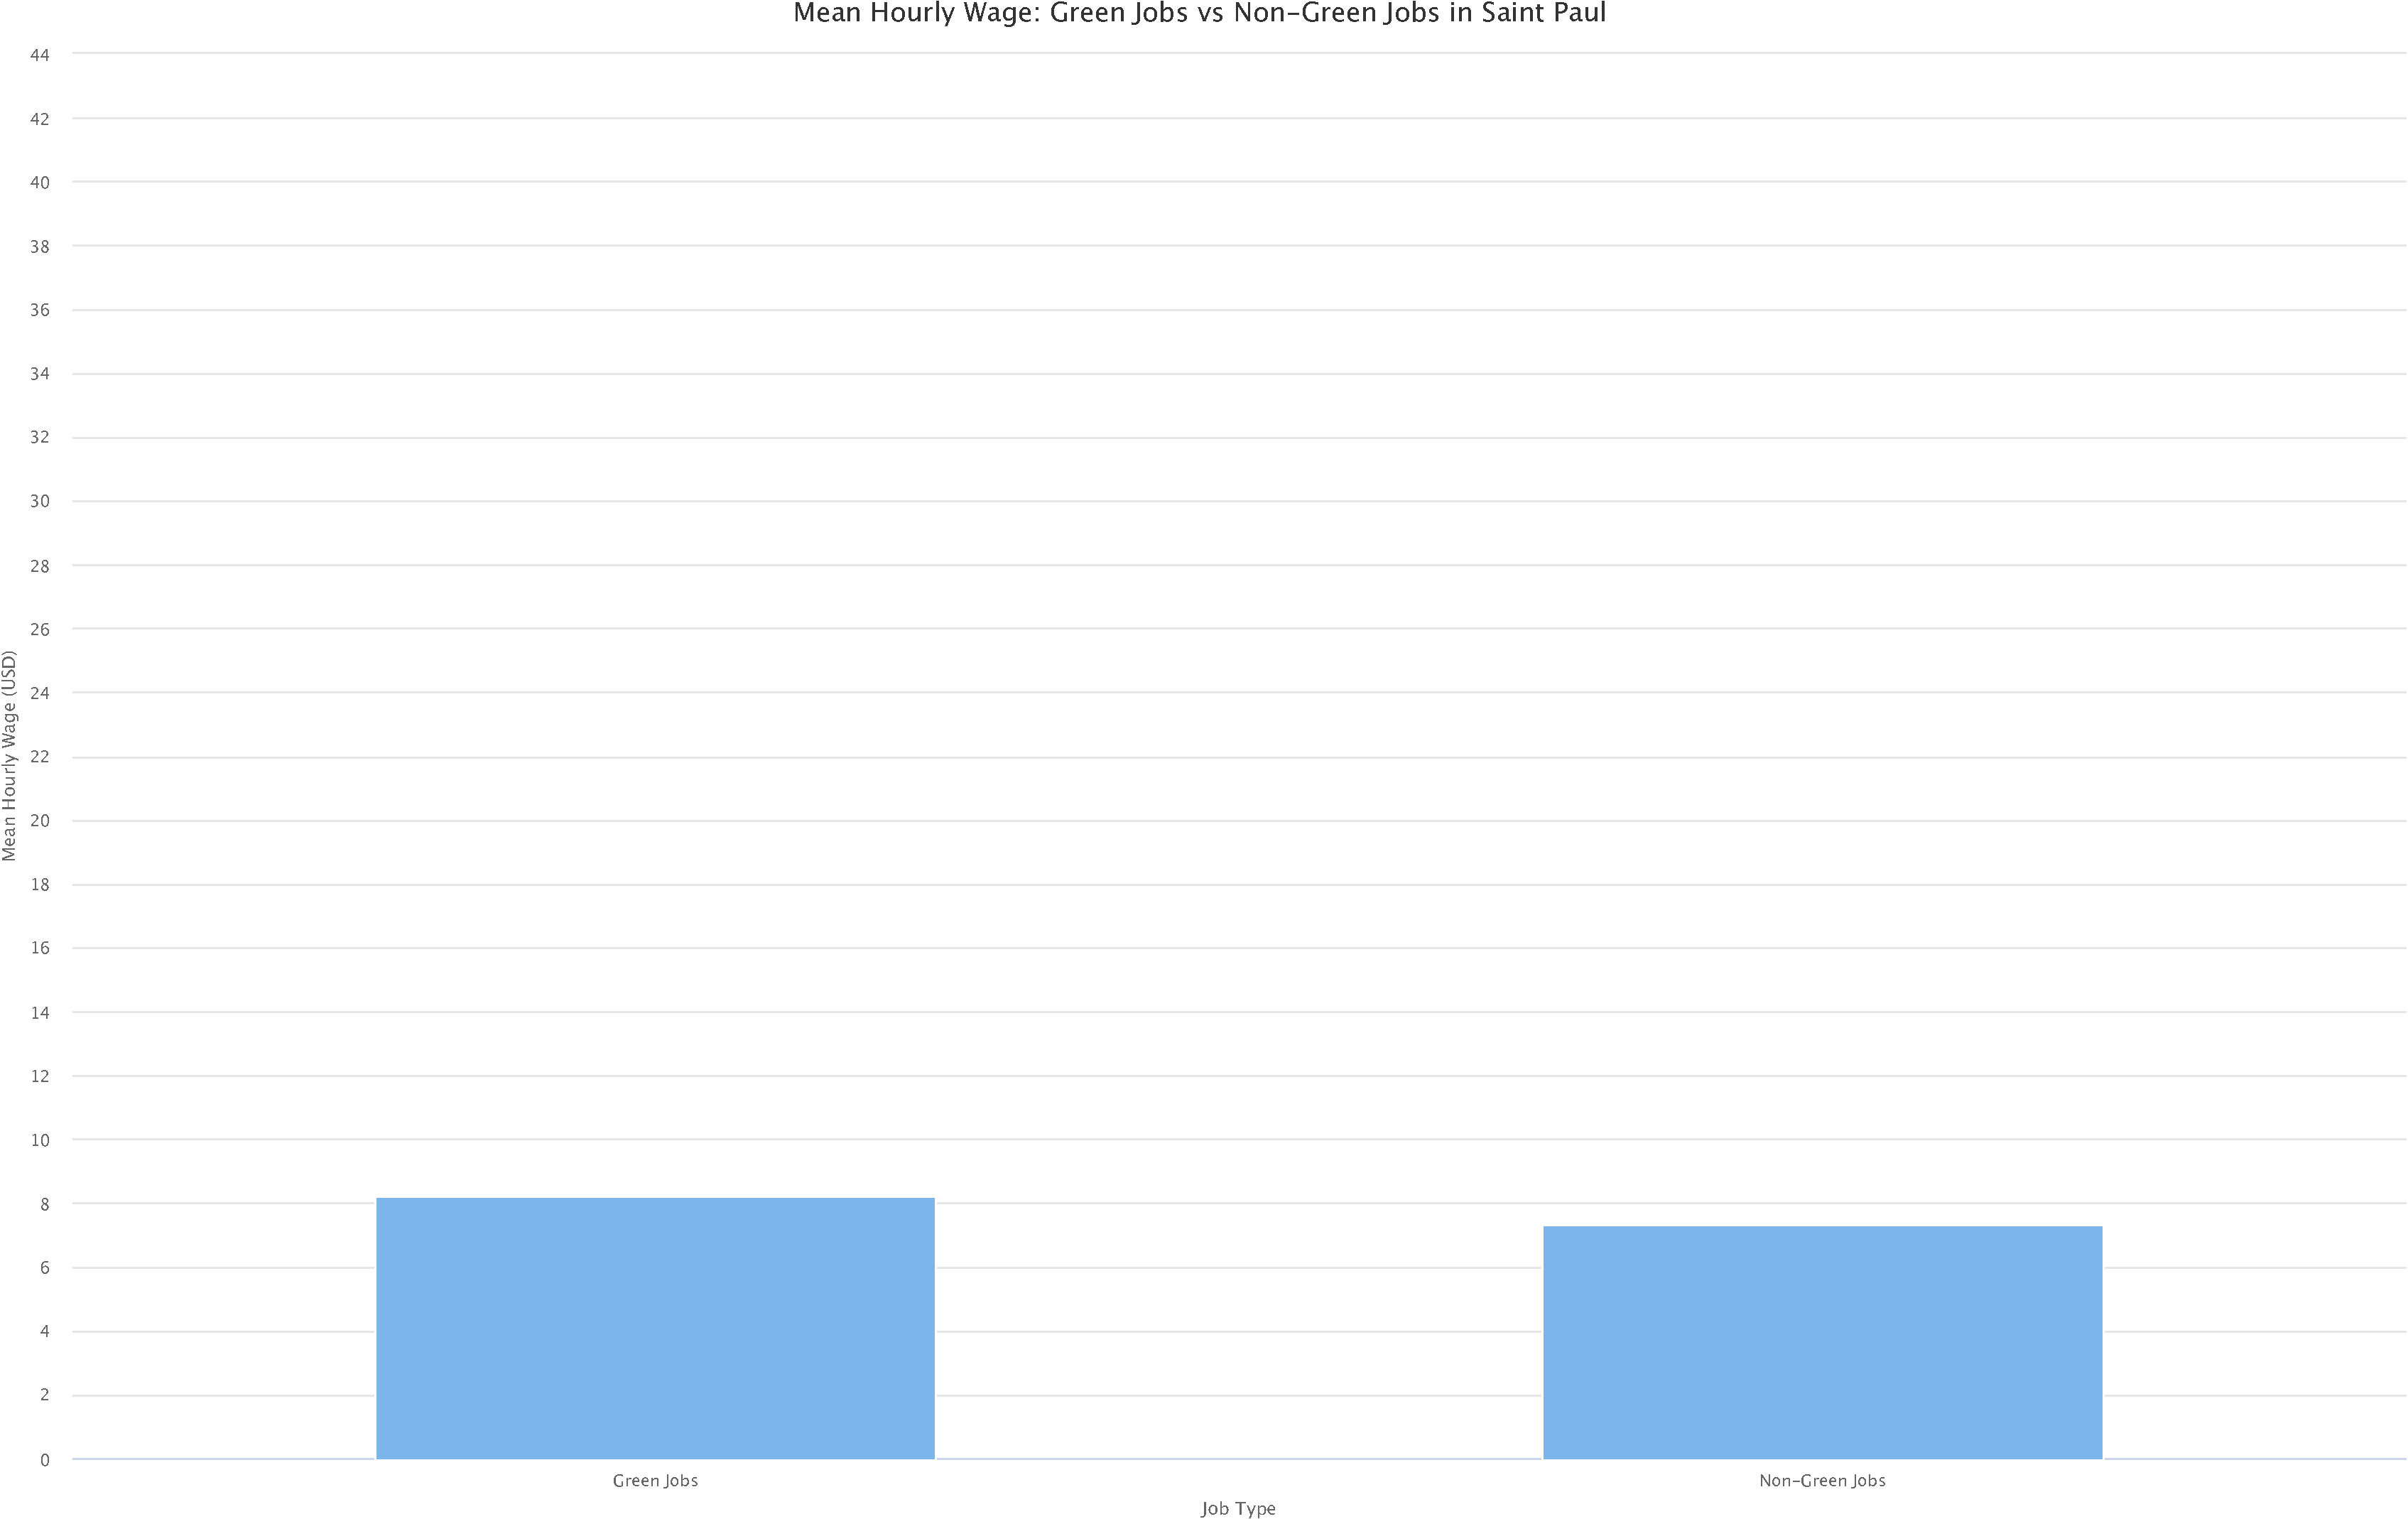
\includegraphics{index_files/figure-pdf/unnamed-chunk-21-6.pdf}

\begin{Shaded}
\begin{Highlighting}[]
\CommentTok{\# Visualizing Mean Annual Wage (A\_MEAN) for Green vs Non{-}Green Jobs in St. Paul}
\FunctionTok{hchart}\NormalTok{(job\_type\_summary\_st\_paul, }\StringTok{"column"}\NormalTok{, }\FunctionTok{hcaes}\NormalTok{(}\AttributeTok{x =}\NormalTok{ Job\_Type, }\AttributeTok{y =}\NormalTok{ A\_MEAN)) }\SpecialCharTok{\%\textgreater{}\%}
  \FunctionTok{hc\_title}\NormalTok{(}\AttributeTok{text =} \StringTok{"Mean Annual Wage: Green Jobs vs Non{-}Green Jobs in Saint Paul"}\NormalTok{) }\SpecialCharTok{\%\textgreater{}\%}
  \FunctionTok{hc\_xAxis}\NormalTok{(}\AttributeTok{title =} \FunctionTok{list}\NormalTok{(}\AttributeTok{text =} \StringTok{"Job Type"}\NormalTok{)) }\SpecialCharTok{\%\textgreater{}\%}
  \FunctionTok{hc\_yAxis}\NormalTok{(}\AttributeTok{title =} \FunctionTok{list}\NormalTok{(}\AttributeTok{text =} \StringTok{"Mean Annual Wage (USD)"}\NormalTok{)) }\SpecialCharTok{\%\textgreater{}\%}
  \FunctionTok{hc\_tooltip}\NormalTok{(}\AttributeTok{pointFormat =} \StringTok{\textquotesingle{}\textless{}b\textgreater{}\{point.y:,0f\} USD\textless{}/b\textgreater{}\textquotesingle{}}\NormalTok{)}
\end{Highlighting}
\end{Shaded}

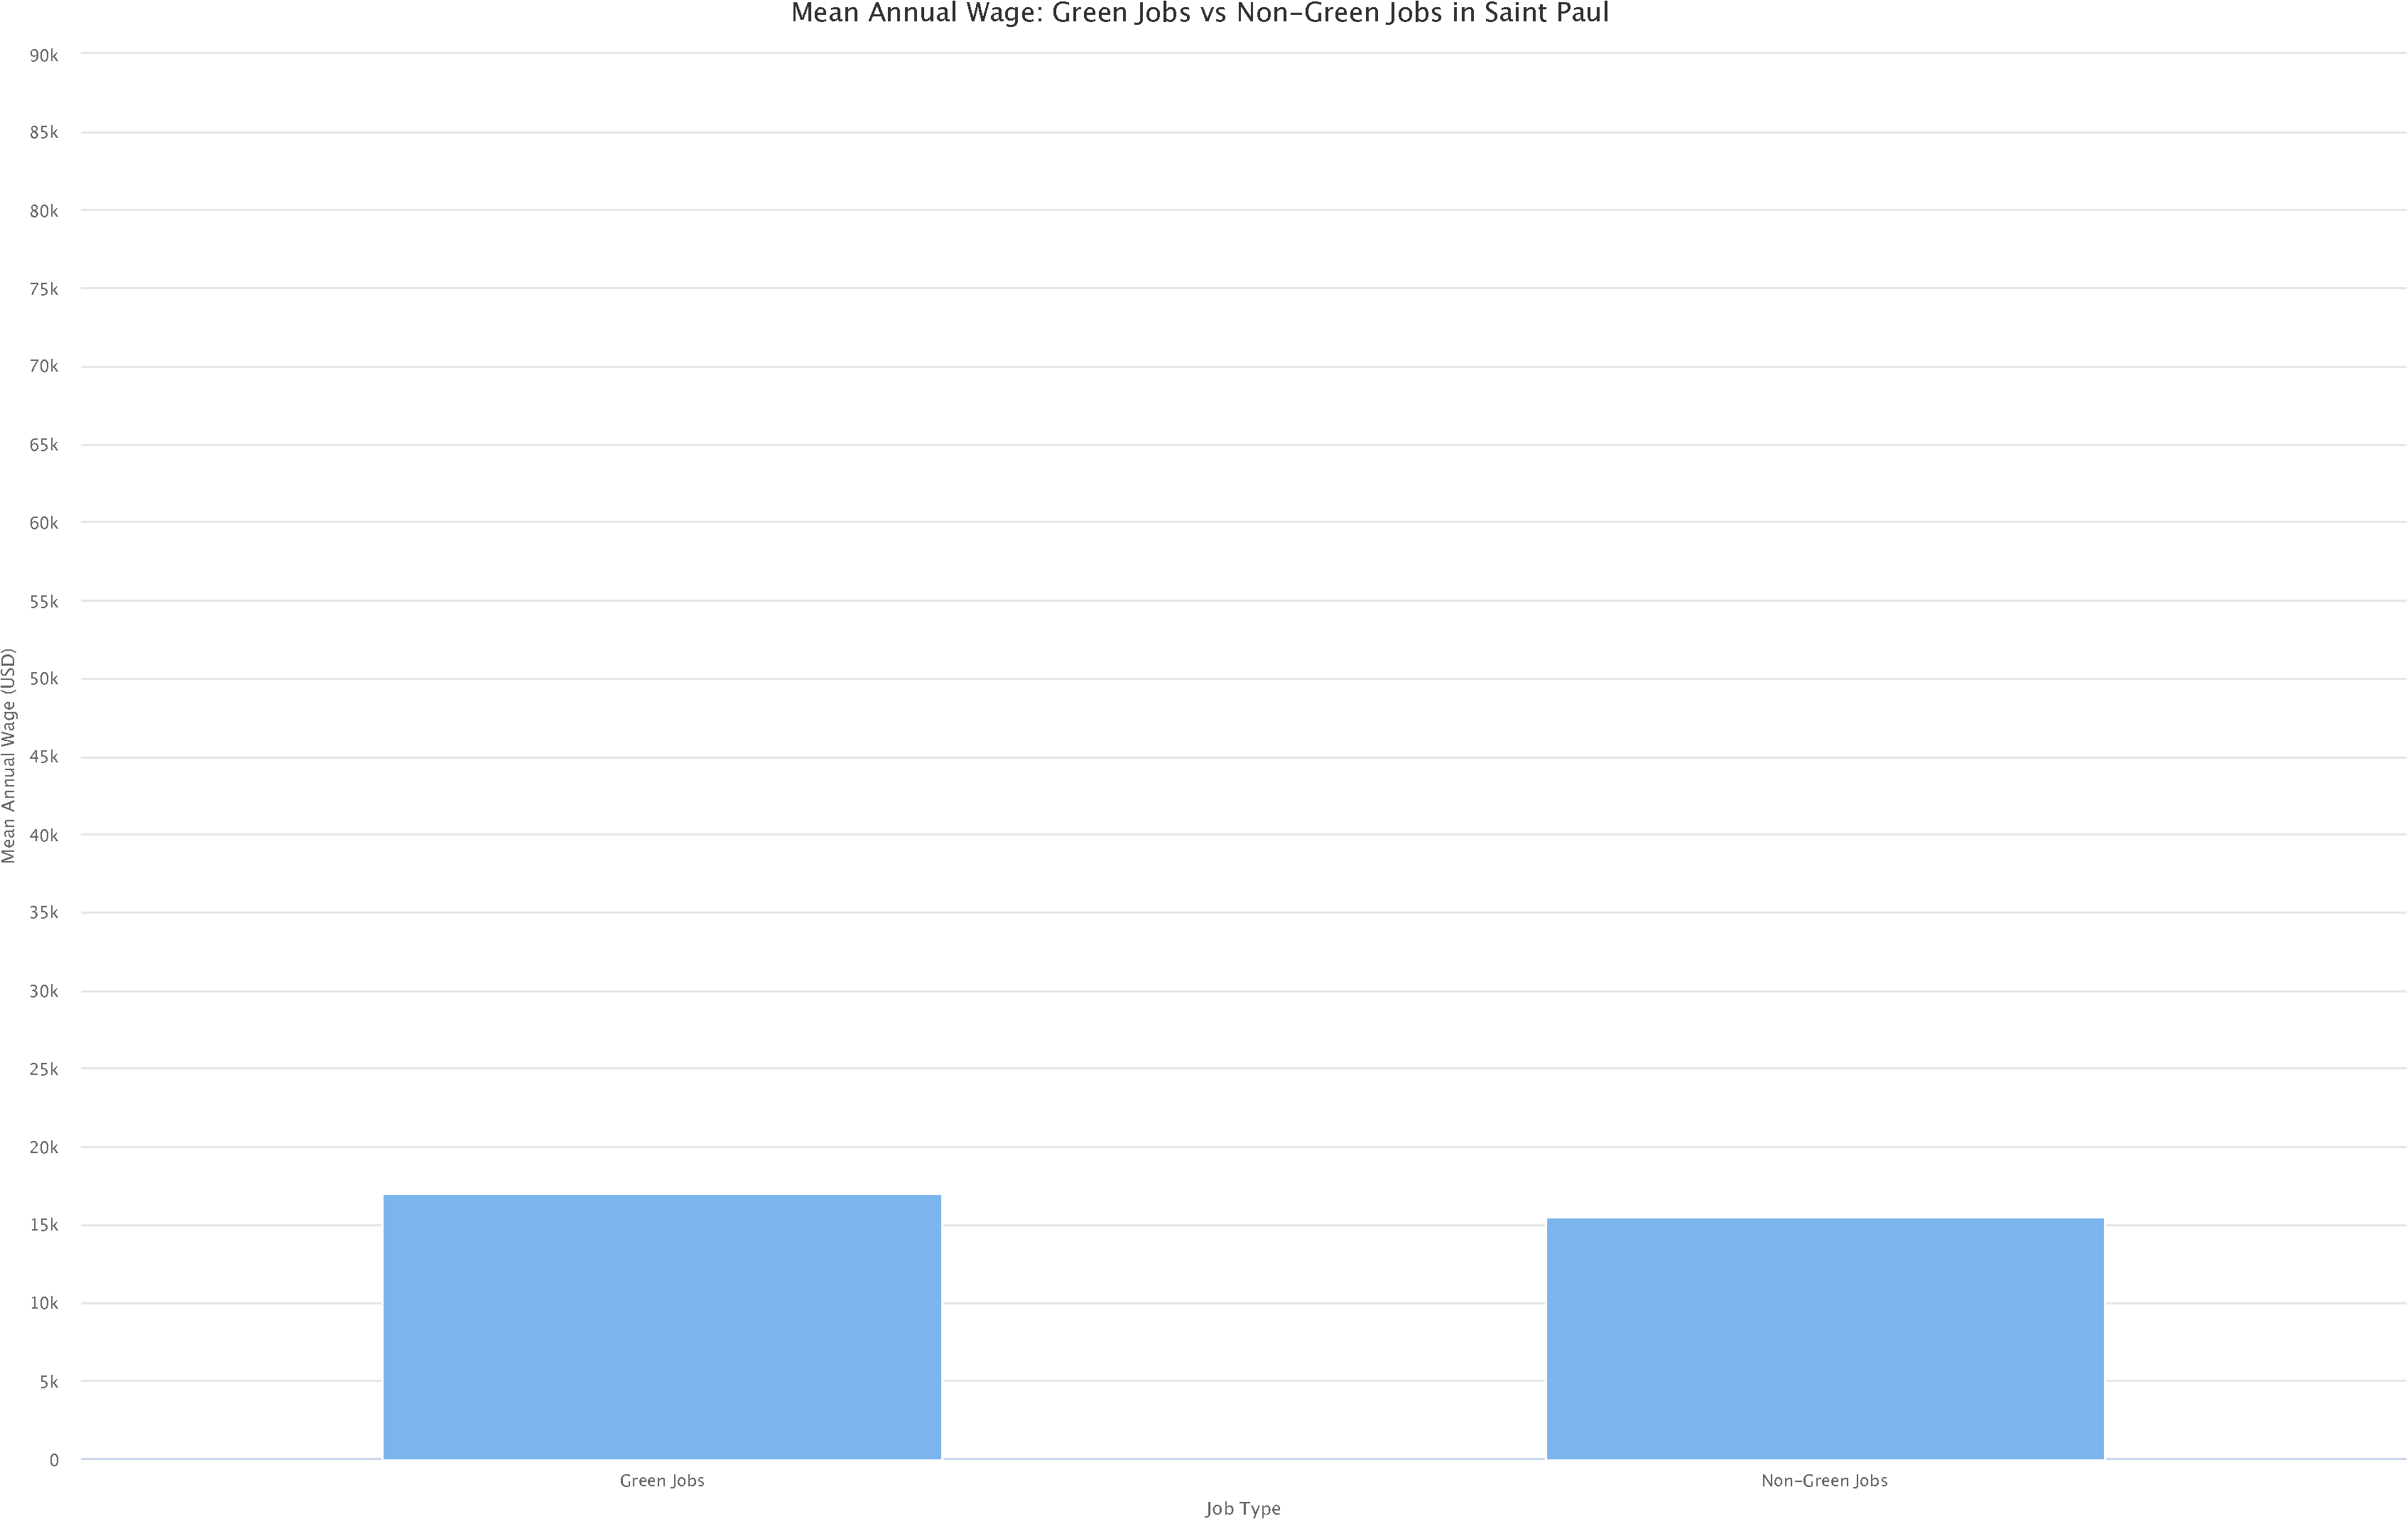
\includegraphics{index_files/figure-pdf/unnamed-chunk-21-7.pdf}

\begin{Shaded}
\begin{Highlighting}[]
\CommentTok{\# Summarizing core findings for Saint Paul}

\CommentTok{\# Extract green and non{-}green job wage data for St. Paul}
\NormalTok{green\_wages\_st\_paul }\OtherTok{\textless{}{-}}\NormalTok{ job\_type\_summary\_st\_paul }\SpecialCharTok{\%\textgreater{}\%} \FunctionTok{filter}\NormalTok{(Job\_Type }\SpecialCharTok{==} \StringTok{"Green Jobs"}\NormalTok{)}
\NormalTok{non\_green\_wages\_st\_paul }\OtherTok{\textless{}{-}}\NormalTok{ job\_type\_summary\_st\_paul }\SpecialCharTok{\%\textgreater{}\%} \FunctionTok{filter}\NormalTok{(Job\_Type }\SpecialCharTok{==} \StringTok{"Non{-}Green Jobs"}\NormalTok{)}

\CommentTok{\# Calculate the difference between green and non{-}green jobs for St. Paul}
\NormalTok{difference\_annual\_st\_paul }\OtherTok{\textless{}{-}}\NormalTok{ green\_wages\_st\_paul}\SpecialCharTok{$}\NormalTok{A\_MEAN }\SpecialCharTok{{-}}\NormalTok{ non\_green\_wages\_st\_paul}\SpecialCharTok{$}\NormalTok{A\_MEAN}
\NormalTok{difference\_hourly\_st\_paul }\OtherTok{\textless{}{-}}\NormalTok{ green\_wages\_st\_paul}\SpecialCharTok{$}\NormalTok{H\_MEAN }\SpecialCharTok{{-}}\NormalTok{ non\_green\_wages\_st\_paul}\SpecialCharTok{$}\NormalTok{H\_MEAN}

\CommentTok{\# Format and print the sentences for Saint Paul}
\FunctionTok{cat}\NormalTok{(}\StringTok{"The mean annual wage for the occupation in U.S. dollars for green jobs in Saint Paul is $"}\NormalTok{, }
    \FunctionTok{format}\NormalTok{(green\_wages\_st\_paul}\SpecialCharTok{$}\NormalTok{A\_MEAN, }\AttributeTok{big.mark =} \StringTok{","}\NormalTok{, }\AttributeTok{scientific =} \ConstantTok{FALSE}\NormalTok{), }
    \StringTok{", and for non{-}green jobs is $"}\NormalTok{, }
    \FunctionTok{format}\NormalTok{(non\_green\_wages\_st\_paul}\SpecialCharTok{$}\NormalTok{A\_MEAN, }\AttributeTok{big.mark =} \StringTok{","}\NormalTok{, }\AttributeTok{scientific =} \ConstantTok{FALSE}\NormalTok{), }
    \StringTok{". That means green jobs in Saint Paul pay $"}\NormalTok{, }
    \FunctionTok{format}\NormalTok{(}\FunctionTok{abs}\NormalTok{(difference\_annual\_st\_paul), }\AttributeTok{big.mark =} \StringTok{","}\NormalTok{, }\AttributeTok{scientific =} \ConstantTok{FALSE}\NormalTok{), }
    \FunctionTok{ifelse}\NormalTok{(difference\_annual\_st\_paul }\SpecialCharTok{\textgreater{}} \DecValTok{0}\NormalTok{, }\StringTok{" more"}\NormalTok{, }\StringTok{" less"}\NormalTok{), }
    \StringTok{" than non{-}green jobs in Saint Paul.}\SpecialCharTok{\textbackslash{}n}\StringTok{"}\NormalTok{, }\AttributeTok{sep =} \StringTok{""}\NormalTok{)}
\end{Highlighting}
\end{Shaded}

\begin{verbatim}
The mean annual wage for the occupation in U.S. dollars for green jobs in Saint Paul is $84,561.7, and for non-green jobs is $77,192.53. That means green jobs in Saint Paul pay $7,369.169 more than non-green jobs in Saint Paul.
\end{verbatim}

\begin{Shaded}
\begin{Highlighting}[]
\FunctionTok{cat}\NormalTok{(}\StringTok{"The mean hourly wage for the occupation in U.S. dollars for green jobs in Saint Paul is $"}\NormalTok{, }
    \FunctionTok{format}\NormalTok{(green\_wages\_st\_paul}\SpecialCharTok{$}\NormalTok{H\_MEAN, }\AttributeTok{big.mark =} \StringTok{","}\NormalTok{, }\AttributeTok{scientific =} \ConstantTok{FALSE}\NormalTok{), }
    \StringTok{", and for non{-}green jobs is $"}\NormalTok{, }
    \FunctionTok{format}\NormalTok{(non\_green\_wages\_st\_paul}\SpecialCharTok{$}\NormalTok{H\_MEAN, }\AttributeTok{big.mark =} \StringTok{","}\NormalTok{, }\AttributeTok{scientific =} \ConstantTok{FALSE}\NormalTok{), }
    \StringTok{". That means green jobs in Saint Paul pay $"}\NormalTok{, }
    \FunctionTok{format}\NormalTok{(}\FunctionTok{abs}\NormalTok{(difference\_hourly\_st\_paul), }\AttributeTok{big.mark =} \StringTok{","}\NormalTok{, }\AttributeTok{scientific =} \ConstantTok{FALSE}\NormalTok{), }
    \FunctionTok{ifelse}\NormalTok{(difference\_hourly\_st\_paul }\SpecialCharTok{\textgreater{}} \DecValTok{0}\NormalTok{, }\StringTok{" more"}\NormalTok{, }\StringTok{" less"}\NormalTok{), }
    \StringTok{" than non{-}green jobs in Saint Paul.}\SpecialCharTok{\textbackslash{}n}\StringTok{"}\NormalTok{, }\AttributeTok{sep =} \StringTok{""}\NormalTok{)}
\end{Highlighting}
\end{Shaded}

\begin{verbatim}
The mean hourly wage for the occupation in U.S. dollars for green jobs in Saint Paul is $40.65447, and for non-green jobs is $36.30688. That means green jobs in Saint Paul pay $4.347591 more than non-green jobs in Saint Paul.
\end{verbatim}

\textsubscript{Source:
\href{https://beeckcenter.github.io/climate-equity-workforce/index-preview.html}{Article
Notebook}}

I'd like to see a word cloud of different job titles for each sector in
St.~Paul

\begin{Shaded}
\begin{Highlighting}[]
\CommentTok{\# Filter the dataset for green jobs only in St. Paul}
\NormalTok{green\_jobs\_st\_paul }\OtherTok{\textless{}{-}}\NormalTok{ st\_paul\_jobs }\SpecialCharTok{\%\textgreater{}\%}
  \FunctionTok{filter}\NormalTok{(}\StringTok{\textasciigrave{}}\AttributeTok{O*NET{-}SOC Sector}\StringTok{\textasciigrave{}} \SpecialCharTok{\%in\%} \FunctionTok{c}\NormalTok{(}\StringTok{"Energy Efficiency"}\NormalTok{, }\StringTok{"Renewable Energy Generation"}\NormalTok{, }\StringTok{"Green Construction"}\NormalTok{))}

\CommentTok{\# Extract job titles and count their occurrences in St. Paul}
\NormalTok{job\_titles\_st\_paul }\OtherTok{\textless{}{-}}\NormalTok{ green\_jobs\_st\_paul }\SpecialCharTok{\%\textgreater{}\%}
  \FunctionTok{count}\NormalTok{(OCC\_TITLE, }\AttributeTok{sort =} \ConstantTok{TRUE}\NormalTok{)}

\CommentTok{\# Create a word cloud for green jobs in St. Paul using highcharter}
\FunctionTok{hchart}\NormalTok{(}
\NormalTok{  job\_titles\_st\_paul, }
  \StringTok{"wordcloud"}\NormalTok{, }
  \FunctionTok{hcaes}\NormalTok{(}\AttributeTok{name =}\NormalTok{ OCC\_TITLE, }\AttributeTok{weight =}\NormalTok{ n)}
\NormalTok{) }\SpecialCharTok{\%\textgreater{}\%}
  \FunctionTok{hc\_title}\NormalTok{(}\AttributeTok{text =} \StringTok{"Word Cloud of Green Job Titles in Saint Paul"}\NormalTok{)}
\end{Highlighting}
\end{Shaded}

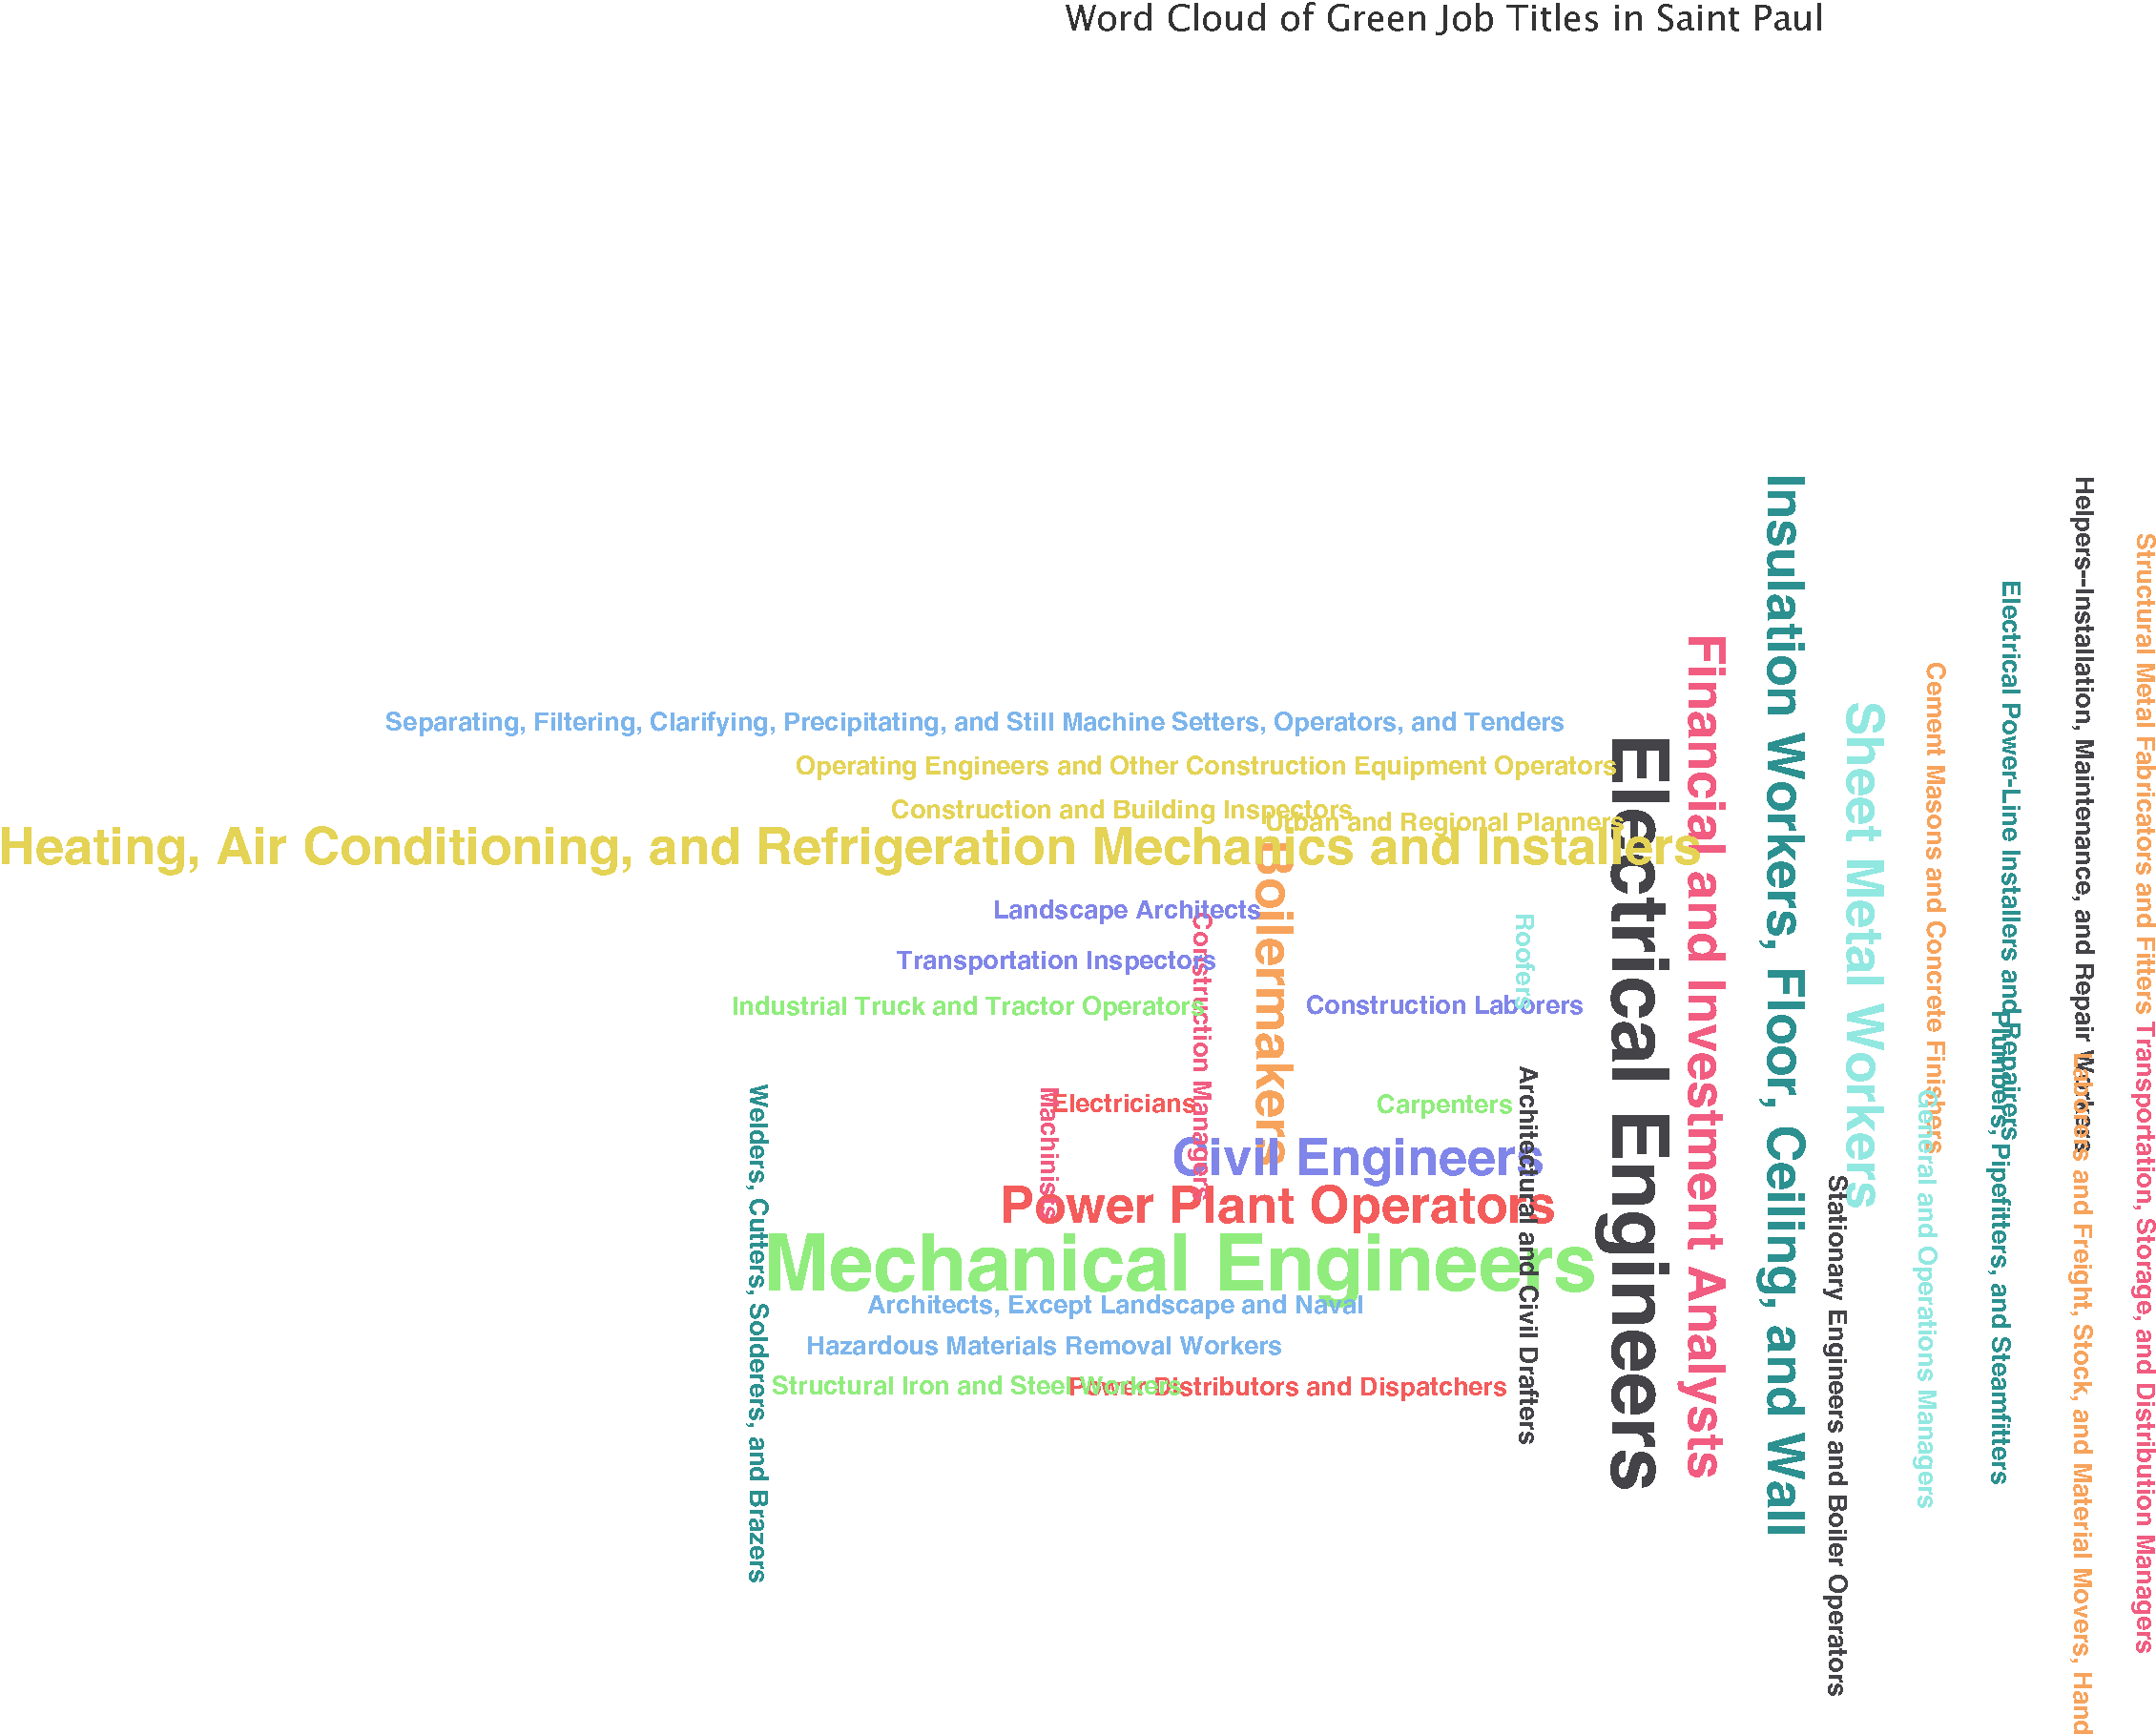
\includegraphics{index_files/figure-pdf/unnamed-chunk-22-1.pdf}

\textsubscript{Source:
\href{https://beeckcenter.github.io/climate-equity-workforce/index-preview.html}{Article
Notebook}}

Now let's create separate word clouds for each of the green sectors
(``Energy Efficiency'', ``Renewable Energy Generation'', and ``Green
Construction'') for St.~Paul

\begin{Shaded}
\begin{Highlighting}[]
\CommentTok{\# Filter the dataset for each sector in St. Paul}
\NormalTok{energy\_efficiency\_jobs\_st\_paul }\OtherTok{\textless{}{-}}\NormalTok{ st\_paul\_jobs }\SpecialCharTok{\%\textgreater{}\%}
  \FunctionTok{filter}\NormalTok{(}\StringTok{\textasciigrave{}}\AttributeTok{O*NET{-}SOC Sector}\StringTok{\textasciigrave{}} \SpecialCharTok{==} \StringTok{"Energy Efficiency"}\NormalTok{)}

\NormalTok{renewable\_energy\_jobs\_st\_paul }\OtherTok{\textless{}{-}}\NormalTok{ st\_paul\_jobs }\SpecialCharTok{\%\textgreater{}\%}
  \FunctionTok{filter}\NormalTok{(}\StringTok{\textasciigrave{}}\AttributeTok{O*NET{-}SOC Sector}\StringTok{\textasciigrave{}} \SpecialCharTok{==} \StringTok{"Renewable Energy Generation"}\NormalTok{)}

\NormalTok{green\_construction\_jobs\_st\_paul }\OtherTok{\textless{}{-}}\NormalTok{ st\_paul\_jobs }\SpecialCharTok{\%\textgreater{}\%}
  \FunctionTok{filter}\NormalTok{(}\StringTok{\textasciigrave{}}\AttributeTok{O*NET{-}SOC Sector}\StringTok{\textasciigrave{}} \SpecialCharTok{==} \StringTok{"Green Construction"}\NormalTok{)}

\CommentTok{\# Create a function to generate word clouds for St. Paul sectors}
\NormalTok{generate\_wordcloud\_st\_paul }\OtherTok{\textless{}{-}} \ControlFlowTok{function}\NormalTok{(data, sector\_name) \{}
\NormalTok{  job\_titles }\OtherTok{\textless{}{-}}\NormalTok{ data }\SpecialCharTok{\%\textgreater{}\%}
    \FunctionTok{count}\NormalTok{(OCC\_TITLE, }\AttributeTok{sort =} \ConstantTok{TRUE}\NormalTok{)}
  
  \FunctionTok{hchart}\NormalTok{(}
\NormalTok{    job\_titles, }
    \StringTok{"wordcloud"}\NormalTok{, }
    \FunctionTok{hcaes}\NormalTok{(}\AttributeTok{name =}\NormalTok{ OCC\_TITLE, }\AttributeTok{weight =}\NormalTok{ n)}
\NormalTok{  ) }\SpecialCharTok{\%\textgreater{}\%}
    \FunctionTok{hc\_title}\NormalTok{(}\AttributeTok{text =} \FunctionTok{paste}\NormalTok{(}\StringTok{"Word Cloud of"}\NormalTok{, sector\_name, }\StringTok{"Job Titles in Saint Paul"}\NormalTok{))}
\NormalTok{\}}

\CommentTok{\# Generate word cloud for Energy Efficiency in St. Paul}
\NormalTok{energy\_efficiency\_wordcloud\_st\_paul }\OtherTok{\textless{}{-}} \FunctionTok{generate\_wordcloud\_st\_paul}\NormalTok{(energy\_efficiency\_jobs\_st\_paul, }\StringTok{"Energy Efficiency"}\NormalTok{)}

\CommentTok{\# Generate word cloud for Renewable Energy Generation in St. Paul}
\NormalTok{renewable\_energy\_wordcloud\_st\_paul }\OtherTok{\textless{}{-}} \FunctionTok{generate\_wordcloud\_st\_paul}\NormalTok{(renewable\_energy\_jobs\_st\_paul, }\StringTok{"Renewable Energy Generation"}\NormalTok{)}

\CommentTok{\# Generate word cloud for Green Construction in St. Paul}
\NormalTok{green\_construction\_wordcloud\_st\_paul }\OtherTok{\textless{}{-}} \FunctionTok{generate\_wordcloud\_st\_paul}\NormalTok{(green\_construction\_jobs\_st\_paul, }\StringTok{"Green Construction"}\NormalTok{)}

\CommentTok{\# Display the word clouds for St. Paul}
\NormalTok{energy\_efficiency\_wordcloud\_st\_paul}
\end{Highlighting}
\end{Shaded}

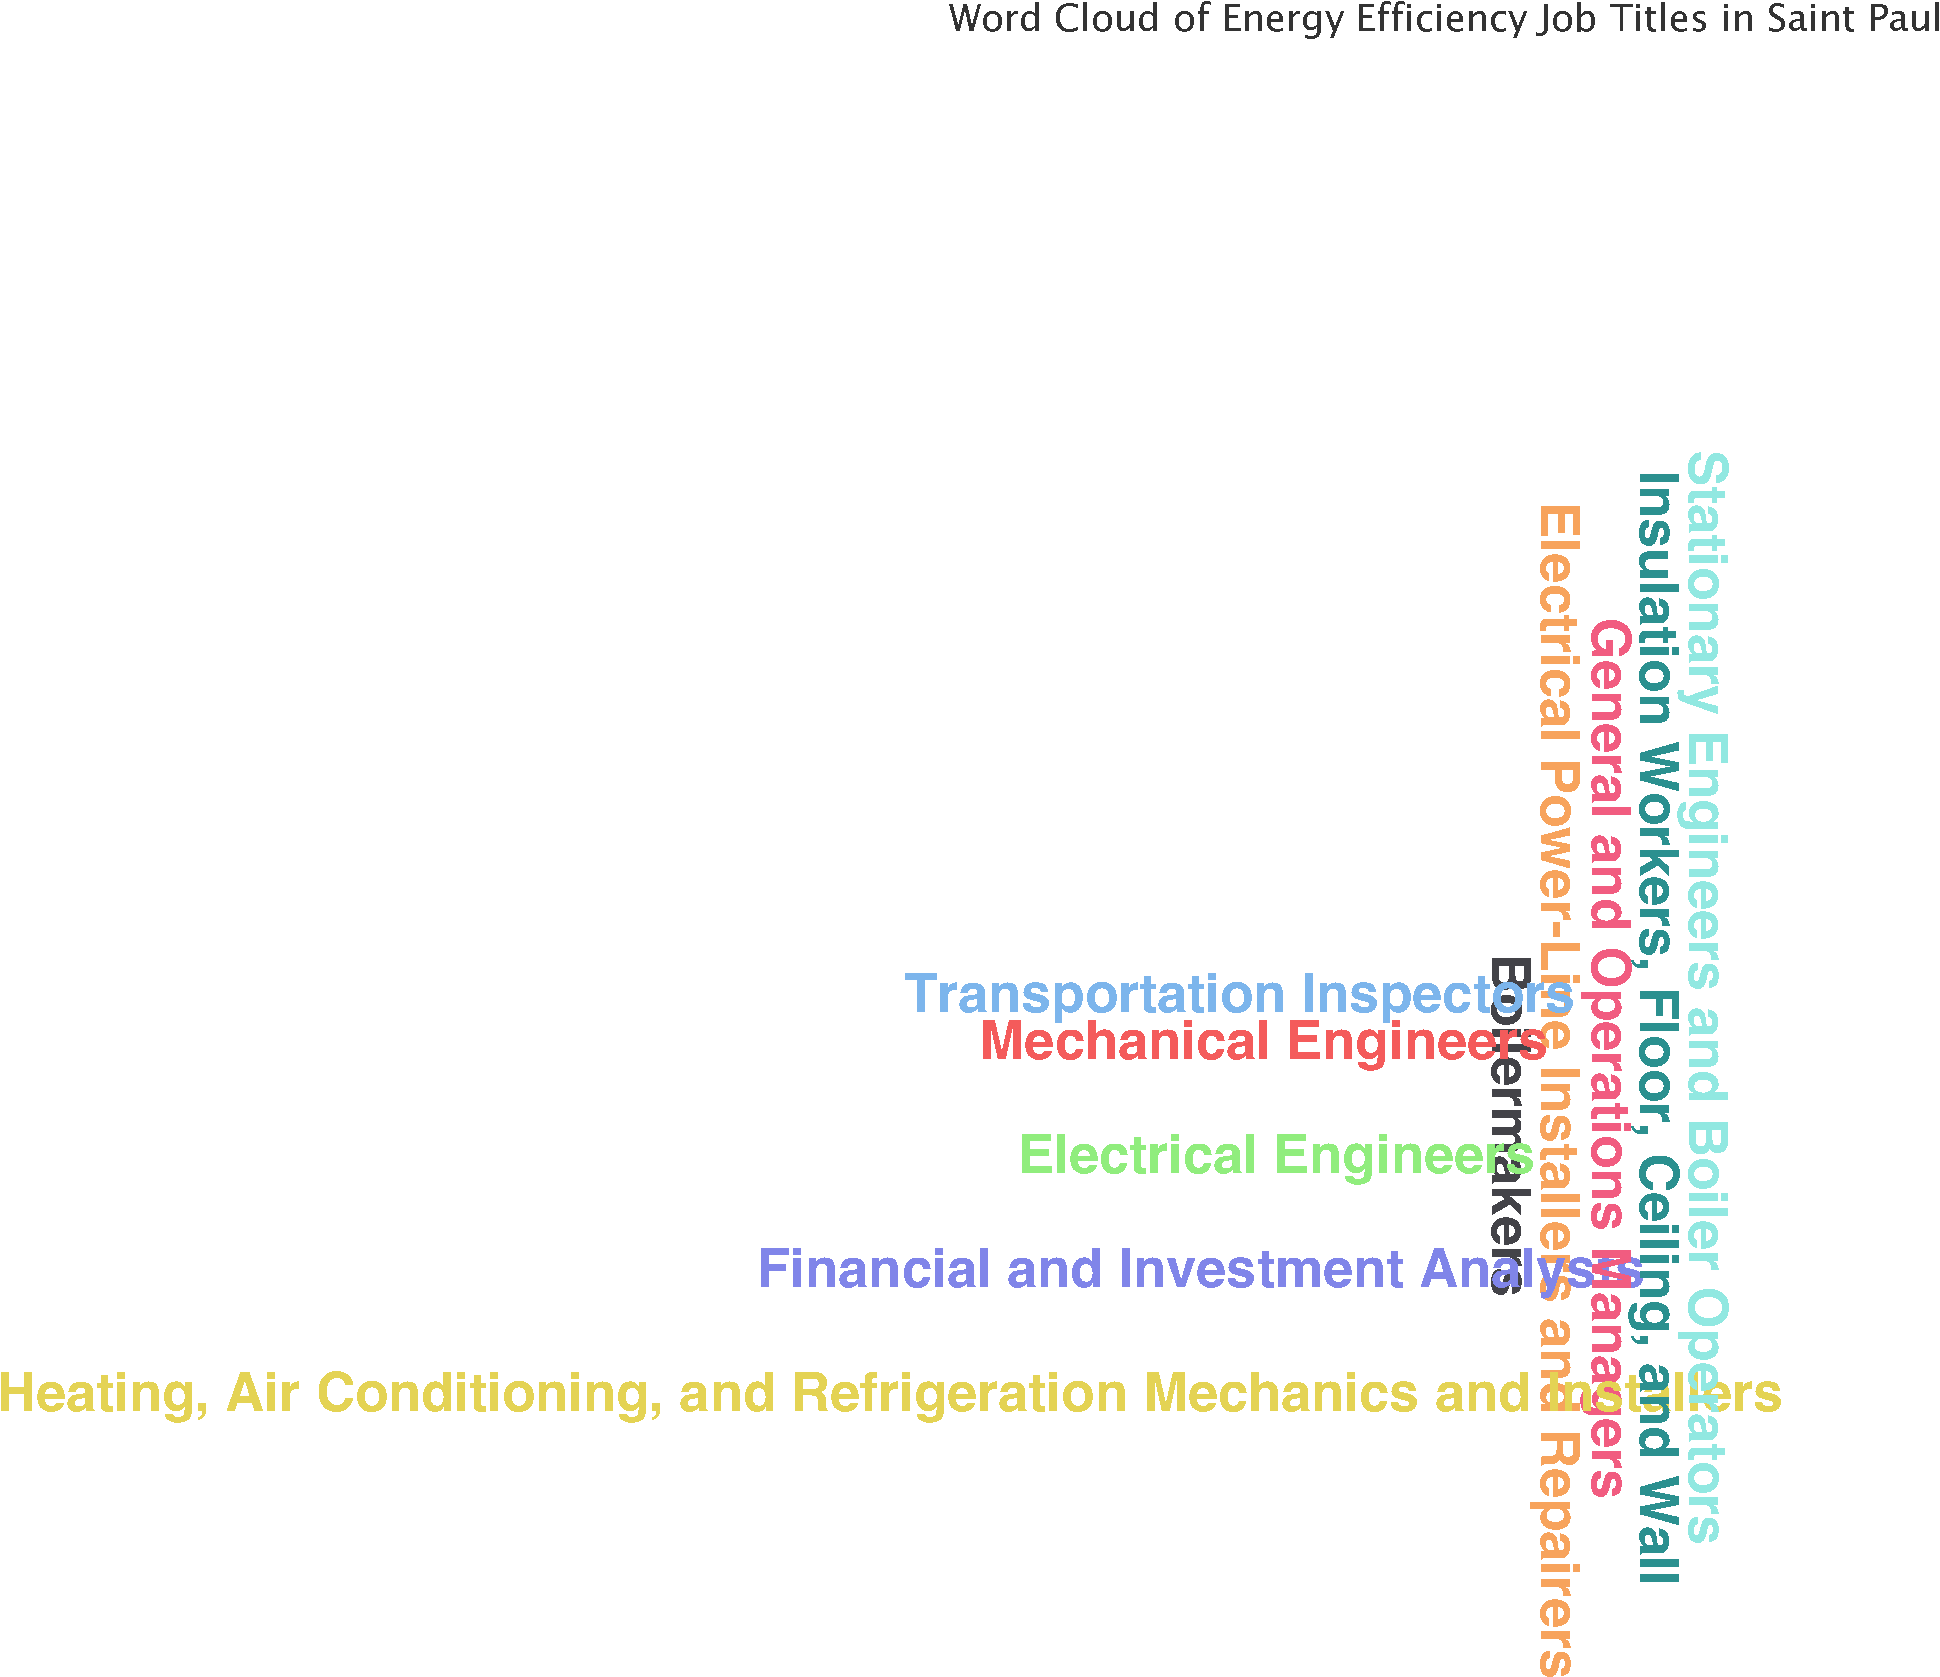
\includegraphics{index_files/figure-pdf/unnamed-chunk-23-1.pdf}

\begin{Shaded}
\begin{Highlighting}[]
\NormalTok{renewable\_energy\_wordcloud\_st\_paul}
\end{Highlighting}
\end{Shaded}

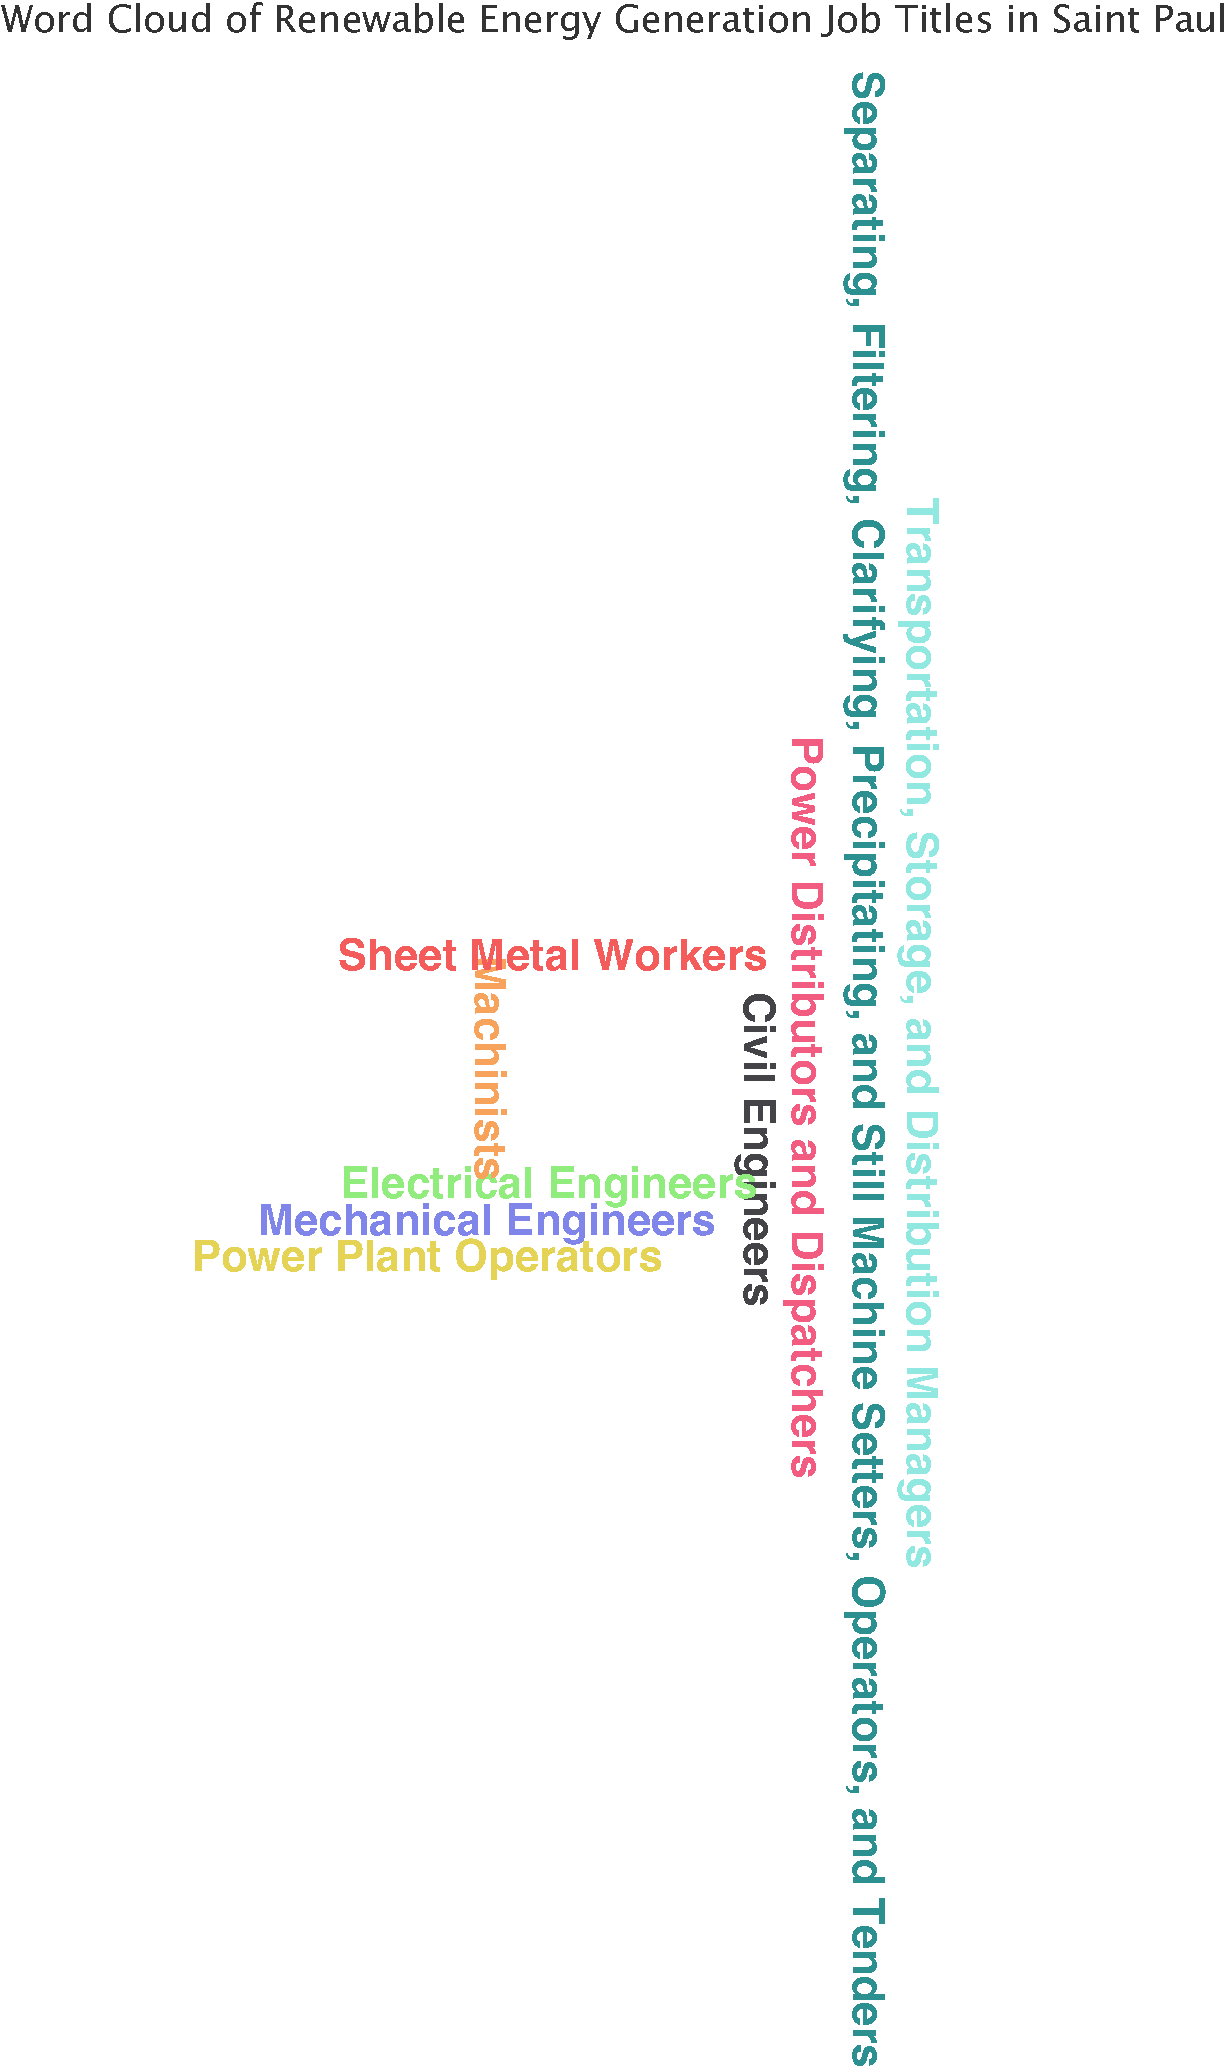
\includegraphics{index_files/figure-pdf/unnamed-chunk-23-2.pdf}

\begin{Shaded}
\begin{Highlighting}[]
\NormalTok{green\_construction\_wordcloud\_st\_paul}
\end{Highlighting}
\end{Shaded}

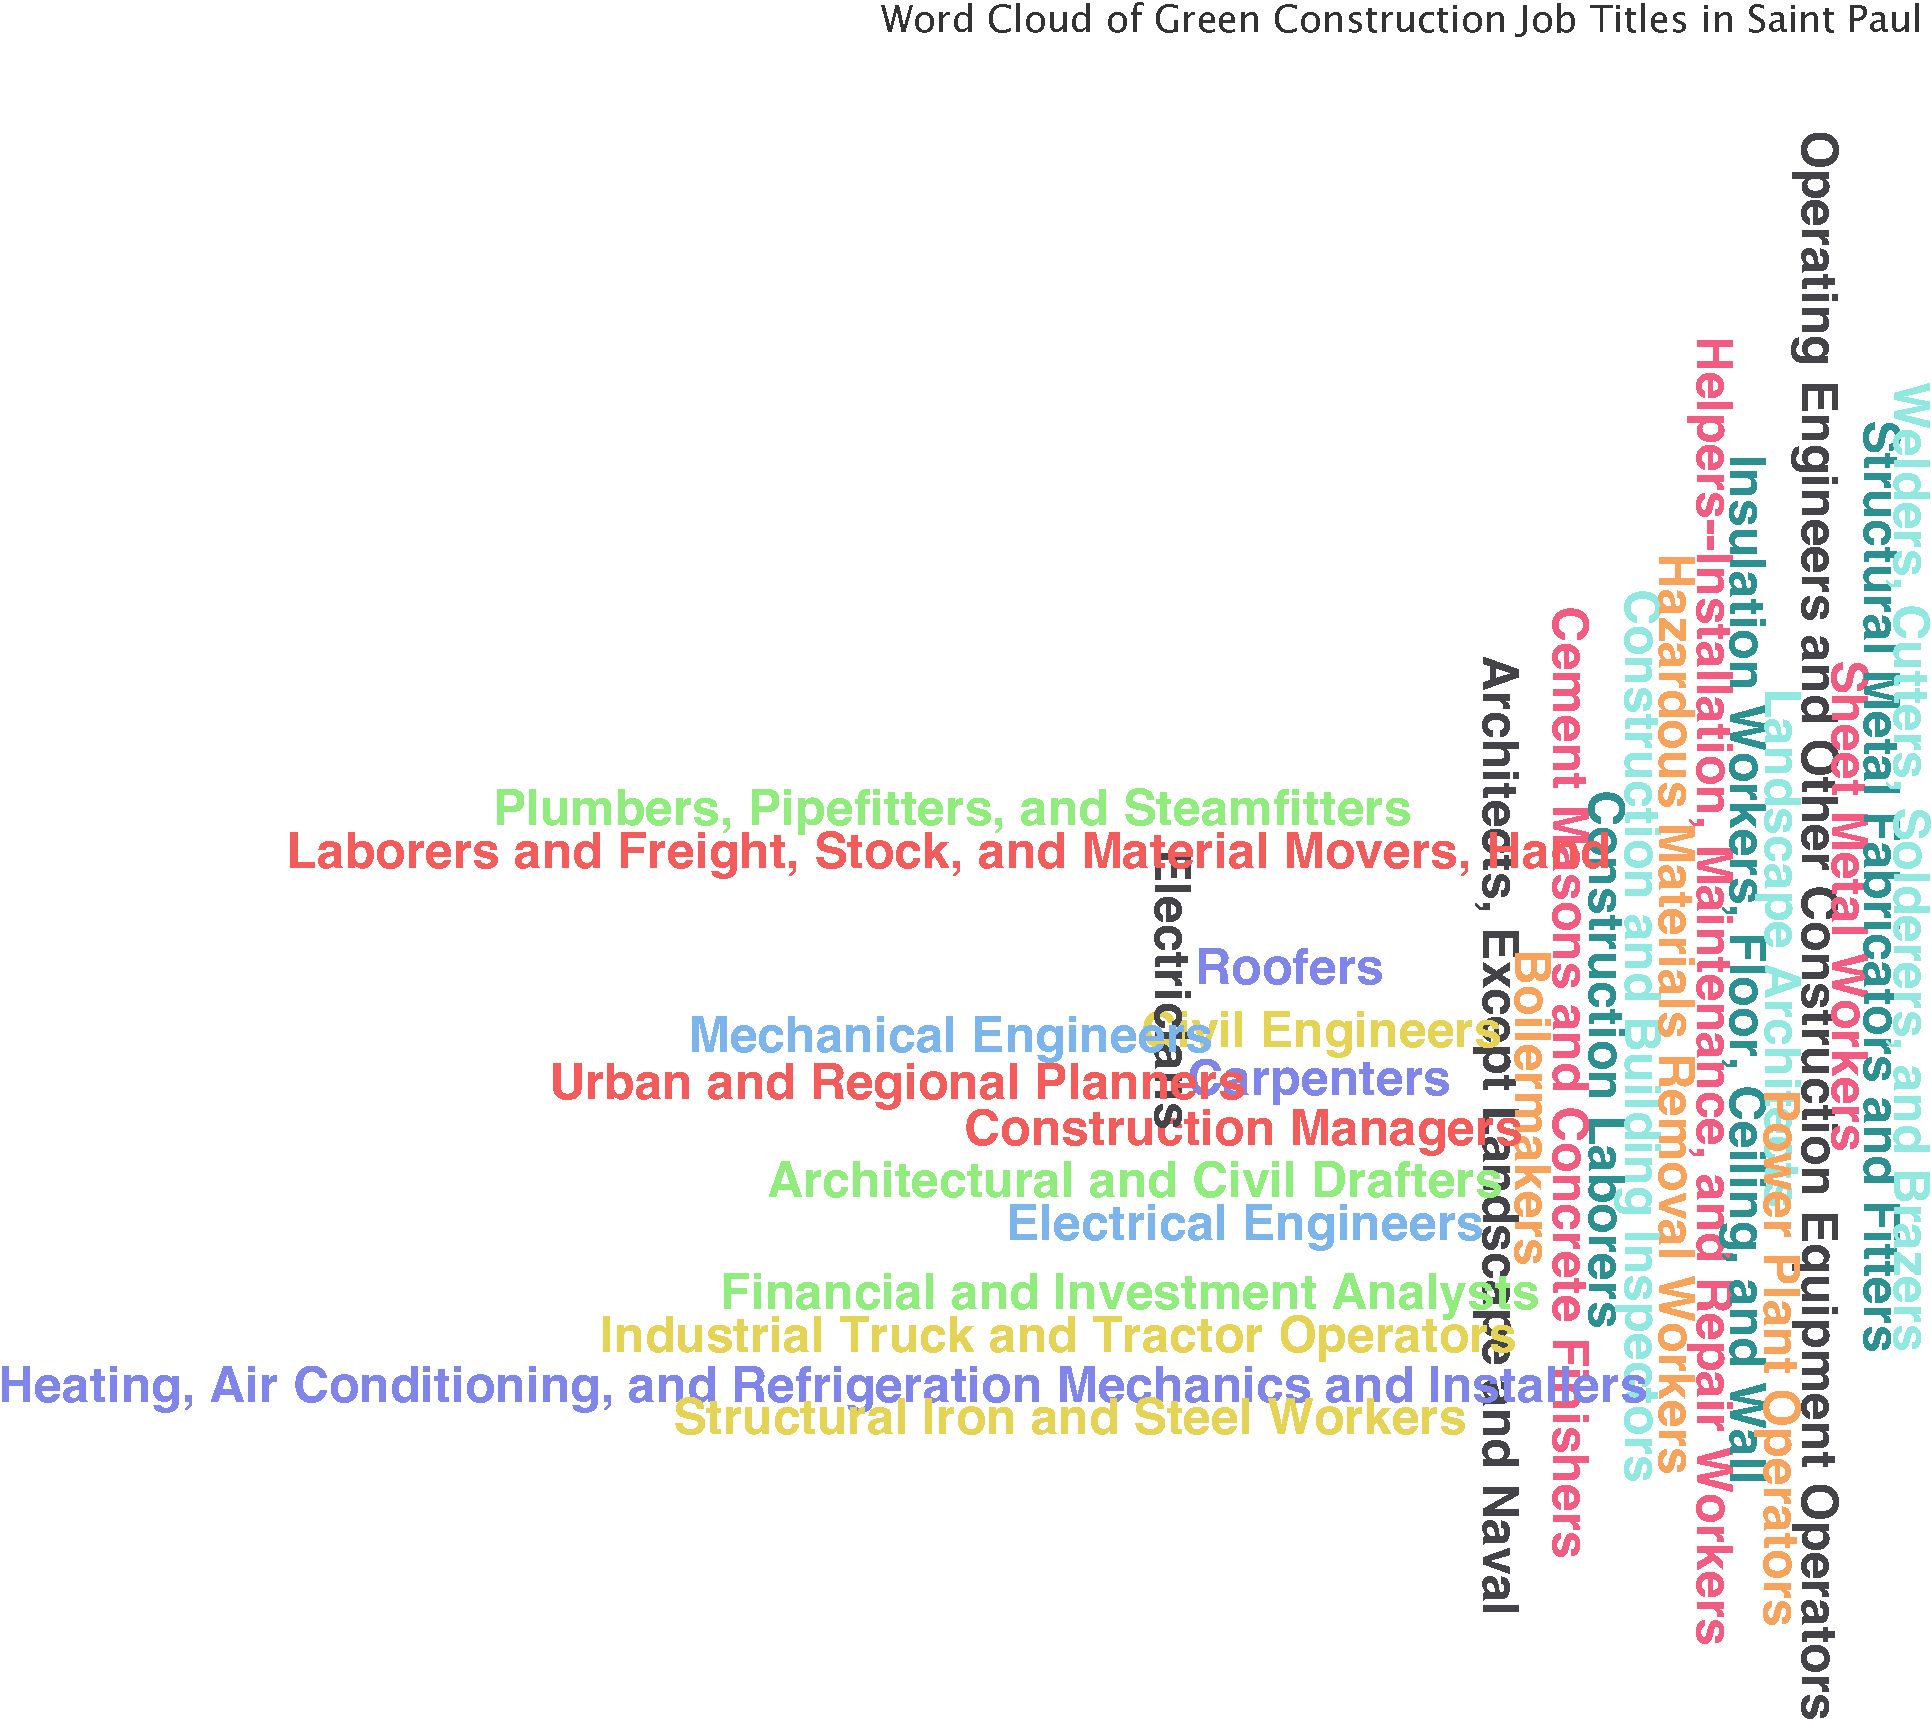
\includegraphics{index_files/figure-pdf/unnamed-chunk-23-3.pdf}

\textsubscript{Source:
\href{https://beeckcenter.github.io/climate-equity-workforce/index-preview.html}{Article
Notebook}}

Let's export for graphing

\begin{Shaded}
\begin{Highlighting}[]
\CommentTok{\# Export the St. Paul jobs data to CSV for graphing}
\FunctionTok{write.csv}\NormalTok{(st\_paul\_jobs, }\FunctionTok{here}\NormalTok{(}\StringTok{"processed\_data"}\NormalTok{, }\StringTok{"st\_paul\_jobs.csv"}\NormalTok{), }\AttributeTok{row.names =} \ConstantTok{FALSE}\NormalTok{)}

\CommentTok{\# Export the job\_type\_summary dataset for St. Paul to CSV for graphing}
\FunctionTok{write.csv}\NormalTok{(job\_type\_summary\_st\_paul, }\FunctionTok{here}\NormalTok{(}\StringTok{"processed\_data"}\NormalTok{, }\StringTok{"st\_paul\_job\_type\_summary.csv"}\NormalTok{), }\AttributeTok{row.names =} \ConstantTok{FALSE}\NormalTok{)}
\end{Highlighting}
\end{Shaded}

\textsubscript{Source:
\href{https://beeckcenter.github.io/climate-equity-workforce/index-preview.html}{Article
Notebook}}

\subsubsection{3. Quality, Pay, and Qualifications of Green
Jobs}\label{quality-pay-and-qualifications-of-green-jobs}

\begin{tcolorbox}[enhanced jigsaw, coltitle=black, opacitybacktitle=0.6, rightrule=.15mm, colframe=quarto-callout-note-color-frame, bottomtitle=1mm, title=\textcolor{quarto-callout-note-color}{\faInfo}\hspace{0.5em}{RQ 3: What is the quality of these green jobs? How much do they pay?
What qualifications are needed (education and experience) nationally?}, breakable, colback=white, toptitle=1mm, titlerule=0mm, arc=.35mm, opacityback=0, left=2mm, bottomrule=.15mm, toprule=.15mm, colbacktitle=quarto-callout-note-color!10!white, leftrule=.75mm]

\textbf{Higher education} is associated with better-quality green jobs,
particularly in the energy efficiency sector. Most high- and
medium-quality jobs in energy efficiency require at least a Bachelor's
Degree.

\textbf{Individuals with lower education levels} are more likely to end
up in green construction, especially in lower-quality jobs. Energy
efficiency tends to offer a better quality of jobs across all education
levels, with strong representation in both high and medium-quality
segments.

\textbf{Union membership} is \textbf{associated} with
\textbf{higher-quality jobs} in all three sectors, particularly in
energy efficiency and renewable energy generation, where a majority of
high-quality jobs are unionized.

\end{tcolorbox}

\begin{Shaded}
\begin{Highlighting}[]
\CommentTok{\# Import green job quality data}
\NormalTok{quality\_green\_jobs }\OtherTok{\textless{}{-}} \FunctionTok{read\_csv}\NormalTok{(}\FunctionTok{here}\NormalTok{(}\StringTok{"processed\_data"}\NormalTok{, }\StringTok{"Job\_Info\_Merged\_All\_Green.csv"}\NormalTok{))}
\end{Highlighting}
\end{Shaded}

\begin{verbatim}
Rows: 128 Columns: 29
-- Column specification --------------------------------------------------------
Delimiter: ","
chr (14): Reported Occupation, O*NET-SOC Code, O*NET-SOC Title, O*NET-SOC Ca...
dbl (15): Renewable Energy Generation, Energy Efficiency, Green Construction...

i Use `spec()` to retrieve the full column specification for this data.
i Specify the column types or set `show_col_types = FALSE` to quiet this message.
\end{verbatim}

\begin{Shaded}
\begin{Highlighting}[]
\FunctionTok{saveRDS}\NormalTok{(quality\_green\_jobs, }\FunctionTok{here}\NormalTok{(}\StringTok{"processed\_data"}\NormalTok{, }\StringTok{"quality\_green\_jobs.rds"}\NormalTok{))}

\NormalTok{quality\_green\_jobs }\OtherTok{\textless{}{-}} \FunctionTok{readRDS}\NormalTok{(}\FunctionTok{here}\NormalTok{(}\StringTok{"processed\_data"}\NormalTok{, }\StringTok{"quality\_green\_jobs.rds"}\NormalTok{))}
\end{Highlighting}
\end{Shaded}

\textsubscript{Source:
\href{https://beeckcenter.github.io/climate-equity-workforce/index-preview.html}{Article
Notebook}}

Now, let's transform this dataframe so it's visualization-ready.

\begin{Shaded}
\begin{Highlighting}[]
\CommentTok{\# Rename columns to snake\_case format}
\NormalTok{quality\_green\_jobs }\OtherTok{\textless{}{-}}\NormalTok{ quality\_green\_jobs }\SpecialCharTok{\%\textgreater{}\%}
  \FunctionTok{rename}\NormalTok{(}
    \AttributeTok{report\_occupation =} \StringTok{\textasciigrave{}}\AttributeTok{Reported Occupation}\StringTok{\textasciigrave{}}\NormalTok{,}
    \AttributeTok{onet\_soc\_code =} \StringTok{\textasciigrave{}}\AttributeTok{O*NET{-}SOC Code}\StringTok{\textasciigrave{}}\NormalTok{,}
    \AttributeTok{onet\_soc\_title =} \StringTok{\textasciigrave{}}\AttributeTok{O*NET{-}SOC Title}\StringTok{\textasciigrave{}}\NormalTok{,}
    \AttributeTok{onet\_soc\_category =} \StringTok{\textasciigrave{}}\AttributeTok{O*NET{-}SOC Category}\StringTok{\textasciigrave{}}\NormalTok{,}
    \AttributeTok{onet\_soc\_sector =} \StringTok{\textasciigrave{}}\AttributeTok{O*NET{-}SOC Sector}\StringTok{\textasciigrave{}}\NormalTok{,}
    \AttributeTok{renewable\_energy\_generation =} \StringTok{\textasciigrave{}}\AttributeTok{Renewable Energy Generation}\StringTok{\textasciigrave{}}\NormalTok{,}
    \AttributeTok{energy\_efficiency =} \StringTok{\textasciigrave{}}\AttributeTok{Energy Efficiency}\StringTok{\textasciigrave{}}\NormalTok{,}
    \AttributeTok{green\_construction =} \StringTok{\textasciigrave{}}\AttributeTok{Green Construction}\StringTok{\textasciigrave{}}\NormalTok{,}
    \AttributeTok{benchmark\_total =} \StringTok{\textasciigrave{}}\AttributeTok{Benchmark Total}\StringTok{\textasciigrave{}}\NormalTok{,}
    \AttributeTok{wage =}\NormalTok{ Wage,}
    \AttributeTok{forty\_hours =} \StringTok{\textasciigrave{}}\AttributeTok{40 hours}\StringTok{\textasciigrave{}}\NormalTok{,}
    \AttributeTok{schedule =}\NormalTok{ Schedule,}
    \AttributeTok{health\_ins =} \StringTok{\textasciigrave{}}\AttributeTok{Health Ins}\StringTok{\textasciigrave{}}\NormalTok{,}
    \AttributeTok{retirement =}\NormalTok{ Retirement,}
    \AttributeTok{growth =}\NormalTok{ Growth,}
    \AttributeTok{unemployment =}\NormalTok{ Unemployment,}
    \AttributeTok{illness\_injury =} \StringTok{\textasciigrave{}}\AttributeTok{Illness/injury}\StringTok{\textasciigrave{}}\NormalTok{,}
    \AttributeTok{ojt =}\NormalTok{ OJT,}
    \AttributeTok{union =}\NormalTok{ Union,}
    \AttributeTok{autonomy\_benchmark =}\NormalTok{ autonomy\_benchmark,}
    \AttributeTok{quality =}\NormalTok{ quality,}
    \AttributeTok{education =}\NormalTok{ education,}
    \AttributeTok{matrix\_title =} \StringTok{\textasciigrave{}}\AttributeTok{2022 National Employment Matrix title}\StringTok{\textasciigrave{}}\NormalTok{,}
    \AttributeTok{matrix\_code =} \StringTok{\textasciigrave{}}\AttributeTok{2022 National Employment Matrix code}\StringTok{\textasciigrave{}}\NormalTok{,}
    \AttributeTok{typical\_education\_needed =} \StringTok{\textasciigrave{}}\AttributeTok{Typical education needed for entry}\StringTok{\textasciigrave{}}\NormalTok{,}
    \AttributeTok{work\_experience\_related =} \StringTok{\textasciigrave{}}\AttributeTok{Work experience in a related occupation}\StringTok{\textasciigrave{}}\NormalTok{,}
    \AttributeTok{on\_the\_job\_training =} \StringTok{\textasciigrave{}}\AttributeTok{Typical on{-}the{-}job training needed to attain competency in the occupation}\StringTok{\textasciigrave{}}
\NormalTok{  )}
\end{Highlighting}
\end{Shaded}

\textsubscript{Source:
\href{https://beeckcenter.github.io/climate-equity-workforce/index-preview.html}{Article
Notebook}}

\begin{Shaded}
\begin{Highlighting}[]
\CommentTok{\# Convert the variables to the correct types}
\NormalTok{quality\_green\_jobs }\OtherTok{\textless{}{-}}\NormalTok{ quality\_green\_jobs }\SpecialCharTok{\%\textgreater{}\%}
  \FunctionTok{mutate}\NormalTok{(}
    \CommentTok{\# Factors}
    \AttributeTok{onet\_soc\_category =} \FunctionTok{factor}\NormalTok{(onet\_soc\_category),}
    \AttributeTok{onet\_soc\_sector =} \FunctionTok{factor}\NormalTok{(onet\_soc\_sector),}
    \AttributeTok{quality =} \FunctionTok{factor}\NormalTok{(quality, }\AttributeTok{levels =} \FunctionTok{c}\NormalTok{(}\StringTok{"Low Quality"}\NormalTok{, }\StringTok{"Medium Quality"}\NormalTok{, }\StringTok{"High Quality"}\NormalTok{)),}
    \AttributeTok{education =} \FunctionTok{factor}\NormalTok{(education),}
    \AttributeTok{typical\_education\_needed =} \FunctionTok{factor}\NormalTok{(typical\_education\_needed),}
    \AttributeTok{work\_experience\_related =} \FunctionTok{factor}\NormalTok{(work\_experience\_related),}
    \AttributeTok{on\_the\_job\_training =} \FunctionTok{factor}\NormalTok{(on\_the\_job\_training),}
    
    \CommentTok{\# Yes/No columns as numeric (1 for Yes, 0 for No)}
    \AttributeTok{renewable\_energy\_generation =} \FunctionTok{as.numeric}\NormalTok{(renewable\_energy\_generation),}
    \AttributeTok{energy\_efficiency =} \FunctionTok{as.numeric}\NormalTok{(energy\_efficiency),}
    \AttributeTok{green\_construction =} \FunctionTok{as.numeric}\NormalTok{(green\_construction),}
    \AttributeTok{wage =} \FunctionTok{as.numeric}\NormalTok{(wage),}
    \AttributeTok{forty\_hours =} \FunctionTok{as.numeric}\NormalTok{(forty\_hours),}
    \AttributeTok{schedule =} \FunctionTok{as.numeric}\NormalTok{(schedule),}
    \AttributeTok{health\_ins =} \FunctionTok{as.numeric}\NormalTok{(health\_ins),}
    \AttributeTok{retirement =} \FunctionTok{as.numeric}\NormalTok{(retirement),}
    \AttributeTok{growth =} \FunctionTok{as.numeric}\NormalTok{(growth),}
    \AttributeTok{unemployment =} \FunctionTok{as.numeric}\NormalTok{(unemployment),}
    \AttributeTok{illness\_injury =} \FunctionTok{as.numeric}\NormalTok{(illness\_injury),}
    \AttributeTok{ojt =} \FunctionTok{as.numeric}\NormalTok{(ojt),}
    \AttributeTok{union =} \FunctionTok{as.numeric}\NormalTok{(union),}
    \AttributeTok{autonomy\_benchmark =} \FunctionTok{as.numeric}\NormalTok{(autonomy\_benchmark)}
\NormalTok{  )}
\end{Highlighting}
\end{Shaded}

\textsubscript{Source:
\href{https://beeckcenter.github.io/climate-equity-workforce/index-preview.html}{Article
Notebook}}

\begin{Shaded}
\begin{Highlighting}[]
\CommentTok{\# Visualize quality jobs compared across sectors}
\NormalTok{quality\_summary }\OtherTok{\textless{}{-}}\NormalTok{ quality\_green\_jobs }\SpecialCharTok{\%\textgreater{}\%}
  \FunctionTok{gather}\NormalTok{(}\AttributeTok{key =} \StringTok{"sector"}\NormalTok{, }\AttributeTok{value =} \StringTok{"is\_green\_job"}\NormalTok{, renewable\_energy\_generation, energy\_efficiency, green\_construction) }\SpecialCharTok{\%\textgreater{}\%}
  \FunctionTok{filter}\NormalTok{(is\_green\_job }\SpecialCharTok{==} \DecValTok{1}\NormalTok{) }\SpecialCharTok{\%\textgreater{}\%}
  \FunctionTok{group\_by}\NormalTok{(sector, quality) }\SpecialCharTok{\%\textgreater{}\%}
  \FunctionTok{summarise}\NormalTok{(}\AttributeTok{count =} \FunctionTok{n}\NormalTok{()) }\SpecialCharTok{\%\textgreater{}\%}
  \FunctionTok{mutate}\NormalTok{(}\AttributeTok{percentage =}\NormalTok{ count }\SpecialCharTok{/} \FunctionTok{sum}\NormalTok{(count) }\SpecialCharTok{*} \DecValTok{100}\NormalTok{)}
\end{Highlighting}
\end{Shaded}

\begin{verbatim}
`summarise()` has grouped output by 'sector'. You can override using the
`.groups` argument.
\end{verbatim}

\begin{Shaded}
\begin{Highlighting}[]
\FunctionTok{ggplot}\NormalTok{(quality\_summary, }\FunctionTok{aes}\NormalTok{(}\AttributeTok{x =}\NormalTok{ sector, }\AttributeTok{y =}\NormalTok{ percentage, }\AttributeTok{fill =}\NormalTok{ quality)) }\SpecialCharTok{+}
  \FunctionTok{geom\_bar}\NormalTok{(}\AttributeTok{stat =} \StringTok{"identity"}\NormalTok{, }\AttributeTok{position =} \StringTok{"fill"}\NormalTok{, }\AttributeTok{width =} \FloatTok{0.7}\NormalTok{) }\SpecialCharTok{+}
  \FunctionTok{geom\_text}\NormalTok{(}\FunctionTok{aes}\NormalTok{(}\AttributeTok{label =} \FunctionTok{paste0}\NormalTok{(}\FunctionTok{round}\NormalTok{(percentage, }\DecValTok{1}\NormalTok{), }\StringTok{"\%"}\NormalTok{)), }
            \AttributeTok{position =} \FunctionTok{position\_fill}\NormalTok{(}\AttributeTok{vjust =} \FloatTok{0.5}\NormalTok{), }\AttributeTok{size =} \DecValTok{4}\NormalTok{) }\SpecialCharTok{+}
  \FunctionTok{labs}\NormalTok{(}\AttributeTok{x =} \StringTok{"Sector"}\NormalTok{, }\AttributeTok{y =} \StringTok{"Percentage"}\NormalTok{, }\AttributeTok{title =} \StringTok{"Green Job Quality by Sector"}\NormalTok{) }\SpecialCharTok{+}
  \FunctionTok{scale\_fill\_manual}\NormalTok{(}\AttributeTok{values =} \FunctionTok{c}\NormalTok{(}\StringTok{"High Quality"} \OtherTok{=} \StringTok{"\#1f77b4"}\NormalTok{, }\StringTok{"Medium Quality"} \OtherTok{=} \StringTok{"\#ffbb78"}\NormalTok{, }\StringTok{"Low Quality"} \OtherTok{=} \StringTok{"\#2ca02c"}\NormalTok{)) }\SpecialCharTok{+}
  \FunctionTok{theme\_minimal}\NormalTok{() }\SpecialCharTok{+}
  \FunctionTok{theme}\NormalTok{(}\AttributeTok{legend.title =} \FunctionTok{element\_blank}\NormalTok{())}
\end{Highlighting}
\end{Shaded}

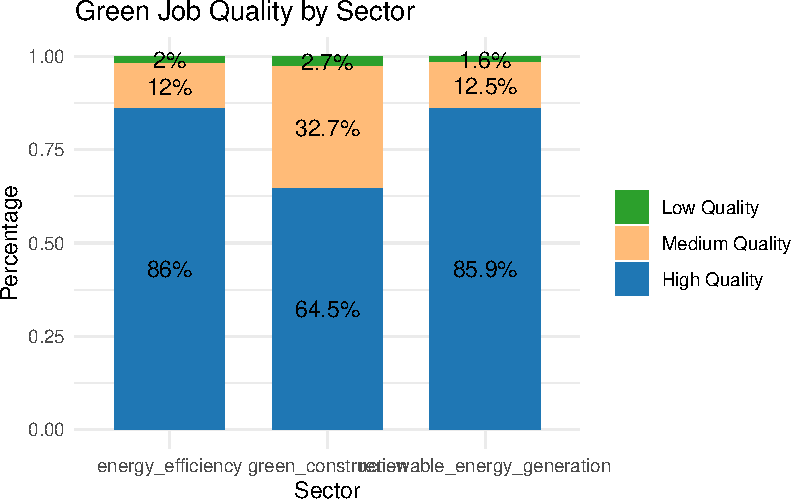
\includegraphics{index_files/figure-pdf/unnamed-chunk-28-1.pdf}

\textsubscript{Source:
\href{https://beeckcenter.github.io/climate-equity-workforce/index-preview.html}{Article
Notebook}}

\begin{Shaded}
\begin{Highlighting}[]
\CommentTok{\# Visualize quality jobs compared for sector, education, and quality}
\NormalTok{quality\_summary\_education }\OtherTok{\textless{}{-}}\NormalTok{ quality\_green\_jobs }\SpecialCharTok{\%\textgreater{}\%}
  \FunctionTok{gather}\NormalTok{(}\AttributeTok{key =} \StringTok{"sector"}\NormalTok{, }\AttributeTok{value =} \StringTok{"is\_green\_job"}\NormalTok{, renewable\_energy\_generation, energy\_efficiency, green\_construction) }\SpecialCharTok{\%\textgreater{}\%}
  \FunctionTok{filter}\NormalTok{(is\_green\_job }\SpecialCharTok{==} \DecValTok{1}\NormalTok{) }\SpecialCharTok{\%\textgreater{}\%}
  \FunctionTok{group\_by}\NormalTok{(sector, quality, education) }\SpecialCharTok{\%\textgreater{}\%}
  \FunctionTok{summarise}\NormalTok{(}\AttributeTok{count =} \FunctionTok{n}\NormalTok{()) }\SpecialCharTok{\%\textgreater{}\%}
  \FunctionTok{mutate}\NormalTok{(}\AttributeTok{percentage =}\NormalTok{ count }\SpecialCharTok{/} \FunctionTok{sum}\NormalTok{(count) }\SpecialCharTok{*} \DecValTok{100}\NormalTok{)}
\end{Highlighting}
\end{Shaded}

\begin{verbatim}
`summarise()` has grouped output by 'sector', 'quality'. You can override using
the `.groups` argument.
\end{verbatim}

\begin{Shaded}
\begin{Highlighting}[]
\FunctionTok{ggplot}\NormalTok{(quality\_summary\_education, }\FunctionTok{aes}\NormalTok{(}\AttributeTok{x =}\NormalTok{ education, }\AttributeTok{y =}\NormalTok{ percentage, }\AttributeTok{fill =}\NormalTok{ sector)) }\SpecialCharTok{+}
  \FunctionTok{geom\_bar}\NormalTok{(}\AttributeTok{stat =} \StringTok{"identity"}\NormalTok{, }\AttributeTok{position =} \StringTok{"dodge"}\NormalTok{) }\SpecialCharTok{+}
  \FunctionTok{facet\_wrap}\NormalTok{(}\SpecialCharTok{\textasciitilde{}}\NormalTok{ quality, }\AttributeTok{ncol =} \DecValTok{1}\NormalTok{, }\AttributeTok{scales =} \StringTok{"free\_y"}\NormalTok{) }\SpecialCharTok{+} \CommentTok{\# Separate the quality levels}
  \FunctionTok{geom\_text}\NormalTok{(}\FunctionTok{aes}\NormalTok{(}\AttributeTok{label =} \FunctionTok{paste0}\NormalTok{(}\FunctionTok{round}\NormalTok{(percentage, }\DecValTok{1}\NormalTok{), }\StringTok{"\%"}\NormalTok{)), }
            \AttributeTok{position =} \FunctionTok{position\_dodge}\NormalTok{(}\AttributeTok{width =} \FloatTok{0.9}\NormalTok{), }\AttributeTok{vjust =} \SpecialCharTok{{-}}\FloatTok{0.5}\NormalTok{, }\AttributeTok{size =} \DecValTok{3}\NormalTok{) }\SpecialCharTok{+}
  \FunctionTok{labs}\NormalTok{(}\AttributeTok{x =} \StringTok{"Education Level"}\NormalTok{, }\AttributeTok{y =} \StringTok{"Percentage"}\NormalTok{, }\AttributeTok{title =} \StringTok{"Green Job Quality by Sector and Education"}\NormalTok{) }\SpecialCharTok{+}
  \FunctionTok{theme\_minimal}\NormalTok{() }\SpecialCharTok{+}
  \FunctionTok{theme}\NormalTok{(}\AttributeTok{legend.title =} \FunctionTok{element\_blank}\NormalTok{(), }\AttributeTok{axis.text.x =} \FunctionTok{element\_text}\NormalTok{(}\AttributeTok{angle =} \DecValTok{45}\NormalTok{, }\AttributeTok{hjust =} \DecValTok{1}\NormalTok{))}
\end{Highlighting}
\end{Shaded}

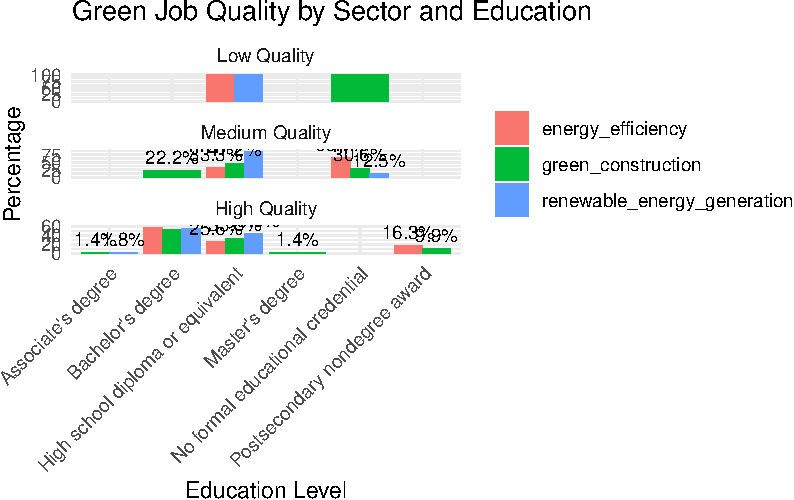
\includegraphics{index_files/figure-pdf/unnamed-chunk-29-1.pdf}

\textsubscript{Source:
\href{https://beeckcenter.github.io/climate-equity-workforce/index-preview.html}{Article
Notebook}}

This graph shows how the distribution of green jobs (energy efficiency,
green construction, renewable energy generation) varies across different
levels of education, segmented by job quality (Low, Medium, High
quality).

Based on the above graph:

\begin{itemize}
\item
  \textbf{Energy Efficiency} consistently dominates high-quality and
  medium-quality green jobs across most education levels, suggesting
  that this sector offers the most secure and rewarding jobs for those
  with varying levels of education.
\item
  \textbf{Green Construction} has a significant presence in low-quality
  and medium-quality jobs, especially for those with lower education
  levels (such as high school diplomas or no formal educational
  credentials).
\item
  \textbf{Renewable Energy Generation} seems to have fewer high-quality
  job opportunities compared to energy efficiency, but it does offer
  medium-quality opportunities, particularly for those with lower
  education levels.
\end{itemize}

\begin{Shaded}
\begin{Highlighting}[]
\CommentTok{\# \# Matrix table that shows green job quality segmented by variables from wage to union across the three sectors (renewable\_energy\_generation, energy\_efficiency, green\_construction)}

\CommentTok{\# \# Transform the data to long format}
\CommentTok{\# long\_quality\_jobs \textless{}{-} quality\_green\_jobs \%\textgreater{}\%}
\CommentTok{\#   gather(key = "sector", value = "is\_green\_job", renewable\_energy\_generation, energy\_efficiency, green\_construction) \%\textgreater{}\%}
\CommentTok{\#   filter(is\_green\_job == 1) \%\textgreater{}\%}
\CommentTok{\#   select(sector, quality, wage, forty\_hours, schedule, health\_ins, retirement, growth, unemployment, illness\_injury, ojt, union, autonomy\_benchmark) \%\textgreater{}\%}
\CommentTok{\#   pivot\_longer(cols = wage:autonomy\_benchmark, names\_to = "variable", values\_to = "value") \%\textgreater{}\%}
\CommentTok{\#   group\_by(sector, quality, variable) \%\textgreater{}\%}
\CommentTok{\#   summarise(proportion = mean(value)) \%\textgreater{}\%}
\CommentTok{\#   ungroup() \%\textgreater{}\%}
\CommentTok{\#   arrange(sector, quality, variable)}
\CommentTok{\# }
\CommentTok{\# \# Generate matrix table using gt}
\CommentTok{\# matrix\_table \textless{}{-} long\_quality\_jobs \%\textgreater{}\%}
\CommentTok{\#   pivot\_wider(names\_from = quality, values\_from = proportion) \%\textgreater{}\%}
\CommentTok{\#   gt() \%\textgreater{}\%}
\CommentTok{\#   tab\_header(}
\CommentTok{\#     title = "Green Job Quality Matrix by Sector and Variables",}
\CommentTok{\#     subtitle = "Proportion of Each Job Quality Level Across Wage, Hours, Benefits, etc."}
\CommentTok{\#   ) \%\textgreater{}\%}
\CommentTok{\#   fmt\_number(}
\CommentTok{\#     columns = vars(\textasciigrave{}High Quality\textasciigrave{}, \textasciigrave{}Medium Quality\textasciigrave{}, \textasciigrave{}Low Quality\textasciigrave{}),}
\CommentTok{\#     decimals = 2}
\CommentTok{\#   )}
\CommentTok{\# }
\CommentTok{\# \# Display the matrix table}
\CommentTok{\# print(matrix\_table)}
\end{Highlighting}
\end{Shaded}

\textsubscript{Source:
\href{https://beeckcenter.github.io/climate-equity-workforce/index-preview.html}{Article
Notebook}}

\begin{Shaded}
\begin{Highlighting}[]
\CommentTok{\# Visualize quality jobs compared for sector, union membership, and quality}
\NormalTok{quality\_summary\_union }\OtherTok{\textless{}{-}}\NormalTok{ quality\_green\_jobs }\SpecialCharTok{\%\textgreater{}\%}
  \FunctionTok{gather}\NormalTok{(}\AttributeTok{key =} \StringTok{"sector"}\NormalTok{, }\AttributeTok{value =} \StringTok{"is\_green\_job"}\NormalTok{, renewable\_energy\_generation, energy\_efficiency, green\_construction) }\SpecialCharTok{\%\textgreater{}\%}
  \FunctionTok{filter}\NormalTok{(is\_green\_job }\SpecialCharTok{==} \DecValTok{1}\NormalTok{) }\SpecialCharTok{\%\textgreater{}\%}
  \FunctionTok{group\_by}\NormalTok{(sector, quality, union) }\SpecialCharTok{\%\textgreater{}\%}
  \FunctionTok{summarise}\NormalTok{(}\AttributeTok{count =} \FunctionTok{n}\NormalTok{()) }\SpecialCharTok{\%\textgreater{}\%}
  \FunctionTok{mutate}\NormalTok{(}\AttributeTok{percentage =}\NormalTok{ count }\SpecialCharTok{/} \FunctionTok{sum}\NormalTok{(count) }\SpecialCharTok{*} \DecValTok{100}\NormalTok{)}
\end{Highlighting}
\end{Shaded}

\begin{verbatim}
`summarise()` has grouped output by 'sector', 'quality'. You can override using
the `.groups` argument.
\end{verbatim}

\begin{Shaded}
\begin{Highlighting}[]
\FunctionTok{ggplot}\NormalTok{(quality\_summary\_union, }\FunctionTok{aes}\NormalTok{(}\AttributeTok{x =} \FunctionTok{as.factor}\NormalTok{(union), }\AttributeTok{y =}\NormalTok{ percentage, }\AttributeTok{fill =}\NormalTok{ sector)) }\SpecialCharTok{+}
  \FunctionTok{geom\_bar}\NormalTok{(}\AttributeTok{stat =} \StringTok{"identity"}\NormalTok{, }\AttributeTok{position =} \StringTok{"dodge"}\NormalTok{) }\SpecialCharTok{+}
  \FunctionTok{facet\_wrap}\NormalTok{(}\SpecialCharTok{\textasciitilde{}}\NormalTok{ quality, }\AttributeTok{ncol =} \DecValTok{1}\NormalTok{, }\AttributeTok{scales =} \StringTok{"free\_y"}\NormalTok{) }\SpecialCharTok{+} \CommentTok{\# Separate the quality levels}
  \FunctionTok{geom\_text}\NormalTok{(}\FunctionTok{aes}\NormalTok{(}\AttributeTok{label =} \FunctionTok{paste0}\NormalTok{(}\FunctionTok{round}\NormalTok{(percentage, }\DecValTok{1}\NormalTok{), }\StringTok{"\%"}\NormalTok{)), }
            \AttributeTok{position =} \FunctionTok{position\_dodge}\NormalTok{(}\AttributeTok{width =} \FloatTok{0.9}\NormalTok{), }\AttributeTok{vjust =} \SpecialCharTok{{-}}\FloatTok{0.5}\NormalTok{, }\AttributeTok{size =} \DecValTok{3}\NormalTok{) }\SpecialCharTok{+}
  \FunctionTok{labs}\NormalTok{(}\AttributeTok{x =} \StringTok{"Union Membership"}\NormalTok{, }\AttributeTok{y =} \StringTok{"Percentage"}\NormalTok{, }\AttributeTok{title =} \StringTok{"Green Job Quality by Sector and Union Membership"}\NormalTok{) }\SpecialCharTok{+}
  \FunctionTok{theme\_minimal}\NormalTok{() }\SpecialCharTok{+}
  \FunctionTok{theme}\NormalTok{(}\AttributeTok{legend.title =} \FunctionTok{element\_blank}\NormalTok{(), }\AttributeTok{axis.text.x =} \FunctionTok{element\_text}\NormalTok{(}\AttributeTok{angle =} \DecValTok{45}\NormalTok{, }\AttributeTok{hjust =} \DecValTok{1}\NormalTok{))}
\end{Highlighting}
\end{Shaded}

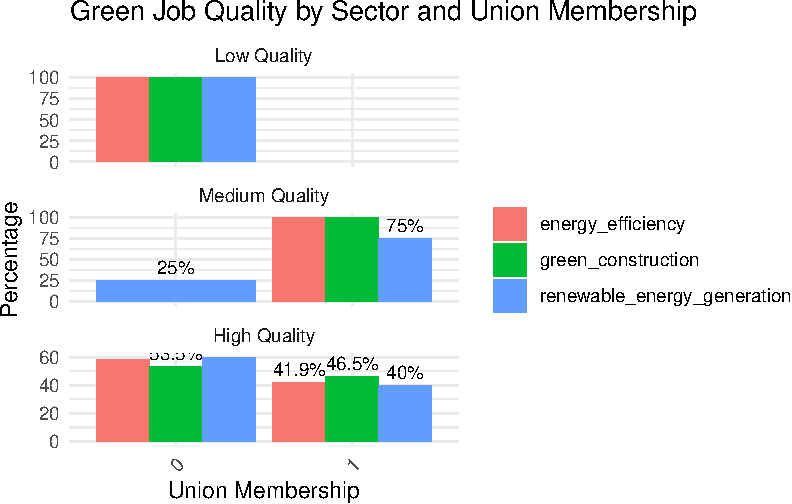
\includegraphics{index_files/figure-pdf/unnamed-chunk-31-1.pdf}

\textsubscript{Source:
\href{https://beeckcenter.github.io/climate-equity-workforce/index-preview.html}{Article
Notebook}}

The above graph shows green job quality segmented by union membership
across three sectors: \textbf{Energy Efficiency}, \textbf{Green
Construction}, and \textbf{Renewable Energy Generation}.

\begin{itemize}
\item
  \textbf{Union membership} is \textbf{associated} with
  \textbf{higher-quality jobs} in all three sectors, particularly in
  energy efficiency and renewable energy generation, where a majority of
  high-quality jobs are unionized. This suggests that \textbf{unions
  play a significant role in securing better working conditions and
  benefits} for workers in green jobs.
\item
  \textbf{Medium-quality jobs} also show a clear advantage for unionized
  workers across the sectors, particularly in green construction and
  renewable energy generation.
\item
  The presence of \textbf{union coverage even in low-quality jobs}
  across sectors might indicate that unionized jobs are spread across
  different quality categories, though the majority of benefits seem to
  concentrate in medium- and high-quality roles.
\end{itemize}

\begin{Shaded}
\begin{Highlighting}[]
\CommentTok{\# Export the green quality jobs data to CSV for graphing}
\FunctionTok{saveRDS}\NormalTok{(quality\_green\_jobs, }\FunctionTok{here}\NormalTok{(}\StringTok{"processed\_data"}\NormalTok{, }\StringTok{"quality\_green\_jobs.rds"}\NormalTok{))}

\FunctionTok{write\_csv}\NormalTok{(quality\_green\_jobs, }\FunctionTok{here}\NormalTok{(}\StringTok{"processed\_data"}\NormalTok{, }\StringTok{"quality\_green\_jobs.csv"}\NormalTok{))}
\end{Highlighting}
\end{Shaded}

\textsubscript{Source:
\href{https://beeckcenter.github.io/climate-equity-workforce/index-preview.html}{Article
Notebook}}

\subsubsection{4. Demographics of Green Job
Recipients}\label{demographics-of-green-job-recipients}

\begin{tcolorbox}[enhanced jigsaw, coltitle=black, opacitybacktitle=0.6, rightrule=.15mm, colframe=quarto-callout-note-color-frame, bottomtitle=1mm, title=\textcolor{quarto-callout-note-color}{\faInfo}\hspace{0.5em}{RQ 4: Who is getting these green jobs, based on education,
race/ethnicity, gender, and income levels in the City of Saint Paul?}, breakable, colback=white, toptitle=1mm, titlerule=0mm, arc=.35mm, opacityback=0, left=2mm, bottomrule=.15mm, toprule=.15mm, colbacktitle=quarto-callout-note-color!10!white, leftrule=.75mm]

Of the more than \textbf{303,820 people} who live in \textbf{St.~Paul},
\textbf{50.5\%} are women, which is aligned with the national average.
The majority of residents in St.~Paul are \textbf{white} (54.3\%).
\textbf{Black or African American people} (15.6\%) make up the largest
community of color in the city. Other \textbf{communities of color,}
including Asian (18.4\%), Alaska and Native American (0.7\%), Hispanic
or Latino (8.6\%) and Two or More Races (7.8\%), make up about 41.5\% of
the population. Around \textbf{42.8\% of people aged 25 and older have a
bachelor's degree} in St.~Paul, which is higher than the national rate
of 34\% but lower than Minneapolis' 54\%.

\end{tcolorbox}

In the following figures, we describe the challenges women and people of
color in Saint Paul are likely to face in equitably accessing the jobs
that may be created through BIL and IRA funding in three specific
sectors: energy efficiency, renewable-energy generation, and green
construction.

\begin{itemize}
\item
  \textbf{2023 Occupational Employment and Wage Survey (OEWS):}

  \begin{itemize}
  \item
    Provides employment and wage data by occupation.
  \item
    It's organized at the \textbf{Metropolitan Statistical Area (MSA)}
    level, which includes a broader geographic area (e.g.,
    Minneapolis-St.~Paul-Bloomington, MN-WI Metro).
  \item
    This data gives insights into \textbf{jobs and wages} but lacks
    detailed individual demographics such as race, ethnicity, education,
    etc.
  \end{itemize}
\item
  \textbf{Geocorr Data from the Missouri Census Data Center:}

  \begin{itemize}
  \item
    This data helps map geographic boundaries like PUMAs (Public Use
    Microdata Areas) to more specific local areas, such as St.~Paul.
  \item
    By using geographic weighting from Geocorr, we can estimate
    \textbf{St.~Paul-specific} statistics from the broader MSA-level
    data in the OEWS.
  \end{itemize}
\end{itemize}

\begin{enumerate}
\def\labelenumi{\arabic{enumi}.}
\tightlist
\item
  Load and explore the two datasets.
\item
  Filter the OEWS data to the Minneapolis-St.~Paul-Bloomington Metro
  area.
\item
  Get weights from the Geocorr file to adjust for St.~Paul's population.
\item
  Merge demographic data (from ACS) with the estimated job/wage data
  from OEWS.
\item
  Analyze the final dataset for insights into who holds green jobs in
  St.~Paul.
\end{enumerate}

\textbf{2023 Occupational Employment and Wage Survey}

✅\href{https://docs.google.com/spreadsheets/d/1I2munGunOJgdI2iWRW7p0BVU0O13r4zb/edit?gid=1944656488\#gid=1944656488}{National
level data}

✅\href{https://docs.google.com/spreadsheets/d/105RYiRn-1LIVC-iUdCD3fCKROfOGH_M62s45gbo7GFM/edit?gid=2141627594\#gid=2141627594}{Minneapolis-St.~Paul-Bloomington,
MN-WI}

\textbf{Geocorr from the Missouri Census Data Center}

\href{https://docs.google.com/spreadsheets/d/1wRr-jATTjaXpErUfSCAZsoSn-lt1-TZtWv_Hoq2C29Q/edit?gid=1877088889\#gid=1877088889}{Minnesota
Level~}: Contains data mapping PUMAs to Metropolitan Statistical Areas
and PUMAs to cities

\textbf{Processed}~

\href{https://drive.google.com/file/d/1uyRoXlExkExjlJytEh8meqD3D--4Hwj4/view?usp=drive_link}{St.~Paul
- ACS PUMS - Five Years + O*NET Green Jobs}

\href{https://drive.google.com/file/d/1C3opSLifg144MIYnISHmf7wwZuAe2TQJ/view?usp=drive_link}{National
- ACS PUMS - Five Years + O*NET Green Jobs}

We will first need to load the \textbf{OEWS} data (Occupational
Employment and Wage Survey) and the \textbf{Geocorr} data (geographic
weights from the Missouri Census Data Center) into R.

\begin{itemize}
\item
  \textbf{OEWS:} processed\_data/OWES\_and\_ONET\_St\_Paul
\item
  \textbf{Geocorr:} raw\_data/Geocorr from the Missouri Census Data
  Center - Minnesota.xlsx
\end{itemize}

We have the \textbf{ACS (American Community Survey)} data that provides
demographic information (education, race, gender, income), so we'll load
that as well.

\begin{itemize}
\tightlist
\item
  \textbf{ACS:} processed\_data/St\_Paul\_ACS\_All\_Jobs.csv
\end{itemize}

\textbf{Load the OEWS data} (Occupational Employment and Wage Survey),
the Geocorr data (geographic weights from the Missouri Census Data
Center), and the ACS (American Community Survey) data that provides
demographic information (education, race, gender, income). The OEWS
Data: is already filtered to the Minneapolis-St.~Paul-Bloomington, MN-WI
Metro Area.

\begin{Shaded}
\begin{Highlighting}[]
\CommentTok{\# Load St. Paul jobs data (OEWS dataset)}
\NormalTok{st\_paul\_jobs }\OtherTok{\textless{}{-}} \FunctionTok{read\_csv}\NormalTok{(}\FunctionTok{here}\NormalTok{(}\StringTok{"processed\_data"}\NormalTok{, }\StringTok{"OWES\_and\_ONET{-}St\_Paul.csv"}\NormalTok{))}
\end{Highlighting}
\end{Shaded}

\begin{verbatim}
Rows: 742 Columns: 34
-- Column specification --------------------------------------------------------
Delimiter: ","
chr (26): AREA_TITLE, PRIM_STATE, NAICS_TITLE, I_GROUP, OCC_CODE, OCC_TITLE,...
dbl  (4): AREA, AREA_TYPE, NAICS, OWN_CODE
lgl  (4): PCT_TOTAL, PCT_RPT, ANNUAL, HOURLY

i Use `spec()` to retrieve the full column specification for this data.
i Specify the column types or set `show_col_types = FALSE` to quiet this message.
\end{verbatim}

\begin{Shaded}
\begin{Highlighting}[]
\FunctionTok{saveRDS}\NormalTok{(st\_paul\_jobs, }\FunctionTok{here}\NormalTok{(}\StringTok{"processed\_data"}\NormalTok{, }\StringTok{"st\_paul\_jobs.rds"}\NormalTok{))}
\NormalTok{st\_paul\_jobs }\OtherTok{\textless{}{-}} \FunctionTok{readRDS}\NormalTok{(}\FunctionTok{here}\NormalTok{(}\StringTok{"processed\_data"}\NormalTok{, }\StringTok{"st\_paul\_jobs.rds"}\NormalTok{))}

\CommentTok{\# Load the Geocorr data from Excel (Minnesota{-}specific)}
\NormalTok{geocorr\_data }\OtherTok{\textless{}{-}} \FunctionTok{read\_excel}\NormalTok{(}\FunctionTok{here}\NormalTok{(}\StringTok{"raw\_data"}\NormalTok{, }\StringTok{"Geocorr from the Missouri Census Data Center {-} Minnesota.xlsx"}\NormalTok{))}

\CommentTok{\# Load the ACS data for St. Paul (demographic data)}
\NormalTok{acs\_data }\OtherTok{\textless{}{-}} \FunctionTok{read\_csv}\NormalTok{(}\FunctionTok{here}\NormalTok{(}\StringTok{"processed\_data"}\NormalTok{, }\StringTok{"St\_Paul\_ACS\_All\_Jobs.csv"}\NormalTok{))}
\end{Highlighting}
\end{Shaded}

\begin{verbatim}
Rows: 1730 Columns: 19
-- Column specification --------------------------------------------------------
Delimiter: ","
chr  (7): RT, SERIALNO, SOCP, RAC1P, SEX, SCHL, O*NET-SOC Title
dbl (12): DIVISION, SPORDER, PUMA20, REGION, ST, AGEP, PINCP, ADJINC, WAGP, ...

i Use `spec()` to retrieve the full column specification for this data.
i Specify the column types or set `show_col_types = FALSE` to quiet this message.
\end{verbatim}

\begin{Shaded}
\begin{Highlighting}[]
\FunctionTok{saveRDS}\NormalTok{(acs\_data, }\FunctionTok{here}\NormalTok{(}\StringTok{"processed\_data"}\NormalTok{, }\StringTok{"acs\_data.rds"}\NormalTok{))}
\NormalTok{acs\_data }\OtherTok{\textless{}{-}} \FunctionTok{readRDS}\NormalTok{(}\FunctionTok{here}\NormalTok{(}\StringTok{"processed\_data"}\NormalTok{, }\StringTok{"acs\_data.rds"}\NormalTok{))}
\end{Highlighting}
\end{Shaded}

\textsubscript{Source:
\href{https://beeckcenter.github.io/climate-equity-workforce/index-preview.html}{Article
Notebook}}

\textbf{Use Geocorr to apply weights.} The \textbf{Geocorr} data
provides the geographic weights that represent the population of
St.~Paul relative to the larger metro area.The purpose of this step is
to adjust the OEWS data to better represent \textbf{St.~Paul}
specifically. We will calculate the percentage of St.~Paul's population
in the larger metro area using \textbf{Geocorr} and apply this as a
weight to the OEWS data.

Since we are working with PUMAs (Public Use Microdata Areas) and need to
adjust the OEWS data for St.~Paul using the Geocorr weights, we'll focus
on using:

\begin{itemize}
\item
  \texttt{Total\ population\ (2020\ Census)} to understand the
  population of each PUMA.
\item
  \texttt{puma22-to-cbsa20} allocation factor, which represents the
  proportion of the population in each PUMA that falls within the
  Minneapolis-St.~Paul-Bloomington metro area.
\end{itemize}

The St.~Paul weighted allocation factor is 1, which means that for these
specific PUMAs (representing \textbf{Ramsey County--St.~Paul City}), the
entire population is considered part of the
Minneapolis-St.~Paul-Bloomington metro area. This result suggests that
we can apply the full population of these PUMAs without needing further
weighting, which simplifies the next steps.

\begin{Shaded}
\begin{Highlighting}[]
\CommentTok{\# Filter the Geocorr data to only include St. Paul PUMAs}
\NormalTok{st\_paul\_geocorr }\OtherTok{\textless{}{-}}\NormalTok{ geocorr\_data }\SpecialCharTok{\%\textgreater{}\%}
  \FunctionTok{filter}\NormalTok{(}\StringTok{\textasciigrave{}}\AttributeTok{PUMA22 name}\StringTok{\textasciigrave{}} \SpecialCharTok{\%in\%} \FunctionTok{c}\NormalTok{(}
    \StringTok{"Ramsey County{-}{-}St. Paul City (Northwest)"}\NormalTok{, }
    \StringTok{"Ramsey County{-}{-}St. Paul City (Southwest)"}\NormalTok{, }
    \StringTok{"Ramsey County{-}{-}St. Paul City (East)"}
\NormalTok{  ))}

\CommentTok{\# Calculate the total population for St. Paul PUMAs and the weighted allocation factor}
\NormalTok{st\_paul\_population }\OtherTok{\textless{}{-}} \FunctionTok{sum}\NormalTok{(st\_paul\_geocorr}\SpecialCharTok{$}\StringTok{\textasciigrave{}}\AttributeTok{Total population (2020 Census)}\StringTok{\textasciigrave{}}\NormalTok{, }\AttributeTok{na.rm =} \ConstantTok{TRUE}\NormalTok{)}
\NormalTok{metro\_population }\OtherTok{\textless{}{-}} \FunctionTok{sum}\NormalTok{(geocorr\_data}\SpecialCharTok{$}\StringTok{\textasciigrave{}}\AttributeTok{Total population (2020 Census)}\StringTok{\textasciigrave{}}\NormalTok{, }\AttributeTok{na.rm =} \ConstantTok{TRUE}\NormalTok{)}

\CommentTok{\# Calculate the weighted population factor for St. Paul within the metro area using the allocation factor}
\NormalTok{st\_paul\_weight }\OtherTok{\textless{}{-}} \FunctionTok{sum}\NormalTok{(st\_paul\_geocorr}\SpecialCharTok{$}\StringTok{\textasciigrave{}}\AttributeTok{puma22{-}to{-}cbsa20 allocation factor}\StringTok{\textasciigrave{}}\NormalTok{, }\AttributeTok{na.rm =} \ConstantTok{TRUE}\NormalTok{) }\SpecialCharTok{/} \FunctionTok{nrow}\NormalTok{(st\_paul\_geocorr)}

\CommentTok{\# Output the results}
\FunctionTok{cat}\NormalTok{(}\StringTok{"St. Paul weighted allocation factor:"}\NormalTok{, st\_paul\_weight, }\StringTok{"}\SpecialCharTok{\textbackslash{}n}\StringTok{"}\NormalTok{)}
\end{Highlighting}
\end{Shaded}

\begin{verbatim}
St. Paul weighted allocation factor: 1 
\end{verbatim}

\begin{Shaded}
\begin{Highlighting}[]
\FunctionTok{cat}\NormalTok{(}\StringTok{"St. Paul population:"}\NormalTok{, }\FunctionTok{format}\NormalTok{(st\_paul\_population, }\AttributeTok{big.mark =} \StringTok{","}\NormalTok{, }\AttributeTok{scientific =} \ConstantTok{FALSE}\NormalTok{), }\StringTok{"}\SpecialCharTok{\textbackslash{}n}\StringTok{"}\NormalTok{)}
\end{Highlighting}
\end{Shaded}

\begin{verbatim}
St. Paul population: 311,527 
\end{verbatim}

\begin{Shaded}
\begin{Highlighting}[]
\FunctionTok{cat}\NormalTok{(}\StringTok{"Metro area population:"}\NormalTok{, }\FunctionTok{format}\NormalTok{(metro\_population, }\AttributeTok{big.mark =} \StringTok{","}\NormalTok{, }\AttributeTok{scientific =} \ConstantTok{FALSE}\NormalTok{), }\StringTok{"}\SpecialCharTok{\textbackslash{}n}\StringTok{"}\NormalTok{)}
\end{Highlighting}
\end{Shaded}

\begin{verbatim}
Metro area population: 5,706,494 
\end{verbatim}

\textsubscript{Source:
\href{https://beeckcenter.github.io/climate-equity-workforce/index-preview.html}{Article
Notebook}}

\textbf{Estimate St.~Paul-specific data}. Multiply the employment
numbers and wages in the \textbf{OEWS} data by the St.~Paul weight to
get \textbf{St.~Paul-specific} employment and wage estimates.

We'll multiply the employment numbers (TOT\_EMP) and wages (H\_MEAN and
A\_MEAN) from the \textbf{OEWS} dataset by this St.~Paul weight to get
\textbf{St.~Paul-specific estimates}.

\begin{Shaded}
\begin{Highlighting}[]
\CommentTok{\# Ensure that the necessary columns are numeric}
\NormalTok{st\_paul\_jobs }\OtherTok{\textless{}{-}}\NormalTok{ st\_paul\_jobs }\SpecialCharTok{\%\textgreater{}\%}
  \FunctionTok{mutate}\NormalTok{(}
    \AttributeTok{TOT\_EMP =} \FunctionTok{as.numeric}\NormalTok{(TOT\_EMP),  }\CommentTok{\# Convert total employment to numeric}
    \AttributeTok{H\_MEAN =} \FunctionTok{as.numeric}\NormalTok{(H\_MEAN),    }\CommentTok{\# Convert mean hourly wage to numeric}
    \AttributeTok{A\_MEAN =} \FunctionTok{as.numeric}\NormalTok{(A\_MEAN)     }\CommentTok{\# Convert mean annual wage to numeric}
\NormalTok{  )}
\end{Highlighting}
\end{Shaded}

\begin{verbatim}
Warning: There were 3 warnings in `mutate()`.
The first warning was:
i In argument: `TOT_EMP = as.numeric(TOT_EMP)`.
Caused by warning:
! NAs introduced by coercion
i Run `dplyr::last_dplyr_warnings()` to see the 2 remaining warnings.
\end{verbatim}

\begin{Shaded}
\begin{Highlighting}[]
\CommentTok{\# Apply the St. Paul weight to the OEWS dataset to adjust the employment and wage data for St. Paul}
\NormalTok{st\_paul\_jobs\_weighted }\OtherTok{\textless{}{-}}\NormalTok{ st\_paul\_jobs }\SpecialCharTok{\%\textgreater{}\%}
  \FunctionTok{mutate}\NormalTok{(}
    \AttributeTok{TOT\_EMP\_St\_Paul =}\NormalTok{ TOT\_EMP }\SpecialCharTok{*}\NormalTok{ st\_paul\_weight,  }\CommentTok{\# Adjusting total employment to St. Paul}
    \AttributeTok{H\_MEAN\_St\_Paul =}\NormalTok{ H\_MEAN }\SpecialCharTok{*}\NormalTok{ st\_paul\_weight,    }\CommentTok{\# Adjusting mean hourly wage}
    \AttributeTok{A\_MEAN\_St\_Paul =}\NormalTok{ A\_MEAN }\SpecialCharTok{*}\NormalTok{ st\_paul\_weight     }\CommentTok{\# Adjusting mean annual wage}
\NormalTok{  )}

\CommentTok{\# Output a glimpse of the adjusted St. Paul{-}specific job data}
\FunctionTok{glimpse}\NormalTok{(st\_paul\_jobs\_weighted)}
\end{Highlighting}
\end{Shaded}

\begin{verbatim}
Rows: 742
Columns: 37
$ AREA               <dbl> 33460, 33460, 33460, 33460, 33460, 33460, 33460, 33~
$ AREA_TITLE         <chr> "Minneapolis-St. Paul-Bloomington, MN-WI", "Minneap~
$ AREA_TYPE          <dbl> 4, 4, 4, 4, 4, 4, 4, 4, 4, 4, 4, 4, 4, 4, 4, 4, 4, ~
$ PRIM_STATE         <chr> "MN", "MN", "MN", "MN", "MN", "MN", "MN", "MN", "MN~
$ NAICS              <dbl> 0, 0, 0, 0, 0, 0, 0, 0, 0, 0, 0, 0, 0, 0, 0, 0, 0, ~
$ NAICS_TITLE        <chr> "Cross-industry", "Cross-industry", "Cross-industry~
$ I_GROUP            <chr> "cross-industry", "cross-industry", "cross-industry~
$ OWN_CODE           <dbl> 1235, 1235, 1235, 1235, 1235, 1235, 1235, 1235, 123~
$ OCC_CODE           <chr> "00-0000", "11-0000", "11-1011", "11-1021", "11-103~
$ OCC_TITLE          <chr> "All Occupations", "Management Occupations", "Chief~
$ O_GROUP            <chr> "total", "major", "detailed", "detailed", "detailed~
$ TOT_EMP            <dbl> 1911030, 140870, 4420, 48300, 70, 90, 7000, 7390, 9~
$ EMP_PRSE           <chr> "0", "1.2", "3.9", "2", "11.9", "20.5", "3.4", "11.~
$ JOBS_1000          <chr> "1000", "73.712", "2.315", "25.272", "0.036", "0.04~
$ LOC_QUOTIENT       <chr> "1", "1.07", "1.66", "1.09", "0.17", "0.36", "1.51"~
$ PCT_TOTAL          <lgl> NA, NA, NA, NA, NA, NA, NA, NA, NA, NA, NA, NA, NA,~
$ PCT_RPT            <lgl> NA, NA, NA, NA, NA, NA, NA, NA, NA, NA, NA, NA, NA,~
$ H_MEAN             <dbl> 33.80, 69.10, 129.79, 59.93, NA, 59.25, 86.25, 81.1~
$ A_MEAN             <dbl> 70290, 143730, 269950, 124650, 82650, 123240, 17939~
$ MEAN_PRSE          <chr> "0.5", "1", "3.5", "1.2", "2.6", "8.7", "1.9", "2.4~
$ H_PCT10            <chr> "15.06", "29.27", "45.92", "22.92", "*", "33.65", "~
$ H_PCT25            <chr> "18.45", "41.06", "67.35", "32.21", "*", "37.64", "~
$ H_MEDIAN           <chr> "26.37", "61.33", "100.87", "49.26", "*", "55.5", "~
$ H_PCT75            <chr> "39.85", "83.45", "#", "76.63", "*", "70.61", "101.~
$ H_PCT90            <chr> "60.7", "110.83", "#", "105.67", "*", "98.35", "#",~
$ A_PCT10            <chr> "31320", "60890", "95510", "47670", "21140", "69990~
$ A_PCT25            <chr> "38380", "85410", "140090", "66990", "37050", "7828~
$ A_MEDIAN           <chr> "54850", "127570", "209820", "102460", "79000", "11~
$ A_PCT75            <chr> "82890", "173570", "#", "159380", "114000", "146860~
$ A_PCT90            <chr> "126260", "230520", "#", "219800", "151910", "20457~
$ ANNUAL             <lgl> NA, NA, NA, NA, TRUE, NA, NA, NA, NA, NA, NA, NA, N~
$ HOURLY             <lgl> NA, NA, NA, NA, NA, NA, NA, NA, NA, NA, NA, NA, NA,~
$ `O*NET-SOC Code`   <chr> NA, NA, NA, "11-1021", NA, NA, NA, NA, NA, NA, NA, ~
$ `O*NET-SOC Sector` <chr> NA, NA, NA, "Energy Efficiency", NA, NA, NA, NA, NA~
$ TOT_EMP_St_Paul    <dbl> 1911030, 140870, 4420, 48300, 70, 90, 7000, 7390, 9~
$ H_MEAN_St_Paul     <dbl> 33.80, 69.10, 129.79, 59.93, NA, 59.25, 86.25, 81.1~
$ A_MEAN_St_Paul     <dbl> 70290, 143730, 269950, 124650, 82650, 123240, 17939~
\end{verbatim}

\begin{Shaded}
\begin{Highlighting}[]
\CommentTok{\# Save the adjusted St. Paul{-}specific dataset to an RDS and CSV file for future analysis}
\FunctionTok{saveRDS}\NormalTok{(st\_paul\_jobs\_weighted, }\FunctionTok{here}\NormalTok{(}\StringTok{"processed\_data"}\NormalTok{, }\StringTok{"st\_paul\_jobs\_weighted.rds"}\NormalTok{))}
\FunctionTok{write\_csv}\NormalTok{(st\_paul\_jobs\_weighted, }\FunctionTok{here}\NormalTok{(}\StringTok{"processed\_data"}\NormalTok{, }\StringTok{"st\_paul\_jobs\_weighted.csv"}\NormalTok{))}

\CommentTok{\# Optional: Print some summary statistics for St. Paul{-}specific employment and wages}
\NormalTok{summary\_st\_paul\_jobs }\OtherTok{\textless{}{-}}\NormalTok{ st\_paul\_jobs\_weighted }\SpecialCharTok{\%\textgreater{}\%}
  \FunctionTok{summarize}\NormalTok{(}
    \AttributeTok{Total\_Employment =} \FunctionTok{sum}\NormalTok{(TOT\_EMP\_St\_Paul, }\AttributeTok{na.rm =} \ConstantTok{TRUE}\NormalTok{),}
    \AttributeTok{Mean\_Hourly\_Wage =} \FunctionTok{mean}\NormalTok{(H\_MEAN\_St\_Paul, }\AttributeTok{na.rm =} \ConstantTok{TRUE}\NormalTok{),}
    \AttributeTok{Mean\_Annual\_Wage =} \FunctionTok{mean}\NormalTok{(A\_MEAN\_St\_Paul, }\AttributeTok{na.rm =} \ConstantTok{TRUE}\NormalTok{)}
\NormalTok{  )}

\CommentTok{\# Output the summary for quick analysis}
\FunctionTok{print}\NormalTok{(summary\_st\_paul\_jobs)}
\end{Highlighting}
\end{Shaded}

\begin{verbatim}
# A tibble: 1 x 3
  Total_Employment Mean_Hourly_Wage Mean_Annual_Wage
             <dbl>            <dbl>            <dbl>
1          5751890             36.6           77675.
\end{verbatim}

\textsubscript{Source:
\href{https://beeckcenter.github.io/climate-equity-workforce/index-preview.html}{Article
Notebook}}

\begin{Shaded}
\begin{Highlighting}[]
\CommentTok{\# Replace NA values in \textquotesingle{}O*NET{-}SOC Sector\textquotesingle{} with \textquotesingle{}Other\textquotesingle{}}
\NormalTok{st\_paul\_jobs\_weighted }\OtherTok{\textless{}{-}}\NormalTok{ st\_paul\_jobs\_weighted }\SpecialCharTok{\%\textgreater{}\%}
  \FunctionTok{mutate}\NormalTok{(}\StringTok{\textasciigrave{}}\AttributeTok{O*NET{-}SOC Sector}\StringTok{\textasciigrave{}} \OtherTok{=} \FunctionTok{ifelse}\NormalTok{(}\FunctionTok{is.na}\NormalTok{(}\StringTok{\textasciigrave{}}\AttributeTok{O*NET{-}SOC Sector}\StringTok{\textasciigrave{}}\NormalTok{), }\StringTok{"Other"}\NormalTok{, }\StringTok{\textasciigrave{}}\AttributeTok{O*NET{-}SOC Sector}\StringTok{\textasciigrave{}}\NormalTok{))}

\CommentTok{\# Group by \textquotesingle{}O*NET{-}SOC Sector\textquotesingle{} and calculate the total employment, mean hourly wage, and mean annual wage}
\NormalTok{sector\_summary\_st\_paul }\OtherTok{\textless{}{-}}\NormalTok{ st\_paul\_jobs\_weighted }\SpecialCharTok{\%\textgreater{}\%}
  \FunctionTok{group\_by}\NormalTok{(}\StringTok{\textasciigrave{}}\AttributeTok{O*NET{-}SOC Sector}\StringTok{\textasciigrave{}}\NormalTok{) }\SpecialCharTok{\%\textgreater{}\%}
  \FunctionTok{summarize}\NormalTok{(}
    \AttributeTok{Total\_Employment =} \FunctionTok{sum}\NormalTok{(TOT\_EMP\_St\_Paul, }\AttributeTok{na.rm =} \ConstantTok{TRUE}\NormalTok{),}
    \AttributeTok{Mean\_Hourly\_Wage =} \FunctionTok{mean}\NormalTok{(H\_MEAN\_St\_Paul, }\AttributeTok{na.rm =} \ConstantTok{TRUE}\NormalTok{),}
    \AttributeTok{Mean\_Annual\_Wage =} \FunctionTok{mean}\NormalTok{(A\_MEAN\_St\_Paul, }\AttributeTok{na.rm =} \ConstantTok{TRUE}\NormalTok{)}
\NormalTok{  )}

\CommentTok{\# Output the sector{-}wise summary}
\FunctionTok{print}\NormalTok{(sector\_summary\_st\_paul)}
\end{Highlighting}
\end{Shaded}

\begin{verbatim}
# A tibble: 4 x 4
  `O*NET-SOC Sector`          Total_Employment Mean_Hourly_Wage Mean_Annual_Wage
  <chr>                                  <dbl>            <dbl>            <dbl>
1 Energy Efficiency                      66410             45.5           94669.
2 Green Construction                    124680             37.9           78809.
3 Other                                5537550             36.3           77193.
4 Renewable Energy Generation            23250             44.7           92991.
\end{verbatim}

\begin{Shaded}
\begin{Highlighting}[]
\CommentTok{\# Save the sector{-}wise summary as an RDS and CSV file for future reference}
\FunctionTok{saveRDS}\NormalTok{(sector\_summary\_st\_paul, }\FunctionTok{here}\NormalTok{(}\StringTok{"processed\_data"}\NormalTok{, }\StringTok{"sector\_summary\_st\_paul.rds"}\NormalTok{))}
\FunctionTok{write\_csv}\NormalTok{(sector\_summary\_st\_paul, }\FunctionTok{here}\NormalTok{(}\StringTok{"processed\_data"}\NormalTok{, }\StringTok{"sector\_summary\_st\_paul.csv"}\NormalTok{))}

\CommentTok{\# Visualization for Total Employment across sectors}
\FunctionTok{hchart}\NormalTok{(sector\_summary\_st\_paul, }\StringTok{"column"}\NormalTok{, }\FunctionTok{hcaes}\NormalTok{(}\AttributeTok{x =} \StringTok{\textasciigrave{}}\AttributeTok{O*NET{-}SOC Sector}\StringTok{\textasciigrave{}}\NormalTok{, }\AttributeTok{y =}\NormalTok{ Total\_Employment)) }\SpecialCharTok{\%\textgreater{}\%}
  \FunctionTok{hc\_title}\NormalTok{(}\AttributeTok{text =} \StringTok{"Total Employment by Sector in St. Paul"}\NormalTok{) }\SpecialCharTok{\%\textgreater{}\%}
  \FunctionTok{hc\_xAxis}\NormalTok{(}\AttributeTok{title =} \FunctionTok{list}\NormalTok{(}\AttributeTok{text =} \StringTok{"Sector"}\NormalTok{)) }\SpecialCharTok{\%\textgreater{}\%}
  \FunctionTok{hc\_yAxis}\NormalTok{(}\AttributeTok{title =} \FunctionTok{list}\NormalTok{(}\AttributeTok{text =} \StringTok{"Total Employment"}\NormalTok{), }\AttributeTok{labels =} \FunctionTok{list}\NormalTok{(}\AttributeTok{format =} \StringTok{"\{value:,0f\}"}\NormalTok{)) }\SpecialCharTok{\%\textgreater{}\%}
  \FunctionTok{hc\_tooltip}\NormalTok{(}\AttributeTok{pointFormat =} \StringTok{\textquotesingle{}\textless{}b\textgreater{}\{point.y:,0f\}\textless{}/b\textgreater{}\textquotesingle{}}\NormalTok{)}
\end{Highlighting}
\end{Shaded}

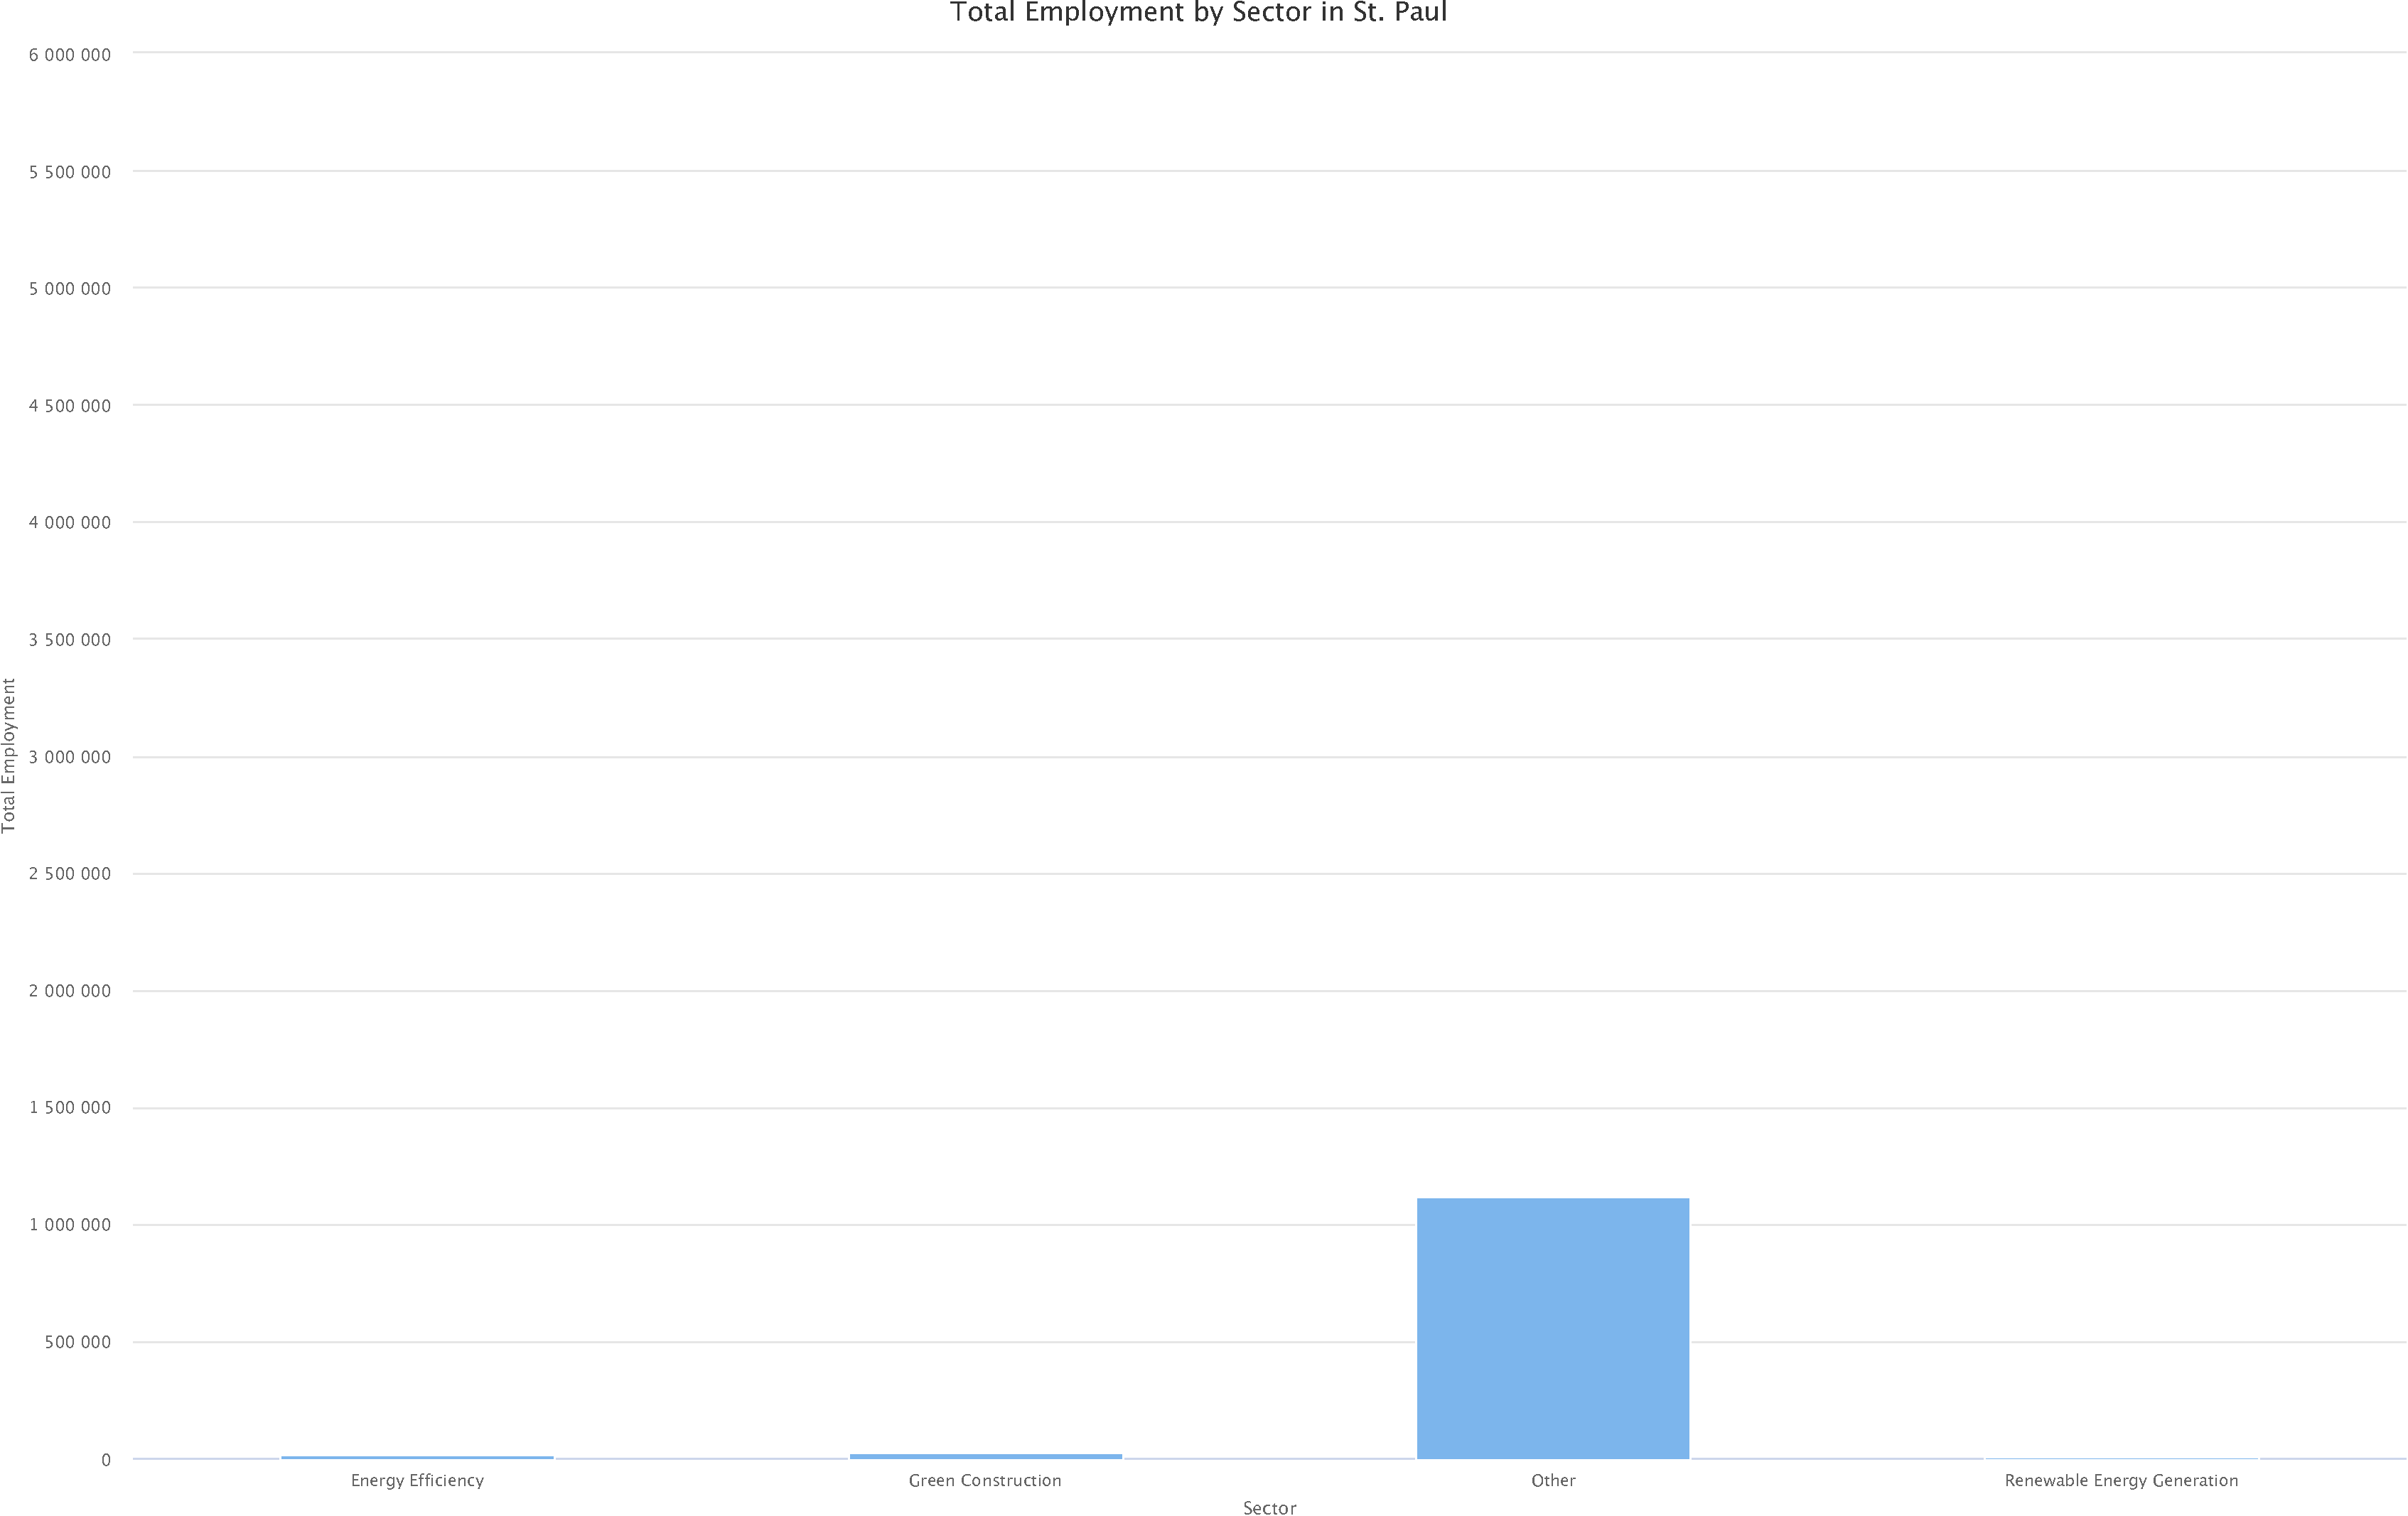
\includegraphics{index_files/figure-pdf/unnamed-chunk-36-1.pdf}

\begin{Shaded}
\begin{Highlighting}[]
\CommentTok{\# Visualization for Mean Hourly Wage across sectors}
\FunctionTok{hchart}\NormalTok{(sector\_summary\_st\_paul, }\StringTok{"column"}\NormalTok{, }\FunctionTok{hcaes}\NormalTok{(}\AttributeTok{x =} \StringTok{\textasciigrave{}}\AttributeTok{O*NET{-}SOC Sector}\StringTok{\textasciigrave{}}\NormalTok{, }\AttributeTok{y =}\NormalTok{ Mean\_Hourly\_Wage)) }\SpecialCharTok{\%\textgreater{}\%}
  \FunctionTok{hc\_title}\NormalTok{(}\AttributeTok{text =} \StringTok{"Mean Hourly Wage by Sector in St. Paul"}\NormalTok{) }\SpecialCharTok{\%\textgreater{}\%}
  \FunctionTok{hc\_xAxis}\NormalTok{(}\AttributeTok{title =} \FunctionTok{list}\NormalTok{(}\AttributeTok{text =} \StringTok{"Sector"}\NormalTok{)) }\SpecialCharTok{\%\textgreater{}\%}
  \FunctionTok{hc\_yAxis}\NormalTok{(}\AttributeTok{title =} \FunctionTok{list}\NormalTok{(}\AttributeTok{text =} \StringTok{"Mean Hourly Wage (USD)"}\NormalTok{)) }\SpecialCharTok{\%\textgreater{}\%}
  \FunctionTok{hc\_tooltip}\NormalTok{(}\AttributeTok{pointFormat =} \StringTok{\textquotesingle{}\textless{}b\textgreater{}\{point.y:.2f\} USD\textless{}/b\textgreater{}\textquotesingle{}}\NormalTok{)}
\end{Highlighting}
\end{Shaded}

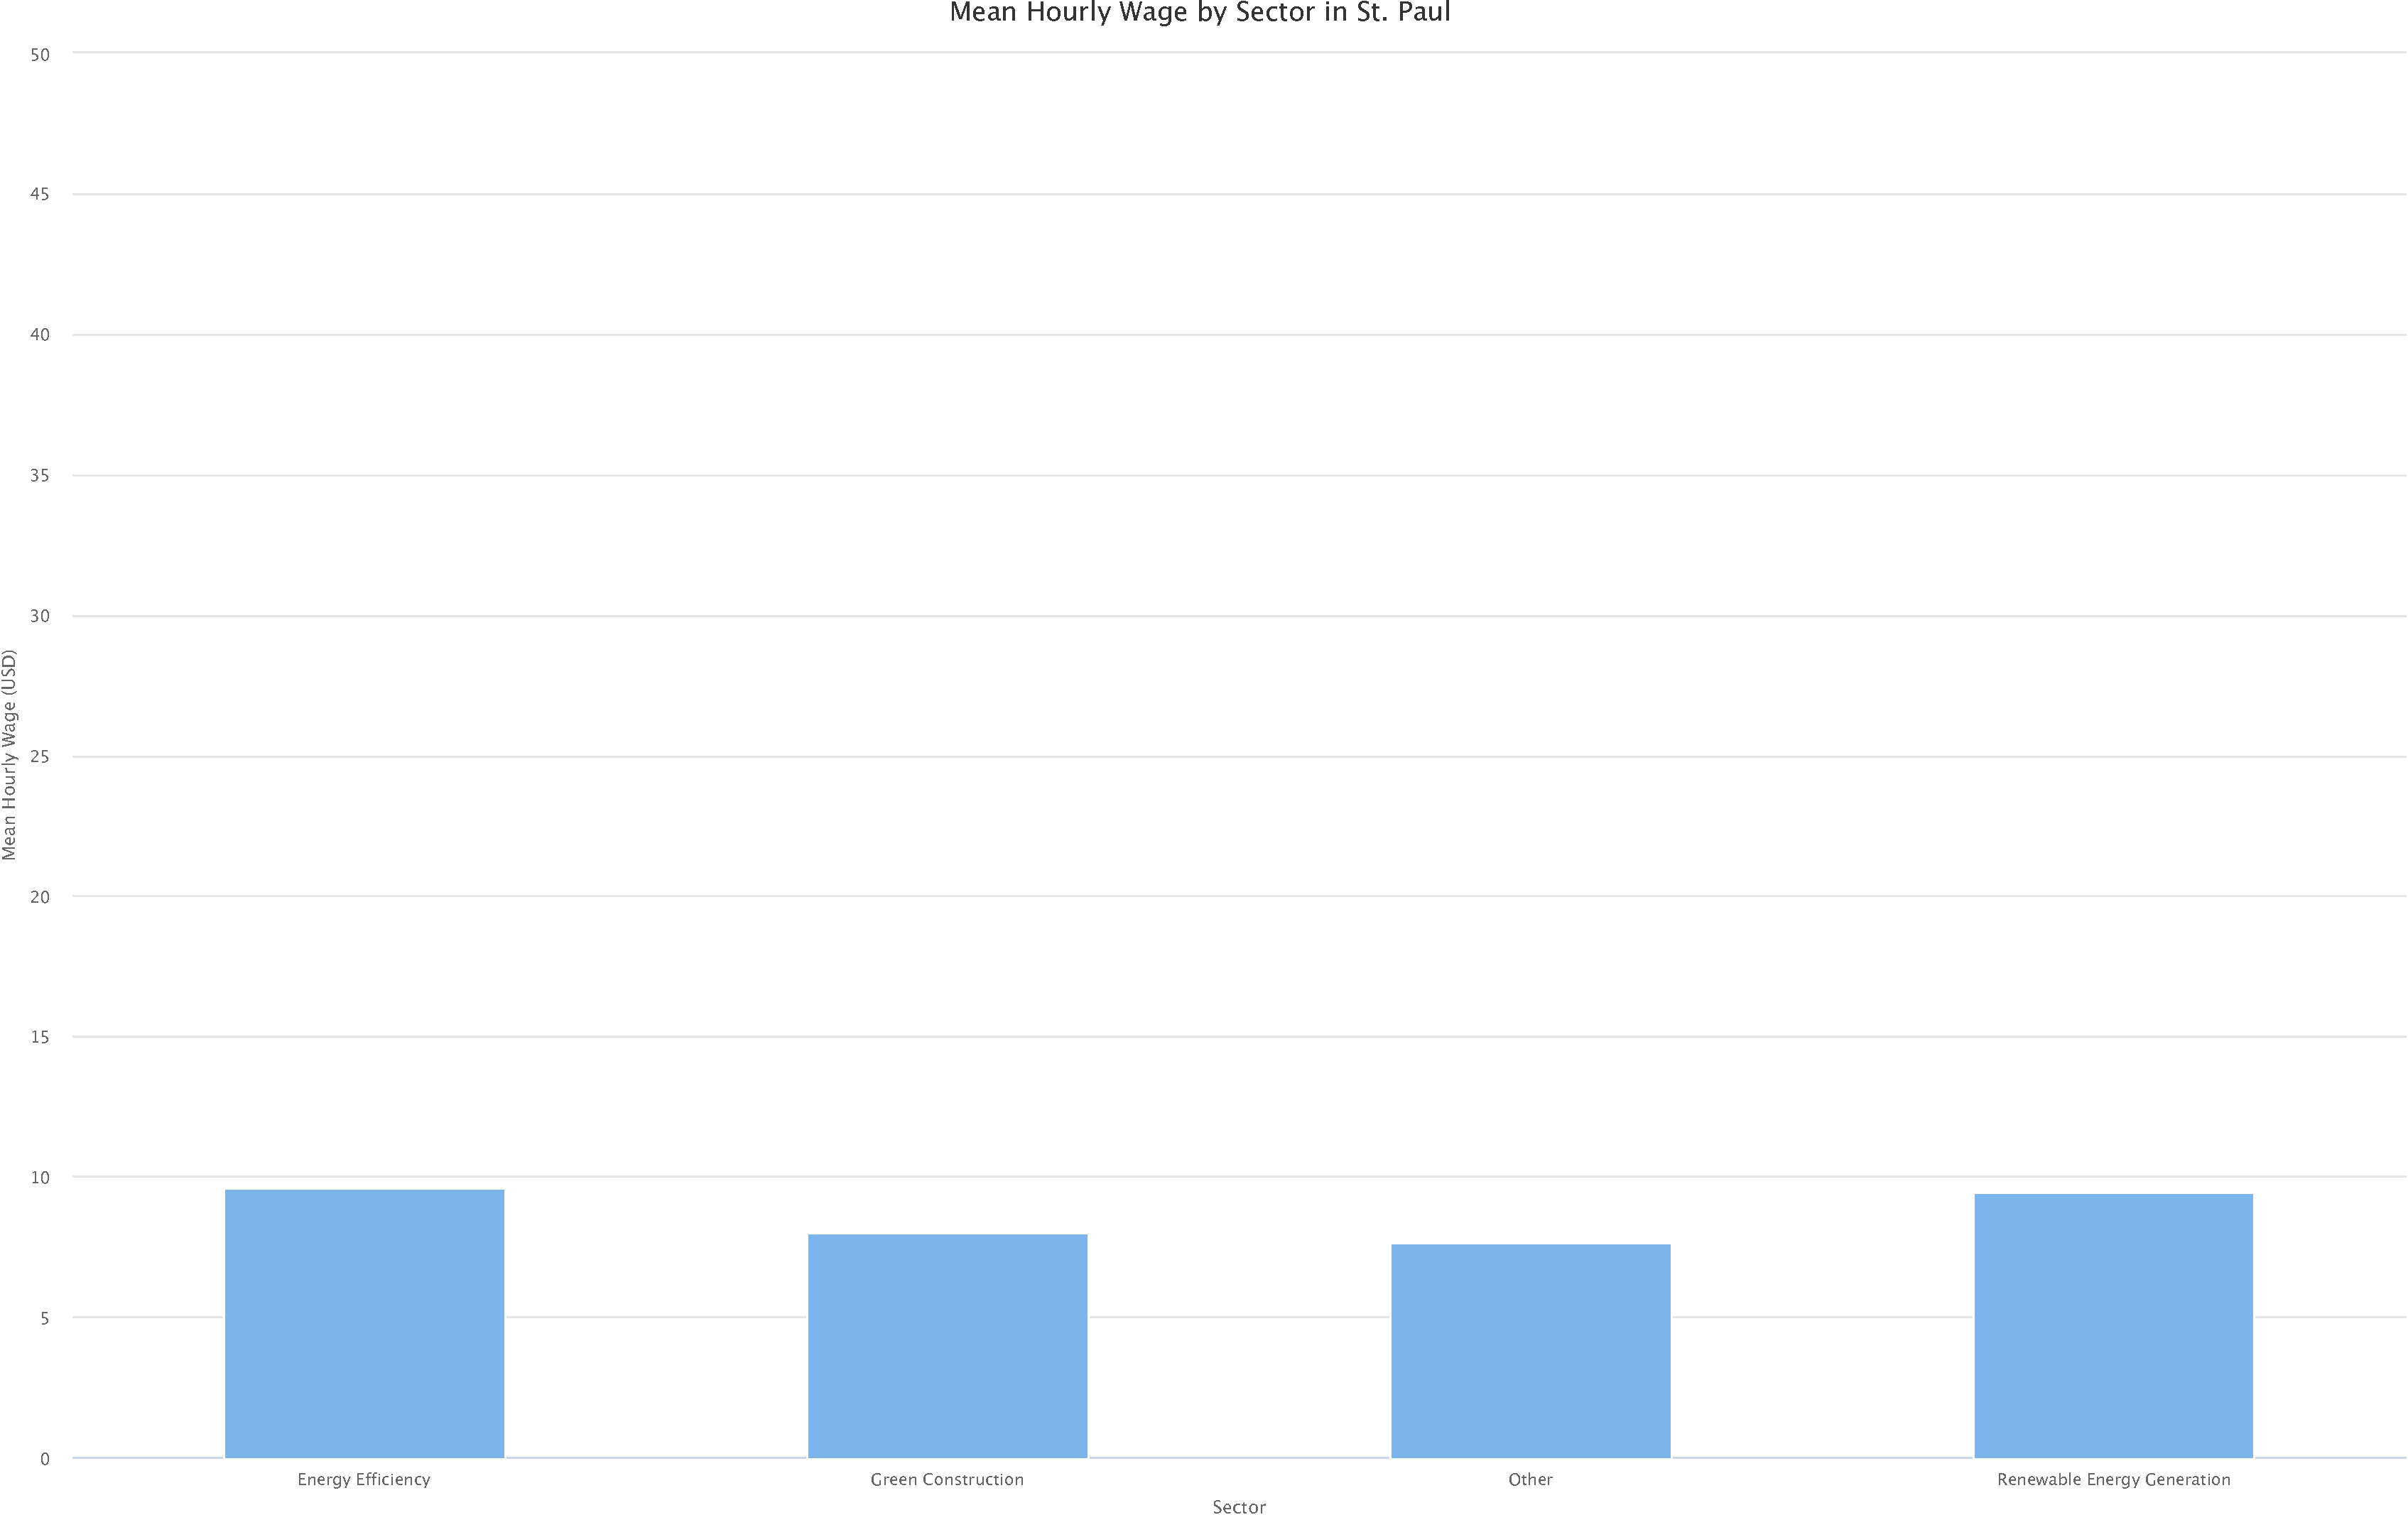
\includegraphics{index_files/figure-pdf/unnamed-chunk-36-2.pdf}

\begin{Shaded}
\begin{Highlighting}[]
\CommentTok{\# Visualization for Mean Annual Wage across sectors}
\FunctionTok{hchart}\NormalTok{(sector\_summary\_st\_paul, }\StringTok{"column"}\NormalTok{, }\FunctionTok{hcaes}\NormalTok{(}\AttributeTok{x =} \StringTok{\textasciigrave{}}\AttributeTok{O*NET{-}SOC Sector}\StringTok{\textasciigrave{}}\NormalTok{, }\AttributeTok{y =}\NormalTok{ Mean\_Annual\_Wage)) }\SpecialCharTok{\%\textgreater{}\%}
  \FunctionTok{hc\_title}\NormalTok{(}\AttributeTok{text =} \StringTok{"Mean Annual Wage by Sector in St. Paul"}\NormalTok{) }\SpecialCharTok{\%\textgreater{}\%}
  \FunctionTok{hc\_xAxis}\NormalTok{(}\AttributeTok{title =} \FunctionTok{list}\NormalTok{(}\AttributeTok{text =} \StringTok{"Sector"}\NormalTok{)) }\SpecialCharTok{\%\textgreater{}\%}
  \FunctionTok{hc\_yAxis}\NormalTok{(}\AttributeTok{title =} \FunctionTok{list}\NormalTok{(}\AttributeTok{text =} \StringTok{"Mean Annual Wage (USD)"}\NormalTok{), }\AttributeTok{labels =} \FunctionTok{list}\NormalTok{(}\AttributeTok{format =} \StringTok{"\{value:,0f\}"}\NormalTok{)) }\SpecialCharTok{\%\textgreater{}\%}
  \FunctionTok{hc\_tooltip}\NormalTok{(}\AttributeTok{pointFormat =} \StringTok{\textquotesingle{}\textless{}b\textgreater{}\{point.y:,0f\} USD\textless{}/b\textgreater{}\textquotesingle{}}\NormalTok{)}
\end{Highlighting}
\end{Shaded}

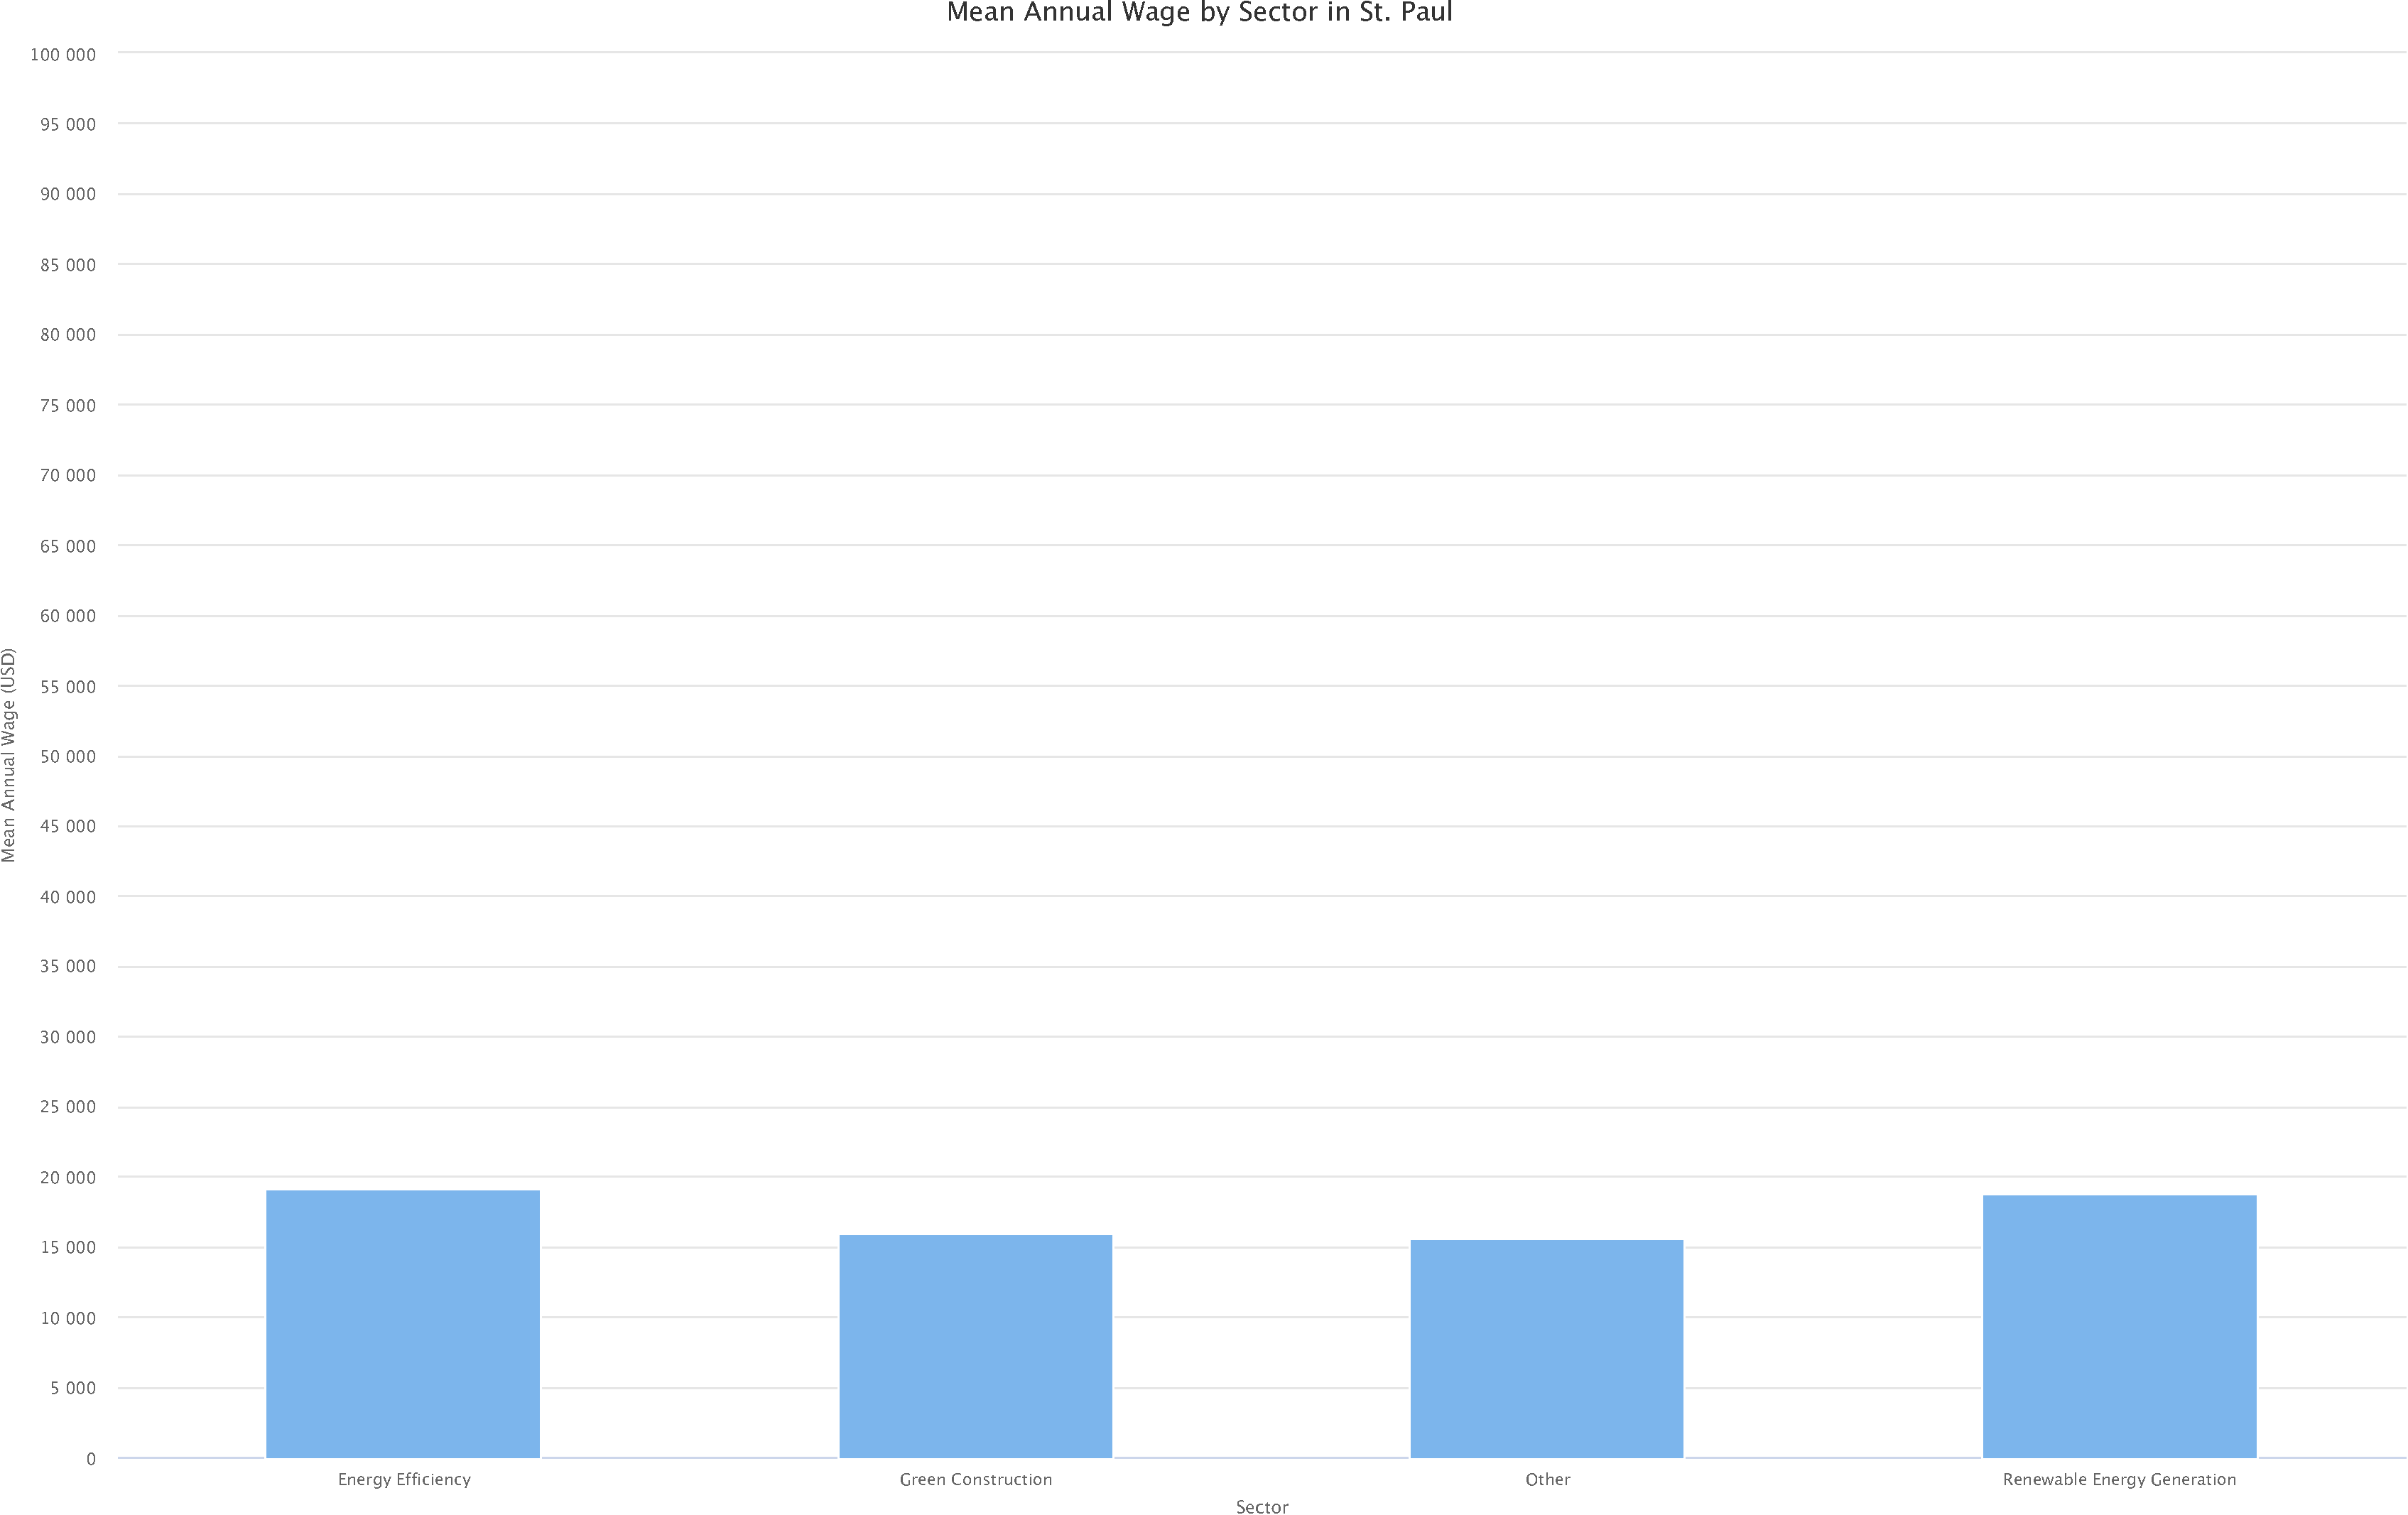
\includegraphics{index_files/figure-pdf/unnamed-chunk-36-3.pdf}

\textsubscript{Source:
\href{https://beeckcenter.github.io/climate-equity-workforce/index-preview.html}{Article
Notebook}}

\textbf{Incorporate ACS demographics}. We will merge the OEWS data with
the \textbf{ACS} data. The \textbf{ACS data} has demographic information
like education, race/ethnicity, gender, and income levels. This will
allow us to analyze the green job data segmented by these demographic
factors in \textbf{St.~Paul}.

\begin{Shaded}
\begin{Highlighting}[]
\CommentTok{\# Convert the O*NET{-}SOC code to character in both datasets}
\NormalTok{st\_paul\_jobs\_weighted }\OtherTok{\textless{}{-}}\NormalTok{ st\_paul\_jobs\_weighted }\SpecialCharTok{\%\textgreater{}\%}
  \FunctionTok{mutate}\NormalTok{(}\StringTok{\textasciigrave{}}\AttributeTok{O*NET{-}SOC Code}\StringTok{\textasciigrave{}} \OtherTok{=} \FunctionTok{as.character}\NormalTok{(}\StringTok{\textasciigrave{}}\AttributeTok{O*NET{-}SOC Code}\StringTok{\textasciigrave{}}\NormalTok{))}

\NormalTok{acs\_data }\OtherTok{\textless{}{-}}\NormalTok{ acs\_data }\SpecialCharTok{\%\textgreater{}\%}
  \FunctionTok{mutate}\NormalTok{(}\StringTok{\textasciigrave{}}\AttributeTok{O*NET{-}SOC Code}\StringTok{\textasciigrave{}} \OtherTok{=} \FunctionTok{as.character}\NormalTok{(}\StringTok{\textasciigrave{}}\AttributeTok{O*NET{-}SOC Code}\StringTok{\textasciigrave{}}\NormalTok{))}
\end{Highlighting}
\end{Shaded}

\textsubscript{Source:
\href{https://beeckcenter.github.io/climate-equity-workforce/index-preview.html}{Article
Notebook}}

\begin{Shaded}
\begin{Highlighting}[]
\CommentTok{\# Filter the ACS data to only include rows where \textquotesingle{}Green Job Flag\textquotesingle{} is 1}
\NormalTok{acs\_green\_data }\OtherTok{\textless{}{-}}\NormalTok{ acs\_data }\SpecialCharTok{\%\textgreater{}\%} 
  \FunctionTok{filter}\NormalTok{(}\StringTok{\textasciigrave{}}\AttributeTok{Green Job Flag}\StringTok{\textasciigrave{}} \SpecialCharTok{==} \DecValTok{1}\NormalTok{)}

\CommentTok{\# Check the filtered data to ensure it looks correct}
\FunctionTok{glimpse}\NormalTok{(acs\_green\_data)}
\end{Highlighting}
\end{Shaded}

\begin{verbatim}
Rows: 72
Columns: 19
$ RT                <chr> "P", "P", "P", "P", "P", "P", "P", "P", "P", "P", "P~
$ SERIALNO          <chr> "2022GQ0001538", "2022GQ0013624", "2022GQ0025479", "~
$ DIVISION          <dbl> 4, 4, 4, 4, 4, 4, 4, 4, 4, 4, 4, 4, 4, 4, 4, 4, 4, 4~
$ SPORDER           <dbl> 1, 1, 1, 1, 1, 1, 1, 1, 1, 1, 1, 2, 5, 1, 1, 2, 2, 2~
$ PUMA20            <dbl> 1505, 1504, 1504, 1503, 1503, 1505, 1504, 1504, 1504~
$ REGION            <dbl> 2, 2, 2, 2, 2, 2, 2, 2, 2, 2, 2, 2, 2, 2, 2, 2, 2, 2~
$ ST                <dbl> 27, 27, 27, 27, 27, 27, 27, 27, 27, 27, 27, 27, 27, ~
$ AGEP              <dbl> 54, 19, 18, 50, 20, 42, 18, 18, 50, 20, 21, 67, 45, ~
$ SOCP              <chr> "472181", "537062", "537062", "537062", "537062", "4~
$ RAC1P             <chr> "White alone", "Asian alone", "Two or More Races", "~
$ SEX               <chr> "Male", "Male", "Male", "Male", "Male", "Male", "Mal~
$ SCHL              <chr> "GED or alternative credential", "Regular high schoo~
$ PINCP             <dbl> 0, 4000, 4000, 19200, 4000, 14700, 4000, 20000, 1920~
$ ADJINC            <dbl> 1042311, 1042311, 1042311, 1042311, 1042311, 1042311~
$ WAGP              <dbl> 0, 4000, 4000, 18000, 4000, 11100, 4000, 20000, 1800~
$ PWGTP             <dbl> 1, 5, 12, 12, 8, 1, 5, 7, 12, 12, 14, 30, 35, 33, 29~
$ `O*NET-SOC Code`  <chr> "472181", "537062", "537062", "537062", "537062", "4~
$ `O*NET-SOC Title` <chr> "Roofers", "Laborers and Freight, Stock, and Materia~
$ `Green Job Flag`  <dbl> 1, 1, 1, 1, 1, 1, 1, 1, 1, 1, 1, 1, 1, 1, 1, 1, 1, 1~
\end{verbatim}

\textsubscript{Source:
\href{https://beeckcenter.github.io/climate-equity-workforce/index-preview.html}{Article
Notebook}}

\begin{Shaded}
\begin{Highlighting}[]
\CommentTok{\# Remove rows with NA O*NET{-}SOC Codes in both datasets before merging}
\NormalTok{st\_paul\_jobs\_weighted }\OtherTok{\textless{}{-}}\NormalTok{ st\_paul\_jobs\_weighted }\SpecialCharTok{\%\textgreater{}\%}
  \FunctionTok{filter}\NormalTok{(}\SpecialCharTok{!}\FunctionTok{is.na}\NormalTok{(}\StringTok{\textasciigrave{}}\AttributeTok{O*NET{-}SOC Code}\StringTok{\textasciigrave{}}\NormalTok{))}

\NormalTok{acs\_green\_data }\OtherTok{\textless{}{-}}\NormalTok{ acs\_green\_data }\SpecialCharTok{\%\textgreater{}\%}
  \FunctionTok{filter}\NormalTok{(}\SpecialCharTok{!}\FunctionTok{is.na}\NormalTok{(}\StringTok{\textasciigrave{}}\AttributeTok{O*NET{-}SOC Code}\StringTok{\textasciigrave{}}\NormalTok{))}

\CommentTok{\# Re{-}check the unique O*NET{-}SOC Codes after filtering out NA values}
\NormalTok{unique\_jobs\_codes }\OtherTok{\textless{}{-}} \FunctionTok{unique}\NormalTok{(st\_paul\_jobs\_weighted}\SpecialCharTok{$}\StringTok{\textasciigrave{}}\AttributeTok{O*NET{-}SOC Code}\StringTok{\textasciigrave{}}\NormalTok{)}
\NormalTok{unique\_acs\_codes }\OtherTok{\textless{}{-}} \FunctionTok{unique}\NormalTok{(acs\_green\_data}\SpecialCharTok{$}\StringTok{\textasciigrave{}}\AttributeTok{O*NET{-}SOC Code}\StringTok{\textasciigrave{}}\NormalTok{)}

\CommentTok{\# Find codes that exist in one dataset but not the other}
\NormalTok{missing\_in\_acs }\OtherTok{\textless{}{-}} \FunctionTok{setdiff}\NormalTok{(unique\_jobs\_codes, unique\_acs\_codes)}
\NormalTok{missing\_in\_jobs }\OtherTok{\textless{}{-}} \FunctionTok{setdiff}\NormalTok{(unique\_acs\_codes, unique\_jobs\_codes)}

\CommentTok{\# Output the results}
\FunctionTok{cat}\NormalTok{(}\StringTok{"Codes in jobs but not in ACS:"}\NormalTok{, missing\_in\_acs, }\StringTok{"}\SpecialCharTok{\textbackslash{}n}\StringTok{"}\NormalTok{)}
\end{Highlighting}
\end{Shaded}

\begin{verbatim}
Codes in jobs but not in ACS: 11-1021 11-3071 11-9021 13-2051 17-1011 17-1012 17-2051 17-2071 17-2141 17-3011 19-3051 47-2011 47-2031 47-2051 47-2061 47-2073 47-2111 47-2131 47-2152 47-2181 47-2211 47-2221 47-4011 47-4041 49-9021 49-9051 49-9098 51-2041 51-4041 51-4121 51-8012 51-8013 51-8021 51-9012 53-6051 53-7051 53-7062 47-5041 49-9042 19-4051 51-8011 19-4041 47-5013 13-1073 47-3012 
\end{verbatim}

\begin{Shaded}
\begin{Highlighting}[]
\FunctionTok{cat}\NormalTok{(}\StringTok{"Codes in ACS but not in jobs:"}\NormalTok{, missing\_in\_jobs, }\StringTok{"}\SpecialCharTok{\textbackslash{}n}\StringTok{"}\NormalTok{)}
\end{Highlighting}
\end{Shaded}

\begin{verbatim}
Codes in ACS but not in jobs: 472181 537062 472061 514041 111021 472111 132051 537051 172141 172051 472152 472031 474011 113071 171011 119021 518021 
\end{verbatim}

\begin{Shaded}
\begin{Highlighting}[]
\CommentTok{\# Ensure the O*NET{-}SOC Code format is consistent}
\CommentTok{\# Remove hyphens from the codes in both datasets for consistent matching}
\NormalTok{st\_paul\_jobs\_weighted }\OtherTok{\textless{}{-}}\NormalTok{ st\_paul\_jobs\_weighted }\SpecialCharTok{\%\textgreater{}\%}
  \FunctionTok{mutate}\NormalTok{(}\StringTok{\textasciigrave{}}\AttributeTok{O*NET{-}SOC Code}\StringTok{\textasciigrave{}} \OtherTok{=} \FunctionTok{gsub}\NormalTok{(}\StringTok{"{-}"}\NormalTok{, }\StringTok{""}\NormalTok{, }\StringTok{\textasciigrave{}}\AttributeTok{O*NET{-}SOC Code}\StringTok{\textasciigrave{}}\NormalTok{))}

\NormalTok{acs\_green\_data }\OtherTok{\textless{}{-}}\NormalTok{ acs\_green\_data }\SpecialCharTok{\%\textgreater{}\%}
  \FunctionTok{mutate}\NormalTok{(}\StringTok{\textasciigrave{}}\AttributeTok{O*NET{-}SOC Code}\StringTok{\textasciigrave{}} \OtherTok{=} \FunctionTok{gsub}\NormalTok{(}\StringTok{"{-}"}\NormalTok{, }\StringTok{""}\NormalTok{, }\StringTok{\textasciigrave{}}\AttributeTok{O*NET{-}SOC Code}\StringTok{\textasciigrave{}}\NormalTok{))}

\CommentTok{\# Re{-}check the unique O*NET{-}SOC Codes after formatting}
\NormalTok{unique\_jobs\_codes }\OtherTok{\textless{}{-}} \FunctionTok{unique}\NormalTok{(st\_paul\_jobs\_weighted}\SpecialCharTok{$}\StringTok{\textasciigrave{}}\AttributeTok{O*NET{-}SOC Code}\StringTok{\textasciigrave{}}\NormalTok{)}
\NormalTok{unique\_acs\_codes }\OtherTok{\textless{}{-}} \FunctionTok{unique}\NormalTok{(acs\_green\_data}\SpecialCharTok{$}\StringTok{\textasciigrave{}}\AttributeTok{O*NET{-}SOC Code}\StringTok{\textasciigrave{}}\NormalTok{)}

\CommentTok{\# Find codes that exist in one dataset but not the other}
\NormalTok{missing\_in\_acs }\OtherTok{\textless{}{-}} \FunctionTok{setdiff}\NormalTok{(unique\_jobs\_codes, unique\_acs\_codes)}
\NormalTok{missing\_in\_jobs }\OtherTok{\textless{}{-}} \FunctionTok{setdiff}\NormalTok{(unique\_acs\_codes, unique\_jobs\_codes)}

\CommentTok{\# Output the results}
\FunctionTok{cat}\NormalTok{(}\StringTok{"Codes in jobs but not in ACS:"}\NormalTok{, missing\_in\_acs, }\StringTok{"}\SpecialCharTok{\textbackslash{}n}\StringTok{"}\NormalTok{)}
\end{Highlighting}
\end{Shaded}

\begin{verbatim}
Codes in jobs but not in ACS: 171012 172071 173011 193051 472011 472051 472073 472131 472211 472221 474041 499021 499051 499098 512041 514121 518012 518013 519012 536051 475041 499042 194051 518011 194041 475013 131073 473012 
\end{verbatim}

\begin{Shaded}
\begin{Highlighting}[]
\FunctionTok{cat}\NormalTok{(}\StringTok{"Codes in ACS but not in jobs:"}\NormalTok{, missing\_in\_jobs, }\StringTok{"}\SpecialCharTok{\textbackslash{}n}\StringTok{"}\NormalTok{)}
\end{Highlighting}
\end{Shaded}

\begin{verbatim}
Codes in ACS but not in jobs:  
\end{verbatim}

\textsubscript{Source:
\href{https://beeckcenter.github.io/climate-equity-workforce/index-preview.html}{Article
Notebook}}

\begin{Shaded}
\begin{Highlighting}[]
\CommentTok{\# Merge the \textquotesingle{}st\_paul\_jobs\_weighted\textquotesingle{} data with \textquotesingle{}acs\_green\_data\textquotesingle{} using the \textquotesingle{}O*NET{-}SOC Code\textquotesingle{} column}
\NormalTok{merged\_green\_jobs\_data }\OtherTok{\textless{}{-}}\NormalTok{ st\_paul\_jobs\_weighted }\SpecialCharTok{\%\textgreater{}\%}
  \FunctionTok{left\_join}\NormalTok{(acs\_green\_data, }\AttributeTok{by =} \StringTok{"O*NET{-}SOC Code"}\NormalTok{)}
\end{Highlighting}
\end{Shaded}

\begin{verbatim}
Warning in left_join(., acs_green_data, by = "O*NET-SOC Code"): Detected an unexpected many-to-many relationship between `x` and `y`.
i Row 1 of `x` matches multiple rows in `y`.
i Row 17 of `y` matches multiple rows in `x`.
i If a many-to-many relationship is expected, set `relationship =
  "many-to-many"` to silence this warning.
\end{verbatim}

\begin{Shaded}
\begin{Highlighting}[]
\CommentTok{\# Check the merged data to validate the merge}
\FunctionTok{glimpse}\NormalTok{(merged\_green\_jobs\_data)}
\end{Highlighting}
\end{Shaded}

\begin{verbatim}
Rows: 124
Columns: 55
$ AREA               <dbl> 33460, 33460, 33460, 33460, 33460, 33460, 33460, 33~
$ AREA_TITLE         <chr> "Minneapolis-St. Paul-Bloomington, MN-WI", "Minneap~
$ AREA_TYPE          <dbl> 4, 4, 4, 4, 4, 4, 4, 4, 4, 4, 4, 4, 4, 4, 4, 4, 4, ~
$ PRIM_STATE         <chr> "MN", "MN", "MN", "MN", "MN", "MN", "MN", "MN", "MN~
$ NAICS              <dbl> 0, 0, 0, 0, 0, 0, 0, 0, 0, 0, 0, 0, 0, 0, 0, 0, 0, ~
$ NAICS_TITLE        <chr> "Cross-industry", "Cross-industry", "Cross-industry~
$ I_GROUP            <chr> "cross-industry", "cross-industry", "cross-industry~
$ OWN_CODE           <dbl> 1235, 1235, 1235, 1235, 1235, 1235, 1235, 1235, 123~
$ OCC_CODE           <chr> "11-1021", "11-1021", "11-1021", "11-1021", "11-102~
$ OCC_TITLE          <chr> "General and Operations Managers", "General and Ope~
$ O_GROUP            <chr> "detailed", "detailed", "detailed", "detailed", "de~
$ TOT_EMP            <dbl> 48300, 48300, 48300, 48300, 48300, 48300, 2610, 261~
$ EMP_PRSE           <chr> "2", "2", "2", "2", "2", "2", "3.1", "3.1", "3.1", ~
$ JOBS_1000          <chr> "25.272", "25.272", "25.272", "25.272", "25.272", "~
$ LOC_QUOTIENT       <chr> "1.09", "1.09", "1.09", "1.09", "1.09", "1.09", "1.~
$ PCT_TOTAL          <lgl> NA, NA, NA, NA, NA, NA, NA, NA, NA, NA, NA, NA, NA,~
$ PCT_RPT            <lgl> NA, NA, NA, NA, NA, NA, NA, NA, NA, NA, NA, NA, NA,~
$ H_MEAN             <dbl> 59.93, 59.93, 59.93, 59.93, 59.93, 59.93, 61.90, 61~
$ A_MEAN             <dbl> 124650, 124650, 124650, 124650, 124650, 124650, 128~
$ MEAN_PRSE          <chr> "1.2", "1.2", "1.2", "1.2", "1.2", "1.2", "1.1", "1~
$ H_PCT10            <chr> "22.92", "22.92", "22.92", "22.92", "22.92", "22.92~
$ H_PCT25            <chr> "32.21", "32.21", "32.21", "32.21", "32.21", "32.21~
$ H_MEDIAN           <chr> "49.26", "49.26", "49.26", "49.26", "49.26", "49.26~
$ H_PCT75            <chr> "76.63", "76.63", "76.63", "76.63", "76.63", "76.63~
$ H_PCT90            <chr> "105.67", "105.67", "105.67", "105.67", "105.67", "~
$ A_PCT10            <chr> "47670", "47670", "47670", "47670", "47670", "47670~
$ A_PCT25            <chr> "66990", "66990", "66990", "66990", "66990", "66990~
$ A_MEDIAN           <chr> "102460", "102460", "102460", "102460", "102460", "~
$ A_PCT75            <chr> "159380", "159380", "159380", "159380", "159380", "~
$ A_PCT90            <chr> "219800", "219800", "219800", "219800", "219800", "~
$ ANNUAL             <lgl> NA, NA, NA, NA, NA, NA, NA, NA, NA, NA, NA, NA, NA,~
$ HOURLY             <lgl> NA, NA, NA, NA, NA, NA, NA, NA, NA, NA, NA, NA, NA,~
$ `O*NET-SOC Code`   <chr> "111021", "111021", "111021", "111021", "111021", "~
$ `O*NET-SOC Sector` <chr> "Energy Efficiency", "Energy Efficiency", "Energy E~
$ TOT_EMP_St_Paul    <dbl> 48300, 48300, 48300, 48300, 48300, 48300, 2610, 261~
$ H_MEAN_St_Paul     <dbl> 59.93, 59.93, 59.93, 59.93, 59.93, 59.93, 61.90, 61~
$ A_MEAN_St_Paul     <dbl> 124650, 124650, 124650, 124650, 124650, 124650, 128~
$ RT                 <chr> "P", "P", "P", "P", "P", "P", "P", "P", "P", "P", "~
$ SERIALNO           <chr> "2022HU0005354", "2022HU0054042", "2022HU0097062", ~
$ DIVISION           <dbl> 4, 4, 4, 4, 4, 4, 4, 4, 4, 4, 4, 4, 4, 4, 4, 4, 4, ~
$ SPORDER            <dbl> 2, 1, 1, 2, 1, 2, 2, 1, 1, 1, 3, 2, 1, 1, 2, 1, 1, ~
$ PUMA20             <dbl> 1504, 1504, 1505, 1504, 1505, 1504, 1505, 1505, 150~
$ REGION             <dbl> 2, 2, 2, 2, 2, 2, 2, 2, 2, 2, 2, 2, 2, 2, 2, 2, 2, ~
$ ST                 <dbl> 27, 27, 27, 27, 27, 27, 27, 27, 27, 27, 27, 27, 27,~
$ AGEP               <dbl> 67, 35, 30, 46, 64, 37, 51, 39, 22, 34, 26, 31, 60,~
$ SOCP               <chr> "111021", "111021", "111021", "111021", "111021", "~
$ RAC1P              <chr> "White alone", "White alone", "Black or African Ame~
$ SEX                <chr> "Male", "Female", "Male", "Female", "Female", "Male~
$ SCHL               <chr> "1 or more years of college credit, no degree", "Ba~
$ PINCP              <dbl> 41000, 50000, 38000, 30000, 0, 94000, 68000, 120000~
$ ADJINC             <dbl> 1042311, 1042311, 1042311, 1042311, 1042311, 104231~
$ WAGP               <dbl> 14000, 50000, 38000, 0, 0, 94000, 68000, 120000, 20~
$ PWGTP              <dbl> 30, 29, 175, 25, 12, 25, 18, 35, 14, 28, 76, 27, 32~
$ `O*NET-SOC Title`  <chr> "General and Operations Managers", "General and Ope~
$ `Green Job Flag`   <dbl> 1, 1, 1, 1, 1, 1, 1, 1, 1, 1, 1, 1, 1, 1, 1, 1, 1, ~
\end{verbatim}

\begin{Shaded}
\begin{Highlighting}[]
\CommentTok{\# Save the merged dataset for future reference}
\FunctionTok{saveRDS}\NormalTok{(merged\_green\_jobs\_data, }\FunctionTok{here}\NormalTok{(}\StringTok{"processed\_data"}\NormalTok{, }\StringTok{"merged\_green\_jobs\_data.rds"}\NormalTok{))}
\FunctionTok{write\_csv}\NormalTok{(merged\_green\_jobs\_data, }\FunctionTok{here}\NormalTok{(}\StringTok{"processed\_data"}\NormalTok{, }\StringTok{"merged\_green\_jobs\_data.csv"}\NormalTok{))}
\end{Highlighting}
\end{Shaded}

\textsubscript{Source:
\href{https://beeckcenter.github.io/climate-equity-workforce/index-preview.html}{Article
Notebook}}

\begin{Shaded}
\begin{Highlighting}[]
\CommentTok{\# Assess the number of duplicates in the merged dataset by counting occurrences of each O*NET{-}SOC Code}
\NormalTok{duplication\_summary }\OtherTok{\textless{}{-}}\NormalTok{ merged\_green\_jobs\_data }\SpecialCharTok{\%\textgreater{}\%}
  \FunctionTok{group\_by}\NormalTok{(}\StringTok{\textasciigrave{}}\AttributeTok{O*NET{-}SOC Code}\StringTok{\textasciigrave{}}\NormalTok{) }\SpecialCharTok{\%\textgreater{}\%}
  \FunctionTok{summarise}\NormalTok{(}\AttributeTok{count =} \FunctionTok{n}\NormalTok{()) }\SpecialCharTok{\%\textgreater{}\%}
  \FunctionTok{arrange}\NormalTok{(}\FunctionTok{desc}\NormalTok{(count))}

\CommentTok{\# View the summary of duplication}
\FunctionTok{print}\NormalTok{(duplication\_summary)}
\end{Highlighting}
\end{Shaded}

\begin{verbatim}
# A tibble: 45 x 2
   `O*NET-SOC Code` count
   <chr>            <int>
 1 537062              21
 2 172141              12
 3 472061               8
 4 472111               7
 5 111021               6
 6 132051               6
 7 172051               6
 8 113071               3
 9 171011               3
10 172071               3
# i 35 more rows
\end{verbatim}

\textsubscript{Source:
\href{https://beeckcenter.github.io/climate-equity-workforce/index-preview.html}{Article
Notebook}}

If we need accurate totals or averages across jobs and demographics,
\textbf{aggregation} will be necessary to avoid inflating the data.

If we feel the current level of detail (with the duplicates) provides
useful insights, we can keep the data as is but be mindful of how you
interpret summed metrics. This is what we will do. The duplication is
meaningful (for example, because a job can truly exist in multiple
sectors or demographics are validly associated with multiple jobs), we
choose to keep the dataset as is. This would allow us to analyze the
data with all the overlaps. However, we need to be cautious that this
doesn\textquotesingle t skew metrics that sum values (like total
employment).

\begin{Shaded}
\begin{Highlighting}[]
\CommentTok{\# \# Aggregate demographic and job{-}related data by O*NET{-}SOC Code and O*NET{-}SOC Sector after merge}
\CommentTok{\# aggregated\_data \textless{}{-} merged\_green\_jobs\_data \%\textgreater{}\%}
\CommentTok{\#   group\_by(\textasciigrave{}O*NET{-}SOC Code\textasciigrave{}, \textasciigrave{}O*NET{-}SOC Sector\textasciigrave{}, \textasciigrave{}O*NET{-}SOC Title\textasciigrave{}) \%\textgreater{}\%}
\CommentTok{\#   summarise(}
\CommentTok{\#     Total\_Employment = sum(TOT\_EMP\_St\_Paul, na.rm = TRUE),}
\CommentTok{\#     Mean\_Hourly\_Wage = mean(H\_MEAN\_St\_Paul, na.rm = TRUE),}
\CommentTok{\#     Mean\_Annual\_Wage = mean(A\_MEAN\_St\_Paul, na.rm = TRUE),}
\CommentTok{\#     Average\_Age = mean(AGEP, na.rm = TRUE),}
\CommentTok{\#     Proportion\_Female = mean(SEX == "Female", na.rm = TRUE),}
\CommentTok{\#     Proportion\_Male = mean(SEX == "Male", na.rm = TRUE),}
\CommentTok{\#     Average\_Income = mean(PINCP, na.rm = TRUE),}
\CommentTok{\#     Proportion\_White = mean(RAC1P == "White alone", na.rm = TRUE),}
\CommentTok{\#     Proportion\_Black = mean(RAC1P == "Black or African American alone", na.rm = TRUE),}
\CommentTok{\#     Count = n()  \# This column helps you see how many records were combined in this aggregation}
\CommentTok{\#   )}
\CommentTok{\# }
\CommentTok{\# \# View the aggregated data}
\CommentTok{\# glimpse(aggregated\_data)}
\end{Highlighting}
\end{Shaded}

\textsubscript{Source:
\href{https://beeckcenter.github.io/climate-equity-workforce/index-preview.html}{Article
Notebook}}

\textbf{Analyze the data}. Once the datasets are merged, you can start
analyzing the data to answer your research question.

Now that we've merged the \textbf{OEWS} and \textbf{ACS} data, we can
group by the \textbf{O*NET-SOC Sector} (Energy Efficiency, Renewable
Energy Generation, Green Construction) and demographic factors like
\textbf{education}, \textbf{race}, \textbf{gender}, and \textbf{income}.

\begin{Shaded}
\begin{Highlighting}[]
\CommentTok{\# Convert data types}
\NormalTok{merged\_green\_jobs\_data }\OtherTok{\textless{}{-}}\NormalTok{ merged\_green\_jobs\_data }\SpecialCharTok{\%\textgreater{}\%}
  \FunctionTok{mutate}\NormalTok{(}
    \AttributeTok{NAICS\_TITLE =} \FunctionTok{as.factor}\NormalTok{(NAICS\_TITLE),  }\CommentTok{\# Factor for industry titles}
    \AttributeTok{I\_GROUP =} \FunctionTok{as.factor}\NormalTok{(I\_GROUP),  }\CommentTok{\# Factor for industry group}
    \AttributeTok{O\_GROUP =} \FunctionTok{as.factor}\NormalTok{(O\_GROUP),  }\CommentTok{\# Factor for occupation group}
    \AttributeTok{H\_PCT10 =} \FunctionTok{as.numeric}\NormalTok{(H\_PCT10),  }\CommentTok{\# Convert percentages to numeric}
    \AttributeTok{H\_PCT25 =} \FunctionTok{as.numeric}\NormalTok{(H\_PCT25),}
    \AttributeTok{H\_MEDIAN =} \FunctionTok{as.numeric}\NormalTok{(H\_MEDIAN),}
    \AttributeTok{H\_PCT75 =} \FunctionTok{as.numeric}\NormalTok{(H\_PCT75),}
    \AttributeTok{H\_PCT90 =} \FunctionTok{as.numeric}\NormalTok{(H\_PCT90),}
    \AttributeTok{A\_PCT10 =} \FunctionTok{as.numeric}\NormalTok{(A\_PCT10),}
    \AttributeTok{A\_PCT25 =} \FunctionTok{as.numeric}\NormalTok{(A\_PCT25),}
    \AttributeTok{A\_MEDIAN =} \FunctionTok{as.numeric}\NormalTok{(A\_MEDIAN),}
    \AttributeTok{A\_PCT75 =} \FunctionTok{as.numeric}\NormalTok{(A\_PCT75),}
    \AttributeTok{A\_PCT90 =} \FunctionTok{as.numeric}\NormalTok{(A\_PCT90),}
    \AttributeTok{ANNUAL =} \FunctionTok{as.numeric}\NormalTok{(ANNUAL),  }\CommentTok{\# Convert to numeric for consistency}
    \AttributeTok{HOURLY =} \FunctionTok{as.numeric}\NormalTok{(HOURLY),}
    \StringTok{\textasciigrave{}}\AttributeTok{O*NET{-}SOC Sector}\StringTok{\textasciigrave{}} \OtherTok{=} \FunctionTok{as.factor}\NormalTok{(}\StringTok{\textasciigrave{}}\AttributeTok{O*NET{-}SOC Sector}\StringTok{\textasciigrave{}}\NormalTok{),  }\CommentTok{\# Factor for green job sectors}
    \AttributeTok{TOT\_EMP\_St\_Paul =} \FunctionTok{as.numeric}\NormalTok{(TOT\_EMP\_St\_Paul),  }\CommentTok{\# Numeric for employment totals}
    \AttributeTok{H\_MEAN\_St\_Paul =} \FunctionTok{as.numeric}\NormalTok{(H\_MEAN\_St\_Paul),  }\CommentTok{\# Numeric for hourly wage in St. Paul}
    \AttributeTok{A\_MEAN\_St\_Paul =} \FunctionTok{as.numeric}\NormalTok{(A\_MEAN\_St\_Paul),  }\CommentTok{\# Numeric for annual wage in St. Paul}
    \AttributeTok{AGEP =} \FunctionTok{as.factor}\NormalTok{(AGEP),  }\CommentTok{\# Age as a factor if we treat it categorically}
    \AttributeTok{RAC1P =} \FunctionTok{as.factor}\NormalTok{(RAC1P),  }\CommentTok{\# Factor for race}
    \AttributeTok{SEX =} \FunctionTok{as.factor}\NormalTok{(SEX),  }\CommentTok{\# Factor for gender}
    \AttributeTok{SCHL =} \FunctionTok{as.factor}\NormalTok{(SCHL),  }\CommentTok{\# Factor for education level}
    \AttributeTok{PINCP =} \FunctionTok{as.numeric}\NormalTok{(PINCP),  }\CommentTok{\# Numeric for personal income}
    \AttributeTok{ADJINC =} \FunctionTok{as.numeric}\NormalTok{(ADJINC),  }\CommentTok{\# Numeric for adjusted income}
    \AttributeTok{WAGP =} \FunctionTok{as.numeric}\NormalTok{(WAGP),  }\CommentTok{\# Numeric for wage}
    \AttributeTok{PWGTP =} \FunctionTok{as.numeric}\NormalTok{(PWGTP),  }\CommentTok{\# Numeric for person weight}
    \StringTok{\textasciigrave{}}\AttributeTok{Green Job Flag}\StringTok{\textasciigrave{}} \OtherTok{=} \FunctionTok{as.numeric}\NormalTok{(}\StringTok{\textasciigrave{}}\AttributeTok{Green Job Flag}\StringTok{\textasciigrave{}}\NormalTok{)  }\CommentTok{\# Yes/No as numeric}
\NormalTok{  )}
\end{Highlighting}
\end{Shaded}

\begin{verbatim}
Warning: There were 10 warnings in `mutate()`.
The first warning was:
i In argument: `H_PCT10 = as.numeric(H_PCT10)`.
Caused by warning:
! NAs introduced by coercion
i Run `dplyr::last_dplyr_warnings()` to see the 9 remaining warnings.
\end{verbatim}

\begin{Shaded}
\begin{Highlighting}[]
\CommentTok{\# Double{-}check the changes}
\FunctionTok{glimpse}\NormalTok{(merged\_green\_jobs\_data)}
\end{Highlighting}
\end{Shaded}

\begin{verbatim}
Rows: 124
Columns: 55
$ AREA               <dbl> 33460, 33460, 33460, 33460, 33460, 33460, 33460, 33~
$ AREA_TITLE         <chr> "Minneapolis-St. Paul-Bloomington, MN-WI", "Minneap~
$ AREA_TYPE          <dbl> 4, 4, 4, 4, 4, 4, 4, 4, 4, 4, 4, 4, 4, 4, 4, 4, 4, ~
$ PRIM_STATE         <chr> "MN", "MN", "MN", "MN", "MN", "MN", "MN", "MN", "MN~
$ NAICS              <dbl> 0, 0, 0, 0, 0, 0, 0, 0, 0, 0, 0, 0, 0, 0, 0, 0, 0, ~
$ NAICS_TITLE        <fct> Cross-industry, Cross-industry, Cross-industry, Cro~
$ I_GROUP            <fct> cross-industry, cross-industry, cross-industry, cro~
$ OWN_CODE           <dbl> 1235, 1235, 1235, 1235, 1235, 1235, 1235, 1235, 123~
$ OCC_CODE           <chr> "11-1021", "11-1021", "11-1021", "11-1021", "11-102~
$ OCC_TITLE          <chr> "General and Operations Managers", "General and Ope~
$ O_GROUP            <fct> detailed, detailed, detailed, detailed, detailed, d~
$ TOT_EMP            <dbl> 48300, 48300, 48300, 48300, 48300, 48300, 2610, 261~
$ EMP_PRSE           <chr> "2", "2", "2", "2", "2", "2", "3.1", "3.1", "3.1", ~
$ JOBS_1000          <chr> "25.272", "25.272", "25.272", "25.272", "25.272", "~
$ LOC_QUOTIENT       <chr> "1.09", "1.09", "1.09", "1.09", "1.09", "1.09", "1.~
$ PCT_TOTAL          <lgl> NA, NA, NA, NA, NA, NA, NA, NA, NA, NA, NA, NA, NA,~
$ PCT_RPT            <lgl> NA, NA, NA, NA, NA, NA, NA, NA, NA, NA, NA, NA, NA,~
$ H_MEAN             <dbl> 59.93, 59.93, 59.93, 59.93, 59.93, 59.93, 61.90, 61~
$ A_MEAN             <dbl> 124650, 124650, 124650, 124650, 124650, 124650, 128~
$ MEAN_PRSE          <chr> "1.2", "1.2", "1.2", "1.2", "1.2", "1.2", "1.1", "1~
$ H_PCT10            <dbl> 22.92, 22.92, 22.92, 22.92, 22.92, 22.92, 32.84, 32~
$ H_PCT25            <dbl> 32.21, 32.21, 32.21, 32.21, 32.21, 32.21, 41.03, 41~
$ H_MEDIAN           <dbl> 49.26, 49.26, 49.26, 49.26, 49.26, 49.26, 53.89, 53~
$ H_PCT75            <dbl> 76.63, 76.63, 76.63, 76.63, 76.63, 76.63, 74.34, 74~
$ H_PCT90            <dbl> 105.67, 105.67, 105.67, 105.67, 105.67, 105.67, 99.~
$ A_PCT10            <dbl> 47670, 47670, 47670, 47670, 47670, 47670, 68310, 68~
$ A_PCT25            <dbl> 66990, 66990, 66990, 66990, 66990, 66990, 85340, 85~
$ A_MEDIAN           <dbl> 102460, 102460, 102460, 102460, 102460, 102460, 112~
$ A_PCT75            <dbl> 159380, 159380, 159380, 159380, 159380, 159380, 154~
$ A_PCT90            <dbl> 219800, 219800, 219800, 219800, 219800, 219800, 207~
$ ANNUAL             <dbl> NA, NA, NA, NA, NA, NA, NA, NA, NA, NA, NA, NA, NA,~
$ HOURLY             <dbl> NA, NA, NA, NA, NA, NA, NA, NA, NA, NA, NA, NA, NA,~
$ `O*NET-SOC Code`   <chr> "111021", "111021", "111021", "111021", "111021", "~
$ `O*NET-SOC Sector` <fct> Energy Efficiency, Energy Efficiency, Energy Effici~
$ TOT_EMP_St_Paul    <dbl> 48300, 48300, 48300, 48300, 48300, 48300, 2610, 261~
$ H_MEAN_St_Paul     <dbl> 59.93, 59.93, 59.93, 59.93, 59.93, 59.93, 61.90, 61~
$ A_MEAN_St_Paul     <dbl> 124650, 124650, 124650, 124650, 124650, 124650, 128~
$ RT                 <chr> "P", "P", "P", "P", "P", "P", "P", "P", "P", "P", "~
$ SERIALNO           <chr> "2022HU0005354", "2022HU0054042", "2022HU0097062", ~
$ DIVISION           <dbl> 4, 4, 4, 4, 4, 4, 4, 4, 4, 4, 4, 4, 4, 4, 4, 4, 4, ~
$ SPORDER            <dbl> 2, 1, 1, 2, 1, 2, 2, 1, 1, 1, 3, 2, 1, 1, 2, 1, 1, ~
$ PUMA20             <dbl> 1504, 1504, 1505, 1504, 1505, 1504, 1505, 1505, 150~
$ REGION             <dbl> 2, 2, 2, 2, 2, 2, 2, 2, 2, 2, 2, 2, 2, 2, 2, 2, 2, ~
$ ST                 <dbl> 27, 27, 27, 27, 27, 27, 27, 27, 27, 27, 27, 27, 27,~
$ AGEP               <fct> 67, 35, 30, 46, 64, 37, 51, 39, 22, 34, 26, 31, 60,~
$ SOCP               <chr> "111021", "111021", "111021", "111021", "111021", "~
$ RAC1P              <fct> White alone, White alone, Black or African American~
$ SEX                <fct> Male, Female, Male, Female, Female, Male, Male, Mal~
$ SCHL               <fct> "1 or more years of college credit, no degree", "Ba~
$ PINCP              <dbl> 41000, 50000, 38000, 30000, 0, 94000, 68000, 120000~
$ ADJINC             <dbl> 1042311, 1042311, 1042311, 1042311, 1042311, 104231~
$ WAGP               <dbl> 14000, 50000, 38000, 0, 0, 94000, 68000, 120000, 20~
$ PWGTP              <dbl> 30, 29, 175, 25, 12, 25, 18, 35, 14, 28, 76, 27, 32~
$ `O*NET-SOC Title`  <chr> "General and Operations Managers", "General and Ope~
$ `Green Job Flag`   <dbl> 1, 1, 1, 1, 1, 1, 1, 1, 1, 1, 1, 1, 1, 1, 1, 1, 1, ~
\end{verbatim}

\textsubscript{Source:
\href{https://beeckcenter.github.io/climate-equity-workforce/index-preview.html}{Article
Notebook}}

To group by the \texttt{O*NET-SOC\ Sector} and demographic factors like
\texttt{education}, \texttt{race}, \texttt{gender}, and \texttt{income},
we can create summary statistics for each sector to analyze how the
green jobs are distributed across different demographic categories.

\begin{Shaded}
\begin{Highlighting}[]
\CommentTok{\# Group the data by sector and demographic variables, then summarize the counts and income}
\NormalTok{green\_job\_summary }\OtherTok{\textless{}{-}}\NormalTok{ merged\_green\_jobs\_data }\SpecialCharTok{\%\textgreater{}\%}
  \FunctionTok{group\_by}\NormalTok{(}\StringTok{\textasciigrave{}}\AttributeTok{O*NET{-}SOC Sector}\StringTok{\textasciigrave{}}\NormalTok{, SCHL, RAC1P, SEX) }\SpecialCharTok{\%\textgreater{}\%}
  \FunctionTok{summarise}\NormalTok{(}
    \AttributeTok{total\_jobs =} \FunctionTok{n}\NormalTok{(),  }\CommentTok{\# Count total jobs}
    \AttributeTok{mean\_income =} \FunctionTok{mean}\NormalTok{(PINCP, }\AttributeTok{na.rm =} \ConstantTok{TRUE}\NormalTok{)  }\CommentTok{\# Calculate mean income for each group}
\NormalTok{  )}
\end{Highlighting}
\end{Shaded}

\begin{verbatim}
`summarise()` has grouped output by 'O*NET-SOC Sector', 'SCHL', 'RAC1P'. You
can override using the `.groups` argument.
\end{verbatim}

\begin{Shaded}
\begin{Highlighting}[]
\CommentTok{\# View the summarized data}
\FunctionTok{print}\NormalTok{(green\_job\_summary)}
\end{Highlighting}
\end{Shaded}

\begin{verbatim}
# A tibble: 52 x 6
# Groups:   O*NET-SOC Sector, SCHL, RAC1P [46]
   `O*NET-SOC Sector` SCHL                    RAC1P SEX   total_jobs mean_income
   <fct>              <fct>                   <fct> <fct>      <int>       <dbl>
 1 Energy Efficiency  1 or more years of col~ Whit~ Fema~          1      15000 
 2 Energy Efficiency  1 or more years of col~ Whit~ Male           1      41000 
 3 Energy Efficiency  Associate's degree      Whit~ Male           1      46500 
 4 Energy Efficiency  Bachelor's degree       Two ~ Fema~          1     102000 
 5 Energy Efficiency  Bachelor's degree       Whit~ Fema~          2      40000 
 6 Energy Efficiency  Bachelor's degree       Whit~ Male           3     126417.
 7 Energy Efficiency  Grade 9                 Whit~ Fema~          1          0 
 8 Energy Efficiency  Master's degree         Asia~ Male           1      80000 
 9 Energy Efficiency  Master's degree         Whit~ Fema~          1     113250 
10 Energy Efficiency  Regular high school di~ Whit~ Male           1      94000 
# i 42 more rows
\end{verbatim}

\textsubscript{Source:
\href{https://beeckcenter.github.io/climate-equity-workforce/index-preview.html}{Article
Notebook}}

\begin{Shaded}
\begin{Highlighting}[]
\CommentTok{\# Remove rows with NA in \textquotesingle{}SCHL\textquotesingle{} or \textquotesingle{}O*NET{-}SOC Sector\textquotesingle{}}
\NormalTok{cleaned\_green\_job\_summary }\OtherTok{\textless{}{-}}\NormalTok{ green\_job\_summary }\SpecialCharTok{\%\textgreater{}\%}
  \FunctionTok{filter}\NormalTok{(}\SpecialCharTok{!}\FunctionTok{is.na}\NormalTok{(SCHL), }\SpecialCharTok{!}\FunctionTok{is.na}\NormalTok{(}\StringTok{\textasciigrave{}}\AttributeTok{O*NET{-}SOC Sector}\StringTok{\textasciigrave{}}\NormalTok{))}

\CommentTok{\# Bar plot for green jobs by sector and education level}
\FunctionTok{ggplot}\NormalTok{(cleaned\_green\_job\_summary, }\FunctionTok{aes}\NormalTok{(}\AttributeTok{x =} \StringTok{\textasciigrave{}}\AttributeTok{O*NET{-}SOC Sector}\StringTok{\textasciigrave{}}\NormalTok{, }\AttributeTok{y =}\NormalTok{ total\_jobs, }\AttributeTok{fill =}\NormalTok{ SCHL)) }\SpecialCharTok{+}
  \FunctionTok{geom\_bar}\NormalTok{(}\AttributeTok{stat =} \StringTok{"identity"}\NormalTok{, }\AttributeTok{position =} \StringTok{"dodge"}\NormalTok{) }\SpecialCharTok{+}
  \FunctionTok{labs}\NormalTok{(}\AttributeTok{title =} \StringTok{"Green Jobs by Sector and Education Level"}\NormalTok{,}
       \AttributeTok{x =} \StringTok{"Green Job Sector"}\NormalTok{, }\AttributeTok{y =} \StringTok{"Total Jobs"}\NormalTok{) }\SpecialCharTok{+}
  \FunctionTok{theme\_minimal}\NormalTok{() }\SpecialCharTok{+}
  \FunctionTok{theme}\NormalTok{(}\AttributeTok{axis.text.x =} \FunctionTok{element\_text}\NormalTok{(}\AttributeTok{angle =} \DecValTok{45}\NormalTok{, }\AttributeTok{hjust =} \DecValTok{1}\NormalTok{))}
\end{Highlighting}
\end{Shaded}

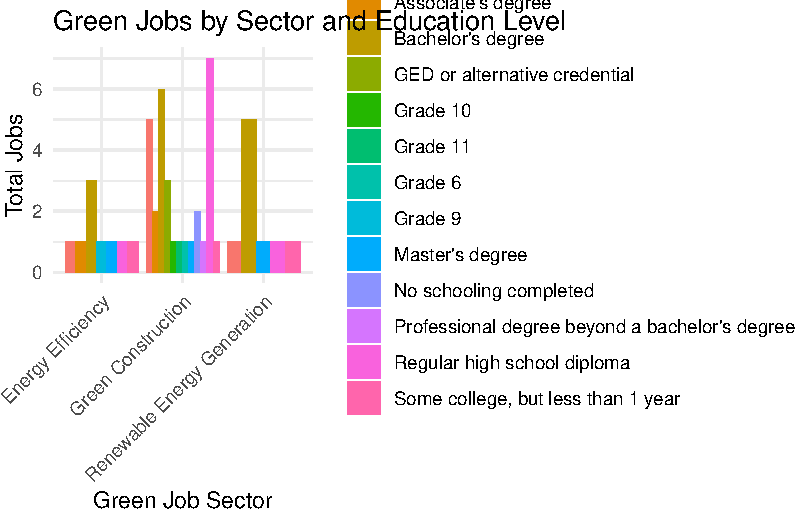
\includegraphics{index_files/figure-pdf/unnamed-chunk-45-1.pdf}

\begin{Shaded}
\begin{Highlighting}[]
\CommentTok{\# Plot percentage of jobs by sector and education level}
\NormalTok{green\_job\_summary\_percentage }\OtherTok{\textless{}{-}}\NormalTok{ merged\_green\_jobs\_data }\SpecialCharTok{\%\textgreater{}\%}
  \FunctionTok{group\_by}\NormalTok{(}\StringTok{\textasciigrave{}}\AttributeTok{O*NET{-}SOC Sector}\StringTok{\textasciigrave{}}\NormalTok{, SCHL) }\SpecialCharTok{\%\textgreater{}\%}
  \FunctionTok{summarise}\NormalTok{(}\AttributeTok{total\_jobs =} \FunctionTok{n}\NormalTok{()) }\SpecialCharTok{\%\textgreater{}\%}
  \FunctionTok{mutate}\NormalTok{(}\AttributeTok{percentage\_jobs =}\NormalTok{ total\_jobs }\SpecialCharTok{/} \FunctionTok{sum}\NormalTok{(total\_jobs) }\SpecialCharTok{*} \DecValTok{100}\NormalTok{)}
\end{Highlighting}
\end{Shaded}

\begin{verbatim}
`summarise()` has grouped output by 'O*NET-SOC Sector'. You can override using
the `.groups` argument.
\end{verbatim}

\begin{Shaded}
\begin{Highlighting}[]
\FunctionTok{ggplot}\NormalTok{(green\_job\_summary\_percentage, }\FunctionTok{aes}\NormalTok{(}\AttributeTok{x =} \StringTok{\textasciigrave{}}\AttributeTok{O*NET{-}SOC Sector}\StringTok{\textasciigrave{}}\NormalTok{, }\AttributeTok{y =}\NormalTok{ percentage\_jobs, }\AttributeTok{fill =}\NormalTok{ SCHL)) }\SpecialCharTok{+}
  \FunctionTok{geom\_bar}\NormalTok{(}\AttributeTok{stat =} \StringTok{"identity"}\NormalTok{, }\AttributeTok{position =} \StringTok{"dodge"}\NormalTok{) }\SpecialCharTok{+}
  \FunctionTok{labs}\NormalTok{(}\AttributeTok{title =} \StringTok{"Percentage of Green Jobs by Sector and Education Level"}\NormalTok{,}
       \AttributeTok{x =} \StringTok{"Green Job Sector"}\NormalTok{, }\AttributeTok{y =} \StringTok{"Percentage of Total Jobs"}\NormalTok{) }\SpecialCharTok{+}
  \FunctionTok{theme\_minimal}\NormalTok{() }\SpecialCharTok{+}
  \FunctionTok{theme}\NormalTok{(}\AttributeTok{axis.text.x =} \FunctionTok{element\_text}\NormalTok{(}\AttributeTok{angle =} \DecValTok{45}\NormalTok{, }\AttributeTok{hjust =} \DecValTok{1}\NormalTok{))}
\end{Highlighting}
\end{Shaded}

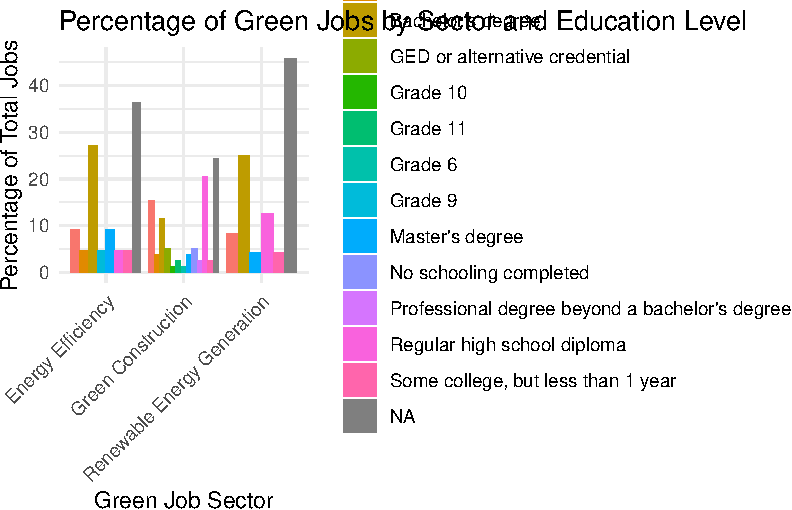
\includegraphics{index_files/figure-pdf/unnamed-chunk-45-2.pdf}

\textsubscript{Source:
\href{https://beeckcenter.github.io/climate-equity-workforce/index-preview.html}{Article
Notebook}}

\begin{Shaded}
\begin{Highlighting}[]
\CommentTok{\# Bar plot for green jobs by sector and race}
\FunctionTok{ggplot}\NormalTok{(green\_job\_summary, }\FunctionTok{aes}\NormalTok{(}\AttributeTok{x =} \StringTok{\textasciigrave{}}\AttributeTok{O*NET{-}SOC Sector}\StringTok{\textasciigrave{}}\NormalTok{, }\AttributeTok{y =}\NormalTok{ total\_jobs, }\AttributeTok{fill =}\NormalTok{ RAC1P)) }\SpecialCharTok{+}
  \FunctionTok{geom\_bar}\NormalTok{(}\AttributeTok{stat =} \StringTok{"identity"}\NormalTok{, }\AttributeTok{position =} \StringTok{"dodge"}\NormalTok{) }\SpecialCharTok{+}
  \FunctionTok{labs}\NormalTok{(}\AttributeTok{title =} \StringTok{"Green Jobs by Sector and Race"}\NormalTok{,}
       \AttributeTok{x =} \StringTok{"Green Job Sector"}\NormalTok{, }\AttributeTok{y =} \StringTok{"Total Jobs"}\NormalTok{) }\SpecialCharTok{+}
  \FunctionTok{theme\_minimal}\NormalTok{() }\SpecialCharTok{+}
  \FunctionTok{theme}\NormalTok{(}\AttributeTok{axis.text.x =} \FunctionTok{element\_text}\NormalTok{(}\AttributeTok{angle =} \DecValTok{45}\NormalTok{, }\AttributeTok{hjust =} \DecValTok{1}\NormalTok{))}
\end{Highlighting}
\end{Shaded}

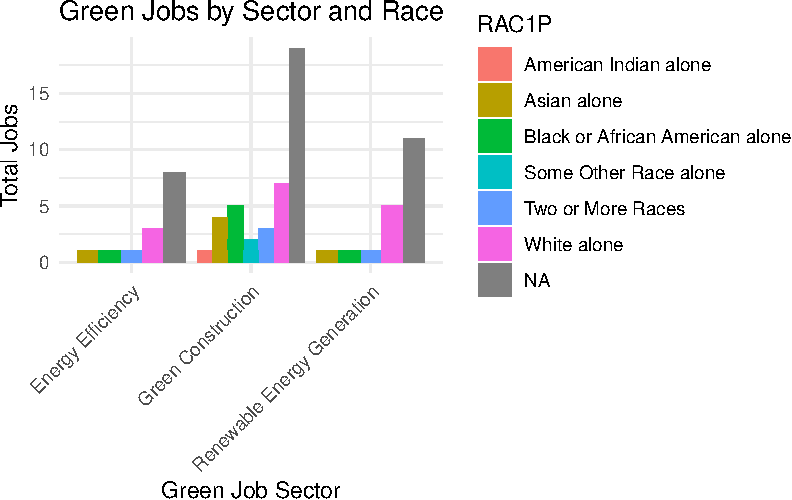
\includegraphics{index_files/figure-pdf/unnamed-chunk-46-1.pdf}

\begin{Shaded}
\begin{Highlighting}[]
\CommentTok{\# Bar plot for green jobs by sector and race (percentage)}
\NormalTok{green\_job\_race\_percentage }\OtherTok{\textless{}{-}}\NormalTok{ merged\_green\_jobs\_data }\SpecialCharTok{\%\textgreater{}\%}
  \FunctionTok{group\_by}\NormalTok{(}\StringTok{\textasciigrave{}}\AttributeTok{O*NET{-}SOC Sector}\StringTok{\textasciigrave{}}\NormalTok{, RAC1P) }\SpecialCharTok{\%\textgreater{}\%}
  \FunctionTok{summarise}\NormalTok{(}\AttributeTok{total\_jobs =} \FunctionTok{n}\NormalTok{()) }\SpecialCharTok{\%\textgreater{}\%}
  \FunctionTok{mutate}\NormalTok{(}\AttributeTok{percentage\_jobs =}\NormalTok{ total\_jobs }\SpecialCharTok{/} \FunctionTok{sum}\NormalTok{(total\_jobs) }\SpecialCharTok{*} \DecValTok{100}\NormalTok{)}
\end{Highlighting}
\end{Shaded}

\begin{verbatim}
`summarise()` has grouped output by 'O*NET-SOC Sector'. You can override using
the `.groups` argument.
\end{verbatim}

\begin{Shaded}
\begin{Highlighting}[]
\FunctionTok{ggplot}\NormalTok{(green\_job\_race\_percentage, }\FunctionTok{aes}\NormalTok{(}\AttributeTok{x =} \StringTok{\textasciigrave{}}\AttributeTok{O*NET{-}SOC Sector}\StringTok{\textasciigrave{}}\NormalTok{, }\AttributeTok{y =}\NormalTok{ percentage\_jobs, }\AttributeTok{fill =}\NormalTok{ RAC1P)) }\SpecialCharTok{+}
  \FunctionTok{geom\_bar}\NormalTok{(}\AttributeTok{stat =} \StringTok{"identity"}\NormalTok{, }\AttributeTok{position =} \StringTok{"dodge"}\NormalTok{) }\SpecialCharTok{+}
  \FunctionTok{labs}\NormalTok{(}\AttributeTok{title =} \StringTok{"Percentage of Green Jobs by Sector and Race"}\NormalTok{,}
       \AttributeTok{x =} \StringTok{"Green Job Sector"}\NormalTok{, }\AttributeTok{y =} \StringTok{"Percentage of Total Jobs"}\NormalTok{) }\SpecialCharTok{+}
  \FunctionTok{theme\_minimal}\NormalTok{() }\SpecialCharTok{+}
  \FunctionTok{theme}\NormalTok{(}\AttributeTok{axis.text.x =} \FunctionTok{element\_text}\NormalTok{(}\AttributeTok{angle =} \DecValTok{45}\NormalTok{, }\AttributeTok{hjust =} \DecValTok{1}\NormalTok{))}
\end{Highlighting}
\end{Shaded}

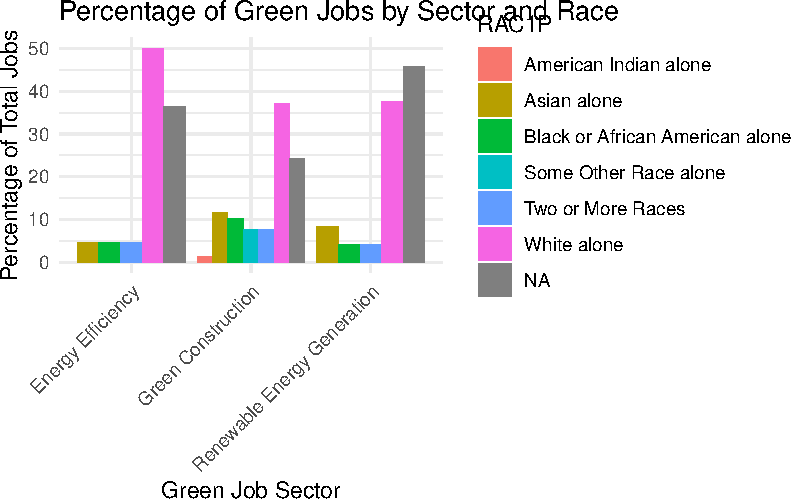
\includegraphics{index_files/figure-pdf/unnamed-chunk-46-2.pdf}

\textsubscript{Source:
\href{https://beeckcenter.github.io/climate-equity-workforce/index-preview.html}{Article
Notebook}}

\begin{Shaded}
\begin{Highlighting}[]
\CommentTok{\# Bar plot for green jobs by sector and gender}
\FunctionTok{ggplot}\NormalTok{(green\_job\_summary, }\FunctionTok{aes}\NormalTok{(}\AttributeTok{x =} \StringTok{\textasciigrave{}}\AttributeTok{O*NET{-}SOC Sector}\StringTok{\textasciigrave{}}\NormalTok{, }\AttributeTok{y =}\NormalTok{ total\_jobs, }\AttributeTok{fill =}\NormalTok{ SEX)) }\SpecialCharTok{+}
  \FunctionTok{geom\_bar}\NormalTok{(}\AttributeTok{stat =} \StringTok{"identity"}\NormalTok{, }\AttributeTok{position =} \StringTok{"dodge"}\NormalTok{) }\SpecialCharTok{+}
  \FunctionTok{labs}\NormalTok{(}\AttributeTok{title =} \StringTok{"Green Jobs by Sector and Gender"}\NormalTok{,}
       \AttributeTok{x =} \StringTok{"Green Job Sector"}\NormalTok{, }\AttributeTok{y =} \StringTok{"Total Jobs"}\NormalTok{) }\SpecialCharTok{+}
  \FunctionTok{theme\_minimal}\NormalTok{() }\SpecialCharTok{+}
  \FunctionTok{theme}\NormalTok{(}\AttributeTok{axis.text.x =} \FunctionTok{element\_text}\NormalTok{(}\AttributeTok{angle =} \DecValTok{45}\NormalTok{, }\AttributeTok{hjust =} \DecValTok{1}\NormalTok{))}
\end{Highlighting}
\end{Shaded}

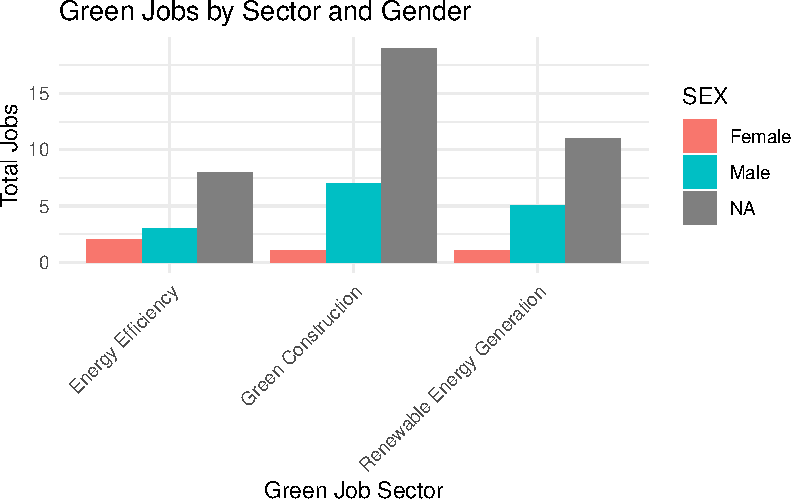
\includegraphics{index_files/figure-pdf/unnamed-chunk-47-1.pdf}

\begin{Shaded}
\begin{Highlighting}[]
\CommentTok{\# Bar plot for green jobs by sector and gender (percentage)}
\NormalTok{green\_job\_gender\_percentage }\OtherTok{\textless{}{-}}\NormalTok{ merged\_green\_jobs\_data }\SpecialCharTok{\%\textgreater{}\%}
  \FunctionTok{group\_by}\NormalTok{(}\StringTok{\textasciigrave{}}\AttributeTok{O*NET{-}SOC Sector}\StringTok{\textasciigrave{}}\NormalTok{, SEX) }\SpecialCharTok{\%\textgreater{}\%}
  \FunctionTok{summarise}\NormalTok{(}\AttributeTok{total\_jobs =} \FunctionTok{n}\NormalTok{()) }\SpecialCharTok{\%\textgreater{}\%}
  \FunctionTok{mutate}\NormalTok{(}\AttributeTok{percentage\_jobs =}\NormalTok{ total\_jobs }\SpecialCharTok{/} \FunctionTok{sum}\NormalTok{(total\_jobs) }\SpecialCharTok{*} \DecValTok{100}\NormalTok{)}
\end{Highlighting}
\end{Shaded}

\begin{verbatim}
`summarise()` has grouped output by 'O*NET-SOC Sector'. You can override using
the `.groups` argument.
\end{verbatim}

\begin{Shaded}
\begin{Highlighting}[]
\FunctionTok{ggplot}\NormalTok{(green\_job\_gender\_percentage, }\FunctionTok{aes}\NormalTok{(}\AttributeTok{x =} \StringTok{\textasciigrave{}}\AttributeTok{O*NET{-}SOC Sector}\StringTok{\textasciigrave{}}\NormalTok{, }\AttributeTok{y =}\NormalTok{ percentage\_jobs, }\AttributeTok{fill =}\NormalTok{ SEX)) }\SpecialCharTok{+}
  \FunctionTok{geom\_bar}\NormalTok{(}\AttributeTok{stat =} \StringTok{"identity"}\NormalTok{, }\AttributeTok{position =} \StringTok{"dodge"}\NormalTok{) }\SpecialCharTok{+}
  \FunctionTok{labs}\NormalTok{(}\AttributeTok{title =} \StringTok{"Percentage of Green Jobs by Sector and Gender"}\NormalTok{,}
       \AttributeTok{x =} \StringTok{"Green Job Sector"}\NormalTok{, }\AttributeTok{y =} \StringTok{"Percentage of Total Jobs"}\NormalTok{) }\SpecialCharTok{+}
  \FunctionTok{theme\_minimal}\NormalTok{() }\SpecialCharTok{+}
  \FunctionTok{theme}\NormalTok{(}\AttributeTok{axis.text.x =} \FunctionTok{element\_text}\NormalTok{(}\AttributeTok{angle =} \DecValTok{45}\NormalTok{, }\AttributeTok{hjust =} \DecValTok{1}\NormalTok{))}
\end{Highlighting}
\end{Shaded}

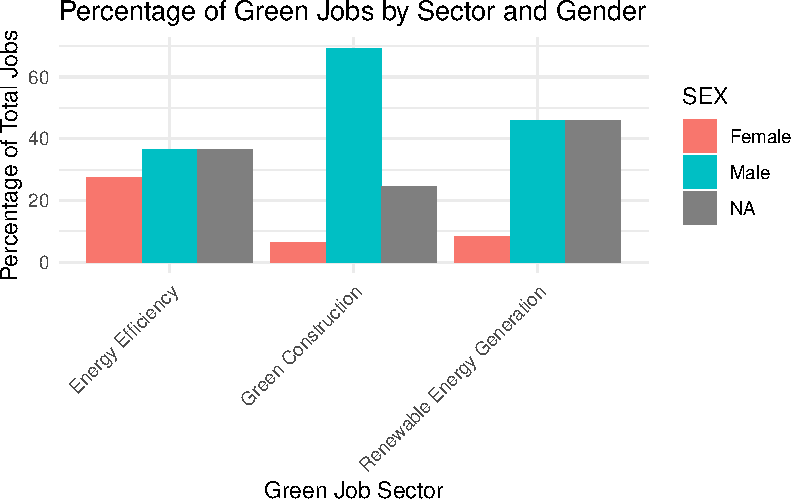
\includegraphics{index_files/figure-pdf/unnamed-chunk-47-2.pdf}

\textsubscript{Source:
\href{https://beeckcenter.github.io/climate-equity-workforce/index-preview.html}{Article
Notebook}}

\begin{Shaded}
\begin{Highlighting}[]
\CommentTok{\# Box plot for income distribution by sector and education level}
\FunctionTok{ggplot}\NormalTok{(merged\_green\_jobs\_data, }\FunctionTok{aes}\NormalTok{(}\AttributeTok{x =} \StringTok{\textasciigrave{}}\AttributeTok{O*NET{-}SOC Sector}\StringTok{\textasciigrave{}}\NormalTok{, }\AttributeTok{y =}\NormalTok{ PINCP, }\AttributeTok{fill =}\NormalTok{ RAC1P)) }\SpecialCharTok{+}
  \FunctionTok{geom\_boxplot}\NormalTok{() }\SpecialCharTok{+}
  \FunctionTok{labs}\NormalTok{(}\AttributeTok{title =} \StringTok{"Income Distribution by Sector and Education Level"}\NormalTok{,}
       \AttributeTok{x =} \StringTok{"Green Job Sector"}\NormalTok{, }\AttributeTok{y =} \StringTok{"Personal Income"}\NormalTok{) }\SpecialCharTok{+}
  \FunctionTok{theme\_minimal}\NormalTok{() }\SpecialCharTok{+}
  \FunctionTok{theme}\NormalTok{(}\AttributeTok{axis.text.x =} \FunctionTok{element\_text}\NormalTok{(}\AttributeTok{angle =} \DecValTok{45}\NormalTok{, }\AttributeTok{hjust =} \DecValTok{1}\NormalTok{))}
\end{Highlighting}
\end{Shaded}

\begin{verbatim}
Warning: Removed 38 rows containing non-finite outside the scale range
(`stat_boxplot()`).
\end{verbatim}

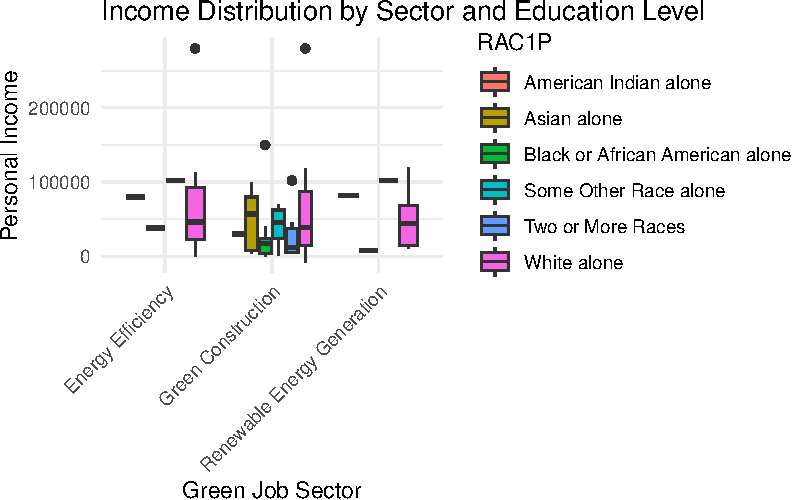
\includegraphics{index_files/figure-pdf/unnamed-chunk-48-1.pdf}

\textsubscript{Source:
\href{https://beeckcenter.github.io/climate-equity-workforce/index-preview.html}{Article
Notebook}}



\end{document}
